% XeLaTeX can use any Mac OS X font. See the setromanfont command below.
% Input to XeLaTeX is full Unicode, so Unicode characters can be typed directly into the source.

% The next lines tell TeXShop to typeset with xelatex, and to open and save the source with Unicode encoding.

%!TEX TS-program = xelatex
%!TEX encoding = UTF-8 Unicode

\documentclass[11pt,twoside]{book}
\usepackage{multirow}
\usepackage{pdfpages}

\usepackage{geometry}                % See geometry.pdf to learn the layout options. There are lots.
%\usepackage[margin=1cm]{geometry}


%	\addtolength{\textwidth}{1.75in}
%
%	\addtolength{\topmargin}{-.875in}
%	\addtolength{\textheight}{1.75in}

\geometry{a4paper,left=20mm,top=20mm,total={162mm,230mm}}                   % ... or a4paper or a5paper or ... 
%\geometry{landscape}                % Activate for for rotated page geometry
%\usepackage[parfill]{parskip}    % Activate to begin paragraphs with an empty line rather than an indent

\setcounter{secnumdepth}{5}

\usepackage{amssymb}
%\usepackage{todonotes}
\setlength{\marginparwidth}{2cm}
\usepackage[backgroundcolor=white,bordercolor=blue,linecolor=blue,textwidth=1cm]{todonotes}
\usepackage{booktabs}
\usepackage{longtable}
\usepackage{url}

\usepackage[depth=4]{bookmark}


\usepackage{algorithm}
\usepackage{algpseudocode}

\usepackage{imakeidx}
\usepackage[utf8]{inputenc}
\usepackage[T1]{fontenc}
\makeindex[intoc]

\usepackage[font=normalsize]{caption}  

\usepackage{hyperref}
\hypersetup{
    colorlinks,
    citecolor=black,
    filecolor=black,
    linkcolor=black,
    urlcolor=black
}

\usepackage{xcolor}
\usepackage{listings}

\makeatletter
\global\let\tikz@ensure@dollar@catcode=\relax
\makeatother

\definecolor{mGreen}{rgb}{0,0.6,0}
\definecolor{mGray}{rgb}{0.5,0.5,0.5}
\definecolor{mPurple}{rgb}{0.58,0,0.82}
\definecolor{backgroundColour}{rgb}{0.95,0.95,0.92}
\definecolor{gray}{rgb}{0.4,0.4,0.4}
\definecolor{darkblue}{rgb}{0.0,0.0,0.6}
\definecolor{cyan}{rgb}{0.0,0.6,0.6}

\lstdefinestyle{CStyle}{
    backgroundcolor=\color{backgroundColour},   
    commentstyle=\color{mGreen},
    keywordstyle=\color{magenta},
    numberstyle=\tiny\color{mGray},
    stringstyle=\color{mPurple},
    basicstyle=\scriptsize\ttfamily,
    breakatwhitespace=false,         
    breaklines=true,                 
    captionpos=b,                    
    keepspaces=true,                 
    numbers=left,                    
    numbersep=5pt,                  
    showspaces=false,                
    showstringspaces=false,
    showtabs=false,                  
    tabsize=2,
    language=C
}


\lstset{ 
  backgroundcolor=\color{white},   % choose the background color; you must add \usepackage{color} or \usepackage{xcolor}; should come as last argument
  basicstyle=\footnotesize\ttfamily,        % the size of the fonts that are used for the code
  breakatwhitespace=false,         % sets if automatic breaks should only happen at whitespace
  breaklines=true,                 % sets automatic line breaking
  captionpos=b,                    % sets the caption-position to bottom
  commentstyle=\color{gray},    % comment style
  deletekeywords={...},            % if you want to delete keywords from the given language
  %escapeinside={\%*}{*)},          % if you want to add LaTeX within your code
  %extendedchars=true,              % lets you use non-ASCII characters; for 8-bits encodings only, does not work with UTF-8
  %firstnumber=1000,                % start line enumeration with line 1000
  frame=single,	                   % adds a frame around the code
  keepspaces=true,                 % keeps spaces in text, useful for keeping indentation of code (possibly needs columns=flexible)
  keywordstyle=\color{blue},       % keyword style
  language=C,                 % the language of the code
  %morekeywords={*,...},            % if you want to add more keywords to the set
  numbers=left,                    % where to put the line-numbers; possible values are (none, left, right)
  numbersep=5pt,                   % how far the line-numbers are from the code
  numberstyle=\tiny\color{gray}, % the style that is used for the line-numbers
  rulecolor=\color{black},         % if not set, the frame-color may be changed on line-breaks within not-black text (e.g. comments (green here))
  showspaces=false,                % show spaces everywhere adding particular underscores; it overrides 'showstringspaces'
  showstringspaces=false,          % underline spaces within strings only
  showtabs=false,                  % show tabs within strings adding particular underscores
  stepnumber=1,                    % the step between two line-numbers. If it's 1, each line will be numbered
  stringstyle=\color{black},     % string literal style
  tabsize=2,	                   % sets default tabsize to 2 spaces
}

\lstset{
  columns=fullflexible,
  showstringspaces=false,
  commentstyle=\color{gray}\upshape,
  backgroundcolor=\color{backgroundColour},   
  commentstyle=\color{mGreen},
  keywordstyle=\color{magenta},
  numberstyle=\tiny\color{mGray},
  stringstyle=\color{mPurple},
  basicstyle=\scriptsize\ttfamily,
  tabsize=2
}

\lstdefinelanguage{XML}
{
  morestring=[b]",
  morestring=[s]{>}{<},
  morecomment=[s]{<?}{?>},
  stringstyle=\color{black},
  identifierstyle=\color{darkblue},
  keywordstyle=\color{cyan},
  morekeywords={xmlns,version,type}% list your attributes here
}


% Will Robertson's fontspec.sty can be used to simplify font choices.
% To experiment, open /Applications/Font Book to examine the fonts provided on Mac OS X,
% and change "Hoefler Text" to any of these choices.

\renewcommand{\scriptsize}{\tiny}

\usepackage{fontspec,xltxtra,xunicode}
\defaultfontfeatures{Mapping=tex-text}
\setromanfont[Scale=MatchLowercase,Mapping=tex-text]{Optima}
\setsansfont[Scale=MatchLowercase,Mapping=tex-text]{Optima}
\setmonofont[Scale=MatchLowercase]{Andale Mono}

%%%% Graphics
\usepackage{graphicx}
\usepackage{tikz}
\definecolor{unilublue}{RGB}{55,149,218}
\definecolor{sntred}{RGB}{219,46,27}
\definecolor{sntpurple}{RGB}{86,30,130}
%\definecolor{sntblue}{RGB}{50,130,207}
\definecolor{sntblue}{RGB}{55,149,218}

\pgfdeclareimage[width=30mm]{logo-snt}{logos/logo-snt}
\pgfdeclareimage[width=30mm]{logo-uni-lu}{logos/logo-uni-lu}

%%%% Fancy
\usepackage{fancyhdr}

%%%% Increase page length
\addtolength{\textheight}{1in}

%%%% Sections
\usepackage{xspace}
\usepackage{sectsty}
\allsectionsfont{\sffamily}

\setlength{\parskip}{1em}

%\renewcommand{\,}{$^{\cdot}$}

%%%% Title
\newcommand{\titleone}{\textsf{D4}}
\newcommand{\titletwo}{\textsf{Validation of the toolset}}
\newcommand{\titlethree}{\textsf{}}

\newcommand{\todoinline}[1]{\todo[color=orange,inline]{ \textbf{TODO}: #1 }}

\newcommand{\TODO}[1]{\todo[color=orange,inline]{ \textbf{TODO}: #1 }}
\newcommand{\DONE}[1]{\todo[color=green,inline]{ \textbf{DONE}: #1 }}


\usepackage{amsmath}
\usepackage{array}
\usepackage{lipsum}

\usepackage{algorithm}
\usepackage{algpseudocode}

\newcommand{\LXS}{LXS\xspace{}}
\newcommand{\GSL}{GSL\xspace{}}
\newcommand{\ESA}{ESA\xspace{}}
\newcommand{\ESAIL}{ESAIL\xspace}
\newcommand{\PARAM}{LIBPARAM\xspace}
\newcommand{\UTIL}{LIBUTIL\xspace}

\newcommand{\GomSpace}{GomSpace\xspace}
\newcommand{\LuxSpace}{LuxSpace\xspace}
\newcommand{\ONE}{GSL\xspace}
\newcommand{\TWO}{LXS\xspace}
\newcommand{\CITONE}{~\cite{GSL}}
\newcommand{\CITTWO}{~\cite{LXS}}
\newcommand{\LAUNCH}{on September 2020~\cite{ESAILlaunch}}
\newcommand{\OPENCSP}{the open source CubeSat Space Protocol (\CSP) library~\cite{CSP}}


\newcommand{\ADCS}{\emph{\ESAIL-ADCS}\xspace}
\newcommand{\GPS}{\emph{\ESAIL-GPS}\xspace}
\newcommand{\PDHU}{\emph{\ESAIL-PDHU}\xspace}
\newcommand{\SVF}{\emph{\ESAIL-SVF}\xspace}

\newcommand{\FIXME}[1]{#1}

\newcommand{\CHANGED}[1]{\textcolor{black}{#1}}
\newcommand{\CHANGEDTWO}[1]{\textcolor{black}{#1}}
\newcommand{\CHANGEDOCT}[1]{\textcolor{black}{#1}}
\newcommand{\CHANGEDNOV}[1]{\textcolor{black}{#1}}

\newcommand{\TRFOUR}[1]{\textcolor{green}{#1}}

\newcommand{\STARTCHANGEDNOV}{\color{black}}
\newcommand{\ENDCHANGEDNOV}{\color{black}}

\newcommand{\STARTCHANGEDWPT}{\color{black}}
\newcommand{\ENDCHANGEDWPT}{\color{black}}


%\newcommand{\MREVISION}[2]{\todo{\tiny{#1}}\textcolor{blue}{#2}}
\newcommand{\MREVISION}[2]{#2}

%\newcommand{\REVTWO}[2]{\todo[color=red]{\tiny{#1}}\textcolor{red}{#2}}
\newcommand{\REVTWO}[2]{#2}

\newcommand{\REVNOV}[2]{\textcolor{black}{#2}}

\newcommand{\REVOCT}[2]{\todo{\tiny{#1}}\textcolor{blue}{#2}}
\newcommand{\REVTOOL}[2]{\todo{\tiny{#1}}\textcolor{blue}{#2}}

\newcommand{\EMPH}[1]{\textbf{\emph{#1}}}
\newcommand{\INDEX}[1]{\index{\MakeLowercase{#1}}\EMPH{#1}}

\newcommand{\APPR}{\emph{SMTS}\xspace}

\begin{document}

\pagestyle{fancy}
\renewcommand{\sectionmark}[1]{\markright{\textit{#1}}}

\renewcommand{\headrulewidth}{2pt}% 2pt header rule
\renewcommand{\headrule}{\hbox to\headwidth{%
  \color{sntblue}\leaders\hrule height \headrulewidth\hfill}}

\fancyhf{}

%\lhead{\fancyplain{}{\setlength{\unitlength}{1mm}
%\begin{picture}(0,0)
%\put(0,-4){
\includegraphics[width=50pt]{logos/logo-snt}}
%\end{picture}}} 

\lhead{\fancyplain{}{\textit{}}}

\rhead{\fancyplain{}{\rightmark }}

\fancyfoot[C]{%
\begin{tikzpicture}[remember picture,overlay]
\path [fill=sntred]    ([xshift=88pt,yshift=20pt]current page.south west) rectangle
                       ([xshift=229pt,yshift=30pt] current page.south west);
\path [fill=sntpurple] ([xshift=229pt,yshift=20pt] current page.south west) rectangle
                       ([xshift=370pt,yshift=30pt] current page.south west);
\path [fill=sntblue]   ([xshift=370pt,yshift=20pt] current page.south west) rectangle
                       ([xshift=510pt,yshift=30pt] current page.south west);
\end{tikzpicture}
}

\fancyfoot[RO]{
\begin{tikzpicture}[remember picture,overlay]
\node [circle, ultra thick, fill=white, draw=sntblue] at ([xshift=530pt,yshift=35pt] current page.south west) {\thepage};
\end{tikzpicture}}

\fancyfoot[LE]{
\begin{tikzpicture}[remember picture,overlay]
\node [circle, ultra thick, fill=white, draw=sntblue] at ([xshift=65pt,yshift=35pt] current page.south west) {\thepage};
\end{tikzpicture}}

\newcommand{\JMR}[2]{\textcolor{black}{#2}}
\newcommand{\NEWFSCI}[1]{\textcolor{black}{#1}}

\newcommand{\JMRCHANGE}[1]{\textcolor{black}{#1}}
\newcommand{\UPDATE}[1]{\textcolor{black}{#1}}

\newcommand{\SAIL}{\emph{ESAIL}\xspace}
\newcommand{\MLFS}{\emph{MLFS}\xspace}
\newcommand{\GCSP}{\emph{LIBGCSP}\xspace}

\newcommand{\MPTS}{\emph{MASS-reduced} test suite\xspace}
\newcommand{\MPTSs}{\emph{MASS-reduced} test suites\xspace}
\newcommand{\ExaE}{ExactEarth}

\newcommand{\prog}{P}
\newcommand{\prop}{}




\thispagestyle{empty}

\begin{tikzpicture}[remember picture,overlay]
\path [fill=sntred]    ([xshift=30pt,yshift=20pt]current page.south west) rectangle
                       ([xshift=210pt,yshift=50pt] current page.south west);
\path [fill=sntpurple] ([xshift=210pt,yshift=20pt] current page.south west) rectangle
                       ([xshift=390pt,yshift=50pt] current page.south west);
\path [fill=sntblue]   ([xshift=390pt,yshift=20pt] current page.south west) rectangle
                       ([xshift=570pt,yshift=51pt] current page.south west);
\path [fill=unilublue] ([xshift=30pt,yshift= 50pt] current page.south west) --
                       ([xshift=570pt,yshift= 50pt] current page.south west)
                       [rounded corners=20pt] --
                       ([xshift=570pt,yshift=740pt] current page.south west)
                       [sharp corners] --
                       ([xshift=30pt,yshift=740pt] current page.south west);
\node [fill=white,rounded corners=0pt,inner xsep=6pt,inner ysep=3pt]
      at ([xshift=523pt,yshift=120pt] current page.south west)
      {\pgfuseimage{logo-uni-lu}};

\node [fill=white,rounded corners=2pt,inner xsep=6pt,inner ysep=3pt]
      at ([xshift=520pt,yshift=780pt] current page.south west)
      {\pgfuseimage{logo-snt}};

%\node [circle, fill=white, draw=sntblue] at ([xshift=550pt,yshift=35pt] current page.south west) {a};

\node[draw=none,fill=none,right] at (-1, -7){\color{white}\LARGE\bf\titleone};
\node[draw=none,fill=none,right] at (-1, -8){\color{white}\LARGE\bf\titletwo};
\node[draw=none,fill=none,right] at (-1, -9){\color{white}\LARGE\bf\titlethree};

\node[draw=none,fill=none,right] at (-1, -12){\color{white}\Large\textsf{O. Cornejo, F. Pastore, E. Viganò}};
\node[draw=none,fill=none,right] at (-1, -13){\color{white}\Large\textsf{Interdisciplinary Centre for Security, Reliability and Trust}};
\node[draw=none,fill=none,right] at (-1, -14){\color{white}\Large\textsf{University of Luxembourg}};
\node[draw=none,fill=none,right] at (11, -16){\color{white}\textsf{ITT-1-9873-ESA-FAQAS-SUTP}};
\node[draw=none,fill=none,right] at (11, -17){\color{white}\Large\textsf{Issue 4, Rev. 1}};
\node[draw=none,fill=none,right] at (11, -18){\color{white}\Large\textsf{\today}};
\node[draw=none,fill=none,right] at (-1, -24){\color{white}\tiny\textsf{EUROPEAN SPACE AGENCY. CONTRACT REPORT.}};
\node[draw=none,fill=none,right] at (-1, -24.3){\color{white}\tiny\textsf{The work described in this report was done under ESA contract. Responsibility for the contents resides in the author or organisation that prepared it.}};
\node[draw=none,fill=none,right] at (-1, -24.8){\color{white}\tiny\textsf{The copyright in this document is vested in the University of Luxembourg.}};
\node[draw=none,fill=none,right] at (-1, -25.1){\color{white}\tiny\textsf{This document may only be reproduced in whole or in part, or stored in a retrieval system,or transmitted in any form, or by any means electronic,}};
\node[draw=none,fill=none,right] at (-1, -25.4){\color{white}\tiny\textsf{mechanical, photocopying or otherwise, either with the prior permission of the University of Luxembourg or in accordance with the terms of ESTEC Contract No. 4000128969/19/NL/AS.}};

\node[draw=none,fill=none,right] at (-1, -24){\color{white}\tiny\textsf{EUROPEAN SPACE AGENCY. CONTRACT REPORT.}}; 
\node[draw=none,fill=none,right] at (-1, -24.3){\color{white}\tiny\textsf{The work described in this report was done under ESA contract. Responsibility for the contents resides in the author or organisation that prepared it.}};
\node[draw=none,fill=none,right] at (-1, -24.8){\color{white}\tiny\textsf{The copyright in this document is vested in the University of Luxembourg.}};
\node[draw=none,fill=none,right] at (-1, -25.1){\color{white}\tiny\textsf{This document may only be reproduced in whole or in part, or stored in a retrieval system,or transmitted in any form, or by any means electronic,}}; 
\node[draw=none,fill=none,right] at (-1, -25.4){\color{white}\tiny\textsf{mechanical, photocopying or otherwise, either with the prior permission of the University of Luxembourg or in accordance with the terms of ESTEC Contract No. 4000128969/19/NL/AS.}};


\end{tikzpicture}

\newpage


% !TEX root = MAIN.tex

\section*{Revisions}
\label{sec:revisions}


\setlength\LTleft{0pt}
\setlength\LTright{0pt}
\tiny 
%@{\extracolsep{\fill}}
\begin{longtable}{|p{2cm}|p{1cm}|p{1.5cm}|p{9cm}|@{}}
\label{table:codeoperators} \\
\hline
\textbf{Issue Number}&\textbf{Date}&\textbf{Authors}&\textbf{Description}\\
\hline
ITT-1-9873-ESA-FAQAS-FR
Issue 1 Rev. 1&
October 29th, 2021&
Fabrizio Pastore, Oscar Cornejo, Enrico Viganò&
\begin{minipage}{8cm}
Initial release.
\end{minipage}
\\
\hline
ITT-1-9873-ESA-FAQAS-FR
Issue 1 Rev. 2&
November 11th, 2021&
Fabrizio Pastore, Oscar Cornejo, Enrico Viganò&
\begin{minipage}{8cm}
Added Chapter~\ref{chap:deliverables_summary} (deliverables summary).\\
Added Chapter~\ref{ch:toolset} (description of toolset package).\\
Added information about input and outputs of the tools in Chapter~\ref{chapter:methodology} (see blue text).
\end{minipage}
\\
\hline
                                                    
\end{longtable}
\normalsize

\clearpage

% !TEX root = MAIN.tex

\section*{Delivered Items}
\label{sec:deliverables}

In the following Table we provide a list of deliverable items released with this document. Each Item is identified by it's path on the Alfresco system.

\setlength\LTleft{0pt}
\setlength\LTright{0pt}
\tiny 
%@{\extracolsep{\fill}}
\begin{longtable}{|p{9cm}|p{6cm}@{}}
\label{table:deliverables} \\
\hline
\textbf{Deliverable}&Description\\
\hline
ASN1CC-CaseStudy/Specifications/ACN-UM-v-3-2.pdf&User manual of ASN1 Compiler\\
ASN1CC-CaseStudy/Specifications/taste-documentation-current.pdf&Taste software documentation including ASN1 overview\\
\hline
GSL-CaseStudies/Specifications/gs-man-nanosoft-ms100-command-and-management-sdk-3.6.2-1-g67fe6e1.pdf&LXS softwrae specifications\\
\hline
LXS-CaseStudies/Specifications&Folder with LXS specifications\\
LXS-CaseStudies/Specifications/FAQAS-LXS-MAN-001\_1- SVF Software Installation and User Manual.pdf&SVF and ESAIL Software Installation and User Manual\\
LXS-CaseStudies/Specifications/ESAIL-LXS-ICD-P-0184\_2A ADCS IF SW External ICD.docx&\\
LXS-CaseStudies/Specifications/ESAIL-LXS-SDD-P-0105\_1B On-board Application Software Design Document&\\
LXS-CaseStudies/Specifications/MOC-applicable MIB egos-mcs-s2k-icd-0001-version7.0-FINAL&SCOS-2000 Database Import ICD\\
LXS-CaseStudies/Specifications/ocp.dat&SCOS-2000 Database file containing the specifications of the nominal value ranges for ESAIL ADCS parameters.\\
\hline
SnT-Software/FAQAS-DataDrivenMutator-Buffers.zip&Preliminary implementation of the data-driven mutation testing component\\
%\begin{minipage}{8cm}
%Initial release.
%\end{minipage}
\\
\hline

%ITT-1-9873-ESA-FAQAS-D1
%Issue 4
%&DATE
%&Fabrizio Pastore, Oscar Cornejo
%&
%\begin{minipage}{8cm}
%\end{minipage}
%\\

%\hline
                                                    
\end{longtable}
\normalsize

\clearpage



\tableofcontents



% !TEX root = MAIN.tex

\chapter{Scope and content}

This document is the deliverable SSS of the ESA activity ITT-1-9873-ESA. It concerns requirements specification for the \emph{FAQAS framework} to be delivered by ITT-1-9873-ESA. Following the structure described in the SoW \emph{AO9873-ws00pe\_SOW.pdf}, it provides the structured requirements baseline for the FAQAS framework according to ECSS-E-ST-40C Annex B.
 
\section{Applicable and reference documents}

\begin{itemize}
\item{D1 - Mutation testing survey}
\item{D2 - Study of mutation testing applicability to space software}
\end{itemize}

\chapter{Terms, definitions and abbreviated terms}

\begin{itemize}
\item{FAQAS}: activity ITT-1-9873-ESA
\item{FAQAS-framework}: software system to be released at the end of WP4 of FAQAS
\item{D2}: Deliverable D2 of FAQAS, \emph{Study of mutation testing applicability to space software}
\item{KLEE}: Third party test generation tool, details are provided in D2.
\item{SUT}: Software under test, i.e, the software that should be mutated by means of mutation testing.
\item{WP}: Work package
\end{itemize}

\clearpage
 



% !TEX root = MAIN.tex

\section{Acronyms and Abbreviations}
\label{sec:acronyms}


%@{\extracolsep{\fill}}
\begin{tabular}{|p{1.5cm}|p{14.5cm}|}
%&\TODO{Add acronyms. OSCAR: I've add some...} \\

%ACO & Ant Colony Optimization\\
D1& Deliverable 1 of FAQAS activity, \emph{Analysis and Survey of Mutation Testing}\\
D2& Deliverable 2 of FAQAS activity, \emph{Study of Mutation Testing Applicability to Space Software}\\
FOM & First Order Mutant\\
HOM & Higher-Order Mutant\\
LOC & Lines of Code\\
%SBST & Search Based Software Testing\\
%Fabrizio: we cannot use SE as acronym
%SE & Symbolic Execution\\
SOM & Second Order Mutant\\
SUT & Software Under Test\\
TS & Test Suite\\
UL HPC & University of Luxembourg High Performance Computing

%Comment #2:
%When generating the pdf file, make sure to have the index of the document on the left, so that the document is easier to navigate.
%Author: Pedro Barrios Subject: Sticky Note Date: 28/02/2020, 09:18:06
%Comment #3:
%Try to make the document a bit more friendly to read (e.g. by adding some sentences in bold (see the highlighted ones for this paragraph), making bigger
%separation between paragraphs, ...)
%Author: Pedro Barrios Subject: Sticky Note Date: 28/02/2020, 09:18:11
%Comment #4:
%It is perhaps interesting to add a chapter with some basic definitions?
%e.g. equivalent mutant, redundant mutant, mutation score, killed mutant, live mutant, weak mutation, ...
%Author: Pedro Barrios Subject: Sticky Note Date: 28/02/2020, 09:18:18
%Comment #5:
%Please, consider to add more examples.

                                                           
\end{tabular}
\normalsize

\clearpage

\include{casestudies}

\chapter{FAQAS validation results}
\label{ch:results}

% !TEX root = MAIN.tex
\clearpage
\section{Code-driven Mutation Analysis}
\label{sec:testSuiteEvaluation:codeDriven}



% !TEX root =  Main.tex



\subsection{Overview}
\label{sec:evaluation}

\renewcommand{\APPR}{\textit{MASS}\xspace}

\STARTCHANGEDNOV

Our empirical evaluation aims to assess the effectiveness of the techniques integrated into \INDEX{\APPR} to address scalability and pertinence problems (i.e., Steps 2, 4, 5, 6, 7, and 8 of \APPR). Our objectives include (RQ1) confirming, in our context, trivial compiler optimization results observed in related work (Step 4), (RQ2) identifying the most effective solution for mutants sampling (Step 5), (RQ3) comparing mutants generation strategies implemented by \APPR (Step 2), evaluating the (RQ4) accuracy and (RQ5) effectiveness of the strategies proposed  for test suite prioritization (Step 6), and (RQ6) evaluating the accuracy of the strategy for the identification of likely equivalent/duplicate mutants (Step 7). Finally, we aim to (RQ7) compare the mutation score computed by \APPR (Step 8) with the mutation score computed without \APPR optimizations.
\REVNOV{C-P-11}{The project will include continuous empirical evaluation sessions with the case study systems that aim to address the following research questions:}

%Our empirical evaluation aims to address the following research questions, in the context of embedded space software:

\begin{itemize}

    \item[RQ1] \JMRCHANGE{(Step 4)} What are the cost savings provided by compiler optimization techniques detecting equivalent and duplicate mutants?
    We wish to determine what is the percentage of mutants reported as being equivalent and duplicate by compiler optimization techniques. After accounting for the additional compilation time entailed by such techniques, we want to identify the optimal subset of compilation options to be used in Step 4 of \APPR.

    \item[RQ2] \JMRCHANGE{(Step 5)} Can a randomly selected subset of mutants be used to accurately estimate the mutation score obtained from the entire set of mutants? 
    \CHANGED{We attempt to evaluate four mutants sampling strategies: \INDEX{proportional uniform sampling}, \INDEX{proportional method-based sampling},  \INDEX{uniform fixed-size sampling}, and \INDEX{uniform FSCI sampling}. More precisely, we aim to determine the best configuration for each sampling strategy (i.e., sampling ratio, sample size, and confidence interval). Furthermore, we need to identify which strategy offers the best trade-off between the number of mutants to be tested and accuracy.}
%    We attempt to replicate the findings reported by Zhang et al.~\cite{zhang2013operator} and determine the optimal sampling ratio to be used in \APPR Step 5.

    %Additionally we may ask, do these results generalize for mutants that are generated with mutation operators that are others than the sufficient set?

   % \item[RQ3] Can we identify the minimal number of randomly selected mutants enabling the accurate estimation of the mutation score for the entire set of mutants? RQ3 aims to replicate the findings reported in~\cite{gopinath2015hard}. 

    \item[RQ3]  {Do mutants generated with deletion operators (i.e., SDL and OODL) lead to a mutation score that accurately estimates the mutation score of the entire set of mutants?  
    \REVNOV{PTCR-P-13}{Recall from Section 1.2.1.2 from D2 that SDL and \INDEX{OODL operators} present the following advantages (1) the set of SDL and OODL operators is smaller than the sufficient set thus they lead to less mutants, (2) they are simpler to implement, (3) they produce significantly less equivalent mutants, and (4) test suites that kill mutants generated with both the SDL and the \INDEX{OODL operators} kill a very high percentage of all mutants~\cite{delamaro2014experimental}.}
   We want to determine if we can minimize the number of selected mutants by only relying on deletion operators. To do so, we compare the mutation score generated with SDL and OODL operators with the mutation score based on all available mutation operators. }
    %The results from RQ2, RQ3, and RQ4 will help us determine the best sampling strategy to adopt in \APPR Step 5.
    
    
    \item[RQ4] \JMRCHANGE{(Step 6)} Can a prioritized subset of test cases that maximizes test suite diversity be used to accurately estimate the mutation score of the entire test suite?
    We investigate how the various distance metrics used in the PrioritizeAndReduce algorithm implemented by \APPR  (Step 6) compare in terms of accuracy. 
    
    %Results from RQ2 and RQ3 will guide the selection of the distance metric to be used with \APPR.

    \item[RQ5] \JMRCHANGE{(Step 6)} To what extent different test suite prioritization strategies can speed up the mutation analysis process? We investigate the execution time reduction achieved by different distance metrics used in the PrioritizeAndReduce algorithm. 
    

    \item[RQ6] \JMRCHANGE{(Step 7)} Is it possible to identify thresholds, based on code coverage information, that enable the detection of nonequivalent and nonduplicate mutants? We investigate 
    the accuracy of our strategy 
    %for identifying nonequivalent and nonduplicate mutants
    %how accurate are the equivalent and duplicate mutants detected 
    based on threshold values for the best distance metric  (\APPR  Step 7).
    
    % \item[RQ9] Do mutants generated with operators that modify the control-flow produce less equivalent mutants? This research questions aims to replicate the findings reported in~\cite{schuler2013covering}.

    \item[RQ7] \JMRCHANGE{(Step 8)} How does the mutation score computed by \APPR relate to the mutation score of the original test suite based on the complete set of mutants? In other words, is there any tradeoff between the gains in scalability due to \APPR and  mutation score accuracy? We therefore analyze the difference between the \APPR mutation score, which is obtained with a subset of the test suite and excludes likely equivalent and duplicate mutants, and the mutation score obtained with the entire set of mutants tested with the full test suite.
    
    \item[RQ8] \REVNOV{C-P-5}{Is it possible to identify a threshold for the mutation score that ensures that the fault revealing power of a test suite is greater than the one of a test suite that simply achieves statement coverage adequacy (i.e., all the statements are covered)?}
    
    \item[RQ9] Can mutation analysis results be computed by combining results obtained with different test suites?


    
\end{itemize}

%In principle we should use the same metrics used in those papers or justify why we use different ones.

%For RQ1 - RQ5, Can we execute all the mutants? Should we select a subset of the components? Does this choice introduce a bias?

\subsection{Subjects of the study}
\label{sec:empirical:subjects}

To perform our experiments, we considered five software artifacts (hereafter, \emph{subjects}), each one developed by one of the aforementioned industry partners for different satellites: \INDEX{\SAIL{}\emph{-CSW}} (central software), \INDEX{\UTIL{}}, \INDEX{\GCSP{}}, \INDEX{\PARAM{}}, and \INDEX{\MLFS{}}.
\CHANGED{They are representative of common types of flight software--- that are also typically present in other \INDEX{cyber-physical systems}---including on-board controllers (\SAIL{}\emph{-CSW}), libraries providing features related to the application layer (\PARAM{}), as well as networking (\GCSP{}), utility (\UTIL{}), and mathematical functions (\MLFS{}{}).}
\REVNOV{PTCR-P-14}{The \INDEX{ASN1SCC} case study has not been considered for this initial evaluation because it represents an atypical use case for mutation testing. In this empirical evaluation we want to evaluate test suites that representative of typical space software systems test suites (i.e., manually developed with the objective of developing a high quality test suite that is traceable to requirements). In the case of ASN1SCC the test suite is automatically generated with an approach that aims to maximize the boundary conditions of the input domain being covered. Any observation made for ASN1SCC is unlikely to generalize to a typical usage scenario of the mutation testing approach. Also, for its simplicity, the test suite generated by ASN1SCC cannot be compared with a test suite generated with a more complex test generation tool that aims to maximize branch coverage. ASN1SCC will anyway considered for later stages.}
%, and ASN1CC.

\emph{\SAIL{}} is a microsatellite developed by \TWO{}  in a Public-Private-Partnership with ESA and \ExaE{}. The Payload is an AIS Receiver for ship and vessel detection from space. 
%and the satellite weight at launch will be approximately 115kg. 
For our empirical evaluation, we considered the onboard central control software of \SAIL{} (hereafter, simply \SAIL{}\emph{-CSW}), which consists of 924 source files with a total size of 187,116 LOC. 
\SAIL{}\emph{-CSW} is verified by unit test suites and system test suites that run in different facilities (e.g., Software Validation Facility~\cite{Isasi2019}, FlatSat~\cite{Eickhoff:Simulate}, Protoflight Model~\cite{ecssHB10A}). 
Except for the test suite running in the \INDEX{Software Validation Facility} (SVF), which is a simulator for the onboard hardware~\cite{Isasi2019}, the other test suites require dedicated hardware.
The SVF simulates both the target hardware and the satellite units (e.g., a magnetometer connected to the Attitude Determination And Control Subsystem unit).
For this study, we considered the SVF test suite, which
consists of a total of 384 carefully selected test cases targeting mainly functional and interface requirements of the system. 
Other requirements (e.g., timing, robustness, and performance requirements) are verified by the other system test suites.
Unit test suites are used for preliminary development stages and later to ensure 
higher level of code coverage for critical modules on the target hardware.
For this study, we could not consider all the available test suites because of hardware availability; also, our evaluation required repeated executions of the provided test suites, which would not have been practically feasible with dedicated hardware devices in the loop (see Section~\ref{experimnt:setup}).
%As this is typically the case for many embedded systems, because of the criticality of both timing constraints and functions that process sensor data, most of the testing is performed by a system test suite that requires interactions with a dedicated simulation engine~\cite{Isasi2019}. 
The SVF test suite already takes 10 hours to execute.


\GCSP{}, \PARAM{}, and \UTIL{}  are utility libraries developed by \ONE\footnote{We use anonymized acronyms according to \ONE policy.}.
\emph{\GCSP{}} is a network protocol library including low-level drivers (e.g., CAN, I2C).
%an extension of \OPENCSP{}; it provides convenience wrapping of \CSP functionality,
%definition of standard \CSP ports, and low-level drivers (e.g., CAN, I2C).
{\PARAM{}} is a light-weight parameter system designed for \ONE satellite subsystems. 
{\UTIL{}} is a utility library providing cross-platform APIs for use in both embedded systems and Linux development environments.

%It is based around a logical memory architecture, where every parameter is referenced directly by its logical address.
 
The \INDEX{Mathematical Library for Flight Software} (\MLFS{}{})
implements mathematical functions qualified for flight software (it complies with ECSS criticality category B).

The first four columns of Table~\ref{table:caseStudies} provide additional details.  
These software components differ in size and complexity; they range from 3,179 (\PARAM{}) to 74,155 (\SAIL{}\emph{-CSW}) LOC (see column \emph{LOC} in Table~\ref{table:caseStudies}). We also provide information concerning a subset of \SAIL{}\emph{-CSW} (i.e., \SAIL{}$_S$) that is introduced in the following paragraphs.

All the test suites considered in our study are characterized by high statement coverage as required by space software standards (e.g., category C software requires statement adequacy according to ECSS standards~\cite{ecss80C}). 
%We do not report coverage for industrial case studies because of non-disclosure agreements.
However, in our study, we do not consider dedicated test suites that require the target hardware to be executed \CHANGED{because of scalability issues, costs, and hardware safety. Indeed, our experiments imply the execution of a large number of test cases (see Section~\ref{experimnt:setup}) that cannot be parallelized when real hardware is required, as only one or few hardware components are available because of their high cost. Also, hardware often needs to be manually set-up, which would make our experiments prohibitively expensive. Finally, the automatically generated mutants may damage the hardware}.
\CHANGED{In the case of \GCSP{}, \PARAM{}, and \UTIL{}, we considered unit and integration test suites that exercise the SUT in the development environment (a Linux-based system).
For \MLFS{}{}, we considered a unit test suite achieving modified condition/decision coverage (MC/DC) coverage~\cite{chilenski1994applicability}.
Since we exclude test cases that must be executed with hardware in the loop, the test suites considered in our study do not achieve 100\% statement coverage, except for \MLFS{}{}. Working with test suites that do not achieve statement adequacy should not affect the validity of our findings because we apply mutation only to statements that are covered by the test suite.
%A validation test suite verifying the accuracy of the implemented library by exercising the implemented functions with 70 million values. We report mutation testing results obtained when executing the unit test suite only (we refer to these results with the case study identifier \MLFS{}{}) or when combining both the unit and the validation test suite (hereafter, \MLFS{}{}$_V$).
%In the case of \MLFS{}{}, we considered two test suites provided with the software. A unit test suite derived to achieves statement, branch, and MC/DC coverage.
%A validation test suite verifying the accuracy of the implemented library by exercising the implemented functions with 70 million values. We report mutation testing results obtained when executing the unit test suite only (we refer to these results with the case study identifier \MLFS{}{}) or when combining both the unit and the validation test suite (hereafter, \MLFS{}{}$_V$).
}
%The statements not covered by the test suites considered in our study are covered by the excluded test suites.

\NEWFSCI{The test suites considered in our experiments differ 
regarding  
the distribution of test cases exercising each statement (see Figure~\ref{fig:tastCaseDist}). 
%This may lead to different results across subjects concerning the scalability of \APPR and the accuracy and effectiveness of the test suite prioritization and reduction steps.
For unit and integration test suites, test cases focus on a subset of functionalities and input ranges, as a result, the number of test cases exercising a same statement is expectedly low, between one and 18.
For the \SAIL{}$_S$ system test suite, whose test cases exercise multiple functionalities (e.g., periodic tasks), the number of test cases exercising a same statement is much higher, between one and 121, with a median equal to 58.
These numbers further highlight the diversity across our subjects. 
%We discuss their impact on \APPR test suite prioritization and reduction step in Section~\ref{exp:accuracy:prioritize}.
}

\begin{figure}[tb]
\begin{center}
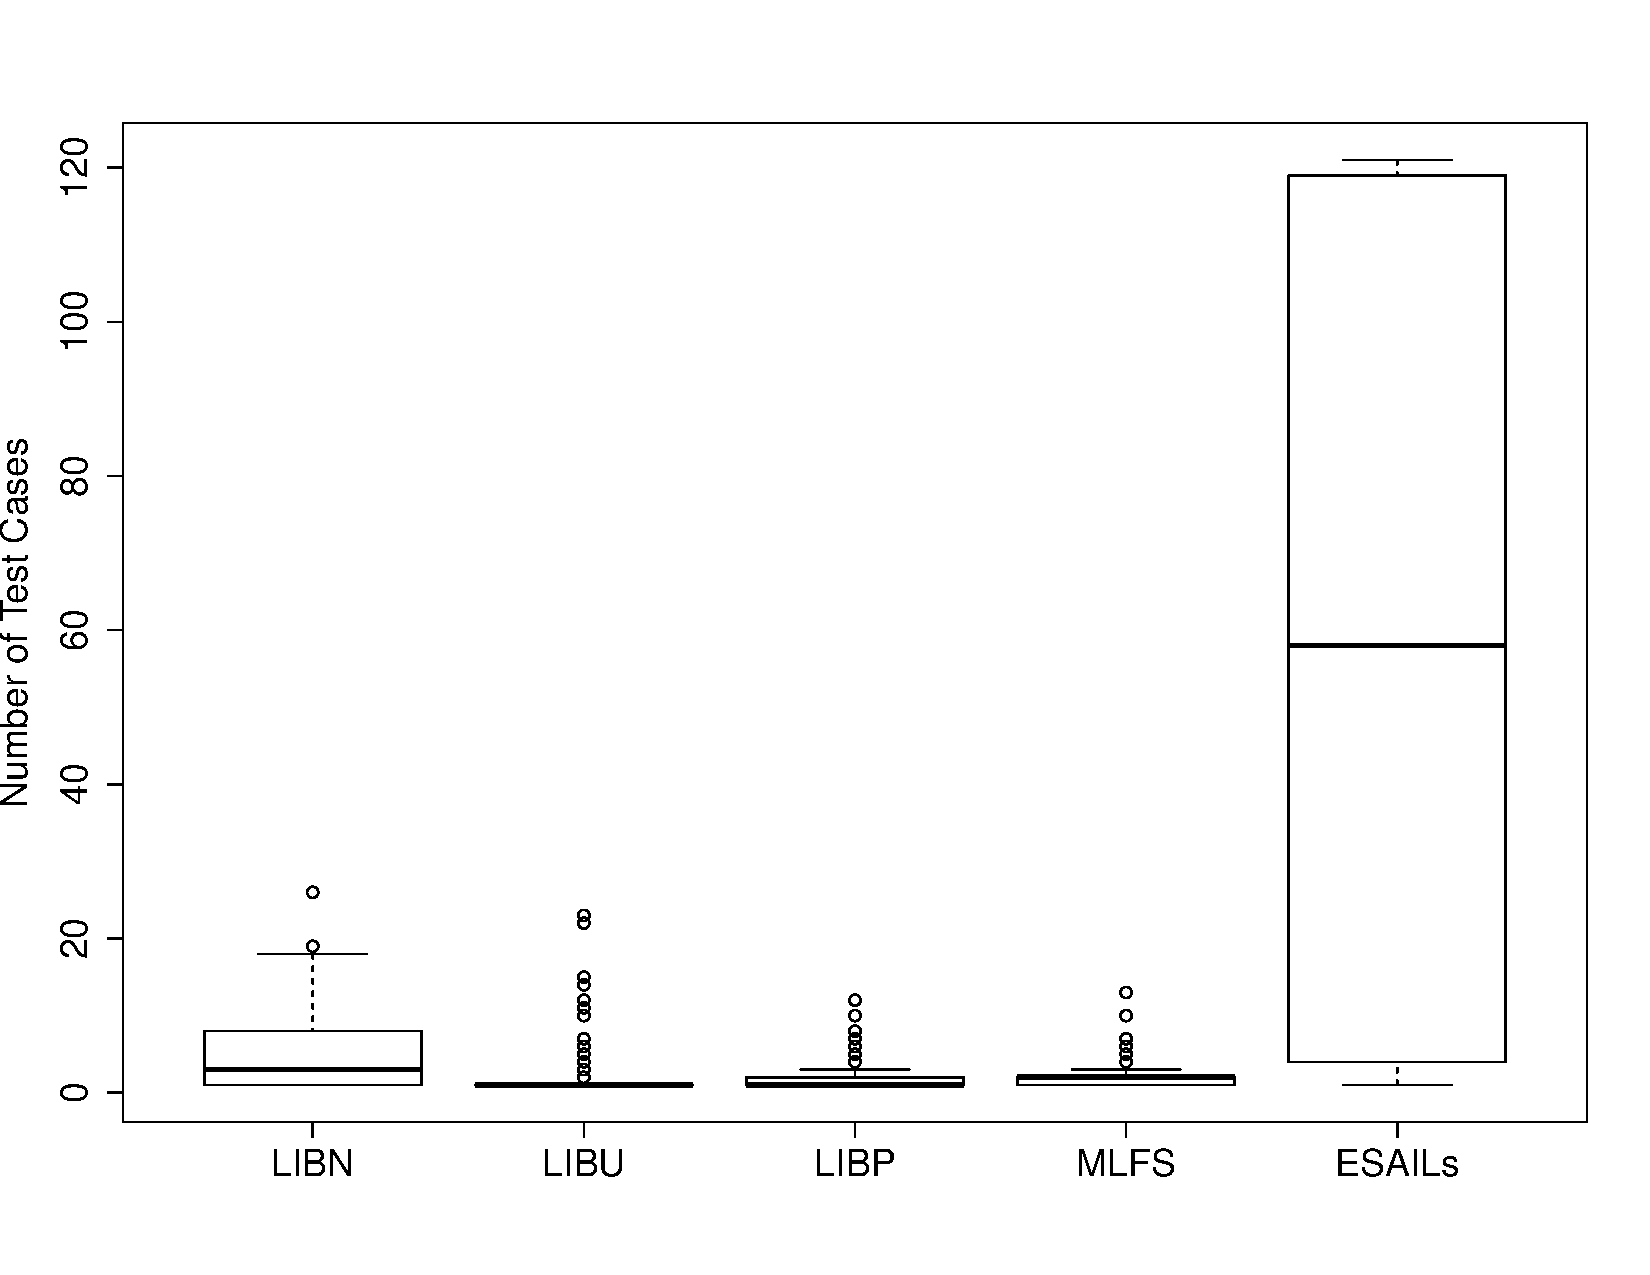
\includegraphics[width=0.8\columnwidth]{images/st_testcases}
\caption{Distribution of test cases exercising each statement.}
\label{fig:tastCaseDist}
\end{center}
\end{figure}

%> min(csp$V1)
%[1] 1
%> min(util$V1)
%[1] 1
%> min(param$V1)
%[1] 1
%> min(mlfs$V1)
%[1] 1
%> min(esail$V1)
%[1] 1
%> max(csp$V1)
%[1] 26
%> max(util$V1)
%[1] 23
%> max(param$V1)
%[1] 12
%> max(mlfs$V1)
%[1] 13
%> max(esail$V1)
%[1] 121
%> mean(csp$V1)
%[1] 4.493617
%> mean(util$V1)
%[1] 1.745416
%> mean(param$V1)
%[1] 2.760691
%> mean(mlfs$V1)
%[1] 2.524808
%> mean(esail$V1)
%[1] 60.96341
%> median(csp$V1)
%[1] 3
%> median(util$V1)
%[1] 1
%> median(param$V1)
%[1] 1
%> median(mlfs$V1)
%[1] 2
%> median(esail$V1)
%[1] 58
%                   [,csp] [,uti] [,para] [,mlf] [,esa]
%[lower whisker,]    1    1    1    1    1
%[lower hinge,]       1    1    1    1    4
%[median,]              3    1    1    2   58
%[upper hinge,]      8    1    2     2   119
%[upper whisker,]   18    1    3    3  121


To address some of our research questions, all the mutants must be executed against the test suite, which is not feasible for the case of \SAIL{}\emph{-CSW} due to its large size and test suite. For this reason, we have identified a subsystem of \SAIL{}\emph{-CSW} (hereafter, \emph{\SAIL{}}$_{S}$) that consists of a set of files, selected by \TWO engineers, that are representative of the different functionalities in \SAIL{}\emph{-CSW}: service/protocol layer functions, critical functions of the satellite implemented in high-level drivers, application layer functions.
Details about $\mathit{\SAIL{}}_{S}$ are reported in Table~\ref{table:caseStudies}.
% \FIXME{note that statement coverage is in line with the whole system.}


Except for \SAIL{}\emph{-CSW}, all subjects
are compiled to generate executables for the development environment OS (Linux); we rely on the Gnu Compiler Collection (GCC)  for Linux X86~\cite{GCC} versions 5.3 and 6.3 for \MLFS{}{} and ONE, respectively. \SAIL{}\emph{-CSW} is compiled with the
LEON/ERC32 RTEMS Cross Compilation System, which includes the GCC C/C++ compiler version 4.4.6 for  RTEMS-4.8 (Sparc architecture)~\cite{RTEMS}.

It is important to note that the technical and test suite characteristics described above are very common in embedded software across many industry domains and cyber-physical systems, thus suggesting our results can be generalizable beyond space software. 

% !TEX root =  ../Main.tex

\begin{table}[tb]
\caption{Descriptions of software components.}
\label{table:caseStudies} 
\scriptsize
\centering
\begin{tabular}{|
@{\hspace{1pt}}p{12mm}
@{\hspace{2pt}}|
@{\hspace{1pt}}>{\raggedleft\arraybackslash}p{8mm}@{\hspace{1pt}}|
@{\hspace{1pt}}>{\raggedleft\arraybackslash}p{18mm}@{\hspace{1pt}}|
@{\hspace{1pt}}>{\raggedleft\arraybackslash}p{20mm}@{\hspace{1pt}}|
@{\hspace{1pt}}>{\raggedleft\arraybackslash}p{24mm}@{\hspace{1pt}}|
p{20mm}|}
\hline
\textbf{Component}&\textbf{LOC}&\textbf{Test suite type}&\textbf{\# Test cases}&\textbf{Statements} \textbf{coverage}\\
\hline
ESAIL& 74155 & System& 384 & 90.38\% \\
ESAIL$_S$& 2235 & System& 384 & 95.36\%\\
LIBGSCSP& 9836 & Integration& 89 & 63.10\%\\
LIBPARAM& 3179 & Integration& 170 & 77.60\%\\
LIBUTIL& 10576 & Unit& 201 & 83.20\%\\
MLFS& 5402 & Unit& 4042 & 100.00\%\\
%MLFS$_V$& 5402 & 4042 & 100.00\%\\
\hline
\end{tabular}

\end{table}

% !TEX root =  ../Main.tex

\begin{table}[tb]
\caption{Generated and compiled mutants per component.}
\label{table:mutants} 
\scriptsize
\begin{tabular}{|
@{\hspace{1pt}}p{12mm}
@{\hspace{2pt}}|
>{\raggedleft\arraybackslash}p{8mm}@{\hspace{1pt}}|
>{\raggedleft\arraybackslash}p{12mm}@{\hspace{1pt}}|
>{\raggedleft\arraybackslash}p{12mm}@{\hspace{1pt}}|
>{\raggedleft\arraybackslash}p{12mm}@{\hspace{1pt}}|
>{\raggedleft\arraybackslash}p{12mm}|}
\hline
\textbf{Component}&\multicolumn{1}{c|}{\textbf{Mutants}}&\multicolumn{1}{c|}{\textbf{Mutants}}&\multicolumn{1}{c|}{\textbf{Mutants}}&\multicolumn{1}{c|}{\textbf{\% of}}&\multicolumn{1}{c|}{\textbf{Mutants}}\\
\textbf{}&\multicolumn{1}{c|}{\textbf{generated}}&\multicolumn{1}{c|}{\textbf{generation}}&\multicolumn{1}{c|}{\textbf{compiled}}&\multicolumn{1}{c|}{\textbf{compiled}}&\multicolumn{1}{c|}{\textbf{compilation}}\\ 
&&\textbf{time} \textbf{(sec)}&&\multicolumn{1}{c|}{\textbf{mutants}}&\multicolumn{1}{c|}{\textbf{time} \textbf{(sec)}}\\ 
\hline
ESAIL& 142763 & 182 &121848& 85.35\% & 151234\\
ESAIL$_S$& & & & &\\
LIBGSCSP& 8666 & 12 &7878&90.91\% & 11425\\
LIBPARAM& 7252 & 7 &6440&88.80\% & 9392\\
LIBUTIL& 22295 & 28 &20268&90.91\% & 30624\\
MLFS& 31526 & 20 &28069&89.03\% &3157\\
%MLFS$_V$& 31526 &T &28069&89.03\% &X\\
\hline
\textbf{Total*}& 212502 & 249 & 184503 &86.82\% &205832\\ 
\hline
\end{tabular}

* We ignore ESAIL$_S$ from the total counting because it is a subset of ESAIL.
\end{table}



\subsection{Setup}
\label{experimnt:setup}

%We should describe the operators used. Potentially could be the superset that is the union of all the operators used in the papers indicated above.
To perform the empirical evaluation, we have implemented the \APPR pipeline in a toolset that is available under the ESA Software Community Licence Permissive~\cite{ESAlicence} at the following URL \textbf{https://faqas.uni.lu/}.
%\footnote{Prior to acceptance, files are shared at {https://dropit.uni.lu/invitations?share=18629a285f6aceacd026}}.
For the implementation of mutation operators, we extended the SRCiror toolset~\cite{hariri2018srciror}.
In our analysis, we consider all the operators reported in Table 1.2 from D2.

Related studies~\cite{zhang2010operator,zhang2013operator} are performed by relying on mutation adequate test suites (i.e., test suites that kill all non-equivalent mutants). 
Such test suites are typically automatically generated using static analysis~\cite{papadakis2012mutation}.
%Since our subject artifacts, as it is common in cyber-physical domains, either require dedicated simulators or include network components, we cannot rely on static analysis to generate mutation adequate test suites. 
%We thus rely on the original test suites provided with the subjects. 
\JMR{3.13}{Since we cannot leverage static analysis to generate mutation adequate test suites (see Section~1.2.1.5 from D2), 
we rely on the original test suites provided with the subjects.}
As a result, to perform our study, we mutate only the statements that are covered by the considered test suites.

\CHANGED{For every subject, we generated mutants by executing the \APPR toolset on Linux OS running on a MacBook Pro with 2,3 GHz 8-Core Intel Core i9. 
Table~\ref{table:mutants} reports, for every subject, the total number of mutants that were generated, their generation time, the number of mutants successfully compiled, the proportion of compiled mutants with respect to the overall number of mutants generated, and the time required to compile mutants using one compiler optimization level only (i.e., the one originally selected by engineers for each subject).
%the default compiler optimization options of the subject.
The generation of mutants is fast, it takes at most {182} seconds on the largest subject (\SAIL{}\emph{-CSW}). On average, across subjects, it takes {11} milliseconds to generate a single mutant. 
The proportion of successfully compiled mutants is large (i.e., 86.82\% overall), though it varies from 85.35\% for \SAIL{}\emph{-CSW} to 90.91\% for \GCSP{} and \UTIL{}.
This proportion is in line with the ones reported in related work, though there is variation. For example, industrial systems 
%that likely contain complex instructions, 
have shown lower success rates (e.g., 81.13\% for safety-critical software components~\cite{Baker2013}) than open source, batch utilities (e.g., 96.30\% for Coreutils~\cite{hariri2016evaluating}).} \REVNOV{PTCR-17}{In the case of compiler warnings, we simply follow the policy configured for the case study. More precisely., in the case of ESAIl and MLFS all the warnings from the compiler lead to a compilation failure. In the case of GSL the compilation process proceeds.}
 
{As shown in Table~\ref{table:mutants}, the time required to compile all the mutants ranges from 3,157 to 151,234 seconds, for an average of 0.96 seconds required to compile a single mutant, across subjects. Because of our selective compilation strategy (see Section~1.2.7 from D2), the time required by our pipeline to compile a single mutant is significantly lower than the one required by state-of-the-art approaches, which is around 4.6 seconds per mutant, even when software components have a lower number of LOC %(i.e., 22,827 LOC)  
than our subjects~\cite{kintis2017detecting}.}

% {The last three columns of Table~\ref{table:mutants} present the number and percentage of mutants successfully compiled, along with the time required to compile all the mutants using the proposed incremental compilation process (Step 3 of \APPR). 
%In total, 86.82\% of the mutants generated among the four case study systems are successfully compiled. 
 



%According to previous research on mutant operator selection, we consider the superset, that is, the union of all the operators defined in the work by Offutt et al.~\cite{offutt1996experimental}, Andrews et al.~\cite{andrews2005mutation} and Kintis et al.~\cite{kintis2017detecting}. The superset consist of the AOR, LCR, ICR, ROR, SDL, UOI, and ABS.
%
%To asses our research questions with the different set of operators considered in the literature, we consider four interleaving subsets of the : the sufficient set (i.e., AOR, LCR, ICR, ROR, SDL, UOI, and ABS),
%the deletion set (i.e., SDL, AOD, LOD, ROD, BOD, and SOD), the extended sufficient set (i.e., all the operators in Table~\ref{table:operators}), and the statement deletion set (i.e., the SDL operator only).  



{To collect the data required to address research questions RQ2 to RQ8, for every subject and unique mutant generated by Step 3, we have executed all the test cases covering the mutated statement. Table~\ref{table:magnitude} provides, for every subject, the overall number of executed test cases and the total execution time required for our experiments. In total, the entire experiment took 1,912,662 minutes (31,878 hours or more than 1300 days). Test  execution time depends on the number of mutants, the number of executed test cases, and the test suite level (e.g., system test suites exercise more complex scenarios than unit or integration test suites).}  
%In our experiments, the execution times of the components tested with unit test suites \FIXME{have the same order of magnitude; indeed, they take between X and Y seconds to execute.}
%In the case of ESAIL, instead, \FIXME{....}}

\CHANGED{To be able to execute test cases for 31,878 hours, we performed our experiments using the HPC cluster of the University of Luxembourg~\cite{HPC}.
The HPC cluster consists of Intel Xeon E5-2680 v4 (2.4 GHz) nodes. To perform our experiments, we tested 100 mutants in parallel, each one on a dedicated node.}

% !TEX root =  ../Main.tex

\begin{table}[tb]
\caption{Experiments magnitude.}
\label{table:magnitude} 
\scriptsize
\centering
\begin{tabular}{|
@{\hspace{1pt}}p{12mm}
@{\hspace{2pt}}|
@{\hspace{1pt}}>{\raggedleft\arraybackslash}p{30mm}@{\hspace{1pt}}|
@{\hspace{1pt}}>{\raggedleft\arraybackslash}p{35mm}@{\hspace{1pt}}|
p{20mm}|}
\hline
\textbf{Case Study}&\textbf{Total test cases executed}&\textbf{Total execution time (minutes)}\\
\hline
%Fabrizio: after removing tests that do not cover the mutants, we should have lower numbers
ESAIL$_S$&  302\,158 & 1\,624\,336\\
LIBGSCSP&  771\,274 & 33\,756\\
LIBPARAM&  1\,094\,800 & 7\,205\\
LIBUTIL&  4\,481\,295 & 57\,732\\
MLFS&  170\,303\,452 & 189\,633\\
%MLFS$_V$& 5402 & 4042 & 100.00\%\\
\hline
\textbf{Total}&  176\,952\,979 & 1\,912\,662\\
\hline
\end{tabular}

\end{table}

In the following sections, we 
%analyze differences in results 
\JMR{3.11}{discuss statistical significance}
using a non-parametric Mann Whitney U-test (with $\alpha$ = 0.05)~\cite{Arcuri:practicalGuide:ICSE:2015}.  We discuss effect size based on Vargha and Delaney’s $A_{12}$ statistics, a non-parametric effect size measure~\cite{VDA,Arcuri:practicalGuide:ICSE:2015}. Based on $A_{12}$, effect size is considered small when $0.56 \le A_{12} < 0.64$, medium when $0.64 \le A_{12} < 0.71$, large when $A_{12} \ge 0.71$. Otherwise the compared samples are considered equivalent, that is to be drawn from the same population~\cite{VDA}.


% % !TEX root =  ../Main.tex

\newcommand{\op}{\mathit{op}}
\newcommand{\ArithmeticSet}{ \texttt{+}, \texttt{-}, \texttt{*}, \texttt{/}, \texttt{\%} }
\newcommand{\LogicalSet}{ \texttt{&&}, \texttt{||} }
\newcommand{\RelationalSet}{ \texttt{>}, \texttt{>=}, \texttt{<}, \texttt{<=}, \texttt{==}, \texttt{!=} }
\newcommand{\BitWiseSet}{ \texttt{\&}, \texttt{|}, \land }
\newcommand{\ShiftSet}{ \texttt{>>}, \texttt{<<} }


\begin{table}[h]
\caption{Implemented set of mutation operators.}
\label{table:operators} 
\centering
\scriptsize
\begin{tabular}{|@{}p{4mm}@{}|@{}p{2cm}@{\hspace{1pt}}|@{}p{11.1cm}@{}|}
\hline
&\textbf{Operator} & \textbf{Description$^{*}$} \\
\hline
\multirow{7}{*}{\rotatebox{90}{\emph{Sufficient Set}}}&ABS               & $\{(v, -v)\}$	\\
\cline{2-3}
&AOR               & $\{(\op_1, op_2) \,|\, \op_1, \op_2 \in \{ \ArithmeticSet \} \land \op_1 \neq \op_2 \} $       \\
&    			  & $\{(\op_1, \op_2) \,|\, \op_1, \op_2 \in \{\texttt{+=}, \texttt{-=}, \texttt{*=}, \texttt{/=}, \texttt{\%} \texttt{=}\} \land \op_1 \neq \op_2 \} $       \\
\cline{2-3}
&ICR               & $\{i, x) \,|\, x \in \{1, -1, 0, i + 1, i - 1, -i\}\}$           \\
\cline{2-3}
&LCR               & $\{(\op_1, \op_2) \,|\, \op_1, \op_2 \in \{ \texttt{\&\&}, || \} \land \op_1 \neq \op_2 \}$            \\
&				  & $\{(\op_1, \op_2) \,|\, \op_1, \op_2 \in \{ \texttt{\&=}, \texttt{|=}, \texttt{\&=}\} \land \op_1 \neq \op_2 \}$            \\
&				  & $\{(\op_1, \op_2) \,|\, \op_1, \op_2 \in \{ \texttt{\&}, \texttt{|}, \texttt{\&\&}\} \land \op_1 \neq \op_2 \}$            \\
\cline{2-3}
&ROR               & $\{(\op_1, \op_2) \,|\, \op_1, \op_2 \in \{ \RelationalSet \}\}$            \\
&				  & $\{ (e, !(e)) \,|\, e \in \{\texttt{if(e)}, \texttt{while(e)}\} \}$ \\
\cline{2-3}
&SDL               & $\{(s, \texttt{remove}(s))\}$            \\
\cline{2-3}
&UOI               & $\{ (v, \texttt{--}v), (v, v\texttt{--}), (v, \texttt{++}v), (v, v\texttt{++}) \}$            \\   
\hline
\hline
\multirow{5}{*}{\rotatebox{90}{\emph{OODL}}}&AOD               & $\{((t_1\,op\,t_2), t_1), ((t_1\,op\,t_2), t_2) \,|\, op \in \{ \ArithmeticSet \} $       \\ 
\cline{2-3}
&LOD               & $\{((t_1\,op\,t_2), t_1), ((t_1\,op\,t_2), t_2) \,|\, op \in \{  \} \}$       \\ 
\cline{2-3}
&ROD               & $\{((t_1\,op\,t_2), t_1), ((t_1\,op\,t_2), t_2) \,|\, op \in \{ \RelationalSet \} \}$       \\ 
\cline{2-3}
&BOD               & $\{((t_1\,op\,t_2), t_1), ((t_1\,op\,t_2), t_2) \,|\, op \in \{ \BitWiseSet \} \}$       \\ 
\cline{2-3}
&SOD               & $\{((t_1\,op\,t_2), t_1), ((t_1\,op\,t_2), t_2) \,|\, op \in \{ \ShiftSet \} \}$       \\ 
%\hline
%COR               & $\{(\op_1, \op_2) \,|\, \op_1, \op_2 \in \{ \texttt{\&\&}, \texttt{||}, \land \} \land \op_1 \neq \op_2 \}$            \\
\hline
\hline
\multirow{3}{*}{\rotatebox{90}{\emph{Other}}}&LVR			& $\{(l_1, l_2) \,|\, (l_1, l_2) \in \{(0,-1), (l_1,-l_1), (l_1, 0), (\mathit{true}, \mathit{false}), (\mathit{false}, \mathit{true})\}\}$\\
&&\\
&&\\
\hline
\end{tabular}

$^{*}$Each pair in parenthesis shows how a program element is modified by the mutation operator. Th eleft element of the pair is replaced with the right element. We follow standard syntax~\cite{kintis2018effective}. Program elements are literals ($l$), integer literals ($i$), boolean expressions ($e$), operators ($\op$), statements ($s$), variables ($v$), and terms ( $t_i$, which might be either variables or literals).
\end{table}

%To generate the mutants, we have extended the SRCIRor mutation testing tool~\cite{hariri2018srciror}. since the original version only implemented the set of operators AOR, LCR, ICR and ROR.

%For each subject of the study we generated mutants by applying the sufficient set of operators. We call this set of mutants complete mutants set.

%We executed the test suites of the case study systems against the complete mutants set. Test execution results let us compute the mutation score of the case study. For each case study, we kept track of the mutants killed by each test case.




%
%To address our research questions considering test suites with different mutation scores for the complete mutants set, for each case study, we derived subsets of the original test suites with different mutation scores. The test suites were randomly derived by randomly selecting test cases till a specific mutation score is reached. We consider test suites with the following mutation scores...

\subsection{RQ1}

% !TEX root =  ../Main.tex
\begin{table*}[htb]
\caption{RQ1. Proportion (\%) of Trivially-Equivalent and Trivially-Redundant Mutants Detected by Compiler Optimizations.}
\label{table:results:compilerOptimizations} 
\tiny
\centering
%\begin{tabular}{|
%p{11mm}|p{6mm}|p{10mm}|
%@{\hspace{2mm}}p{5mm}|p{5mm}|p{5mm}|p{5mm}|p{5mm}|p{5mm}|
%p{6mm}|p{6mm}|p{6mm}|p{6mm}|p{6mm}|p{6mm}|
%}
%\hline
%\textbf{Case} & \textbf{All} & \textbf{Compiled} & \multicolumn{6}{c|}{Equivalent} & \multicolumn{6}{c|}{Redundant} \\
%\textbf{Study}& & 
%&\textbf{O0}&\textbf{O1} & \textbf{O2} & \textbf{O3} & \textbf{Os} & \textbf{Of} 
%&\textbf{O0}&\textbf{O1} & \textbf{O2} & \textbf{O3} & \textbf{Os} & \textbf{Of}
%\\
%\hline
%ESAIL & 142763 & 121848 & 3029 & 8440 & 8520 & 8472 & 8634 & - & 14032 & 21011 & 21768 & 21613 & 21943 & - \\
% &  &  & 2.49  & 6.93  & 6.70  & 6.95  & 7.09  & - & 11.52  & 17.25  & 17.86  & 17.74  & 18.01  & - \\
%LIBUTIL & 22295 & 20268 & 394 & 1277 & 1233 & 1255 & 1247 & 1255 & 2093 & 3092 & 3320 & 3369 & 3383 & 3369 \\
% &  &  & 1.94  & 6.30  & 6.08  & 6.19  & 6.15  & 6.19  & 10.33  & 15.26  & 16.38  & 16.62  & 16.69  & 16.62  \\
%LIBPARAM & 7252 & 6440 & 151 & 428 & 423 & 425 & 436 & 425 & 909 & 1310 & 1346 & 1346 & 1348 & 1346 \\
% &  &  & 2.34  & 6.65  & 6.57  & 6.60  & 6.77  & 6.60 & 14.11  & 20.34  & 20.90  & 20.90  & 20.93  & 20.90  \\
%LIBGSCSP & 8666 & 7878 & 176 & 683 & 511 & 519 & 315 & 336 & 997 & 1756 & 1332 & 1528 & 1690 & 1672 \\
% &  &  & 2.23  & 8.67  & 6.49  & 6.59  & 4.00  & 4.27  & 12.66  & 22.29  & 16.91  & 19.40  & 21.45  & 21.22  \\
%MLFS & 31526 & 28069 & 115 & 230 & 281 & 282 & 307 & 293 & 2386 & 3244 & 3620 & 3628 & 3732 & 3895 \\
% &  &  & 0.41  & 0.82  & 1.00  & 1.00  & 1.09  & 1.04  & 8.50  & 11.55  & 12.90  & 12.93  & 13.30  & 13.88  \\
%\hline
%\textbf{Total}  & 212502 & 184503 & 3773 & 10559 & 10963 & 10557 & 11211 & 2096 & 20479 & 30414 & 31568 & 31800 & 31867 & 10458\\
%&  &  & 2.04  & 5.72  & 5.94  & 5.72  & 6.08  & 1.14  & 11.10  & 16.48  & 17.11  & 17.24  & 17.27  & 5.67  \\
%\hline
%
%\end{tabular}

\begin{tabular}{|
p{11mm}|
@{\hspace{1pt}} >{\raggedleft\arraybackslash}p{9mm}@{\hspace{1pt}}|
@{\hspace{1pt}}>{\raggedleft\arraybackslash}p{10mm}@{\hspace{1pt}}|
@{\hspace{1pt}}>{\raggedleft\arraybackslash}p{8mm}@{\hspace{1pt}}|
>{\raggedleft\arraybackslash}p{5mm}@{\hspace{1pt}}|
>{\raggedleft\arraybackslash}p{8mm}@{\hspace{1pt}}|
 >{\raggedleft\arraybackslash}p{5mm}@{\hspace{1pt}}|
 >{\raggedleft\arraybackslash}p{5mm}@{\hspace{1pt}}|
 >{\raggedleft\arraybackslash}p{5mm}@{\hspace{1pt}}|
 >{\raggedleft\arraybackslash}p{5mm}@{\hspace{1pt}}|
>{\raggedleft\arraybackslash}p{7mm}@{\hspace{1pt}}|
@{\hspace{1pt}} >{\raggedleft\arraybackslash}p{10mm}@{\hspace{1pt}}|
@{\hspace{1pt}} >{\raggedleft\arraybackslash}p{8mm}@{\hspace{1pt}}|
 >{\raggedleft\arraybackslash}p{8mm}@{\hspace{1pt}}|
 >{\raggedleft\arraybackslash}p{6mm}@{\hspace{1pt}}|
 >{\raggedleft\arraybackslash}p{6mm}@{\hspace{1pt}}|
 >{\raggedleft\arraybackslash}p{6mm}@{\hspace{1pt}}|
 >{\raggedleft\arraybackslash}p{6mm}@{\hspace{1pt}}|
 >{\raggedleft\arraybackslash}p{6mm}@{\hspace{1pt}}|
}







\hline
\textbf{Case} & \multicolumn{9}{c|}{\textbf{Equivalent}} & \multicolumn{9}{c|}{\textbf{Redundant}} \\
\textbf{Study}
&\textbf{All}&\textbf{Overall}\textbf{\%}&\textbf{-O0-3}&\textbf{-O0}&\textbf{-O1} & \textbf{-O2} & \textbf{-O3} & \textbf{-Os} & \textbf{-Of} 
&\textbf{All}&\textbf{Overall}\textbf{\%}&\textbf{-O0-3}&\textbf{-O0}&\textbf{-O1} & \textbf{-O2} & \textbf{-O3} & \textbf{-Os} & \textbf{-Of}
\\
\hline
ESAIL &8861&7.27 &7.13&34.18 &95.25 &96.15 &95.61 &97.44 &-&35133&28.83&27.74&39.94 &59.80 &61.96 &61.52 &62.46 &-\\
LIBUTIL &1366&6,74 &6.65&28.84 &93.48 &90.26 &91.87 &91.29 &91.87 &4392&21.67&21.26&47.65 &70.40 &75.59 &76.71 &77.03 &76.71 \\
LIBPARAM &450& 6.99 &6.89&33.56 &95.11 &94.00 &94.44 &96.89 &94.44 &2076&32.24&31.44&43.79 &63.10 &64.84 &64.84 &64.93 &64.84 \\
LIBGSCSP &701&8.90 &8.90&25.11 &97.43 &72.90 &74.04 &44.94 &47.93 &2655&33.70&27.63&37.55 &66.14 &50.17 &57.55 &63.65 &62.98 \\
MLFS &361 &1.29 &1.04&31.86 &63.71 &77.84 &78.12 &85.04 &81.16 &6356&22.64&20.13&37.54 &51.04 &56.95 &57.08 &58.72 &61.28 \\
\hline
\textbf{Total}  &11739&6.36 &6.22&32.14 &89.95 &93.39 &89.93 &95.50 &17.86 &50612&27.43&25.99&40.46 &60.09 &62.37 &62.83 &62.96 &20.66 \\
\hline

\end{tabular}


\end{table*}

\begin{table*}[htb]
\caption{RQ1.  Proportion (\%) of Univocal-Trivially-Equivalent and Univocal-Trivially-Redundant Mutants Detected by Compiler Optimizations.}
\label{table:results:compilerOptimizationsUnivocal} 
\tiny
%\centering
%\begin{tabular}{|
%p{11mm}|p{6mm}|p{10mm}|
%@{\hspace{2mm}}p{6mm}|p{6mm}|p{6mm}|p{6mm}|p{6mm}|p{6mm}|
%p{6mm}|p{6mm}|p{6mm}|p{6mm}|p{6mm}|p{6mm}|
%}
%\hline
%\textbf{Case} & \textbf{All} & \textbf{Compiled} & \multicolumn{6}{c|}{Univocal-Equivalent} & \multicolumn{6}{c|}{Univocal-Redundant} \\
%\textbf{Study}& & 
%&\textbf{O0}&\textbf{O1} & \textbf{O2} & \textbf{O3} & \textbf{Os} & \textbf{Of} 
%&\textbf{O0}&\textbf{O1} & \textbf{O2} & \textbf{O3} & \textbf{Os} & \textbf{Of}
%\\
%\hline
%
%ESAIL & 142763 & 121848 & 0 & 11 & 2 & 47 & 177 & - & 516 & 999 & 1033 & 1175 & 1334 & - \\
%  & & & 0.000  & 0.009  & 0.001  & 0.039  & 0.145  & - & 0.423  & 0.819  & 0.850  & 0.964  & 1.094  & - \\
%LIBUTIL & 22295 & 20268 & 1 & 74 & 2 & 0 & 19 & 0 & 818 & 48 & 4 & 0 & 79 & 4\\
% & & & 0.005  & 0.365  & 0.010  & 0.000  & 0.094  & 0.000  & 4.036  & 0.237  & 0.019  & 0.000  & 0.389  & 0.019  \\
%LIBPARAM & 7252 & 6440 & 0 & 5 & 0 & 0 & 6 & 0 & 20 & 55 & 54 & 0 & 51 & 0\\
% & & & 0.000  & 0.078  & 0.000  & 0.000  & 0.093  & 0.000   & 0.311  & 0.854  & 0.839  & 0.000  & 0.791  & 0.000  \\
%LIBGSCSP & 8666 & 7878 & 0 & 0 & 7 & 0 & 23 & 0 & 1 & 58 & 89 & 0 & 98 & 0\\
% & & & 0.000  & 0.000  & 0.089  & 0.000  & 0.292  & 0.000  & 0.013  & 0.736  & 1.130  & 0.000  & 1.244  & 0.000  \\
%MLFS & 31526 & 28069 & 0 & 6 & 0 & 0 & 39 & 20 & 6 & 60 & 340 & 2 & 443 & 256\\
% & & & 0.000  & 0.021  & 0.000  & 0.000  & 0.139  & 0.071  & 0.021  & 0.214  & 1.211  & 0.007  & 1.578  & 0.912  \\
%\hline
%\textbf{Total}  & 212502 & 184503 & 1 & 96 & 11 & 47 & 264 & 20 & 1046 & 2113 & 529 & 277 & 3114 & 318 \\
% & & & 0.001  & 0.052  & 0.001  & 0.025  & 0.143  & 0.011  & 0.567  & 1.145  & 0.287  & 0.150  & 1.689  & 0.172  \\
%\hline
%
%\end{tabular}

\begin{tabular}{|
p{11mm}|
@{\hspace{1pt}} >{\raggedleft\arraybackslash}p{9mm}@{\hspace{1pt}}|
@{\hspace{1pt}}>{\raggedleft\arraybackslash}p{19mm}@{\hspace{1pt}}|
>{\raggedleft\arraybackslash}p{5mm}@{\hspace{1pt}}|
>{\raggedleft\arraybackslash}p{8mm}@{\hspace{1pt}}|
 >{\raggedleft\arraybackslash}p{5mm}@{\hspace{1pt}}|
 >{\raggedleft\arraybackslash}p{5mm}@{\hspace{1pt}}|
 >{\raggedleft\arraybackslash}p{5mm}@{\hspace{1pt}}|
 >{\raggedleft\arraybackslash}p{5mm}@{\hspace{1pt}}|
>{\raggedleft\arraybackslash}p{7mm}@{\hspace{1pt}}|
@{\hspace{1pt}} >{\raggedleft\arraybackslash}p{19mm}@{\hspace{1pt}}|
 >{\raggedleft\arraybackslash}p{8mm}@{\hspace{1pt}}|
 >{\raggedleft\arraybackslash}p{6mm}@{\hspace{1pt}}|
 >{\raggedleft\arraybackslash}p{6mm}@{\hspace{1pt}}|
 >{\raggedleft\arraybackslash}p{6mm}@{\hspace{1pt}}|
 >{\raggedleft\arraybackslash}p{6mm}@{\hspace{1pt}}|
 >{\raggedleft\arraybackslash}p{6mm}@{\hspace{1pt}}|
}







\hline
\textbf{Case} & \multicolumn{8}{c|}{\textbf{Univocal-Equivalent}} & \multicolumn{8}{c|}{\textbf{Univocal-Redundant}} \\
\textbf{Study}
&\textbf{All}&\textbf{\%} \textbf{of} \textbf{Equivalent}&\textbf{-O0}&\textbf{-O1} & \textbf{-O2} & \textbf{-O3} & \textbf{-Os} & \textbf{-Of} 
&\textbf{All}&\textbf{\%} \textbf{of} \textbf{Redundant}&\textbf{-O0}&\textbf{-O1} & \textbf{-O2} & \textbf{-O3} & \textbf{-Os} & \textbf{-Of}
\\
\hline
ESAIL &237& 2.67&0.00 &4.64 &0.84 &19.83 &\textbf{74.68} &0.00 &5057&14.39&10.20 &19.75 &20.43 &23.24 &\textbf{26.38} &0.00  \\
LIBUTIL &96& 7.03&1.04 &77.08 &2.08 &0.00 &\textbf{19.79} &0.00 &953& 21.70&\textbf{85.83} &5.04 &0.42 &0.00 &8.29 &0.42  \\
LIBPARAM &11 & 2.44&0.00 &45.45 &0.00 &0.00 &\textbf{54.55} &0.00 &180& 8.67&11.11 &\textbf{30.56} &30.00 &0.00 &28.33 &0.00  \\
LIBGSCSP &112 & 15.98&25.11 &\textbf{97.43} &72.90 &74.04 &44.94 &47.93 &429& 16.16&37.55 &\textbf{66.14} &50.17 &57.55 &63.65 &62.98  \\
MLFS &65& 18.01&0.00 &9.23 &0.00 &0.00 &60.00 &\textbf{30.77} &1107& 17.42&0.54 &5.42 &30.71 &0.18 &\textbf{40.02} &23.13 \\
\hline
\textbf{Total}  &521& 4.44&0.19 &18.43 &2.11 &9.02 &\textbf{50.67} &3.84 &7726& 15.27&13.54 &27.35 &6.85 &3.59 &\textbf{40.31} &4.12 \\
\hline

\end{tabular}


\end{table*}


% \begin{table*}[htb]
% \caption{RQ1. Equivalent and Redundant Mutants Detected by Compiler Optimizations.}
% \label{table:results:compilerOptimizations} 
% \tiny
% \begin{tabular}{|
% p{7mm}|p{5mm}|p{7mm}|
% @{\hspace{1mm}}p{4mm}|p{2mm}|p{2mm}|p{2mm}|p{2mm}|p{2mm}|p{2mm}|
% p{2mm}|p{2mm}|p{2mm}|p{2mm}|p{2mm}|p{2mm}|
% p{2mm}|p{2mm}|p{2mm}|p{2mm}|p{2mm}|p{2mm}|
% p{2mm}|p{2mm}|p{2mm}|p{2mm}|p{2mm}|p{2mm}|
% }
% \hline
% \textbf{Case} & \textbf{All} & \textbf{Compiled} & \multicolumn{6}{c|}{Equivalent} & \multicolumn{6}{c|}{Redundant} 
% & \multicolumn{6}{c|}{Univocal-Equivalent}  & \multicolumn{6}{c|}{Univocal-Redundant} \\
% \textbf{Study}&&
% &\textbf{O0}&\textbf{O1} & \textbf{O2} & \textbf{O3} & \textbf{Os} & \textbf{Of} 
% &\textbf{O0}&\textbf{O1} & \textbf{O2} & \textbf{O3} & \textbf{Os} & \textbf{Of}
% &\textbf{O0}&\textbf{O1} & \textbf{O2} & \textbf{O3} & \textbf{Os} & \textbf{Of} 
% &\textbf{O0}&\textbf{O1} & \textbf{O2} & \textbf{O3} & \textbf{Os} & \textbf{Of}
% \\
% ESAIL & 142763 & 121848 & 3029 & 8440 & 8520 & 8472 & 8634 &  & 14032 & 21013 & 21768 & 21613 & 21944 & & 0 & 11 & 2 & 47 & 177 & & 1032 & 1923 & 90 & 240 & 2463 & \\
%  &  &  & 2.49  & 6.93  & 6.70  & 6.95  & 7.09  &  & 11.52  & 17.25  & 17.86  & 17.74  & 18.01  & & 0.00  & 9e-03  & 1.6e-03  & 0.04  & 0.15  &  & 0.85  & 1.58  & 0.07   & 0.2  & 2.02  & \\
% LIBUTIL & 22295 & 20268 & 394 & 1277 & 1233 & 1255 & 1247 & 1255 & 2093 & 3092 & 3319 & 3364 & 3381 & 3368 & 1 & 74 & 2 & 0 & 19 & 0 & 7 & 56 & 7 & 35 & 87 & 62\\
% LIBPARAM & 7252 & 6440 & 151 & 428 & 423 & 425 & 436 & 425 & 909 & 1309 & 1346 & 1346 & 1347 & 1346 & 0 & 5 & 0 & 0 & 6 & 0 & 0 & 16 & 3 & 0 & 23 & 0\\
% LIBGSCSP & 8666 & 7878 & 84 & 184 & 506 & 123 & 587 & 123 & 1059 & 1756 & 1515 & 1849 & 1463 & 1849 & 0 & 0 & 7 & 0 & 23 & 0 & 1 & 58 & 89 & 0 & 98 & 0\\
% MLFS & 31526 & 28069 & 115 & 230 & 281 & 282 & 307 & 293 & 2386 & 3244 & 3620 & 3628 & 3732 & 3895 & 0 & 6 & 0 & 0 & 39 & 20 & 6 & 60 & 340 & 2 & 443 & 256\\
% \hline
% \textbf{Total}  & 212502 & 184503 & 3773 & 10559 & 10963 & 10557 & 11211 & 2096 & 20479 & 30414 & 31568 & 31800 & 31867 & 10458 & 1 & 96 & 11 & 47 & 264 & 20 & 1046 & 2113 & 529 & 277 & 3114 & 318 \\

% %\hline
% %ES\\
% %\hline
% \end{tabular}

% \end{table*}

\begin{table*}[htb]
\caption{RQ1.  Proportion (\%) of Trivially Equivalent/Redundant Mutants Detected per Mutation Operator.}
\label{table:results:compilerOptimizationsProportionOperators} 
\scriptsize
\begin{tabular}{|
p{11mm}|
>{\raggedleft\arraybackslash}p{5mm}@{\hspace{1pt}}|
@{\hspace{1pt}}>{\raggedleft\arraybackslash}p{5mm}@{\hspace{1pt}}|
@{\hspace{1pt}} >{\raggedleft\arraybackslash}p{5mm}@{\hspace{1pt}}|
@{\hspace{1pt}} >{\raggedleft\arraybackslash}p{5mm}@{\hspace{1pt}}|
@{\hspace{1pt}} >{\raggedleft\arraybackslash}p{5mm}@{\hspace{1pt}}|
@{\hspace{1pt}} >{\raggedleft\arraybackslash}p{5mm}@{\hspace{1pt}}|
@{\hspace{1pt}} >{\raggedleft\arraybackslash}p{5mm}@{\hspace{1pt}}|
@{\hspace{1pt}} >{\raggedleft\arraybackslash}p{5mm}@{\hspace{1pt}}|
@{\hspace{1pt}} >{\raggedleft\arraybackslash}p{5mm}@{\hspace{1pt}}|
@{\hspace{1pt}} >{\raggedleft\arraybackslash}p{5mm}@{\hspace{1pt}}|
@{\hspace{1pt}} >{\raggedleft\arraybackslash}p{5mm}@{\hspace{1pt}}|
@{\hspace{1pt}} >{\raggedleft\arraybackslash}p{5mm}@{\hspace{1pt}}|
@{\hspace{1pt}} >{\raggedleft\arraybackslash}p{5mm}@{\hspace{1pt}}|
 >{\raggedleft\arraybackslash}p{5mm}@{\hspace{1pt}}|
@{\hspace{1pt}}>{\raggedleft\arraybackslash}p{5mm}@{\hspace{1pt}}|
@{\hspace{1pt}} >{\raggedleft\arraybackslash}p{5mm}@{\hspace{1pt}}|
@{\hspace{1pt}} >{\raggedleft\arraybackslash}p{5mm}@{\hspace{1pt}}|
@{\hspace{1pt}} >{\raggedleft\arraybackslash}p{5mm}@{\hspace{1pt}}|
@{\hspace{1pt}} >{\raggedleft\arraybackslash}p{5mm}@{\hspace{1pt}}|
@{\hspace{1pt}} >{\raggedleft\arraybackslash}p{5mm}@{\hspace{1pt}}|
@{\hspace{1pt}} >{\raggedleft\arraybackslash}p{5mm}@{\hspace{1pt}}|
@{\hspace{1pt}} >{\raggedleft\arraybackslash}p{5mm}@{\hspace{1pt}}|
@{\hspace{1pt}} >{\raggedleft\arraybackslash}p{5mm}@{\hspace{1pt}}|
@{\hspace{1pt}} >{\raggedleft\arraybackslash}p{5mm}@{\hspace{1pt}}|
@{\hspace{1pt}} >{\raggedleft\arraybackslash}p{5mm}@{\hspace{1pt}}|
@{\hspace{1pt}} >{\raggedleft\arraybackslash}p{5mm}@{\hspace{1pt}}|
}

\hline
\textbf{Case}& \multicolumn{13}{c|}{\textbf{Trivially Equivalent}} &\multicolumn{13}{c|}{\textbf{Trivially Redundant}}\\
\textbf{Study}&
\textbf{ABS}&	\textbf{AOR}&	\textbf{ICR}&	\textbf{LCR}&	\textbf{ROR}&	\textbf{SDL}&	\textbf{UOI}&	\textbf{AOD}&	\textbf{LOD}&	\textbf{ROD}&	\textbf{BOD}&	\textbf{SOD}&	\textbf{LVR}&
\textbf{ABS}&	\textbf{AOR}&	\textbf{ICR}&	\textbf{LCR}&	\textbf{ROR}&	\textbf{SDL}&	\textbf{UOI}&	\textbf{AOD}&	\textbf{LOD}&	\textbf{ROD}&	\textbf{BOD}&	\textbf{SOD}&	\textbf{LVR}\\
\hline
ESAIL&3.65&1.85&6.74&2.09&18.00&1.60&52.34&1.53&0.05&7.64&3.42&0.51&0.59&1.52&6.20&18.79&1.05&23.89&8.04&20.23&4.83&1.06&8.86&2.20&1.96&1.39\\
LIBUTIL&6.66&0.07&3.95&1.24&15.96&7.91&58.86&0.00&0.37&3.81&0.95&0.00&0.22&0.34&7.38&15.64&0.87&30.35&12.61&13.52&1.66&2.66&12.77&0.89&0.52&0.77\\
LIBPARAM&8.89&0.00&0.00&0.22&25.56&6.22&55.33&0.00&0.00&3.56&0.22&0.00&0.00&0.96&3.47&7.95&1.01&36.71&13.58&12.52&1.49&2.46&18.45&0.92&0.00&0.48\\
LIBGSCSP&8.84&0.00&2.28&1.14&17.40&3.14&56.35&0.00&0.14&9.84&0.86&0.00&0.00&2.11&2.37&10.77&1.24&31.45&9.04&23.92&1.69&1.36&13.48&1.58&0.79&0.19\\
MLFS&6.37&0.55&11.63&0.28&27.98&2.77&39.61&0.00&0.00&9.42&1.39&0.00&0.00&5.03&10.12&25.36&0.87&23.77&4.14&6.73&8.51&0.88&9.44&2.33&1.90&0.91\\
\hline
\textbf{Total}&4.59&1.42&6.04&1.81&18.32&2.64&\textbf{53.06}&1.16&0.09&7.22&2.79&0.38&0.47&1.87&6.48&18.47&1.02&25.36&8.23&\textbf{17.83}&4.72&1.25&9.91&2.02&1.68&1.17\\
\hline
\end{tabular}


\end{table*}
% !TEX root =  ../Main.tex

\begin{table}[h]
\caption{RQ1. Compilation Time Required by Compiler Optimization Techniques.}
\label{table:results:compilerOptimizationsTime} 
\tiny
\centering
\begin{tabular}{|
@{\hspace{1pt}}p{11mm}|
@{\hspace{1pt}}>{\raggedleft\arraybackslash}p{7mm}@{\hspace{1pt}}|
>{\raggedleft\arraybackslash}p{7mm}@{\hspace{1pt}}|
>{\raggedleft\arraybackslash}p{7mm}@{\hspace{1pt}}|
>{\raggedleft\arraybackslash}p{7mm}@{\hspace{1pt}}|
>{\raggedleft\arraybackslash}p{7mm}@{\hspace{1pt}}|
>{\raggedleft\arraybackslash}p{7mm}@{\hspace{1pt}}|
 >{\raggedleft\arraybackslash}p{16mm}@{\hspace{1pt}}|
}
\hline
\textbf{Case} & 
\multicolumn{7}{c|}{\textbf{Time required to compile all the mutants(sec)}}\\
\textbf{Study}&
\textbf{O0}&\textbf{O1} & \textbf{O2} & \textbf{O3} & \textbf{Os} & \textbf{Of}
&\textbf{All O* (hours)} 
\\
\hline
ESAIL & 135455 & 132528 & 149088 & 145620 & 151234 & N/A&198\\
LIBUTIL & 25228 & 26914 & 28564 & 30624 & 26845 & 29583 &47\\
LIBPARAM & 9036 & 9246 & 9352 & 9392 & 8794 & 9442 &16\\
LIBGSCSP & 11053 & 11256 & 11079 & 11425 & 10299 & 11424 &18\\
MLFS & 2176 & 2509 & 3157 & 3167 & 3052 & 3164 &5\\
\hline
\textbf{Total}&182948	&182453	&201240	&200228	&200224	&53613 & 284\\
\hline
\end{tabular}

\end{table}

\paragraph{Design and measurements}

RQ1 aims to determine the cost savings provided by 
trivial compiler optimization techniques~\cite{papadakis2015trivial,kintis2017detecting}. To do so, we assess the number of equivalent and duplicate mutants discarded by these techniques and the additional costs introduced by the augmented compilation process. Since the mutants detected by these techniques 
are a subset of 
the overall set of equivalent and duplicate mutants, we refer to them as \INDEX{trivially equivalent} and \INDEX{trivially duplicate} mutants.

For every subject, we compile every mutant six times, each time with a different optimization level enabled. We consider all the available \INDEX{optimization levels} for the GCC compiler, which are \emph{-O0}, \emph{-O1}, \emph{-O2}, \emph{-O3}, \emph{-Os},
% (O2 it includes all O2 optimizations except those increasing executable size), 
and \emph{-Ofast}~\cite{GCCopt}. Level \emph{-O0} indicates that no optimization is applied. Levels \emph{-O1}, \emph{-O2}, \emph{-O3}, and \emph{-Ofast}, in this order, enable an increasing number of optimization options (e.g., level \emph{-Ofast} includes all the optimizations of level \emph{-O3} plus two additional ones, which are \emph{-ffast-math} and \emph{-fallow-store-data-races}). Level \emph{-Os} enables all \emph{-O2} optimizations except those that increase code size. This is the first reported experiment including options \emph{-Os} and \emph{-Ofast} in such an analysis.
 

To identify the most effective compiler optimization level, we consider the percentage of trivially equivalent and trivially duplicate mutants they detect. Also, to discuss how complementary different optimization levels  are and, therefore, whether they should be combined, we report the number of mutants identified as equivalent and duplicate by each compiler optimization only (hereafter called \INDEX{univocal-trivially-equivalent mutants} and \INDEX{univocal-trivially-duplicate mutants}). 

\CHANGED{To further assess the different optimization levels, we analyze the distribution of trivially equivalent and duplicate mutants across the different mutation operators considered in our study.}
% and, furthermore, we manually inspect a randomly selected sample of univocal-equivalent and univocal-duplicate mutants.} 
Last, we compare our results with the ones reported in related work~\cite{papadakis2015trivial}.

\CHANGED{By default, subjects are compiled with  different compiler optimization options, \emph{-Os} for \SAIL{}\emph{-CSW}, \emph{-O2} for \MLFS{}{}, \emph{-O3} for \GCSP{}, \PARAM{}, and \UTIL{}.}
To estimate the costs entailed by the augmented compilation process, we collect, for every subject, the time required for compiling all their mutants with each of the five optimization levels enabled. To compile mutants, we rely on the optimized compilation process implemented in Step 3 of \APPR (see Section~1.2.7 from D2).



\paragraph{Results}

Table~\ref{table:results:compilerOptimizations} provides the results concerning the detection of trivially equivalent and trivially duplicate mutants. We report the total number of such mutants detected for each subject (column \emph{All}), their percentage with respect to the set of mutants successfully compiled (column \emph{Overall \%}), and the percentages obtained with the options included in related work (i.e., by discarding the equivalent and duplicate mutants detected by \emph{-O0}, \emph{-O1}, \emph{-O2}, and \emph{-O3}, reported in column \emph{-O0-3}). 
 The proportion of trivially equivalent mutants detected with optimization levels O0-O3 (6.22\%) is in line with related work~\cite{papadakis2015trivial} (7\%) and the range observed for the different subjects (i.e., 1.04\% to 8.90\%) largely overlaps with the range observed in related work (2\%-10\%). 
 %However, the difference in means with related work is statistically significant and effect size is medium. 
 %Such results can be explained by the fact that, in our context, domain-specific functionalities and code adhering to coding standards are less likely to lead to the generation of trivially equivalent mutants (i.e., any small change in the code tends to impact software behaviour).
 For trivially duplicate mutants, instead, we observe a slightly larger set of duplicate mutants when compared to related work. Optimization levels O0-O3 determine that 25.99\% of the mutants are trivially duplicate, while in related work the average is around 21\%. Finally,  
 optimization levels \emph{-Os} and \emph{-Of} enable the detection of additional trivially equivalent and duplicate mutants, thus leading to an average of \JMR{3.12}{6.36\% and 27.43\% of the mutants being discarded, respectively (see column \emph{Overall \%})}. In particular, \textbf{we observe that the optimization level \emph{-Os}, not evaluated by related work, is the most effective}. Our results confirm the effectiveness of compiler optimizations for removing a significant percentage of equivalent and duplicate mutants.
 
Table~\ref{table:results:compilerOptimizationsUnivocal} provides additional details about the trivially equivalent and duplicate mutants univocally detected by the different optimization options. In total, 4.44\% and 3.34\% of these mutants are univocally detected  by one optimization level (see columns \emph{\% of Equivalent} and \emph{\% of Duplicate}); moreover, since all optimization options contribute to the univocal detection of equivalent and redundant mutants, \textbf{it is preferable to rely on all the available compiler optimization options}. 
\UPDATE{Overall, the most effective optimization option is \emph{-Os}, which detects 50.67\% and 46.34\% of univocal-equivalent and univocal-duplicate mutants, respectively. It is followed by \emph{-O1}, detecting 18.43\% and 10.82\% of such mutants, respectively}. These results suggest that, when the number of compilation runs must be limited, then \emph{-Os} and \emph{-O1} should be prioritized over the other options. This is interesting since \textbf{stronger optimization levels such as \emph{-Ofast} and \emph{-O3} do not contribute more than \emph{-Os} to the detection trivially equivalent and duplicate mutants}. Surprisingly, the optimization level \emph{-O0}, which does not enable any compiler optimization option, can detect trivially equivalent and trivially redundant mutants not detected by other optimization levels. However, this seems to highly depend on the code surrounding the mutated statement. 
\JMR{3.14}{For example, in one \UTIL mutant the optimization level \emph{-O0} detected that \texttt{if ( ptr )} is equivalent to \texttt{if( ptr > NULL )}, with \texttt{ptr} being a pointer, which was not detected with other optimization levels; however, the same instructions are detected as equivalent by other optimization levels when they belong to other functions (i.e., when the code surrounding them is different than the one appearing in the \UTIL mutant).}


To enable further comparison with related work~\cite{kintis2017detecting},
in Table~\ref{table:results:compilerOptimizationsProportionOperators}, we report the proportion of trivially equivalent and  duplicate mutants per mutation operator. The mutation operator causing the largest number of trivially equivalent mutants is UOI (e.g., 
it applies a post-increment operator to the last use of a variable),
%it post-increments the last use of a variable), 
followed by ROR, 
%(e.g., \FIXME{it ... }), 
ROD, 
%(e.g., \FIXME{it ...}), 
and ICR. 
%(e.g., because \FIXME{it ...}). 
Related studies are conducted with a smaller set of operators~\cite{kintis2017detecting}; however, the operators causing the largest numbers of trivially equivalent and duplicate mutants are the same. The main difference with related work~\cite{kintis2017detecting} concerns the ABS operator, which leads to a small set of equivalent mutants in our case, the main reason being that we rely on a definition of the ABS operator that minimizes the number of equivalent mutants by simply inverting the sign of the value instead of using the \emph{abs} function~\cite{Kintis2018}. Indeed, in functions with a positive integer domain, the replacement of a value with its absolute value trivially leads to equivalent mutants. Except for the ABS operator, \textbf{our study confirms the ranking observed in related work} despite different showing proportions. In addition, our results show that \textbf{the nature of the software affects the distribution of equivalent and duplicate mutants across operators}. Indeed, \MLFS{}{}, which focuses on mathematical functions, includes larger proportions of equivalent and duplicate mutants caused by ICR and AOR. In \PARAM{}, which does not deal with mathematical functions, the number of equivalent and duplicate mutants caused by these operators is much smaller. Finally, we notice that the \textbf{SDL and OODL operators lead to a minimal set of trivially equivalent and duplicate mutants, except for ROD}.

% !TEX root =  ../Main.tex

\begin{table*}[htb]
\caption{RQ1.  Proportion (\%) of Trivially Equivalent/Duplicate Mutants Detected per Mutation Operator.}
\label{table:results:compilerOptimizationsProportionOperators} 
\scriptsize
\centering
\begin{tabular}{|
@{\hspace{1pt}}p{9mm}|
@{\hspace{1pt}}>{\raggedleft\arraybackslash}p{5mm}@{\hspace{1pt}}|
@{\hspace{1pt}}>{\raggedleft\arraybackslash}p{5mm}@{\hspace{1pt}}|
@{\hspace{1pt}} >{\raggedleft\arraybackslash}p{5mm}@{\hspace{1pt}}|
@{\hspace{1pt}} >{\raggedleft\arraybackslash}p{5mm}@{\hspace{1pt}}|
@{\hspace{1pt}} >{\raggedleft\arraybackslash}p{5mm}@{\hspace{1pt}}|
@{\hspace{1pt}} >{\raggedleft\arraybackslash}p{5mm}@{\hspace{1pt}}|
@{\hspace{1pt}} >{\raggedleft\arraybackslash}p{5mm}@{\hspace{1pt}}|
@{\hspace{1pt}} >{\raggedleft\arraybackslash}p{5mm}@{\hspace{1pt}}|
@{\hspace{1pt}} >{\raggedleft\arraybackslash}p{5mm}@{\hspace{1pt}}|
@{\hspace{1pt}} >{\raggedleft\arraybackslash}p{5mm}@{\hspace{1pt}}|
@{\hspace{1pt}} >{\raggedleft\arraybackslash}p{5mm}@{\hspace{1pt}}|
@{\hspace{1pt}} >{\raggedleft\arraybackslash}p{5mm}@{\hspace{1pt}}|
@{\hspace{1pt}} >{\raggedleft\arraybackslash}p{5mm}@{\hspace{1pt}}|
 >{\raggedleft\arraybackslash}p{5mm}@{\hspace{1pt}}|
@{\hspace{1pt}}>{\raggedleft\arraybackslash}p{5mm}@{\hspace{1pt}}|
@{\hspace{1pt}} >{\raggedleft\arraybackslash}p{5mm}@{\hspace{1pt}}|
@{\hspace{1pt}} >{\raggedleft\arraybackslash}p{5mm}@{\hspace{1pt}}|
@{\hspace{1pt}} >{\raggedleft\arraybackslash}p{5mm}@{\hspace{1pt}}|
@{\hspace{1pt}} >{\raggedleft\arraybackslash}p{5mm}@{\hspace{1pt}}|
@{\hspace{1pt}} >{\raggedleft\arraybackslash}p{5mm}@{\hspace{1pt}}|
@{\hspace{1pt}} >{\raggedleft\arraybackslash}p{5mm}@{\hspace{1pt}}|
@{\hspace{1pt}} >{\raggedleft\arraybackslash}p{5mm}@{\hspace{1pt}}|
@{\hspace{1pt}} >{\raggedleft\arraybackslash}p{5mm}@{\hspace{1pt}}|
@{\hspace{1pt}} >{\raggedleft\arraybackslash}p{5mm}@{\hspace{1pt}}|
@{\hspace{1pt}} >{\raggedleft\arraybackslash}p{5mm}@{\hspace{1pt}}|
@{\hspace{1pt}} >{\raggedleft\arraybackslash}p{5mm}@{\hspace{1pt}}|
}

\hline
\textbf{}& \multicolumn{13}{c|}{\textbf{Trivially Equivalent}} &\multicolumn{13}{c|}{\textbf{Trivially Duplicate}}\\
\textbf{Subject}&
\textbf{ABS}&	\textbf{AOR}&	\textbf{ICR}&	\textbf{LCR}&	\textbf{ROR}&	\textbf{SDL}&	\textbf{UOI}&	\textbf{AOD}&	\textbf{LOD}&	\textbf{ROD}&	\textbf{BOD}&	\textbf{SOD}&	\textbf{LVR}&
\textbf{ABS}&	\textbf{AOR}&	\textbf{ICR}&	\textbf{LCR}&	\textbf{ROR}&	\textbf{SDL}&	\textbf{UOI}&	\textbf{AOD}&	\textbf{LOD}&	\textbf{ROD}&	\textbf{BOD}&	\textbf{SOD}&	\textbf{LVR}\\
\hline
\mbox{\SAIL{}\emph{-CSW}}
&3.65&1.85&6.74&2.09&18.00&1.60&52.34&1.53&0.05&7.64&3.42&0.51&0.59&1.52&6.20&18.79&1.05&23.89&8.04&20.23&4.83&1.06&8.86&2.20&1.96&1.39\\
\GCSP{}&8.84&0.00&2.28&1.14&17.40&3.14&56.35&0.00&0.14&9.84&0.86&0.00&0.00&2.11&2.37&10.77&1.24&31.45&9.04&23.92&1.69&1.36&13.48&1.58&0.79&0.19\\
\PARAM{}&8.89&0.00&0.00&0.22&25.56&6.22&55.33&0.00&0.00&3.56&0.22&0.00&0.00&0.96&3.47&7.95&1.01&36.71&13.58&12.52&1.49&2.46&18.45&0.92&0.00&0.48\\
\UTIL{}&6.66&0.07&3.95&1.24&15.96&7.91&58.86&0.00&0.37&3.81&0.95&0.00&0.22&0.34&7.38&15.64&0.87&30.35&12.61&13.52&1.66&2.66&12.77&0.89&0.52&0.77\\
\MLFS{}{}&6.37&0.55&11.63&0.28&27.98&2.77&39.61&0.00&0.00&9.42&1.39&0.00&0.00&5.03&10.12&25.36&0.87&23.77&4.14&6.73&8.51&0.88&9.44&2.33&1.90&0.91\\
\hline
\textbf{Total}&4.59&1.42&6.04&1.81&18.32&2.64&\textbf{53.06}&1.16&0.09&7.22&2.79&0.38&0.47&1.87&6.48&18.47&1.02&25.36&8.23&\textbf{17.83}&4.72&1.25&9.91&2.02&1.68&1.17\\
\hline
\end{tabular}


\end{table*}


Finally, to further characterize  the differences across different compiler optimization levels, we provide in Figures~\ref{fig:results:univeq} and~\ref{fig:results:univred}, for each compiler optimization level, the distribution of univocal, trivially equivalent and duplicate mutants across mutation operators. The optimization level \emph{-Os} is more effective in detecting trivially equivalent mutants caused by the ROR operator (a larger number of ROR mutants is associated to \emph{-Os} as captured by the length of the orange bar), while the option \emph{-O1} is more effective in detecting trivially equivalent mutants caused by the UOI operator. Concerning the detection of trivially duplicate mutants (Figure~\ref{fig:results:univred}), \emph{-Os} performs better in detecting the duplicate mutants caused by almost all the operators, except for the ones caused by operators affecting math expressions (i.e., AOR, AOD, and LVR), which are better detected by optimization level \emph{-Ofast}, probably because it includes additional math optimization options.
%  UOI and ROR operators, \FIXME{while \emph{-O0} performs better in detecting duplicate mutants caused by the ROR operator.}

\begin{figure}[tb]
\begin{center}
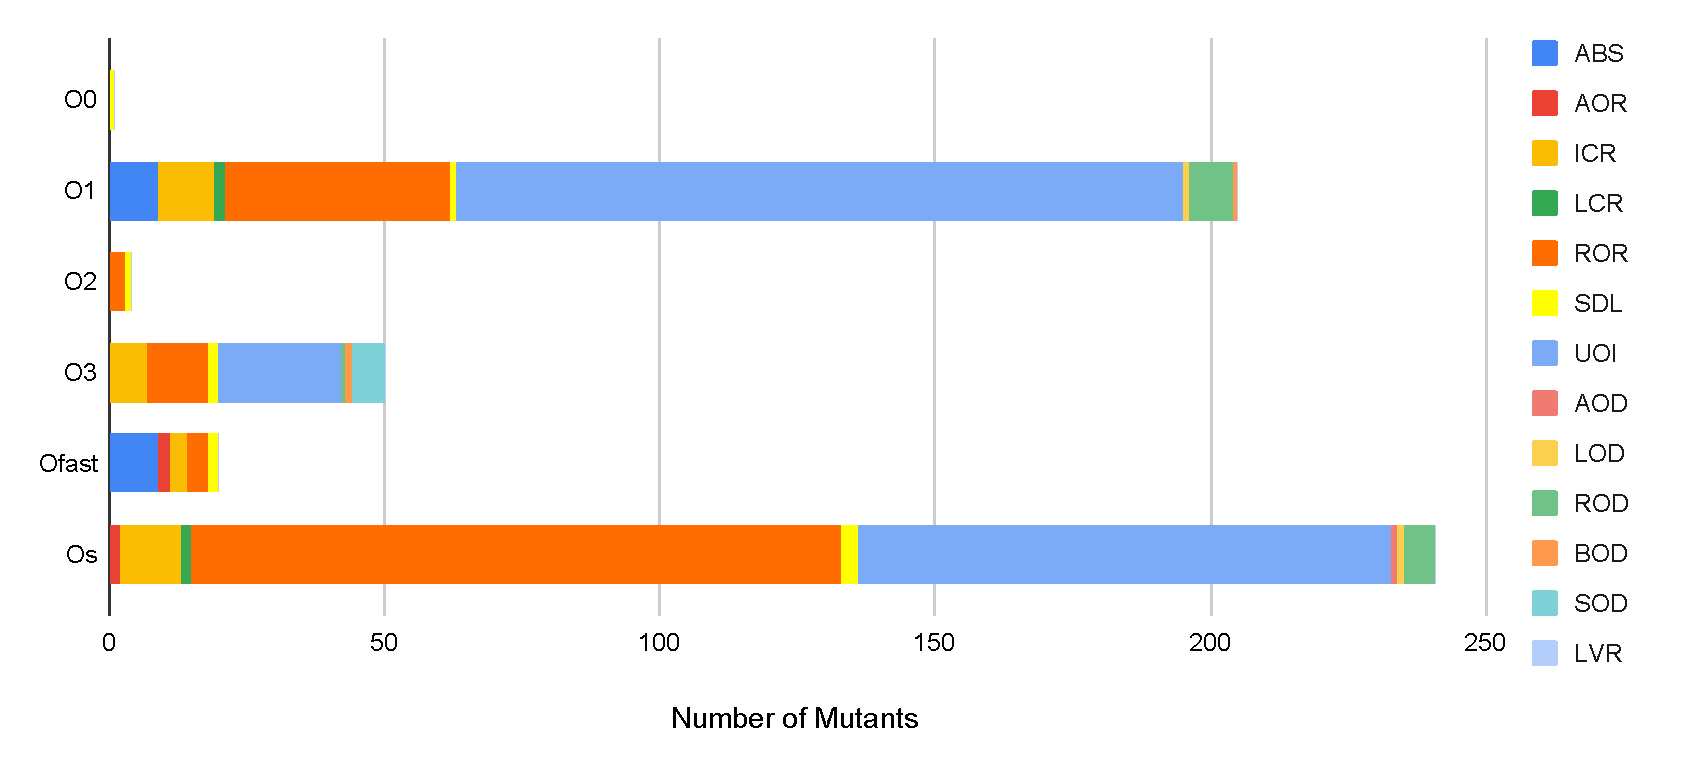
\includegraphics[width=9cm]{images/univ-eq}
\caption{Univocal, Trivially Equivalent Mutants detected by Compiler Optimizations.}
\label{fig:results:univeq}
\end{center}
\end{figure}

\begin{figure}[tb]
\begin{center}
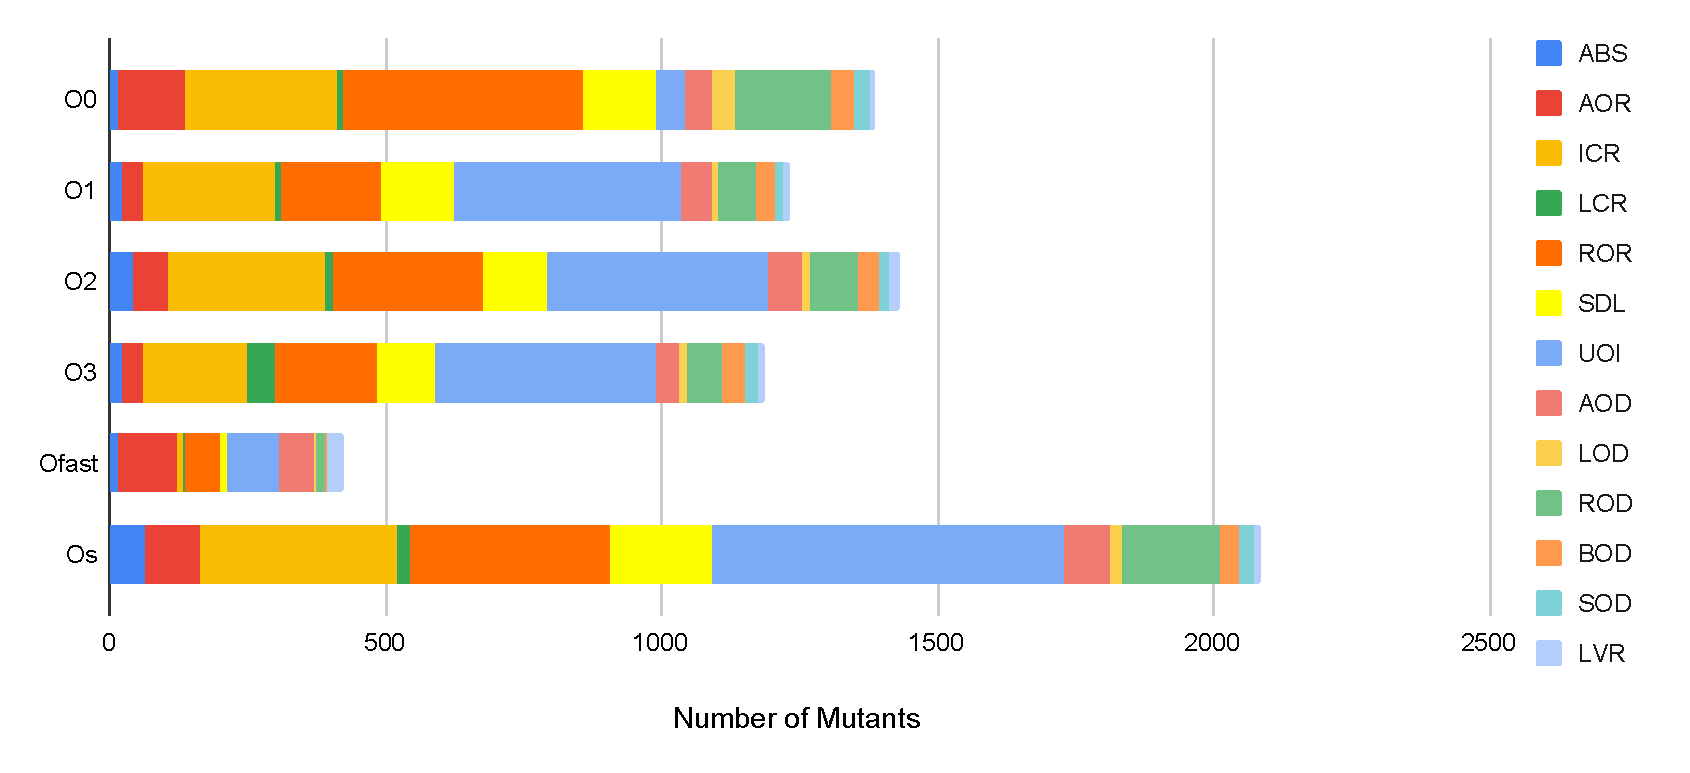
\includegraphics[width=9cm]{images/univ-red}
\caption{Univocal, Trivially Duplicate Mutants detected by Compiler Optimizations.}
\label{fig:results:univred}
\end{center}
\end{figure}




Table~\ref{table:results:compilerOptimizationsTime} provides the time required to compile the artifacts with the different optimization levels. Different from related work, which reports that optimization levels, in the worst case, lead an increase in compilation time by a factor of 5, \textbf{we do not observe a large difference in compilation time among the different optimization levels}. Indeed, in the worst case (i.e., option \emph{-Os}) this factor is $1.1$, an increase of 10\%. This directly results from the \APPR compilation pipeline, which minimizes the number of source files that need to be compiled. If developers can accept a compilation time increased by a factor of 5, as suggested in related work, all the compilation optimization levels can be applied, thus maximizing the number of equivalent and duplicate mutants being detected. In three out of five subjects, it takes less than a day to compile all the mutants with all the available optimization levels, which is acceptable, given the cost saved in subsequent steps. For the cases in which it may take multiple days, our practical solution consists in executing the compilation of the various mutants in parallel (e.g., on Cloud systems); for example, our toolset includes scripts to parallelize mutants compilation on HPC and cloud platforms. In the case of \SAIL{}\emph{-CSW}, the parallel compilation of 142,763 mutants, with the four available compilation options, can be performed in ~90 minutes using 100 nodes.



\subsection{RQ2 - Accuracy of Mutant Sampling Methods}
\label{sec:RQ2}
\paragraph{Design and measurements}


RQ2 aims to investigate  
%the validity of the findings reported by Zhang et al.~\cite{zhang2013operator} and, which concluded that 
to what extent the mutation score computed from a sample of mutants (hereafter, \INDEX{estimated mutation score}) accurately estimates the mutation score of the complete set of mutants (hereafter, \INDEX{actual mutation score}).

In our study, we consider the sampling strategies which are part of \APPR, as justified earlier: \INDEX{proportional uniform sampling}, \INDEX{proportional method-based sampling},  \INDEX{uniform fixed-size sampling}, and \INDEX{uniform FSCI sampling}. 


Because of the complexity and size of space software, combined with its high test execution cost, we are interested in selecting a very small subset of mutants. 
For this reason, 
to evaluate  \INDEX{proportional uniform sampling} and \INDEX{proportional method-based sampling},
we consider sampling ratios ranging from $1\%$ to $10\%$, in steps of $1\%$. Further,
 %to compare our results with those of Zhang et al., 
 we also cover the range 10\% to 100\%, in steps of $10\%$. To evaluate  \INDEX{uniform fixed-size sampling}, consistent with our earlier discussion, we consider a number of mutants in the range 100 to 1000, in steps of $100$.
Finally, to evaluate \INDEX{proportional method-based sampling}, we consider a threshold for the confidence interval (i.e., $T_{\mathit{CI}}$) that ranges from $0.05$ to $0.10$, in steps of $0.01$, with a confidence level of $95\%$, which is a common choice. The experiments conducted to address RQ2 entail the execution of the entire test suite for every sampled mutant. Executions with a prioritized and reduced test suite are addressed in Section~\ref{exp:accuracy:prioritize}. The evaluation of different values for $T_{\mathit{CI}}$ enable us to determine the costs associated with a more accurate estimation of the mutation score, in order to better understand the trade-offs.


We compute the actual mutation score of each system by executing the test suite against all the mutants that were successfully compiled, excluding mutants detected as being equivalent or duplicate by simple compiler optimization techniques (see RQ1). 
For each sampling ratio, to account for randomness,
we repeat the analysis 100 times, i.e., we compute the mutation score 100 times, based on 100 randomly selected subsets of mutants.
%we randomly select 100 subsets of mutants and compute their mutation score. 
Since it is not feasible to test all the mutants generated for \SAIL{}\emph{-CSW}, as discussed above, we focus on $\mathit{\SAIL{}}_{S}$.



%
%Computation in R: 
%X = set of 100 mutation scores
%quantile(X, c(.025, .975))

% s = standard deviation = sd(X)
% true_score = true mutation score
%z.test(X, sigma.x=s, mu=true_score)
%t.test(X, mu=true_score)
%
Our goal is to determine if the estimated mutation score is an accurate estimate of the actual mutation score.
This happens when the estimated mutation score differs from the actual mutation score for less than a small delta (hereafter, accuracy delta, $\delta_{acc}$) for a large percentage of the runs (e.g., 95\%).
We thus study the distribution of the difference between the estimated and actual mutation scores across all runs. More precisely, we estimate the 2.5\% and 97.5\% quantiles\footnote{We rely on linear interpolation using the type 8 
algorithm suggested in Hyndman and Fan~\cite{Hyndman1996}. It does not make assumptions about the underlying distribution.}.
Since these two quantiles delimit 95\% of the population,
we consider the mutation scores to be accurately estimated when they are within a pre-defined small range of the actual score [$-\delta_{acc}$;$+\delta_{acc}$].
In other words, we consider the estimated mutation score to be accurate when 
%the largest absolute value for the two quantiles is below $\delta_{acc}$.
the absolute value of the largest difference between quantiles and the actual score is below $\delta_{acc}$.
Since the range of acceptable mutation score values is small (75\%-100\%, see Section~1.2.1.1 from D2), we decided to use a threshold of 5\%, which is more conservative than that reported in related work ~\cite{gopinath2015hard}. 

Below, we analyze $\delta_{acc}$ for varying sampling rates. To improve readability, we discuss the results concerning the different sampling strategies separately.
% \emph{proportional uniform sampling} and \emph{proportional method-based sampling}.

% (i.e., the max difference between the actual mutation score and either the 2.5\% quantile or the 97.5\% quantile is below 0.01).

%%Since mutants are selected in random order and their result do not depend on the order in which they are executed, they can be treated as  independent from each other. 
%%We thus perform a t-test (alpha = 0.05) to test if the null hypothesis \emph{the mean mutation score of the sampled subset of mutants is equal to the true mutation score}, is rejected.


\paragraph{Results - proportional uniform sampling}

%\begin{figure}[tb]
%\begin{center}
%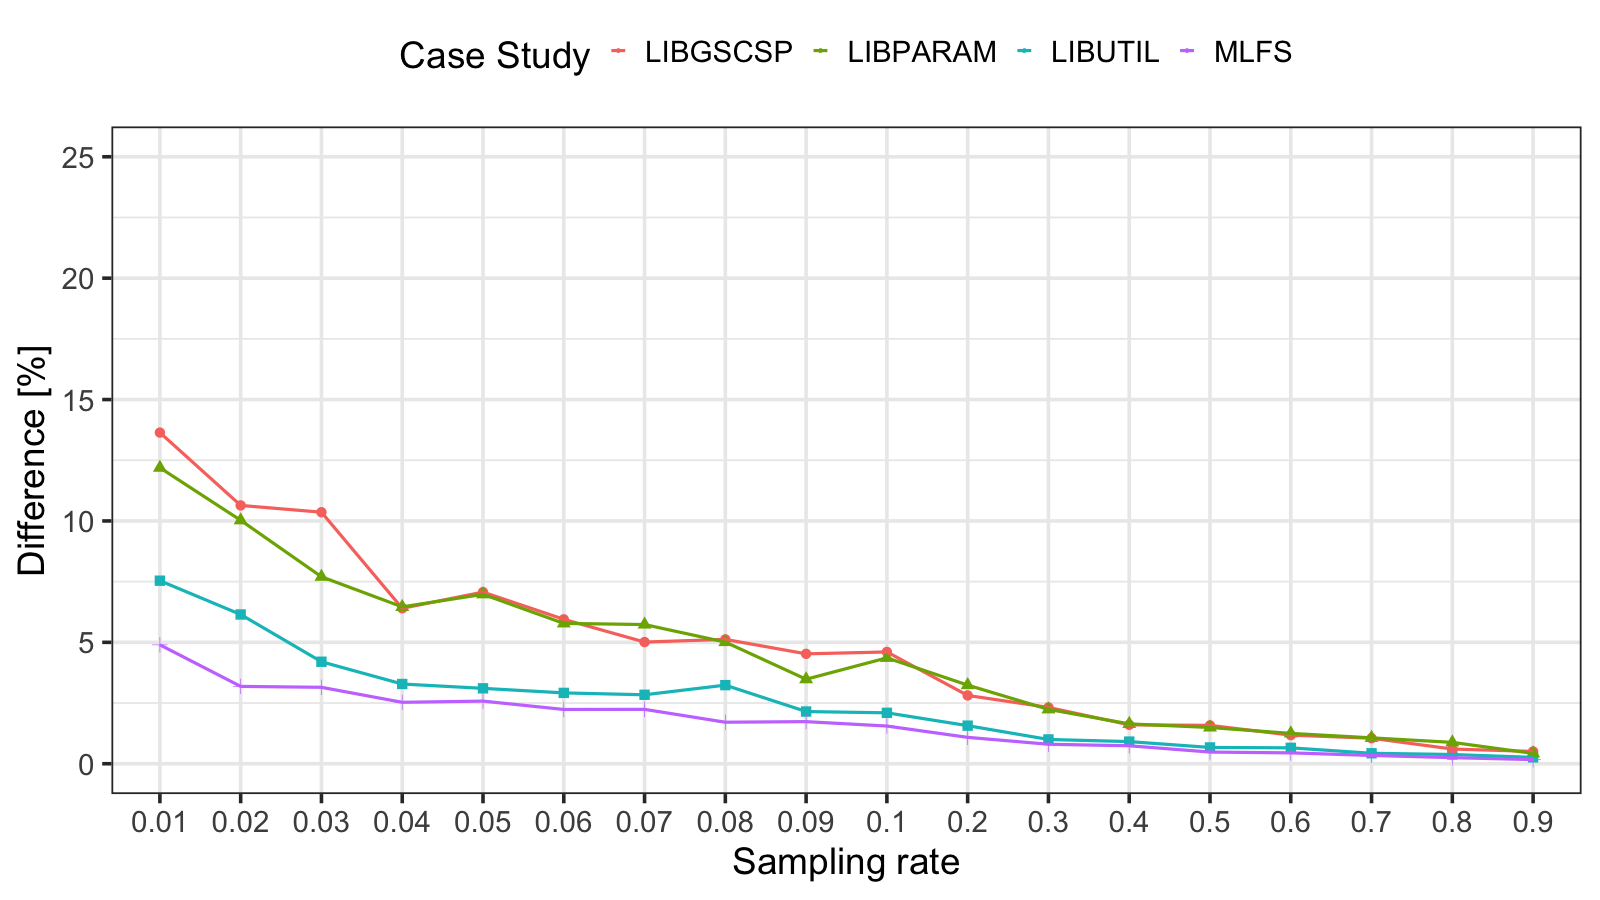
\includegraphics[width=9cm]{images/sampling_regular}
%\caption{Difference between estimated and actual mutation score (i.e., $\delta_{acc}$) for random sampling with different sampling rates.}
%\label{fig:approach}
%\end{center}
%\end{figure}
%
%\begin{figure}[tb]
%\begin{center}
%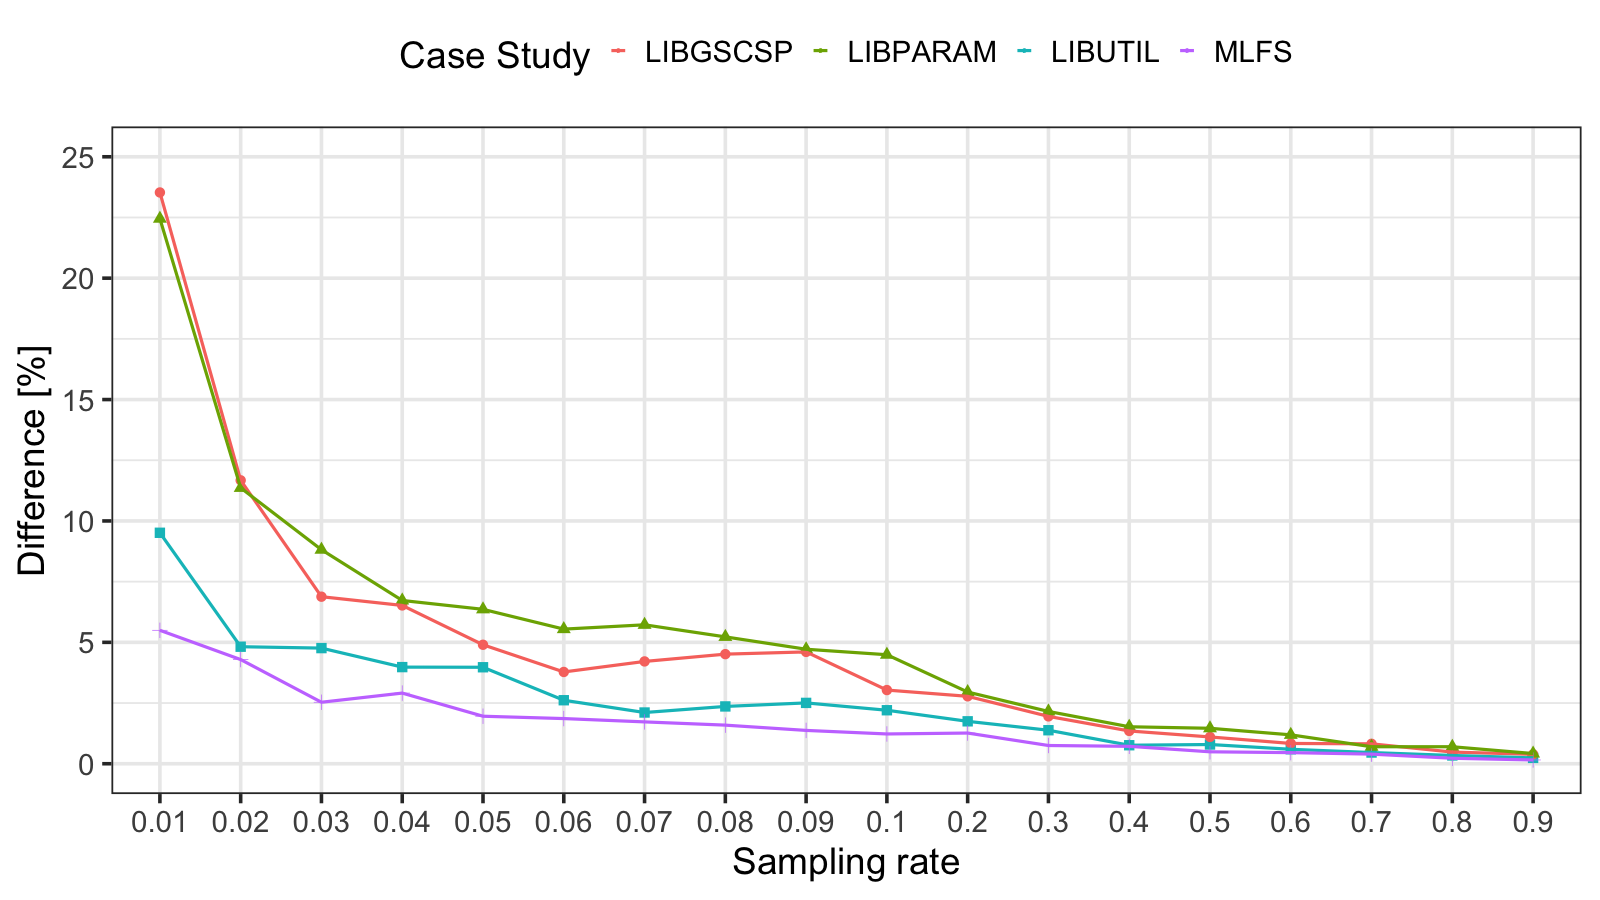
\includegraphics[width=9cm]{images/sampling_func}
%\caption{}
%\label{fig:results:sampling_func}
%\end{center}
%\end{figure}

% !TEX root =  ../Main.tex

\begin{table}[htb]
\caption{Actual mutation scores for artifacts.}
\label{table:results:accuracy:full} 
\scriptsize
\centering
\begin{tabular}{|
@{\hspace{1pt}}p{15mm}|
@{\hspace{1pt}}>{\raggedleft\arraybackslash}p{10mm}@{\hspace{1pt}}|
>{\raggedleft\arraybackslash}p{7mm}@{\hspace{1pt}}|
>{\raggedleft\arraybackslash}p{7mm}@{\hspace{1pt}}|
 >{\raggedleft\arraybackslash}p{25mm}@{\hspace{1pt}}|
}
\hline
\textbf{Case Study}&\textbf{Mutants}&\textbf{Killed}&\textbf{Live}&\textbf{Mutation Score (\%)}\\ 
\hline
$\mathit{ESAIL}_{S}$ &  &  &  &\\
$\mathit{LIBUTIL}$ &20261 & 13590 & 6671 & 71.20 \\
$\mathit{LIBPARAM}$&6435&4291&2144&69.12 \\
$\mathit{LIBGSCSP}$&7878&4905&2973&65.64 \\
$\mathit{MLFS}$&28069&22523&5546&81.80 \\
\hline
\end{tabular}

\end{table}
% !TEX root =  ../Main.tex

\begin{table}[htb]
\caption{RQ2. Accuracy of proportional uniform sampling.}
\label{table:results:accuracy:regSampling} 
\scriptsize
\centering
\begin{tabular}{|
@{\hspace{1pt}}p{5mm}|
@{\hspace{1pt}}>{\raggedleft\arraybackslash}p{7mm}@{\hspace{1pt}}|
>{\raggedleft\arraybackslash}p{5mm}@{\hspace{1pt}}|
>{\raggedleft\arraybackslash}p{6mm}@{\hspace{1pt}}|
 >{\raggedleft\arraybackslash}p{5mm}@{\hspace{1pt}}|
  >{\raggedleft\arraybackslash}p{6mm}@{\hspace{1pt}}|
@{\hspace{1pt}}>{\raggedleft\arraybackslash}p{5mm}@{\hspace{1pt}}|
@{\hspace{1pt}}>{\raggedleft\arraybackslash}p{7mm}@{\hspace{1pt}}|
>{\raggedleft\arraybackslash}p{5mm}@{\hspace{1pt}}|
 >{\raggedleft\arraybackslash}p{8mm}@{\hspace{1pt}}|
  >{\raggedleft\arraybackslash}p{5mm}@{\hspace{1pt}}|
}
\hline
     & \multicolumn{2}{c|}{\textbf{LIBGSCSP}} & \multicolumn{2}{c|}{\textbf{LIBPARAM}} & \multicolumn{2}{c|}{\textbf{LIBUTIL}} & \multicolumn{2}{c|}{\textbf{MLFS}} & \multicolumn{2}{c|}{\textbf{ESAIL}} \\
\hline
\textbf{r=} & \textbf{\#M}&\textbf{$\delta_{acc}$}& \textbf{\#M}&\textbf{$\delta_{acc}$}& \textbf{\#M}&\textbf{$\delta_{acc}$}& \textbf{\#M}&\textbf{$\delta_{acc}$}& \textbf{\#M}&\textbf{$\delta_{acc}$}               \\
\hline
0.01 & 50 & 13.64    			 & 40 & 12.19    			& 146 & 7.54    		& 214 & \textbf{4.90} &   36    & 14.04\\
0.02 & 100 & 10.64    			 & 79 & 10.03    			& 292 & 6.15    		& 428 & \textbf{3.19} &   71    & 11.84\\
0.03 & 150 & 10.36   			 & 118 & 7.70     			& 438 & \textbf{4.20}    & 642 & \textbf{3.15} &   107    & 8.84\\
0.04 & 200 & 6.40     			 & 158 & 6.46     			& 583 & \textbf{3.28}    & 855 & \textbf{2.53} &   142    & 7.92 \\
0.05 & 250 & 7.07     			 & 197 & 6.98     			& 729 & \textbf{3.11}    & 1069 & \textbf{2.58} &  177 & 6.39 \\
0.06 & 299 & 5.95    		 	 & 236 & 5.78     			& 875 & \textbf{2.92}    & 1283 & \textbf{2.24} & 213      &  6.25\\
0.07 & 349 & 5.01     			 & 276 & 5.73     		    & 1021 & \textbf{2.84}    & 1497 & \textbf{2.24} &  248     & 5.20 \\
0.08 & 399 & 5.12    		     & 315 & 5.01 		    	& 1166 & \textbf{3.24}    & 1710 & \textbf{1.71} &  283     & 5.68\\
0.09 & 449 & \textbf{4.53}     	 & 354 & \textbf{3.48}      & 1312 & \textbf{2.15}    & 1924 & \textbf{1.73} &  319     & \textbf{4.55}\\
0.10  & 499 & \textbf{4.61}      & 394 & \textbf{4.36}      & 1458 & \textbf{2.10}    & 2138 & \textbf{1.55} &  354     & \textbf{5.26}\\
0.20  & 997 & \textbf{2.81}      & 787 & \textbf{3.24}      & 2915 & \textbf{1.57}    & 4275 & \textbf{1.09} &    708   & \textbf{3.52}\\
0.30  & 1495 & \textbf{2.32}     & 1180 & \textbf{2.24}     & 4373 & \textbf{1.00}    & 6413 & \textbf{0.80} &  1061 & \textbf{2.56}\\
0.40  & 1993 & \textbf{1.60}     & 1573 & \textbf{1.64}     & 5830 & \textbf{0.91}    & 8550 & \textbf{0.74} &  1415 & \textbf{2.04}\\
0.50  & 2491 & \textbf{1.58}     & 1965 & \textbf{1.49}     & 7287 & \textbf{0.67}    & 10688 & \textbf{0.48} & 1768  & \textbf{1.50}\\
0.60  & 2990 & \textbf{1.18}     & 2358 & \textbf{1.25}     & 8745 & \textbf{0.66}    & 12825 & \textbf{0.45} & 2122  & \textbf{1.28}\\
0.70  & 3488 & \textbf{1.05}     & 2750 & \textbf{1.07}     & 10202 & \textbf{0.43}    & 14963 & \textbf{0.34} & 2476   & \textbf{1.16}\\
0.80  & 3986 & \textbf{0.61}     & 3143 & \textbf{0.88}     & 11660 & \textbf{0.38}    & 17100 & \textbf{0.25} & 2829   & \textbf{0.92}\\
0.90  & 4484 & \textbf{0.51}     & 3534 & \textbf{0.43}     & 13117 & \textbf{0.26}   & 19238 & \textbf{0.17} & 3183& \textbf{0.55}\\
\hline 
\end{tabular}

Note: \#M, number of mutants. Accurate results (i.e., $\delta_{acc} \le 5\%$) are in bold.
\end{table}

\begin{table}[htb]
\caption{RQ2. Accuracy of proportional method-based sampling.}
\label{table:results:accuracy:methodBased} 
\scriptsize
\centering
\begin{tabular}{|
@{\hspace{1pt}}p{5mm}|
@{\hspace{1pt}}>{\raggedleft\arraybackslash}p{7mm}@{\hspace{1pt}}|
>{\raggedleft\arraybackslash}p{5mm}@{\hspace{1pt}}|
>{\raggedleft\arraybackslash}p{6mm}@{\hspace{1pt}}|
 >{\raggedleft\arraybackslash}p{5mm}@{\hspace{1pt}}|
  >{\raggedleft\arraybackslash}p{6mm}@{\hspace{1pt}}|
@{\hspace{1pt}}>{\raggedleft\arraybackslash}p{5mm}@{\hspace{1pt}}|
@{\hspace{1pt}}>{\raggedleft\arraybackslash}p{7mm}@{\hspace{1pt}}|
>{\raggedleft\arraybackslash}p{5mm}@{\hspace{1pt}}|
 >{\raggedleft\arraybackslash}p{8mm}@{\hspace{1pt}}|
  >{\raggedleft\arraybackslash}p{5mm}@{\hspace{1pt}}|
}
\hline
     & \multicolumn{2}{c|}{\textbf{LIBGSCSP}} & \multicolumn{2}{c|}{\textbf{LIBPARAM}} & \multicolumn{2}{c|}{\textbf{LIBUTIL}} & \multicolumn{2}{c|}{\textbf{MLFS}} & \multicolumn{2}{c|}{\textbf{ESAIL}} \\
\hline
\textbf{r=} & \textbf{\#M}&\textbf{$\delta_{acc}$}& \textbf{\#M}&\textbf{$\delta_{acc}$}& \textbf{\#M}&\textbf{$\delta_{acc}$}& \textbf{\#M}&\textbf{$\delta_{acc}$}& \textbf{\#M}&\textbf{$\delta_{acc}$}               \\
\hline
0.01 & 19 & 23.53    			 & 15 & 22.45    			& 111 & 9.51    		 & 232 & 5.50 &  33& 13.84\\
0.02 & 75 & 11.67    			 & 77 & 11.36    			& 250 & \textbf{4.82}    & 447 & \textbf{4.29} &64& 16.18\\
0.03 & 131 & 6.88    			 & 120 & 8.82    			 & 422 & \textbf{4.76}   & 661 & \textbf{2.53} &104   &8.63\\
0.04 & 194 & 6.52    			 & 165 & 6.73    			 & 564 & \textbf{3.98}   & 881 & \textbf{2.91} &137 &9.93\\
0.05 & 258 & \textbf{4.90}     & 208 & 6.36     			& 731 & \textbf{3.97}    & 1094 & \textbf{1.96} &178   &6.84\\
0.06 & 312 & \textbf{3.78}     & 254 & 5.54     			& 905 & \textbf{2.62}    & 1306 & \textbf{1.86} &223& 6.18\\
0.07 & 368 & \textbf{4.21}     & 290 & 5.72     			& 1045 & \textbf{2.11}    & 1517 & \textbf{1.72} &254& 5.72\\
0.08 & 417 & \textbf{4.51}     & 335 & 5.22     			& 1197 & \textbf{2.36}    & 1733 & \textbf{1.59} & 287&\textbf{4.67}\\
0.09 & 466 & \textbf{4.61}     & 378 & \textbf{4.72}    	 & 1353 & \textbf{2.51}    & 1942 & \textbf{1.37} & 331      &\textbf{4.59}\\
0.1  & 515 & \textbf{3.03}     & 413 & \textbf{4.49}     	& 1512 & \textbf{2.20}    & 2159 & \textbf{1.23} &364&\textbf{3.87}\\
0.2  & 1030 & \textbf{2.78}     & 811 & \textbf{2.95}     	& 2963 & \textbf{1.75}    & 4295 & \textbf{1.26} & 721  & \textbf{2.95}\\
0.3  & 1523 & \textbf{1.95}     & 1210 & \textbf{2.15}     & 4446 & \textbf{1.38}    & 6430 & \textbf{0.75} & 1079&\textbf{2.76}\\
0.4  & 2045 & \textbf{1.35}     & 1605 & \textbf{1.52}     & 5942 & \textbf{0.76}    & 8576 & \textbf{0.72} & 1432&\textbf{1.81}\\
0.5  & 2518 & \textbf{1.10}     & 1985 & \textbf{1.46}     & 7361 & \textbf{0.79}    & 10702 & \textbf{0.49} & 1779&\textbf{1.42}\\
0.6  & 3035 & \textbf{0.84}     & 2395 & \textbf{1.19}     & 8853 & \textbf{0.60}    & 12863 & \textbf{0.46} & 2139&\textbf{1.22}\\
0.7  & 3550 & \textbf{0.82}     & 2791 & \textbf{0.70}     & 10334 & \textbf{0.46}    & 15007 & \textbf{0.40} & 2494&\textbf{1.03}\\
0.8  & 4027 & \textbf{0.48}     & 3178 & \textbf{0.70}     & 11779 & \textbf{0.34}    & 17134 & \textbf{0.23} & 2849&\textbf{0.86}\\
0.9  & 4527 & \textbf{0.39}     & 3574 & \textbf{0.42}     & 13228 & \textbf{0.24}    & 19272 & \textbf{0.16} & 3202&\textbf{0.62}\\
\hline
\end{tabular}

Note: \#M, number of mutants. Accurate results (i.e., $\delta_{acc} \le 5\%$) are in bold.
\end{table}




Table~\ref{table:results:accuracy:full} reports on the mutation scores obtained with the entire test suite for all subjects. 
As expected, the best mutation score is obtained for \MLFS{}{}, whose test suite achieves MC/DC coverage. \REVNOV{PTCR-20}{In this project, based on related work, we assume a good quality test suite to have a mutation score above 75\%. However, the objective of this report is not to evaluate the quality of the provided test suites based on the observed mutation score but to evaluate the approach for estimating the mutation score. A discussion of of the quality of the provided test suites based on the mutation score is an activity that might be left for later stages when the mutation testing approach is completed and partners had time to inspect live mutants. Indeed,
 there are a number of factors that affect the computed mutation score; for example, the presence of equivalent mutants lead to live mutants and, consequently, make the mutation score (erroneously) low. The inspection of equivalent mutants for the case studies is till ongoing, at this stage. Also, the reasons for not achieving a high mutation score may vary from case study to case study and needs an in depth investigation. For example, for GSL case studies, this seems to be related to a number of off-the-shelf components integrated in the source of the system. Such off-the-shelf-components are not expected to be tested by the test suite. A mutation score based on only non off-the-shelf-components will be computed in later stages of the project.}

%Figure~\ref{fig:results:accuracy:sampling}  reports a plot with the maximum absolute value of the difference...
Table~\ref{table:results:accuracy:regSampling} provides accuracy results (column $\delta_{acc}$) for proportional uniform sampling for a range of sampling rates~($r$). 
To enable comparisons across sampling methods, Column \emph{\#M} reports the number of mutants sampled for each sampling rate.
As expected, a larger sampling rate leads to more accurate results (i.e., low $\delta_{acc}$). 
We notice that for test suites that ensure MC/DC coverage (i.e., \MLFS{}{}), even a very small sampling ratio (i.e., 0.01) guarantees a $\delta_{acc}$ below 5\%. However, to achieve an accurate mutation score estimate across all subjects, a minimum sampling rate of 0.09 is required.

%Table~\ref{table:results:accuracy:sampling} reports, for every case study system, sampling strategy, and sampling ratio, the max difference between the actual mutation score and either the 2.5\%/97.5\% quantile.

%\FIXME{... We cannot go much below 5\%, but in certain systems 5\% is still a lot.}

In addition, we observe that, for $r=0.09$, the worst results (highest deltas) are observed for smaller projects, which indicates that \textbf{the estimation accuracy may not depend on the percentage of sampled mutants but on the size of the sample}; indeed, for most of the subjects, accurate results \CHANGED{(i.e., $\delta_{acc} < 5\%$)} are obtained with a number of mutants between 350 and 450. This aspect is further studied when considering  \INDEX{uniform fixed-size sampling} and \INDEX{uniform FSCI sampling}.

\paragraph{Results - proportional method-based sampling}

Table~\ref{table:results:accuracy:methodBased} shows the accuracy results for proportional method-based sampling. 
Interestingly, for two subjects (i.e., \GCSP{} and \UTIL{}), proportional method-based sampling leads to accurate estimates of the mutation score with a lower number of mutants than proportional uniform sampling (i.e., around 250).
However, to achieve accurate results with all subjects, we need a minimal sampling rate of $r=0.09$, as for proportional uniform sampling, which, in the case of method-based sampling, leads to a slightly higher number of mutants. For this reason, we do not see any benefit in using method-based sampling.




\paragraph{Results - uniform fixed-size sampling, uniform FSCI sampling}

%\begin{figure}[tb]
%\begin{center}
%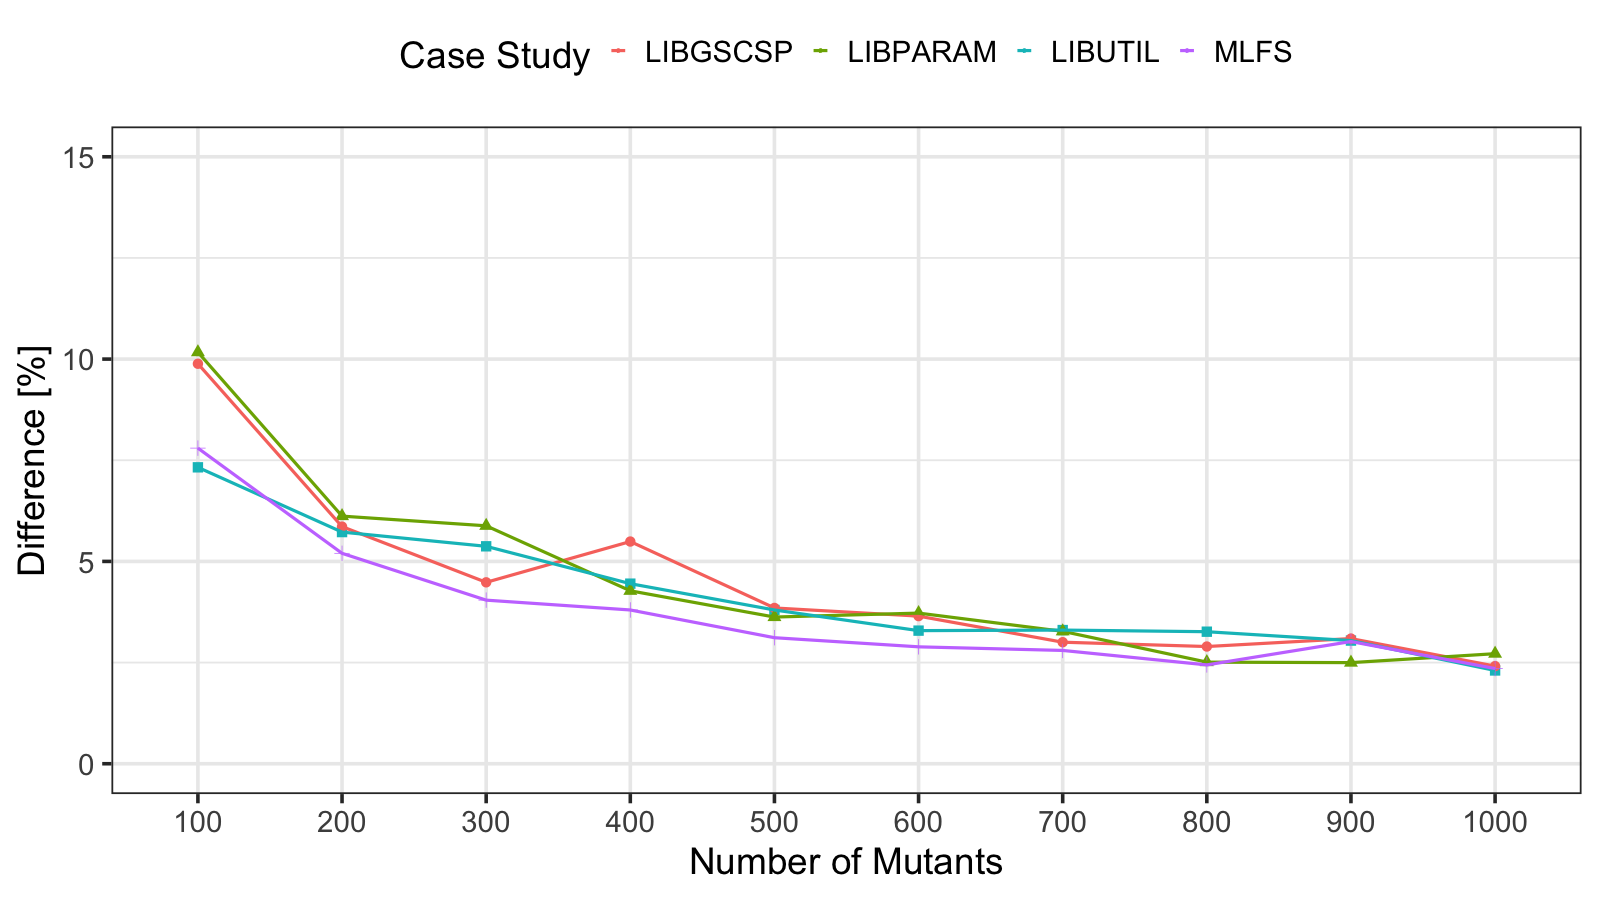
\includegraphics[width=6cm]{images/sampling_fixed}
%\caption{}
%\label{fig:results:fixedNumberOfMutants}
%\end{center}
%\end{figure}
% !TEX root =  ../Main.tex

\begin{table*}[htb]
\caption{RQ2. Accuracy with uniform fixed-size sampling and uniform FSCI sampling. }
\label{table:results:accuracy:FSCI:sampling} 
\scriptsize
\centering
\begin{tabular}{|
>{\raggedleft\arraybackslash}p{10mm}@{\hspace{1pt}}|
>{\raggedleft\arraybackslash}p{5mm}@{\hspace{1pt}}|
p{12mm}@{\hspace{1pt}}|
>{\raggedleft\arraybackslash}p{10mm}@{\hspace{1pt}}|
>{\raggedleft\arraybackslash}p{5mm}@{\hspace{1pt}}|
p{12mm}@{\hspace{1pt}}|
>{\raggedleft\arraybackslash}p{10mm}@{\hspace{1pt}}|
>{\raggedleft\arraybackslash}p{5mm}@{\hspace{1pt}}|
p{12mm}@{\hspace{1pt}}|
>{\raggedleft\arraybackslash}p{10mm}@{\hspace{1pt}}|
>{\raggedleft\arraybackslash}p{5mm}@{\hspace{1pt}}|
p{12mm}@{\hspace{1pt}}|
>{\raggedleft\arraybackslash}p{10mm}@{\hspace{1pt}}|
>{\raggedleft\arraybackslash}p{5mm}@{\hspace{1pt}}|
p{12mm}@{\hspace{1pt}}|
}
\hline
\multicolumn{3}{|c|}{\textbf{LIBGSCSP}}      & \multicolumn{3}{c|}{\textbf{LIBPARAM}}      & \multicolumn{3}{c|}{\textbf{LIBUTIL}}       & \multicolumn{3}{c|}{\textbf{MLFS}}          & \multicolumn{3}{c|}{\textbf{ESAIL}}       \\
\hline
\textbf{\#Mutants} & $\delta_{acc}$ & \textbf{Method}   & \textbf{\#Mutants} & $\delta_{acc}$ & \textbf{Method}   & \textbf{\#Mutants} & $\delta_{acc}$ & \textbf{Method}   & \textbf{\#Mutants} & $\delta_{acc}$ & \textbf{Method}   & \textbf{\#Mutants} & $\delta_{acc}$ & \textbf{Method} \\
\hline
100       & 9.88       & FIXED    & 100       & 10.17      & FIXED    & 100       & 7.32       & FIXED    & 100       & 7.80       & FIXED    &  100         &     8.89       &   FIXED     \\
200       & 5.86       & FIXED    & 200       & 6.12       & FIXED    & 200       & 5.73       & FIXED    & 200       & 5.20       & FIXED    &   200        &      6.14      &   FIXED     \\
300       & \textbf{4.48}       & FIXED    & 300       & 5.88       & FIXED    & 300       & 5.37       & FIXED    & 248       & \textbf{4.56}       & CI 0.1  &    300       &      5.53      &    FIXED    \\
364       & \textbf{4.42}       & FSCI 0.1  & 346       & \textbf{4.26}       & FSCI 0.1  & 333       & \textbf{4.73}       & FSCI 0.1  & 300       & \textbf{4.04}       & FIXED    &   366        &     \textbf{3.92}       &    FSCI 0.1    \\
400       & \textbf{5.49}       & FIXED    & 400       & \textbf{4.27}       & FIXED    & 400       & \textbf{4.45}       & FIXED    & 302       & \textbf{4.64}       & FSCI 0.09 &     400      &     \textbf{4.52}       &    FIXED    \\
447       & \textbf{3.70}       & FSCI 0.09 & 425       & \textbf{3.79}       & FSCI 0.09 & 409       & \textbf{4.08}       & FSCI 0.09 & 379       & \textbf{4.01}       & FSCI 0.08 &   449        &    \textbf{3.66}     &   FSCI 0.09    \\
500       & \textbf{3.85}       & FIXED    & 500       & \textbf{3.63}       & FIXED    & 500       & \textbf{3.80}       & FIXED    & 400       & \textbf{3.80}       & FIXED    &   500      &      \textbf{4.08}      &   FIXED     \\
564       & \textbf{3.53}       & FSCI 0.08 & 536       & \textbf{3.75}       & FSCI 0.08 & 514       & \textbf{3.94}       & FSCI 0.08 & 490       & \textbf{3.90}       & FSCI 0.07 &    567       &  \textbf{3.03}   &  FSCI 0.08      \\
600       & \textbf{3.65}       & FIXED    & 600       & \textbf{3.72}       & FIXED    & 600       & \textbf{3.29}       & FIXED    & 500       & \textbf{3.11}       & FIXED    &     600      &  \textbf{3.73}          &     FIXED   \\
700       & \textbf{3.00}       & FIXED    & 696       & \textbf{2.89}       & FSCI 0.07 & 668       & \textbf{3.99}       & FSCI 0.07 & 600       & \textbf{2.89}       & FIXED    &     700      &      \textbf{3.01}      &    FIXED    \\
734       & \textbf{3.62}       & FSCI 0.07 & 700       & \textbf{3.27}       & FIXED    & 700       & \textbf{3.30}       & FIXED    & 667       & \textbf{2.78}       & FSCI 0.06 &     738      &      \textbf{2.77}      &    FSCI 0.07    \\
800       & \textbf{2.90}       & FIXED    & 800       & \textbf{2.51}       & FIXED    & 800       & \textbf{3.26}       & FIXED    & 700       & \textbf{2.80}       & FIXED    &     800      &  \textbf{2.55}          &    FIXED    \\
900       & \textbf{3.09}       & FIXED    & 900       & \textbf{2.50}       & FIXED    & 900       & \textbf{3.04}       & FIXED    & 800       & \textbf{2.44}       & FIXED    &     900      &  \textbf{2.37}          &    FIXED    \\
994       & \textbf{3.00}       & FSCI 0.06 & 945       & \textbf{2.42}       & FSCI 0.06 & 906       & \textbf{3.28}       & FSCI 0.06 & 900       & \textbf{3.02}       & FIXED    &  998         &  \textbf{2.65}         &   FSCI 0.06     \\
1000      & \textbf{2.41}       & FIXED    & 1000      & \textbf{2.72}       & FIXED    & 1000      & \textbf{2.31}       & FIXED    & 960       & \textbf{2.31}       & FSCI 0.05 & 1000     &  \textbf{2.96}          &   FIXED     \\
1422      & \textbf{2.44}       & FSCI 0.05 & 1352      & \textbf{1.93}       & FSCI 0.05 & 1298      & \textbf{2.72}       & FSCI 0.05 & 1000      & \textbf{2.35}       & FIXED    &    1429     &    \textbf{1.70}        &  FSCI 0.05 \\
\hline
\end{tabular}

Accurate results (i.e., $\delta_{acc} \le 5\%$) are in bold.
\end{table*}

Table~\ref{table:results:accuracy:FSCI:sampling} shows the accuracy results for uniform fixed-size sampling and uniform FSCI sampling. For each subject, we sort results according to the number of mutants. For FSCI sampling, we report the confidence interval threshold $T_\mathit{CI}$. 

The best results (i.e., lowest number of mutants with $\delta_{acc} \le 5\%$) are obtained using  FSCI sampling with $T_\mathit{CI}=0.10$. Predictably, FSCI sampling with $T_\mathit{CI}=0.10$ guarantees $\delta_{acc} \le 5\%$ (half of $T_\mathit{CI}$); indeed, by construction, if our assumptions 
on the limited correlation between mutants and the mutation score following a  binomial distribution hold (see Section~1.2.1.4 from D2),
FSCI sampling with $T_\mathit{CI}=0.10$ is expected to guarantee $\delta_{acc} \le 5\%$ (see Appendix
B
%~\ref{appendix:correlation} 
for further details on the distribution of the mutation score across subjects).

In addition, our results suggest that a limited number of mutants (between 300 and 400) is required to achieve the desired $\delta_{acc}$. This sample size is much lower than the (worst case) sample size proposed by Gopinath et al., which is 1,000~\cite{gopinath2015hard}. Also, our sample size is smaller 
than the one estimated, for a mutation score between 60\% and 80\%, by 
approaches
%a priori approaches 
based on confidence-interval estimation, which is still around 1,000~\cite{Goncalves2012}. 
%that could be estimated a priori for a mutation score between 60\% and 80\%, which is around 1,000~\cite{Goncalves2012}. 
However, we confirm the finding of Gopinath et al., who demonstrated that the binomial distribution %provides a conservative estimation of the
accurately estimates the mutation score~\cite{gopinath2015hard}.

To summarize, this is the first study demonstrating that \textbf{FSCI sampling is the 
best approach for obtaining the smallest sample size
%optimal approach for determining sample size 
while providing guarantees on the accuracy of mutation score estimates.} 
We therefore propose a better solution than that of Gopinath et al., who provide an upper bound for the number of mutants to be considered in uniform fixed-size sampling, since we have evidence suggesting that FSCI sampling helps to select a significantly smaller sample size for a desired confidence interval.





\subsection{RQ3 - SDL accuracy}



\paragraph{Design and measurements}


RQ3 assesses if mutants generated using only deletion operators can accurately estimate the mutation score of the complete mutants set.

To this end, we study the difference between the mutation score obtained by executing the entire test suite on the mutants generated with all the operators (i.e., the actual mutation score) and the mutation score obtained with either (1) the mutants generated with the SDL operator only, or (2) the mutants generated with both the SDL and OODL operators.
As for RQ2, to be accurate, the mutation score obtained with a subset of operators should differ by at most 5\%.


\paragraph{Results}

% !TEX root =  ../Main.tex

\begin{table}[htb]
\caption{Comparison of mutation scores obtained with mutants generated using all operators, the SDL operator only, and the SDL + OODL operators.}
\label{table:results:score:sdl:oodl} 
\scriptsize
\centering
\begin{tabular}{|
@{\hspace{1pt}}p{15mm}|
 >{\raggedleft\arraybackslash}p{8mm}@{\hspace{1pt}}|
  >{\raggedleft\arraybackslash}p{13mm}@{\hspace{1pt}}|
 >{\raggedleft\arraybackslash}p{6mm}@{\hspace{1pt}}|
  >{\raggedleft\arraybackslash}p{15mm}@{\hspace{1pt}}|
   >{\raggedleft\arraybackslash}p{15mm}@{\hspace{1pt}}|
}
\hline
\textbf{Case Study}&\multicolumn{2}{c|}{\textbf{\# Mutants}}&\multicolumn{3}{c|}{\textbf{Mutation score}}\\ 
&SDL&SDL+OODL&ALL&SDL&SDL+OODL\\
\hline
$\mathit{ESAIL}_{S}$ &	701&	974& 65.36 & 61.91 (-3.45) & 63.45 (-1.91) \\
$\mathit{LIBGSCSP}$ & 912	&1546	&65.64 &70.72 (+5.08) &71.35 (+5.71)\\
$\mathit{LIBPARAM}$ & 731&1324	&69.12 &64.84 (-4.28) &66.39 (+2.73)\\
$\mathit{LIBUTIL}$ 	 &2341	&3811	&71.20 & 73.26 (+2.06) &72.63 (+1.43)\\
$\mathit{MLFS}$ &1729	&	5971	&81.80 &85.71 (3.91)& 88.03 (+6.23)\\
\hline
\end{tabular}

\end{table}

In Table~\ref{table:results:score:sdl:oodl}, column \emph{\# Mutants} shows, for each subject, the number of mutants generated with either the SDL operator or both the SDL and OODL operators. 
Column \emph{Mutation score} shows the mutation score obtained when using the entire test suite to exercise the mutants generated with either all the operators, the SDL operator only, or both the SDL and OODL operators. Between parentheses, we also report the difference between the mutation score obtained with all the operators and that obtained with a subset of operators. Results show that, for some of our subjects, the mutation score obtained with the SDL operator does not accurately estimate the mutation score obtained with a broader set of operators. Though these results do not invalidate related work~\cite{delamaro2014experimental}, whose focus is on the evaluation of the strength of SDL and OODL operators, it shows that \textbf{SDL and OODL operators should not be adopted to estimate the mutation score computed with a larger set of operators}. We leave the evaluation of the strength of SDL and OODL operators to future work.




%is always accurate; instead, the mutation score obtained with both the SDL and OODL operators is not accurate in the case of MLFS.}

%Tables~\ref{table:results:accuracy:regSamplingSDL} to~\ref{table:results:accuracy:funcSamplingSDLOODL} show the accuracy of proportional uniform and method-based sampling applied to select mutants generated either with the SDL operator only or with the SDL and OODL operators. 
%Tables~\ref{table:results:accuracy:sampling_sdl} and~\ref{table:results:accuracy:sampling_sdl_oodl} show the accuracy of uniform fixed-size sampling and uniform FSCI sampling applied to select mutants generated either with the SDL operator only or with both the SDL and OODL operators. In all the cases, it is not possible to identify any sampling rate that enable an accurate  (i.e., $\delta_{acc} \le 5\%$) estimation of the mutation score. \FIXME{This is mostly due which might be partially due to the overall number of mutants being generated being low.}
%
%
%\FIXME{We suggest to rely on SDL/SLD+OODL...}

%% !TEX root =  ../Main.tex
\begin{table}[htb]
\caption{RQ3. 
Accuracy of proportional uniform sampling applied to select SDL mutants only.}
\label{table:results:accuracy:regSamplingSDL} 
\scriptsize
\centering
\begin{tabular}{|
@{\hspace{1pt}}p{5mm}|
@{\hspace{1pt}}>{\raggedleft\arraybackslash}p{7mm}@{\hspace{1pt}}|
>{\raggedleft\arraybackslash}p{5mm}@{\hspace{1pt}}|
>{\raggedleft\arraybackslash}p{6mm}@{\hspace{1pt}}|
 >{\raggedleft\arraybackslash}p{5mm}@{\hspace{1pt}}|
  >{\raggedleft\arraybackslash}p{6mm}@{\hspace{1pt}}|
@{\hspace{1pt}}>{\raggedleft\arraybackslash}p{5mm}@{\hspace{1pt}}|
@{\hspace{1pt}}>{\raggedleft\arraybackslash}p{7mm}@{\hspace{1pt}}|
>{\raggedleft\arraybackslash}p{5mm}@{\hspace{1pt}}|
 >{\raggedleft\arraybackslash}p{8mm}@{\hspace{1pt}}|
  >{\raggedleft\arraybackslash}p{5mm}@{\hspace{1pt}}|
}
\hline
     & \multicolumn{2}{c|}{\textbf{LIBGSCSP}} & \multicolumn{2}{c|}{\textbf{LIBPARAM}} & \multicolumn{2}{c|}{\textbf{LIBUTIL}} & \multicolumn{2}{c|}{\textbf{MLFS}} & \multicolumn{2}{c|}{\textbf{ESAIL}} \\
\hline
\textbf{r=} & \textbf{\#M}&\textbf{$\delta_{acc}$}& \textbf{\#M}&\textbf{$\delta_{acc}$}& \textbf{\#M}&\textbf{$\delta_{acc}$}& \textbf{\#M}&\textbf{$\delta_{acc}$}& \textbf{\#M}&\textbf{$\delta_{acc}$}               \\
\hline           
0.01 & 10 & 34.36    & 8 & 38.18     & 24 & 16.30   & 18 & 20.69 &       \\
0.02 & 19 & 23.83    & 15 & 29.12    & 47 & 13.91   & 35 & 15.34 &       \\
0.03 & 28 & 20.07    & 22 & 23.67    & 71 & 14.72   & 52 & 12.43 &       \\
0.04 & 37 & 19.56    & 30 & 20.87    & 94 & 11.27   & 70 & 11.06 &       \\
0.05 & 46 & 18.11    & 37 & 17.77    & 118 & 9.31    & 87 & 10.15 &       \\
0.06 & 55 & 15.32    & 44 & 21.39    & 141 & 9.31    & 104 & 9.09  &       \\
0.07 & 64 & 15.61    & 52 & 16.28    & 164 & 9.64    & 122 & 9.18  &       \\
0.08 & 73 & 13.81    & 59 & 16.58    & 188 & 6.99    & 139 & 9.57  &       \\
0.09 & 83 & 11.53    & 66 & 16.16    & 211 & 8.20    & 156 & 8.28  &       \\
0.1  & 92 & 13.19    & 74 & 15.07    & 235 & 7.97    & 173 & 9.25  &       \\
0.2  & 183 & 10.32    & 147 & 9.94     & 469 & 5.25    & 346 & 6.64  &       \\
0.3  & 274 & 9.91     & 220 & 9.12     & 703 & \textbf{4.91}    & 519 & 7.13  &       \\
0.4  & 365 & 8.48     & 292 & 8.73     & 937 & \textbf{4.43}    & 692 & 6.06  &       \\
0.5  & 456 & 8.07     & 364 & 7.38     & 1171 & \textbf{3.61}    & 865 & 5.60  &       \\
0.6  & 548 & 7.17     & 438 & 7.28     & 1405 & \textbf{3.50}    & 1038 & 5.25  &       \\
0.7  & 639 & 6.90     & 510 & 5.86     & 1639 & \textbf{3.27}    & 1211 & \textbf{4.91}  &       \\
0.8  & 730 & 6.56     & 582 & 5.79     & 1873 & \textbf{2.80}    & 1384 & \textbf{4.87}  &       \\
0.9  & 821 & 5.86     & 655 & 5.22     & 2107 & \textbf{2.58}    & 1557 & \textbf{4.49}  &   \\
\hline   
\end{tabular}
Note: \#M, number of mutants. Accurate results (i.e., $\delta_{acc} \le 5\%$) are in bold.
\end{table}


\begin{table}[htb]
\caption{RQ3. 
Accuracy of proportional method-based sampling applied to select SDL mutants only.}
\label{table:results:accuracy:funcSamplingSDL} 
\scriptsize
\centering
\begin{tabular}{|
@{\hspace{1pt}}p{5mm}|
@{\hspace{1pt}}>{\raggedleft\arraybackslash}p{7mm}@{\hspace{1pt}}|
>{\raggedleft\arraybackslash}p{5mm}@{\hspace{1pt}}|
>{\raggedleft\arraybackslash}p{6mm}@{\hspace{1pt}}|
 >{\raggedleft\arraybackslash}p{5mm}@{\hspace{1pt}}|
  >{\raggedleft\arraybackslash}p{6mm}@{\hspace{1pt}}|
@{\hspace{1pt}}>{\raggedleft\arraybackslash}p{5mm}@{\hspace{1pt}}|
@{\hspace{1pt}}>{\raggedleft\arraybackslash}p{7mm}@{\hspace{1pt}}|
>{\raggedleft\arraybackslash}p{5mm}@{\hspace{1pt}}|
 >{\raggedleft\arraybackslash}p{8mm}@{\hspace{1pt}}|
  >{\raggedleft\arraybackslash}p{5mm}@{\hspace{1pt}}|
}
\hline
     & \multicolumn{2}{c|}{\textbf{LIBGSCSP}} & \multicolumn{2}{c|}{\textbf{LIBPARAM}} & \multicolumn{2}{c|}{\textbf{LIBUTIL}} & \multicolumn{2}{c|}{\textbf{MLFS}} & \multicolumn{2}{c|}{\textbf{ESAIL}} \\
\hline
\textbf{r=} & \textbf{\#M}&\textbf{$\delta_{acc}$}& \textbf{\#M}&\textbf{$\delta_{acc}$}& \textbf{\#M}&\textbf{$\delta_{acc}$}& \textbf{\#M}&\textbf{$\delta_{acc}$}& \textbf{\#M}&\textbf{$\delta_{acc}$}               \\
\hline
0.01 & NA       			& NA       		& 4 & 28.80   			& 4 & 31.80 &       \\
0.02 & NA       			& 2 & 69.12    & 15 & 28.80   			& 20 & 18.20 &       \\
0.03 & 2 & 34.36    		& 8 & 44.12    & 28 & 18.09   			& 35 & 15.34 &       \\
0.04 & 10 & 34.36    		& 9 & 35.79    & 44 & 15.16   			& 76 & 12.94 &       \\
0.05 & 12 & 26.03    		& 9 & 35.79    & 64 & 14.00   			& 88 & 11.98 &       \\
0.06 & 15 & 21.03    		& 19 & 24.51    & 88 & 10.62  			 & 109 & 9.94  &       \\
0.07 & 19 & 18.57    		& 25 & 21.12    & 108 & 10.33  			 & 132 & 8.35  &       \\
0.08 & 25 & 22.36    		& 42 & 19.12    & 135 & 6.97   			 & 146 & 8.61  &       \\
0.09 & 40 & 14.36   		 & 46 & 19.12    & 155 & 8.19   			 & 161 & 8.88  &       \\
0.1  & 56- 11.15     		& 57 & 15.67    & 174 & 8.41    			& 176 & 8.54  &       \\
0.2  & 169 & 7.45     		& 153 & 10.68    & 438 & 5.97    			& 348 & 7.43  &       \\
0.3  & 268 & 7.12     		& 238 & 9.46     & 706 & \textbf{3.17}    & 528 & 6.18  &       \\
0.4  & 370 & 7.60     		& 307 & 8.25     & 948 & \textbf{2.85}    & 703 & 5.40  &       \\
0.5  & 446 & 6.78     		& 377 & 8.01     & 1171 & \textbf{3.57}    & 872 & 5.53  &       \\
0.6  & 559 & 5.38     		& 460 & 6.76     & 1445 & \textbf{2.86}    & 1053 & 5.05  &       \\
0.7  & 653 & 5.26     		& 534 & 6.37     & 1686 & \textbf{2.67}    & 1225 & \textbf{4.45}  &       \\
0.8  & 726 & 5.43     		& 599 & 5.86     & 1899 & \textbf{2.08}    & 1396 & \textbf{4.30}  &       \\
0.9  & 808 & \textbf{4.47}     & 675 & 5.35     & 2120 & \textbf{2.03}    & 1567 & \textbf{4.07}  &   \\
\hline     
\end{tabular}
Note: \#M, number of mutants. Accurate results (i.e., $\delta_{acc} \le 5\%$) are in bold.
\end{table}


\begin{table}[htb]
\caption{RQ3. 
Accuracy of proportional uniform sampling applied to select SDL+OODL mutants only.}
\label{table:results:accuracy:regSamplingSDLOODL} 
\scriptsize
\centering
\begin{tabular}{|
@{\hspace{1pt}}p{5mm}|
@{\hspace{1pt}}>{\raggedleft\arraybackslash}p{7mm}@{\hspace{1pt}}|
>{\raggedleft\arraybackslash}p{5mm}@{\hspace{1pt}}|
>{\raggedleft\arraybackslash}p{6mm}@{\hspace{1pt}}|
 >{\raggedleft\arraybackslash}p{5mm}@{\hspace{1pt}}|
  >{\raggedleft\arraybackslash}p{6mm}@{\hspace{1pt}}|
@{\hspace{1pt}}>{\raggedleft\arraybackslash}p{5mm}@{\hspace{1pt}}|
@{\hspace{1pt}}>{\raggedleft\arraybackslash}p{7mm}@{\hspace{1pt}}|
>{\raggedleft\arraybackslash}p{5mm}@{\hspace{1pt}}|
 >{\raggedleft\arraybackslash}p{8mm}@{\hspace{1pt}}|
  >{\raggedleft\arraybackslash}p{5mm}@{\hspace{1pt}}|
}
\hline
     & \multicolumn{2}{c|}{\textbf{LIBGSCSP}} & \multicolumn{2}{c|}{\textbf{LIBPARAM}} & \multicolumn{2}{c|}{\textbf{LIBUTIL}} & \multicolumn{2}{c|}{\textbf{MLFS}} & \multicolumn{2}{c|}{\textbf{ESAIL}} \\
\hline
\textbf{r=} & \textbf{\#M}&\textbf{$\delta_{acc}$}& \textbf{\#M}&\textbf{$\delta_{acc}$}& \textbf{\#M}&\textbf{$\delta_{acc}$}& \textbf{\#M}&\textbf{$\delta_{acc}$}& \textbf{\#M}&\textbf{$\delta_{acc}$}               \\
\hline
0.01 & 16 & 28.11    & 14 & 26.26    & 39 & 12.23   & 60 & 12.41 &       \\
0.02 & 31 & 21.46    & 27 & 19.21    & 77 & 12.60   & 120 & 10.70 &       \\
0.03 & 47 & 16.33    & 40 & 16.62    & 115 & 10.54   & 180 & 10.42 &       \\
0.04 & 62 & 13.39    & 53 & 11.62    & 153 & 7.88    & 239 & 10.47 &       \\
0.05 & 78 & 14.52    & 67 & 12.40    & 191 & 6.81    & 299 & 9.34  &       \\
0.06 & 93 & 13.93    & 80 & 11.03    & 229 & 6.53    & 359 & 9.71  &       \\
0.07 & 109 & 13.26    & 92 & 9.98     & 267 & 5.97    & 418 & 9.00  &       \\
0.08 & 124 & 11.78    & 106 & 13.01    & 305 & 6.02    & 478 & 8.48  &       \\
0.09 & 140 & 13.68    & 120 & 8.29     & 343 & 5.78    & 538 & 9.00  &       \\
0.1  & 155 & 11.13    & 133 & 9.72     & 382 & 5.38    & 598 & 8.67  &       \\
0.2  & 310 & 10.34    & 265 & 7.99     & 763 & \textbf{3.58}    & 1195 & 7.99  &       \\
0.3  & 464 & 9.04     & 398 & 6.31     & 1144 & \textbf{3.59}    & 1792 & 7.52  &       \\
0.4  & 619 & 8.03     & 529 & 5.54     & 1525 & \textbf{3.26}    & 2389 & 7.03  &       \\
0.5  & 773 & 7.65     & 659 & 5.45     & 1906 & \textbf{2.97}    & 2986 & 7.11  &       \\
0.6  & 928 & 7.48     & 795 & \textbf{4.53}     & 2287 & \textbf{2.41}    & 3583 & 6.90  &       \\
0.7  & 1083 & 7.08     & 926 & \textbf{4.24}     & 2668 & \textbf{2.31}    & 4180 & 6.76  &       \\
0.8  & 1237 & 6.79     & 1058 & \textbf{3.75}     & 3049 & \textbf{2.10}    & 4777 & 6.70  &       \\
0.9  & 1392 & 6.38     & 1189 & \textbf{3.56}     & 3430 & \textbf{1.97}    & 5374 & 6.50  &      \\
\hline 
\end{tabular}
Note: \#M, number of mutants. Accurate results (i.e., $\delta_{acc} \le 5\%$) are in bold.
\end{table}


\begin{table}[htb]
\caption{RQ3. 
Accuracy of proportional method-based sampling applied to select SDL+OODL mutants.}
\label{table:results:accuracy:funcSamplingSDLOODL} 
\scriptsize
\centering
\begin{tabular}{|
@{\hspace{1pt}}p{5mm}|
@{\hspace{1pt}}>{\raggedleft\arraybackslash}p{7mm}@{\hspace{1pt}}|
>{\raggedleft\arraybackslash}p{5mm}@{\hspace{1pt}}|
>{\raggedleft\arraybackslash}p{6mm}@{\hspace{1pt}}|
 >{\raggedleft\arraybackslash}p{5mm}@{\hspace{1pt}}|
  >{\raggedleft\arraybackslash}p{6mm}@{\hspace{1pt}}|
@{\hspace{1pt}}>{\raggedleft\arraybackslash}p{5mm}@{\hspace{1pt}}|
@{\hspace{1pt}}>{\raggedleft\arraybackslash}p{7mm}@{\hspace{1pt}}|
>{\raggedleft\arraybackslash}p{5mm}@{\hspace{1pt}}|
 >{\raggedleft\arraybackslash}p{8mm}@{\hspace{1pt}}|
  >{\raggedleft\arraybackslash}p{5mm}@{\hspace{1pt}}|
}
\hline
     & \multicolumn{2}{c|}{\textbf{LIBGSCSP}} & \multicolumn{2}{c|}{\textbf{LIBPARAM}} & \multicolumn{2}{c|}{\textbf{LIBUTIL}} & \multicolumn{2}{c|}{\textbf{MLFS}} & \multicolumn{2}{c|}{\textbf{ESAIL}} \\
\hline
\textbf{r=} & \textbf{\#M}&\textbf{$\delta_{acc}$}& \textbf{\#M}&\textbf{$\delta_{acc}$}& \textbf{\#M}&\textbf{$\delta_{acc}$}& \textbf{\#M}&\textbf{$\delta_{acc}$}& \textbf{\#M}&\textbf{$\delta_{acc}$}               \\
\hline
0.01 & NA 	   	    & NA       & 9 & 28.80   & 59 & 14.81 &       \\
0.02 & 2 & 65.64    & 7 & 40.55    & 34 & 19.98   & 122 & 11.64 &       \\
0.03 & 18 & 17.69    & 14 & 26.26    & 67 & 10.89   & 195 & 11.02 &       \\
0.04 & 23 & 17.81    & 39 & 14.05    & 97 & 9.21    & 249 & 10.00 &       \\
0.05 & 45 & 16.58    & 55 & 11.84    & 132 & 7.59    & 308 & 9.28  &       \\
0.06 & 66 & 12.43    & 77 & 11.36    & 176 & 6.37    & 379 & 8.84  &       \\
0.07 & 86 & 13.49    & 89 & 10.69    & 230 & 7.93    & 436 & 8.69  &       \\
0.08 & 104 & 11.28    & 102 & 10.30    & 272 & 7.86    & 498 & 8.87  &       \\
0.09 & 120 & 10.19    & 120 & 9.95     & 310 & 6.22    & 552 & 8.70  &       \\
0.1  & 138 & 11.21    & 134 & 9.06     & 354 & 6.21    & 609 & 8.10  &       \\
0.2  & 312 & 7.76     & 283 & 7.11     & 776 & \textbf{3.35}    & 1212 & 8.05  &       \\
0.3  & 471 & 6.56     & 416 & 6.57     & 1166 & \textbf{2.95}    & 1812 & 7.44  &       \\
0.4  & 627 & 7.33     & 548 & 5.90     & 1563 & \textbf{2.47}    & 2411 & 6.88  &       \\
0.5  & 771 & 7.25     & 675 & 5.22     & 1935 & \textbf{2.24}    & 2993 & 6.93  &       \\
0.6  & 943 & 6.63     & 826 & \textbf{4.63}     & 2353 & \textbf{2.03}    & 3598 & 6.73  &       \\
0.7  & 1101 & 6.20     & 958 & \textbf{4.11}     & 2753 & \textbf{1.91}    & 4197 & 6.61  &       \\
0.8  & 1238 & 6.01     & 1082 & \textbf{3.92}     & 3098 & \textbf{1.56}    & 4793 & 6.56  &       \\
0.9  & 1389 & 5.67     & 1217 & \textbf{3.64}     & 3481 & \textbf{1.44}    & 5391 & 6.42  &      \\
\hline 
\end{tabular}
\end{table}




\begin{table*}[htb]
\caption{RQ3. Accuracy with uniform fixed-size sampling and uniform FSCI sampling applied to select SDL mutants. }
\label{table:results:accuracy:sampling_sdl} 
\scriptsize
\centering
\begin{tabular}{|
>{\raggedleft\arraybackslash}p{10mm}@{\hspace{1pt}}|
>{\raggedleft\arraybackslash}p{5mm}@{\hspace{1pt}}|
p{12mm}@{\hspace{1pt}}|
>{\raggedleft\arraybackslash}p{10mm}@{\hspace{1pt}}|
>{\raggedleft\arraybackslash}p{5mm}@{\hspace{1pt}}|
p{12mm}@{\hspace{1pt}}|
>{\raggedleft\arraybackslash}p{10mm}@{\hspace{1pt}}|
>{\raggedleft\arraybackslash}p{5mm}@{\hspace{1pt}}|
p{12mm}@{\hspace{1pt}}|
>{\raggedleft\arraybackslash}p{10mm}@{\hspace{1pt}}|
>{\raggedleft\arraybackslash}p{5mm}@{\hspace{1pt}}|
p{12mm}@{\hspace{1pt}}|
>{\raggedleft\arraybackslash}p{10mm}@{\hspace{1pt}}|
>{\raggedleft\arraybackslash}p{5mm}@{\hspace{1pt}}|
p{12mm}@{\hspace{1pt}}|
}
\hline
\multicolumn{3}{|c|}{\textbf{LIBGSCSP}}      & \multicolumn{3}{c|}{\textbf{LIBPARAM}}      & \multicolumn{3}{c|}{\textbf{LIBUTIL}}       & \multicolumn{3}{c|}{\textbf{MLFS}}          & \multicolumn{3}{c|}{\textbf{ESAIL}}       \\
\hline
\textbf{\#Mutants} & $\delta_{acc}$ & \textbf{Method}   & \textbf{\#Mutants} & $\delta_{acc}$ & \textbf{Method}   & \textbf{\#Mutants} & $\delta_{acc}$ & \textbf{Method}   & \textbf{\#Mutants} & $\delta_{acc}$ & \textbf{Method}   & \textbf{\#Mutants} & $\delta_{acc}$ & \textbf{Method} \\
\hline
100       & 12.36      & FIXED    & 100       & 12.65      & FIXED    & 100       & 9.32       & FIXED    & 100       & 9.20       & FIXED    &           &            &        \\
200       & 9.36       & FIXED    & 200       & 9.65       & FIXED    & 200       & 7.80       & FIXED    & 199       & 11.44      & CI 0.1  &           &            &        \\
300       & 9.53       & FIXED    & 300       & 7.63       & FIXED    & 300       & 6.97       & FIXED    & 200       & 8.46       & FIXED    &           &            &        \\
335       & 8.88       & CI 0.1  & 367       & 7.15       & CI 0.1  & 317       & 6.81       & CI 0.1  & 244       & 9.38       & CI 0.09 &           &            &        \\
400       & 7.36       & FIXED    & 400       & 7.25       & FIXED    & 390       & 5.91       & CI 0.09 & 300       & 7.04       & FIXED    &           &            &        \\
412       & 8.33       & CI 0.09 & 452       & 6.48       & CI 0.09 & 400       & 5.55       & FIXED    & 310       & 8.82       & CI 0.08 &           &            &        \\
500       & 7.57       & FIXED    & 500       & 6.43       & FIXED    & 492       & 5.05       & CI 0.08 & 400       & 6.20       & FIXED    &           &            &        \\
520       & 7.50       & CI 0.08 & 569       & 5.51       & CI 0.08 & 500       & 5.50       & FIXED    & 405       & 8.04       & CI 0.07 &           &            &        \\
600       & 7.53       & FIXED    & 600       & 5.87       & FIXED    & 600       & 5.47       & FIXED    & 500       & 6.41       & FIXED    &           &            &        \\
676       & 7.09       & CI 0.07 & 700       & \textbf{4.98}       & FIXED    & 639       & \textbf{4.42}       & CI 0.07 & 551       & 6.74       & CI 0.06 &           &            &        \\
700       & 6.79       & FIXED    & NA        & NA         & CI 0.07 & 700       & \textbf{4.73}       & FIXED    & 600       & 5.70       & FIXED    &           &            &        \\
800       & 6.11       & FIXED    & NA        & NA         & CI 0.06 & 800       & \textbf{4.42}       & FIXED    & 700       & 6.06       & FIXED    &           &            &        \\
900       & 5.42       & FIXED    & NA        & NA         & CI 0.05 & 865       & \textbf{4.32}       & CI 0.06 & 791       & 5.78       & CI 0.05 &           &            &        \\
NA        & NA         & CI 0.06 &           &            &          & 900       & \textbf{4.25}       & FIXED    & 800       & 5.70       & FIXED    &           &            &        \\
NA        & NA         & CI 0.05 &           &            &          & 1000      & \textbf{4.65}       & FIXED    & 900       & 5.59       & FIXED    &           &            &        \\
          &            &          &           &            &          & 1242      & \textbf{3.73}       & CI 0.05 & 1000      & \textbf{4.80}       & FIXED    &           &            & \\
\hline       
\end{tabular}
\end{table*}



\begin{table*}[htb]
\caption{RQ4. Accuracy with uniform fixed-size / FSCI sampling applied to select SDL+OODL mutants.}
\label{table:results:accuracy:sampling_sdl_oodl} 
\scriptsize
\centering
\begin{tabular}{|
>{\raggedleft\arraybackslash}p{10mm}@{\hspace{1pt}}|
>{\raggedleft\arraybackslash}p{5mm}@{\hspace{1pt}}|
p{12mm}@{\hspace{1pt}}|
>{\raggedleft\arraybackslash}p{10mm}@{\hspace{1pt}}|
>{\raggedleft\arraybackslash}p{5mm}@{\hspace{1pt}}|
p{12mm}@{\hspace{1pt}}|
>{\raggedleft\arraybackslash}p{10mm}@{\hspace{1pt}}|
>{\raggedleft\arraybackslash}p{5mm}@{\hspace{1pt}}|
p{12mm}@{\hspace{1pt}}|
>{\raggedleft\arraybackslash}p{10mm}@{\hspace{1pt}}|
>{\raggedleft\arraybackslash}p{5mm}@{\hspace{1pt}}|
p{12mm}@{\hspace{1pt}}|
>{\raggedleft\arraybackslash}p{10mm}@{\hspace{1pt}}|
>{\raggedleft\arraybackslash}p{5mm}@{\hspace{1pt}}|
p{12mm}@{\hspace{1pt}}|
}
\hline
\multicolumn{3}{|c|}{\textbf{LIBGSCSP}}      & \multicolumn{3}{c|}{\textbf{LIBPARAM}}      & \multicolumn{3}{c|}{\textbf{LIBUTIL}}       & \multicolumn{3}{c|}{\textbf{MLFS}}          & \multicolumn{3}{c|}{\textbf{ESAIL}}       \\
\hline
\textbf{\#Mutants} & $\delta_{acc}$ & \textbf{Method}   & \textbf{\#Mutants} & $\delta_{acc}$ & \textbf{Method}   & \textbf{\#Mutants} & $\delta_{acc}$ & \textbf{Method}   & \textbf{\#Mutants} & $\delta_{acc}$ & \textbf{Method}   & \textbf{\#Mutants} & $\delta_{acc}$ & \textbf{Method} \\
\hline
100       & 14.89      & FIXED    & 100       & 12.22      & FIXED    & 100       & 9.80       & FIXED    & 100       & 12.20      & FIXED    &           &            &        \\
200       & 12.39      & FIXED    & 200       & 8.15       & FIXED    & 200       & 5.56       & FIXED    & 173       & 16.35      & CI 0.1  &           &            &        \\
300       & 9.53       & FIXED    & 300       & 6.80       & FIXED    & 300       & 5.64       & FIXED    & 200       & 10.20      & FIXED    &           &            &        \\
330       & 9.75       & CI 0.1  & 361       & 7.36       & CI 0.1  & 323       & 6.20       & CI 0.1  & 213       & 16.53      & CI 0.09 &           &            &        \\
400       & 9.13       & FIXED    & 400       & 6.87       & FIXED    & 397       & 6.42       & CI 0.09 & 267       & 12.27      & CI 0.08 &           &            &        \\
406       & 9.36       & CI 0.09 & 443       & 6.03       & CI 0.09 & 400       & 6.05       & FIXED    & 300       & 9.37       & FIXED    &           &            &        \\
500       & 8.67       & FIXED    & 500       & 5.92       & FIXED    & 500       & 5.11       & FIXED    & 343       & 11.41      & CI 0.07 &           &            &        \\
512       & 8.77       & CI 0.08 & 558       & 5.62       & CI 0.08 & 502       & \textbf{4.97}       & CI 0.08 & 400       & 9.09       & FIXED    &           &            &        \\
600       & 8.95       & FIXED    & 600       & 4.96       & FIXED    & 600       & \textbf{4.63}       & FIXED    & 477       & 9.22       & CI 0.06 &           &            &        \\
664       & 8.45       & CI 0.07 & 700       & 5.35       & FIXED    & 651       & 5.09       & CI 0.07 & 500       & 8.91       & FIXED    &           &            &        \\
700       & 8.43       & FIXED    & 725       & 5.11       & CI 0.07 & 700       & \textbf{4.02}       & FIXED    & 600       & 8.45       & FIXED    &           &            &        \\
800       & 7.36       & FIXED    & 800       & \textbf{4.74}       & FIXED    & 800       & \textbf{3.42}       & FIXED    & 680       & 8.90       & CI 0.05 &           &            &        \\
900       & 7.48       & FIXED    & 900       & \textbf{4.12}       & FIXED    & 879       & \textbf{4.33}       & CI 0.06 & 700       & 8.20       & FIXED    &           &            &        \\
900       & 7.76       & CI 0.06 & 983       & \textbf{4.17}       & CI 0.06 & 900       & \textbf{3.80}       & FIXED    & 800       & 7.95       & FIXED    &           &            &        \\
1000      & 7.27       & FIXED    & 1000      & \textbf{4.13}       & FIXED    & 1000      & \textbf{3.70}       & FIXED    & 900       & 8.04       & FIXED    &           &            &        \\
1295      & 6.71       & CI 0.05 & NA        & NA         & CI 0.05 & 1261      & \textbf{3.84}       & CI 0.05 & 1000      & 8.11       & FIXED    &           &            &       \\
\hline       
\end{tabular}
\end{table*}




%\begin{figure*}[ht]
%\begin{subfigure}{.33\textwidth}
%  \centering
%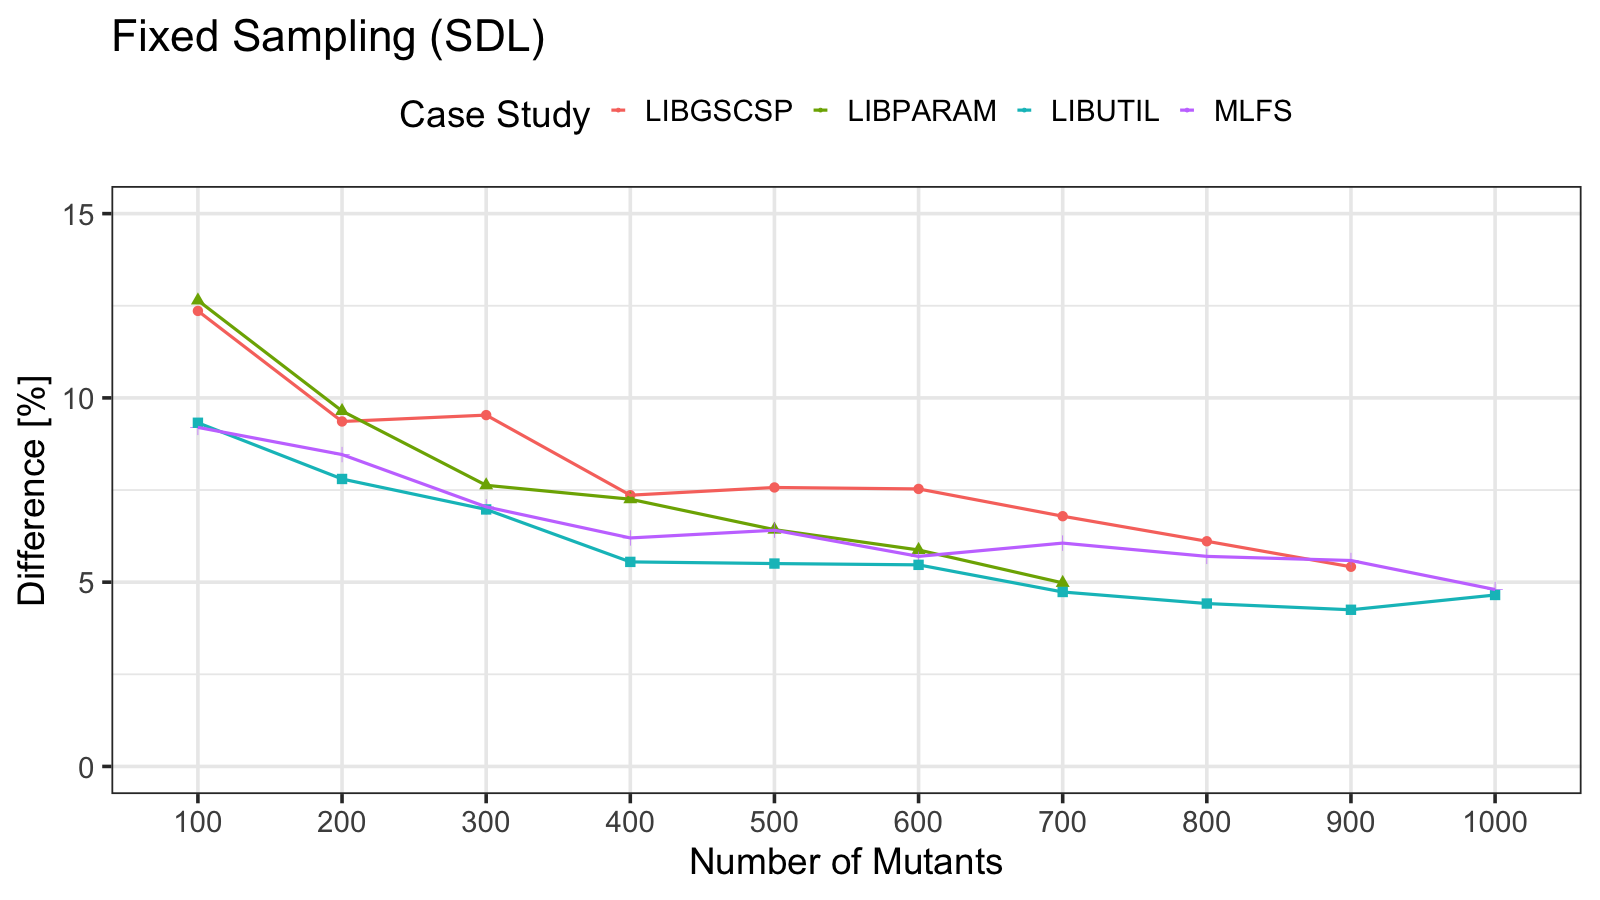
\includegraphics[width=6cm]{images/sampling_fixed_sdl}
%\caption{}
%\label{fig:results:fixedNumberOfMutantsSDL}
%\end{subfigure}
%\begin{subfigure}{.33\textwidth}
%  \centering
%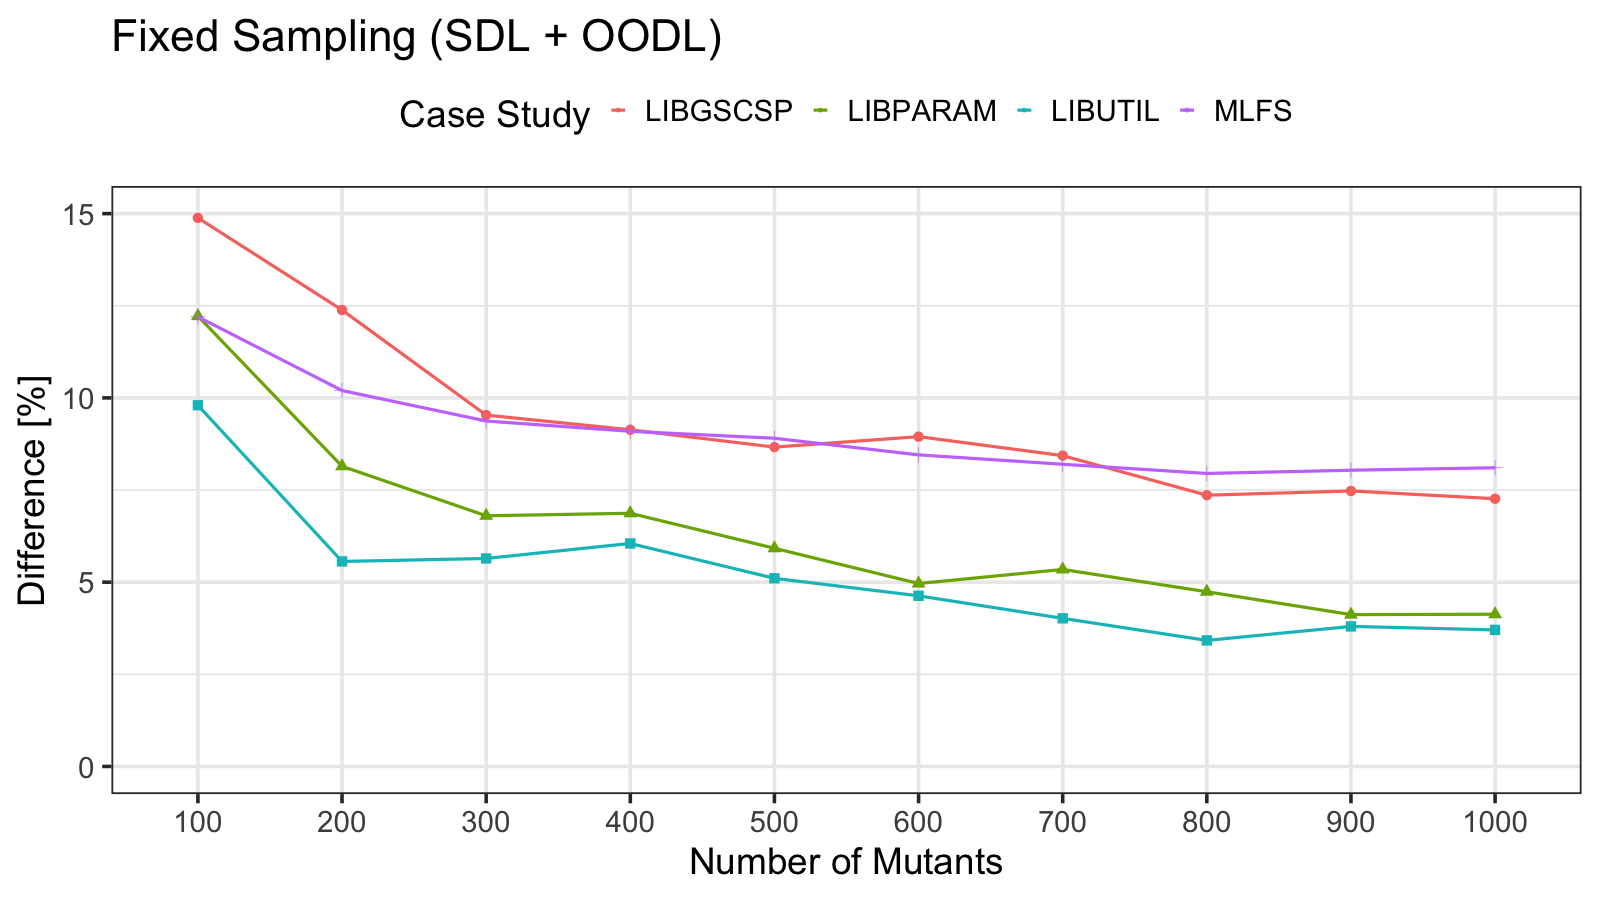
\includegraphics[width=6cm]{images/sampling_fixed_sdl_oodl}
%\caption{}
%\label{fig:results:fixedNumberOfMutantsSDLOODL}
%\end{subfigure}
%\begin{subfigure}{.33\textwidth}
%  \centering
%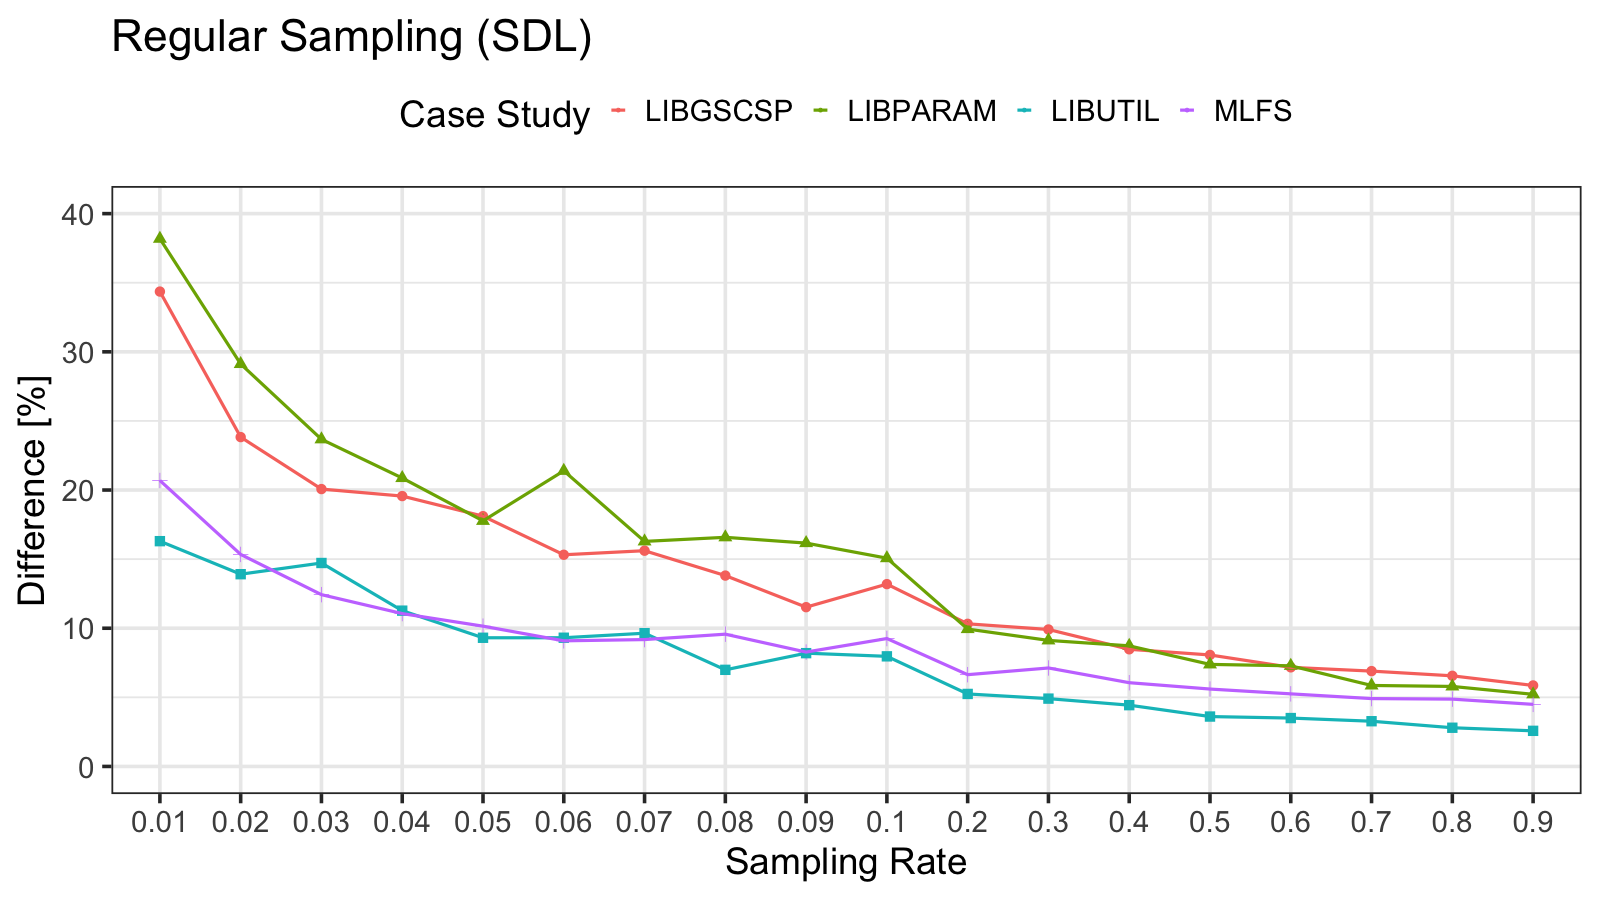
\includegraphics[width=6cm]{images/sampling_reg_sdl}
%\caption{}
%\label{fig:results:regNumberOfMutantsSDL}
%\end{subfigure}
%\begin{subfigure}{.33\textwidth}
%  \centering
%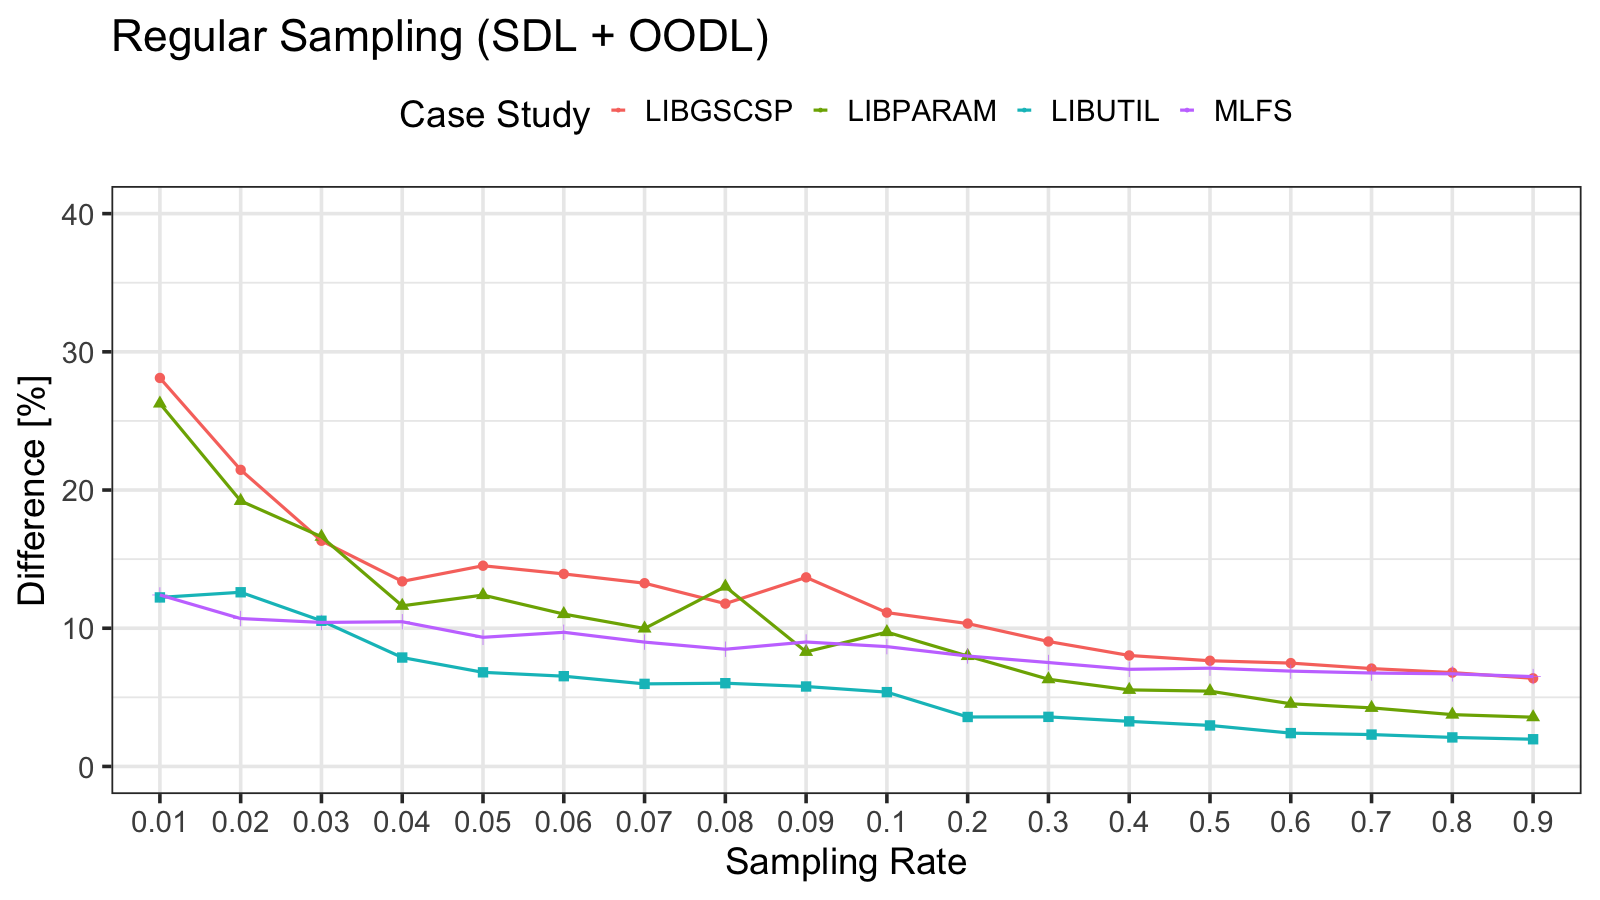
\includegraphics[width=6cm]{images/sampling_reg_sdl_oodl}
%\caption{}
%\label{fig:results:regNumberOfMutantsSDLOODL}
%
%\end{subfigure}
%\begin{subfigure}{.33\textwidth}
%  \centering
%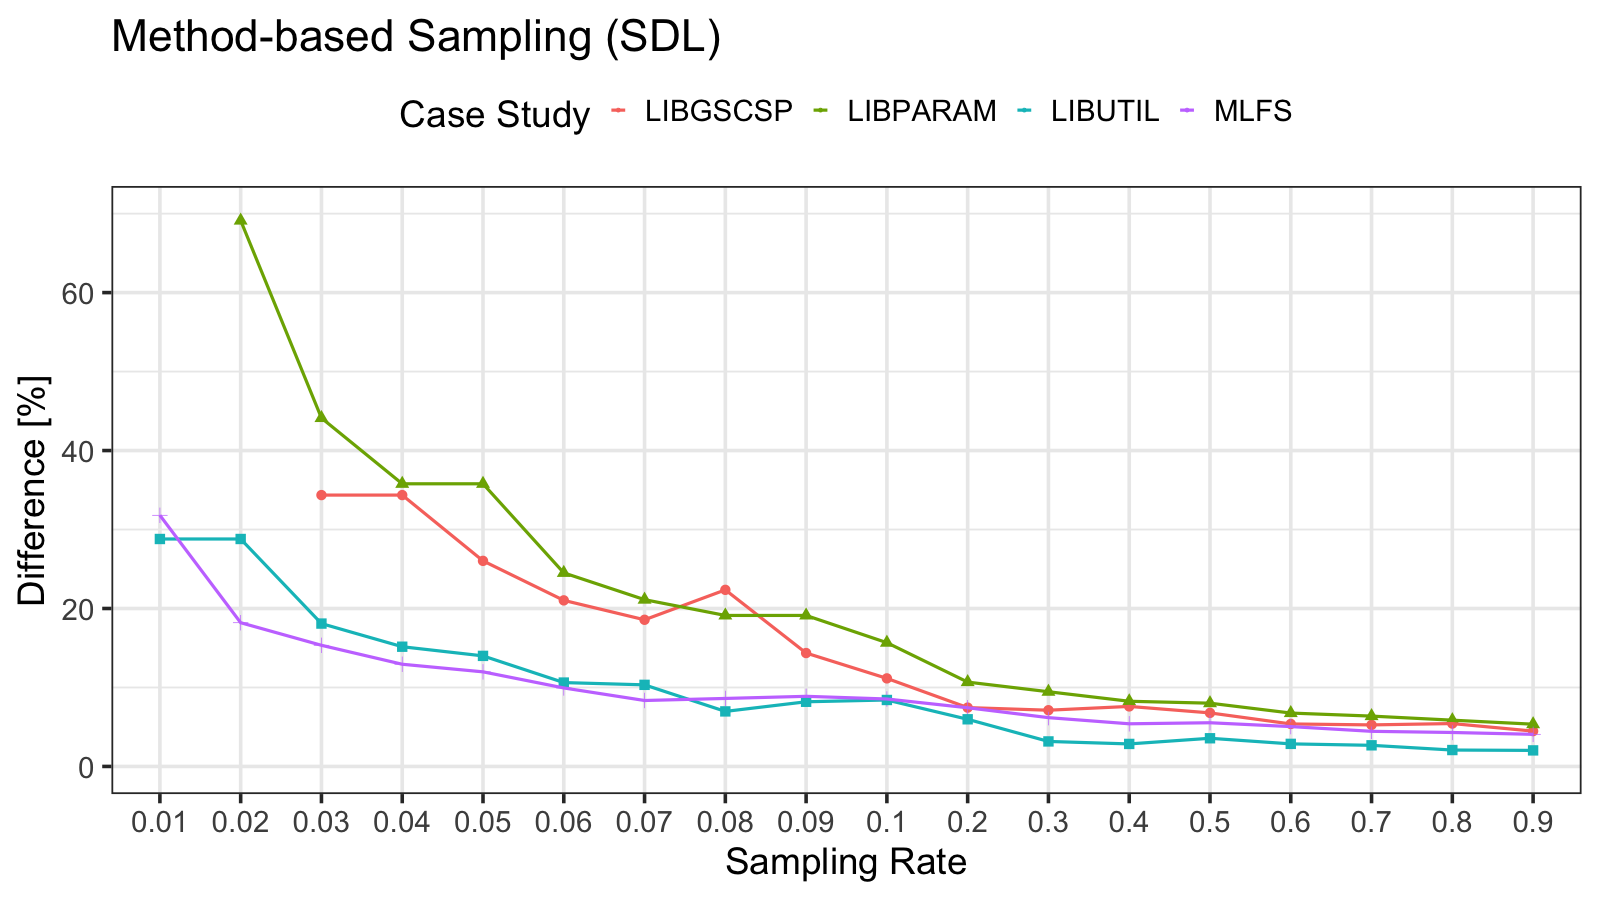
\includegraphics[width=6cm]{images/sampling_func_sdl}
%\caption{}
%\label{fig:results:funcNumberOfMutantsSDL}
%
%\end{subfigure}
%\begin{subfigure}{.33\textwidth}
%  \centering
%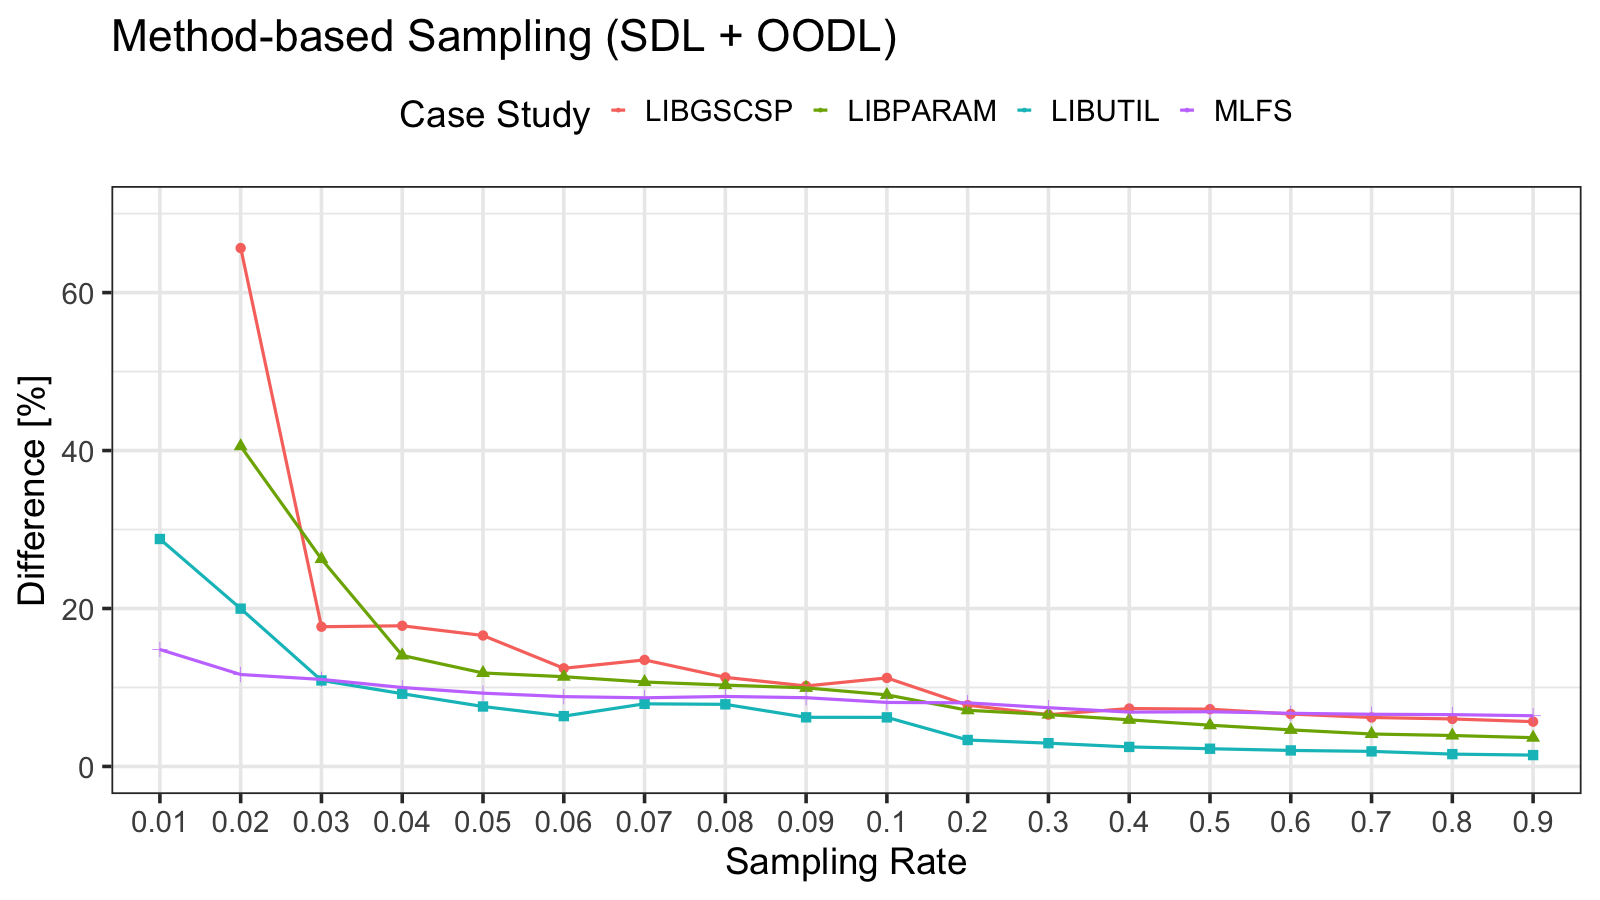
\includegraphics[width=6cm]{images/sampling_func_sdl_oodl}
%\caption{}
%\label{fig:results:funcNumberOfMutantsSDLOODL}
%
%\end{subfigure}
%\caption{}
%\label{fig:}
%\end{figure*}


\subsection{RQ4 - Mutation Score Accuracy with PrioritizeAndReduce}
\label{exp:accuracy:prioritize}

\paragraph{Design and measurements}

RQ4 assesses whether the mutation score obtained with the reduced and prioritized test suite generated by \APPR (hereafter, the \MPTS) accurately estimates the actual mutation  score.
%speeds up the mutation testing process.
To this end, we compare the accuracy obtained with the four distance metrics (i.e., $D_J$, $D_O$, $D_E$, and $D_C$) used by the proposed \INDEX{PrioritizeAndReduce} algorithm (Figure 1.6 from D2). In addition, to determine to what extent our prioritization strategy based on code coverage contributes to the selection of test cases that kill mutants, we also compare the results obtained with a simple baseline that, for each mutant, randomly selects one test case among the ones that cover the mutant. 


For all subjects, we consider (a) the complete set of mutants, (b) the reduced subset of mutants providing accurate results (i.e., the one obtained with FSCI sampling with $T_{\mathit{CI}}=0.10$). 
Based on RQ3 results, we exclude mutants generated with the SDL and SDL+OODL operators only. 
%Since, based on related work, engineers may still be interested in evaluating the mutation score obtained with SDL operators only, we study to what extent the test suite derived by the \emph{PrioritizeAndReduce} algorithm enable us to estimate the mutation score computed with the SDL operator.
For FSCI sampling, since we evaluate the accuracy of a reduced test suite, we derive the confidence interval using Equation 1.5 from D2. 
%Details about the estimated accuracy and number of mutants \ref{appendix:FSCI:reduced}.

%To the end of this research question, we study if the proposed reduction/prioritization strategies can produce a mutation score that is \textit{representative} with respect to the true mutation score obtained with no test suite reduction/prioritization strategies.

%We consider the same set of mutants as for RQ2.
For each subject and each distance metric, and for each of the two sets of mutants considered, we generated ten different \MPTSs. In the case of FSCI, since it randomly selects mutants, we considered ten different sets of mutants derived with distinct executions of the FSCI algorithm. For each \MPTS, we computed the mutation score obtained. 
Then, to determine if the mutation score of the \MPTS is accurate, we follow the same procedure adopted for RQ2, i.e., we rely on the 2.5/97.5 percentile distance from the actual mutation score. 
%In the case of the SDL set, we rely on the 2.5/97.5 percentile distance from the mutation score obtained with all the SDL mutants.



\paragraph{Results}

% !TEX root =  ../Main.tex

\begin{table}[]
\centering
\scriptsize
\caption{RQ4. Mutation score accuracy for the different strategies implemented by \emph{PrioritizeAndReduce}}
\label{table:results:PriritizeAndReduce} 
\begin{tabular}{|
p{15mm}@{\hspace{1pt}}|
p{15mm}@{\hspace{1pt}}|
>{\raggedleft\arraybackslash}p{15mm}@{\hspace{1pt}}|
>{\raggedleft\arraybackslash}p{15mm}@{\hspace{1pt}}|
>{\raggedleft\arraybackslash}p{15mm}@{\hspace{1pt}}|
}
\hline
           &          &\multicolumn{3}{c}{\textbf{$\delta_{acc}$}}\\
\hline
\textbf{Case Study} & \textbf{Strategy} & \textbf{ALL} & \textbf{FSCI (C=10)} & \textbf{SDL}  \\
\hline
\multirow{5}{*}{LIBUTIL}    
    & Random & 3.1400 & 5.87 & 3.5500  \\
           & $D_J$                    & 0.0300  & 2.54 & 0.0900  \\
           & $D_O$                    & 0.0300  & 2.54 & 0.0900  \\
           & $D_E$                    & 0.0199  & 2.51 & 0.0900  \\
           & $D_C$                    & 0.0199  & 2.57 & 0.0900 \\
\hline
\multirow{5}{*}{LIBGSCSP}   & Random & 7.2055 &  $>$5\% & 8.0605   \\
           & $D_J$                    & 1.3455  & 3.55 &1.5300 \\
           & $D_O$                    & 1.3100  & 3.55  &1.4200 \\
           & $D_E$                    & 0.7300  & 3.75  &0.6500 \\
           & $D_C$                    & 0.7300  & 3.75 &0.6500  \\
\hline
\multirow{5}{*}{LIBPARAM}   & Random & 7.7927 & $>$5\%  & 6.0892  \\
           & $D_J$                    & 0     &3.62& 0  \\
           & $D_O$                    & 0     &3.62& 0    \\
           & $D_E$                    & 0     &3.62& 0     \\
           & $D_C$                    & 0     &3.62& 0     \\
\hline
\multirow{5}{*}{MLFS}       & Random &  6.721  & $>$5\%   &    7.3999 \\
           & $D_J$                      &   0.3299   & 4.07&    0.2299    \\
           & $D_O$                      &   0.3299   & 4.07&     0.2299   \\
           & $D_E$                      &   0.0199   & 4.33&     0  \\
           & $D_C$                      &    0.0300  & 4.27&     0   \\
\hline
\multirow{5}{*}{ESAIL}      & Random & 38.8885      &   $>$5\%    &   39.1765\\
                                                & $D_J$      & 24.1688      &   $>$5\%     &  21.6800\\
                                                & $D_O$     & 24.3650      &  $>$5\%     &   21.7570\\
                                                & $D_E$     &  4.0800     &  4.7794     &   4.1400\\
                                                & $D_C$     &  3.9833    &   4.8825    &  4.5600\\
\hline
\end{tabular}
\end{table}


% \begin{table}[h]
% \centering
% \tiny
% \caption{RQ6. MS Comparison with respect to Random approach.}
% \label{table:results:msReducedRandomPVals} 
% \begin{tabular}{|llll|}
% \hline
% \textbf{Case Study}                & \textbf{\begin{tabular}[c]{@{}l@{}}MS Comparison\\w.r.t. Random\end{tabular}} & \textbf{ALL P-value} & \textbf{SDL P-value} \\
% \hline
% \multirow{4}{*}{LIBGSCSP} & $D_J$    & 1.47E-04     & 1.37E-04 \\
%                           & $D_O$    & 1.40E-04     & 1.19E-04  \\
%                           & $D_E$    & 5.18E-05     & 5.30E-05  \\
%                           & $D_C$    & 1.17E-04     & 1.08E-04  \\
% \hline
% \multirow{4}{*}{LIBUTIL}  & $D_J$    & 1.27E-04      & 1.23E-04 \\
%                           & $D_O$    & 1.20E-04      & 1.15E-04 \\
%                           & $D_E$    & 1.20E-04      & 1.15E-04  \\
%                           & $D_C$    & 1.31E-04      & 1.26E-04 \\
% \hline
% \multirow{4}{*}{LIBPARAM} & $D_J$    & 5.38E-05      & 4.96E-05 \\
%                           & $D_O$    & 5.38E-05      & 4.96E-05 \\
%                           & $D_E$    & 5.38E-05      & 4.96E-05 \\
%                           & $D_C$    & 5.38E-05      & 4.96E-05 \\
% \hline
% \multirow{4}{*}{MLFS}     & $D_J$    &  1.40E-04    &  5.30E-05\\
%                           & $D_O$    &  1.40E-04      & 5.30E-05 \\
%                           & $D_E$    &  1.36E-04      &5.30E-05 \\
%                           & $D_C$    &  1.48E-04      & 5.30E-05 \\
% \hline
% \multirow{4}{*}{ESAIL}    & $D_J$    &                \\
%                           & $D_O$    &                \\
%                           & $D_E$    &                \\
%                           & $D_C$    &               \\
% \hline
% \end{tabular}
% \end{table}



%\begin{table*}
%\tiny
%\centering
%\caption{RQ6. P-value comparison between test suite reduction approaches.}
%\label{table:results:pValComparisonTSredPrior} 
%\begin{tabular}{|l|l|lllll|l|lllll|}
%\hline
%           &          & ALL      &                       &                       &          &      &          & SDL      &                       &                       &                       &       \\
%\hline           
%Case Study &          & Random & $D_J$                  & $D_O$                  & $D_E$     & $D_C$ &          & Random & $D_J$                  & $D_O$                  & $D_E$                  & $D_C$  \\
%\hline
%LIBGSCSP   & Random &          &                       &                       &          &      & Random &          &                       &                       &                       &       \\
%           & $D_J$     & 1.47E-04 &                       &                       &          &      & $D_J$     & 1.37E-04 &                       &                       &                       &       \\
%           & $D_O$     & 1.40E-04 & 2.50E-01              &                       &          &      & $D_O$     & 1.18E-04 & 7.88E-02              &                       &                       &       \\
%           & $D_E$     & 5.18E-05 & 5.15E-05              & 4.81E-05              &          &      & $D_E$     & 5.30E-04 & 4.56E-04              & 3.80E-05              &                       &       \\
%           & $D_C$     & 1.17E-04 & 1.16E-04              & 1.10E-04              & 2.93E-02 &      & $D_C$     & 1.08E-04 & 9.55E-05              & 8.21E-05              & 6.71E-02              &       \\
%\hline
%LIBUTIL    & Random &          &                       &                       &          &      & Random &          &                       &                       &                       &       \\
%           & $D_J$     & 1.27E-04 &                       &                       &          &      & $D_J$     & 1.23E-04 &                       &                       &                       &       \\
%           & $D_O$     & 1.20E-04 & 8.31E-01              &                       &          &      & $D_O$     & 1.15E-04 & 8.31E-01              &                       &                       &       \\
%           & $D_E$     & 1.20E-04 & 8.38E-03              & 2.05E-03              &          &      & $D_E$     & 1.15E-04 & 8.31E-01              & \multicolumn{1}{r}{1} &                       &       \\
%           & $D_C$     & 1.31E-04 & 6.40E-03              & 2.20E-03              & 5.34E-01 &      & $D_C$     & 1.26E-04 & 6.80E-01              & 5.34E-01              & 5.34E-01              &       \\
%\hline
%LIBPARAM   & Random &          &                       &                       &          &      & Random &          &                       &                       &                       &       \\
%           & $D_J$     & 5.38E-05 &                       &                       &          &      & $D_J$     & 4.96E-05 &                       &                       &                       &       \\
%           & $D_O$     & 5.38E-05 & \multicolumn{1}{r}{1} &                       &          &      & $D_O$     & 4.96E-05 & \multicolumn{1}{r}{1} &                       &                       &       \\
%           & $D_E$     & 5.38E-05 & \multicolumn{1}{r}{1} & \multicolumn{1}{r}{1} &          &      & $D_E$     & 4.96E-05 & \multicolumn{1}{r}{1} & \multicolumn{1}{r}{1} &                       &       \\
%           & $D_C$     & 5.38E-05 & \multicolumn{1}{r}{1} & \multicolumn{1}{r}{1} &    \multicolumn{1}{r}{1}   &      & $D_C$     & 4.96E-05 & \multicolumn{1}{r}{1} & \multicolumn{1}{r}{1} & \multicolumn{1}{r}{1} &       \\
%\hline
%MLFS       & Random &          &                       &                       &          &      & Random &          &                       &                       &                       &       \\
%           & $D_J$     & 1.40E-04 &                       &                       &          &      & $D_J$     & 5.30E-05 &                       &                       &                       &       \\
%           & $D_O$     & 1.40E-04 & \multicolumn{1}{r}{1} &                       &          &      & $D_O$     & 5.30E-05 & \multicolumn{1}{r}{1} &                       &                       &       \\
%           & $D_E$     & 1.36E-04 & 1.20E-04              & 1.20E-04              &          &      & $D_E$     & 5.30E-05 & 1.31E-05              & 1.31E-05              &                       &       \\
%           & $D_C$     & 1.48E-04 & 1.31E-04              & 1.31E-04              & 1.61E-02 &      & $D_C$     & 5.30E-05 & 1.31E-05              & 1.31E-05              & \multicolumn{1}{r}{1} &       \\
%\hline
%ESAIL      & Random &          &                       &                       &          &      & Random &          &                       &                       &                       &       \\
%           & $D_J$     &          &                       &                       &          &      & $D_J$     &          &                       &                       &                       &       \\
%           & $D_O$     &          &                       &                       &          &      & $D_O$     &          &                       &                       &                       &       \\
%           & $D_E$     &          &                       &                       &          &      & $D_E$     &          &                       &                       &                       &       \\
%           & $D_C$     &          &                       &                       &          &      & $D_C$     &          &                       &                       &                       &      \\
%\hline           
%\end{tabular}
%\end{table*}




Table~\ref{table:results:PriritizeAndReduce} provides the values of $\delta_{acc}$ obtained for the different subjects and distance metrics (i.e., the random baseline and the four distance metrics supported by \APPR). Rows named \emph{ALL} report the results obtained when executing the entire set of mutants, rows named \emph{FSCI}  report the results obtained  with the FSCI strategy. 
%column \emph{SDL} reports the results for the mutants generated with the SDL operator only.



\NEWFSCI{Unsurprisingly, for all the subjects except \SAIL{}$_S$, the mutation score computed with the entire set of mutants tested with the \MPTS (i.e., row ALL) is more accurate than the mutation score computed with a subset of the mutants tested with the same test suite (i.e., row FSCI). 
%However, the distance metrics $D_E$ and $D_C$ enable the accurate estimation (i.e, $\delta_{acc}  < 5$) of the actual mutation score with FSCI.
However, the mutation score estimated with FSCI is always accurate (i.e, $\delta_{acc}  < 5$).
In the case of \SAIL{}$_S$, where each statement is covered by a large number of test cases (see Section~\ref{sec:empirical:subjects}),
%\footnote{\UPDATE{In $ESAIL_S$, each statement is covered on average by 61 test cases. In the other cases, each statement is covered by 2 test cases, on average (see Section~\ref{sec:empirical:subjects}).}}, 
test suite reduction has a higher probability of retaining a test case that does not kill a mutant.
For this reason, executing a reduced test suite with a subset of mutants selected with FSCI, which estimates the error due to test suite reduction, 
leads to a more accurate mutation score than executing a reduced test suite with the entire set of mutants without estimating such error (i.e., row ALL).
%For this reason, FSCI, which estimates the error due to test suite reduction, 
%performs better.
% than the execution of the entire set of mutants without estimating such error (i.e., row ALL).
%FSCI enables a more accurate computation of the mutation score for the \MPTS. 
%\FIXME{It happens because estimation errors due to test suite reduction are minimal
%\footnote{Figure~\ref{} shows that the number of test cases executed by FSCI with the whole test suite is similar to the one with the reduced test suite}, consequently 
%enforcing $|\mathit{CI}_E| \le T_{\mathit{CE}}$ simply augment the sample size thus improving the accuracy of the estimation.}
}

%enforcing PKErr, which is used to compute a corrected confidence interval and consequently the mutation score. The corrected confidence interval, which takes into account PKErr enable us to obtain a more accurate mutation score than the one computed with the whole test suite. Which is an additional reason for adopting FSCI.}}
 

%% Comment 25/02/2021:
%% In the case of ESAIL, the higher delta is likely due to the large number of test cases covering each mutant, which increases the likelihood of removing  test cases that kill the mutant. Consequently, the mutation score may be affected. In the case of FSCI, such error in the computation score is estimated with the initial tuning to estimate PKErr, which is used to compute a corrected confidence interval and consequently the mutation score. The corrected confidence interval, which takes into account PKErr enable us to obtain a more accurate mutation score than the one computed with the whole test suite. Which is an additional reason for adopting FSCI.
%% For reviewer: we realized with additional experiments, that the updated procedure lead to a mutation score that is more accurate than the mutation score computed with the whole set of mutants.


The only distance metric that consistently leads to inaccurate estimates of the mutation score (i.e., $\delta_{acc}  > 5$) across subjects is the random baseline.
Based on a non-parametric Mann Whitney test, the difference between the random baseline (i.e., Random) and the four distance metrics implemented by \APPR (i.e., $D_*$) is always significant with a \textit{p}-value $< 0.05$. This indicates that \textbf{the \APPR distance metrics are necessary to accurately estimate the mutation score while reducing the number of test cases to  execute}.

Among the proposed distance metrics, 
$D_J$ and $D_O$ provide inaccurate results with \SAIL{}$_S$.
%and less accurate results for other subjects than alternatives. 
We conjecture the main reason is their inability to account for the number of times a statement is exercised by a test case. 
We believe this is an important factor as system test cases that repeatedly exercise mutated statements, with different variable values, are more likely to kill mutants than test cases exercising such statements only once (e.g., because of the uncertainty regarding the 
\JMR{3.16}{incorrect intermediate state
%infected program state
propagating to the state variables verified by test oracles, see Section~1.2.1.1 from D2}). On the other hand, unit and integration test cases, which exercise much simpler scenarios in other subjects, are more likely to kill a mutant when the mutated statement is executed only once (e.g., because the oracle is closer to the mutated statement). This is why $D_J$ and $D_O$ fare similarly to the other distance metrics for these subjects. 
%Almost every system test case exercises certain components (e.g., the handler of telecommands, which is the main entry point of the system) but only the ones executing such components repeatedly (e.g., to verify multiple combination of input values for a same telecommand) carefully exercise mutated statements. Regarding the other subjects, each unit and integration test case rather tends to focus on simple test scenarios that exercise mutated statements once or a few times.
In contrast, $D_C$ and $D_E$ are distance metrics ensuring an accurate estimate of the mutation score and providing the lowest $\delta_{acc}$. The differences between $D_E$ and $D_C$ are always statistically significant, \UPDATE{except for \MLFS{}{}}. However, there are no practically significant differences between them. 
Since $D_C$ provides a normalized score, which is required by Step 8, we select $D_C$ as the preferred metric to be used in \APPR.
%the Based on $\delta_{acc}$, the metric that perform slightly better is $D_E$ (the sum of the $\delta_{acc}$ across all the case studies for all the configurations is lower than for $D_E$. \textbf{We thus select $D_E$ as the best metric to be used with \APPR}.


\subsection{RQ5 - Time Savings with PrioritizeAndReduce}

\paragraph{Design and measurements}

RQ5 assesses to what extent  the \MPTS speeds up the mutation analysis process.


For each subject considered for RQ4, we measure the execution time taken by the \MPTS to execute on the mutants.
We compute time saving as the ratio of the difference in execution time from the original test suite over the time it requires to execute, for the set of mutants selected.
In particular, as in RQ4, we consider three scenarios (1) all the mutants are selected, (2) mutants are selected with FSCI sampling, (3) mutants are selected with FSCI sampling but we execute the entire test suite, as opposed to the \MPTS. By considering scenario (3), we can estimate both the time saved thanks to mutant sampling and the additional time saved when combining it with the \MPTS.
For the original test suite, to emulate a realistic mutation analysis process according to state-of-the-art solutions, we measure the time required to execute test cases until the mutant is killed (for live mutants it means that we execute the entire test suite). Also, we set a test case timeout equal to three times the duration of the original test case.

Since the execution time of test cases depends on multiple factors such as the underlying test harness, the development practices in place (e.g., verifying multiple scenarios in a single test case), and the type of testing conducted (e.g., unit, integration, system), we also compute 
the ratio of the number of test cases not executed by the \MPTS over the total number of test cases.

\paragraph{Results}

Table~\ref{table:time:original} reports, for every subject, the time required to test all the mutants with the entire test suite, in seconds. It also reports  the total number of test cases executed. 
We observe that mutation analysis requires a large amount of time. It takes between 13 and 73 hours for subjects tested with unit and integration test suites (which are faster to execute). When a system test suite needs to be executed (i.e., $\mathit{\SAIL{}_S}$), traditional mutation analysis becomes infeasible as shown by the 11,000 hours required to perform mutation analysis with $\mathit{\SAIL{}_S}$.

Figures~\ref{fig:results:time:saving} and~\ref{fig:results:test:saving} provide boxplots depicting 
the saving achieved when the \MPTS is executed with all the mutants and with the FSCI-selected mutants, in terms of execution time and test cases, respectively. Each observation corresponds to the saving obtained with one of the ten executions performed on each subject, for a specific configuration (i.e., distance $D_*$ and strategy adopted for selecting mutants). In Figures~\ref{fig:results:time:saving} and~\ref{fig:results:test:saving}, horizontal dashed lines show the average across all subjects, whiskers are used to identify outliers (i.e., they are placed below/above 1.5*Inter Quartile Range of the upper quartile/lower quartile). A detailed table including min, max, mean, and median values for each subject is provided in Appendix C.
%~\ref{appendix:details:rq5}.

%Table~\ref{table:results:reduction:prioritize} reports the saving achieved when the \APPR test suite is executed with all the mutants, with the FSCI selected mutants, with the SDL mutants. For both time savings and test savings, we report the min, max, median, and mean values. Values are reported for all the case studies, for all the distance metrics, and for the three strategies considered to select mutants (i.e., selecting all the available mutants, selecting all the mutants generated with the SDL operator, and selecting mutants with the FSCI strategy).

Unsurprisingly, the smallest reduction in execution time and number of executed test cases is achieved when executing the \MPTS with all the mutants. 
Measuring such time reduction allows us to evaluate the benefits of test suite prioritization and selection when it is not combined with mutant selection.
Excluding outliers, execution time reduction goes from  \UPDATE{-0.52\%} % -0.11\% was the 1st quantile not the whisker
to 16.82\% and appears to be correlated with the reduction in number of test cases to execute, which varies from 4.80\% to 33.17\%.
The largest reductions are obtained with $D_J$ and $D_O$ (the median is 13.36 and 13.40, respectively), which do not consider differences in coverage frequency, thus removing the largest number of test cases; however, $D_J$ and $D_O$ also lead to the worst accuracy results according to RQ4. Metrics $D_C$ and $D_E$, instead, lead to limited benefits in terms of time reduction.

A negative reduction indicates that the reduced and prioritized test suite increases the execution time of the mutation analysis process. This happens when (1) test cases are sorted in such a way that test cases that kill the mutants are executed later with respect to the original test suite, (2) test cases that kill the mutants but have long execution times (e.g., because they trigger a timeout) are executed before test cases with shorter execution times that kill the mutants. Negative reduction, however, affects only a few executions, thus showing that a reduced and prioritized test suite tends overall to be beneficial to the mutation analysis process.



%With our subject artifacts, in terms of execution time, test suite prioritization is thus not always beneficial; however, it always lead to a reduction the number of test cases between 4.82 and 33.15. The distance metrics leading to the highest reduction in the number of test cases are $D_J$ and $D_O$, i.e., the ones with the lowest accuracy computed for RQ 4.

Mutant sampling alone contributes to a high reduction in execution time; indeed, in Figure~\ref{fig:results:time:saving}, the boxplot \emph{FSCI 0.1-Full TS}, depicting the time saving for FSCI mutants tested with the entire test suite, shows minimum, median, and maximum values of 65.76\%, 75.10\%, and 84.72\%. Indeed, by reducing the number of mutants to execute, FSCI sampling significantly reduced the total number of test cases to execute within a [\JMRCHANGE{49.98\%} - 80.54\%] range (as shown by the boxplot in Figure~\ref{fig:results:test:saving}).

The highest reduction in execution time is achieved when combining the \MPTS with FSCI sampling. It ranges from 72.09\% to 90.83\%. $D_C$ and $D_E$, which are the approaches that guarantee accurate results, lead to an execution time reduction in the ranges \JMRCHANGE{[75.25\% - 90.83\%]} and \JMRCHANGE{[73.53\% - 90.83\%]}, respectively, an impressive achievement. 
Test case savings, 
%show similar ranges, 
\JMRCHANGE{as well, are above 65\%, [68.28\% - 83.45\%]} and \JMRCHANGE{[68.08\% - 82.70\%]} for $D_C$ and $D_E$, respectively. Based on savings results, there is no practical difference between $D_C$ and $D_E$.

%The number of test cases being executed is reduced by 84.50\% for $D_J$ and $D_O$ and by 84.08\% for $D_E$ and $D_C$. When combined with FSCI sampling the differences between the different distance metrics are thus not practically significant (27 minutes, in total, across all the case studies), the selection of the coverage distance metric $D_*$ can thus rely on RQ4 results.

To conclude, \textbf{we suggest to combine FSCI sampling with the \MPTS to minimize the time required by mutation analysis}. 
For $\mathit{\SAIL{}}_S$, 
\NEWFSCI{on average, when combining the \MPTS with FSCI sampling, mutation analysis time goes from 11,000 hours to 1,531 hours, which makes mutation analysis feasible in one week with 10 computing nodes.} Note that for safety or mission critical systems, such as satellites software, the cost of using computing nodes is minimal compared to the development cost of the entire system. Indeed, to test such systems, even paying for the computational power of 100 HPC nodes to make mutation analysis feasible in half a day, is economically justifiable. \JMR{2.2}{Otherwise, without \APPR, mutation analysis leads to 11,000 hours of test cases execution, thus being practically infeasible since it would require more than 100 days to be completed, even with 100 HPC nodes.}

Our results also show that when it is not feasible to collect coverage data for the mutants under test (a requirement to generate the \MPTS), \textbf{FSCI sampling alone, without a reduced test suite, may still provide a high reduction in execution time}. In the case of $\mathit{\SAIL{}}_S$, this leads to 2,920 mutation analysis hours, which require less than two days with 100 HPC nodes.

% !TEX root =  ../Main.tex

\begin{table}[tb]
\caption{Execution time and number of test cases executed when mutation testing is based on the original test suite.}
\label{table:time:original} 
\scriptsize
\begin{tabular}{|
p{12mm}@{\hspace{2pt}}|
>{\raggedleft\arraybackslash}p{44mm}@{\hspace{1pt}}|
>{\raggedleft\arraybackslash}p{12mm}@{\hspace{1pt}}|
}
\hline
\textbf{Component}&\multicolumn{1}{c|}{\textbf{Execution time}}&\multicolumn{1}{c|}{\textbf{\# Test cases}}\\
\hline
\multirow{1}{*}{ESAIL$_S$}& 39\,604\,457 seconds (~ 11\,000 hours) & 155\,751 \\
%& SDL& & \\
\hline
\multirow{1}{*}{LIBGSCSP}&  252776 seconds (~70 hours)& 10250\\
%& SDL& 53074& 2103\\
\hline
\multirow{1}{*}{LIBPARAM}&  47949 seconds (~13 hours)& 6629\\
%& SDL& 7321& 1269\\
\hline
\multirow{1}{*}{LIBUTIL}&  214016 seconds (~59 hours)& 17672\\
%& SDL& 37603& 3030\\
\hline
\multirow{1}{*}{MLFS}&  171790 seconds (~48 hours)& 28159\\
%& SDL& 13492& 2220\\
%MLFS$_V$& 31526 &T &28069&89.03\% &X\\
\hline
\textbf{Total}&   & \\ 
\hline
\end{tabular}
\end{table}

\begin{figure}[tb]
\begin{center}
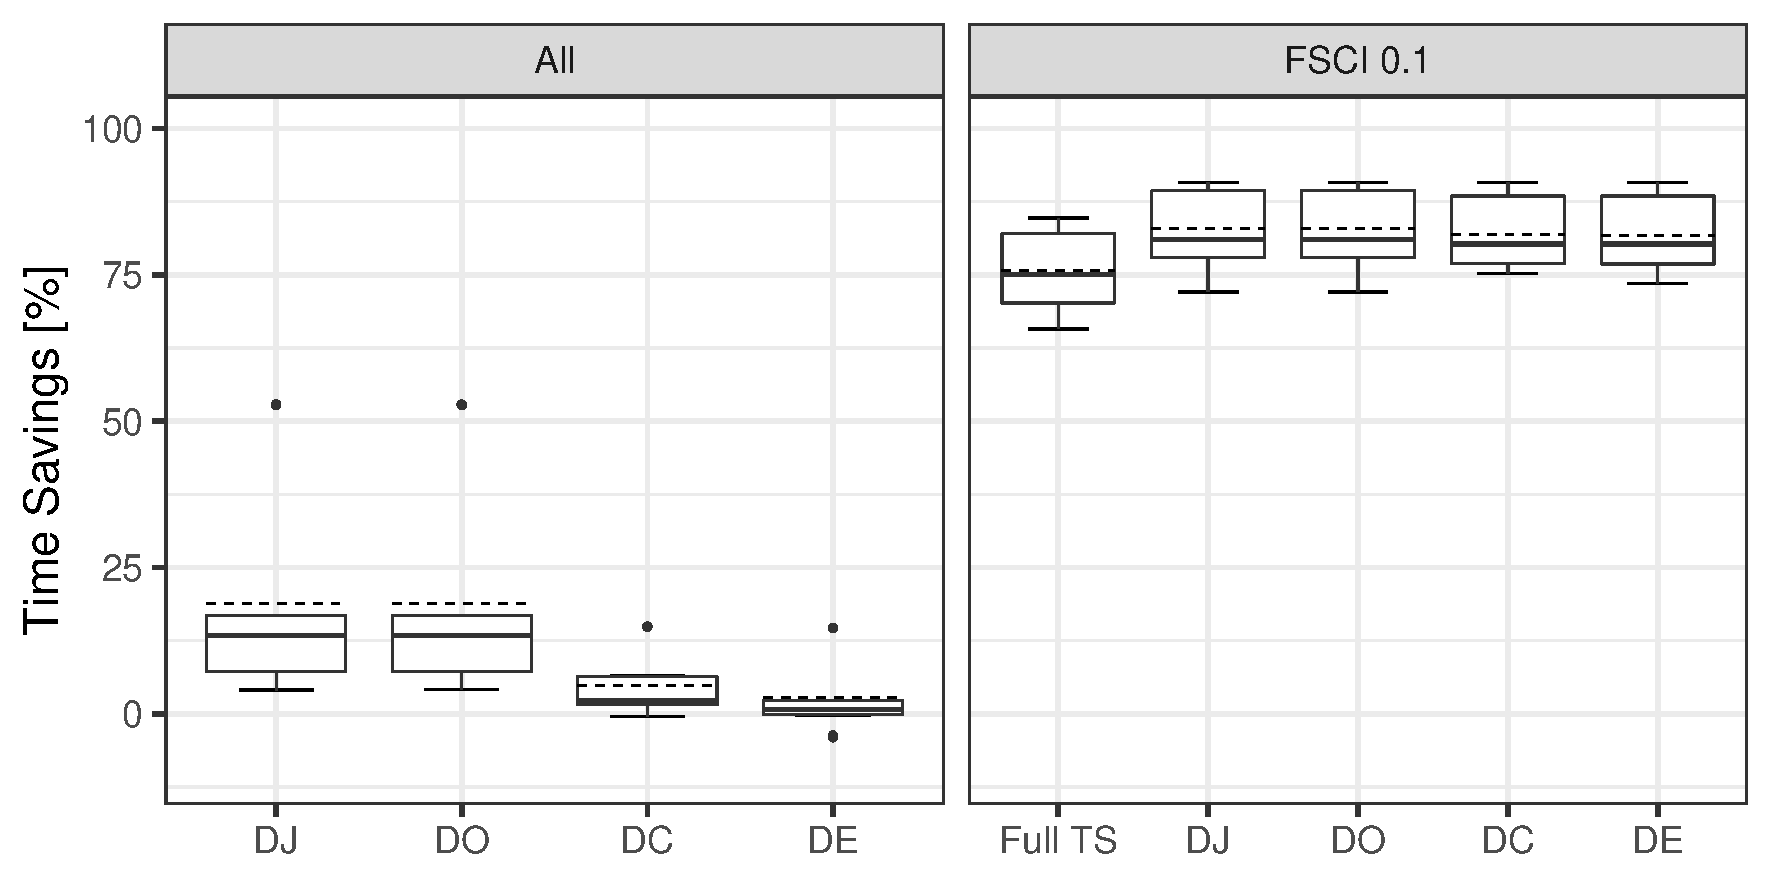
\includegraphics[width=0.8\columnwidth]{images/times.pdf}
\caption{Time savings for different sets of mutants, with the \MPTS being generated based on different distance measures.}
\label{fig:results:time:saving}
\end{center}
\end{figure}

\begin{figure}[tb]
\begin{center}
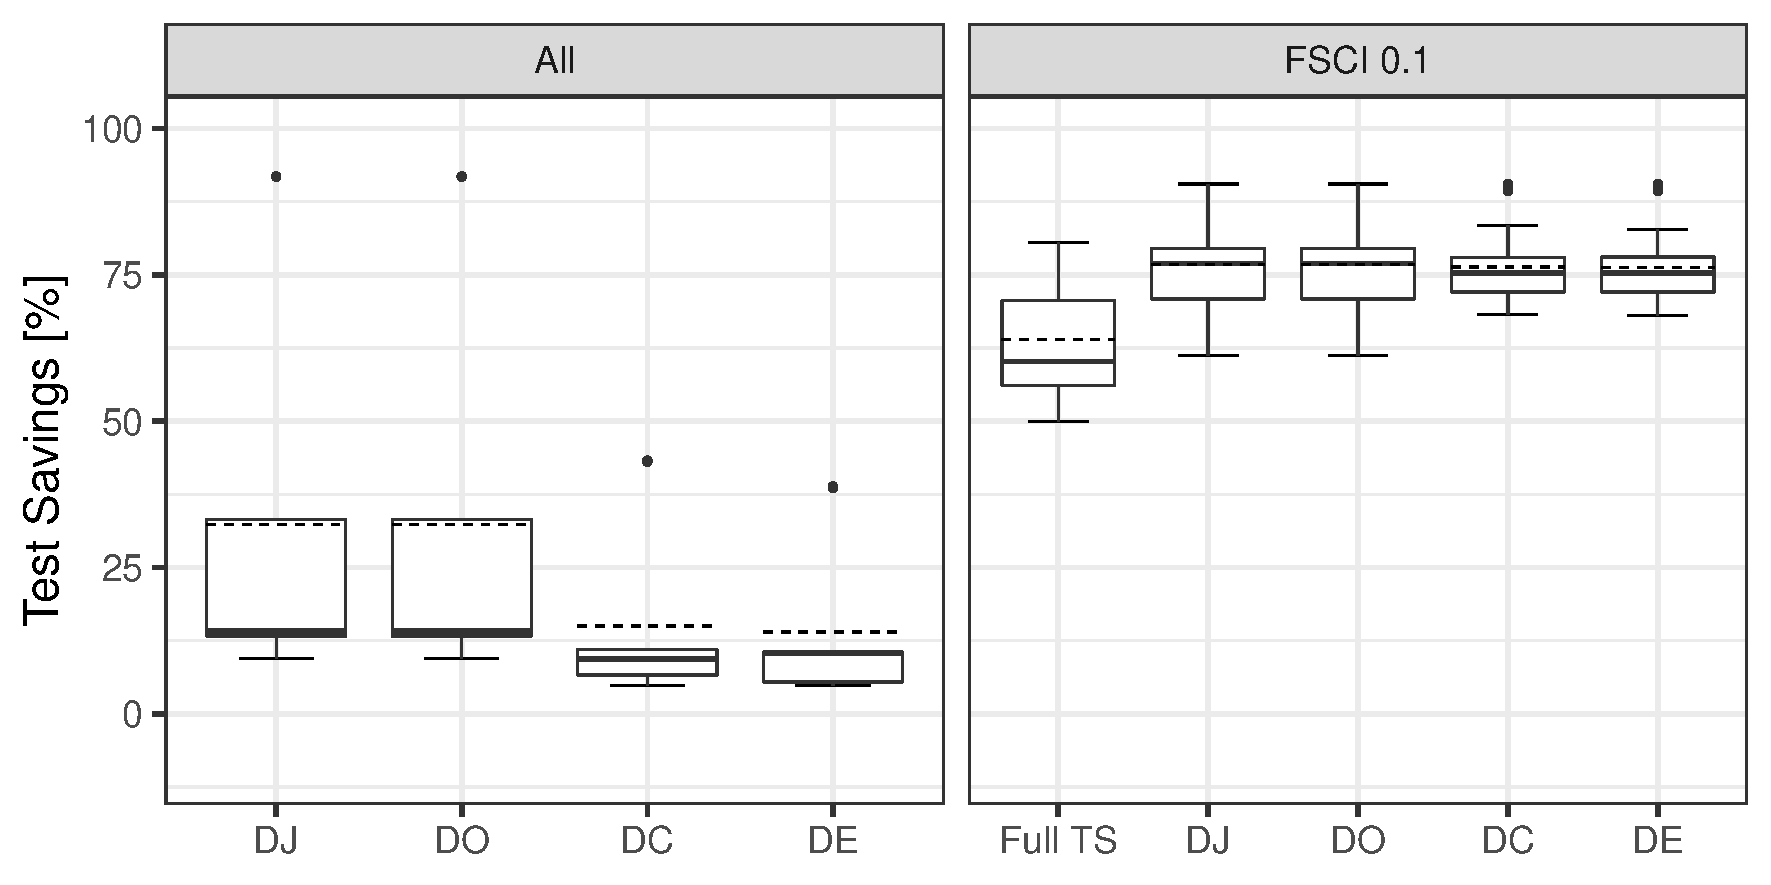
\includegraphics[width=0.8\columnwidth]{images/tests.pdf}
\caption{Test case savings for different sets of mutants, with the \MPTS being generated based on different distance measures.}
\label{fig:results:test:saving}
\end{center}
\end{figure}




\subsection{RQ6 - Precise Detection of Equivalent and Duplicate Mutants}
\label{sec:empirical:thrshold}
\paragraph{Design and measurements}
RQ6 investigates if it is possible to identify thresholds that enable the accurate identification of mutants that are nonequivalent ($T_E$) and nonduplicate ($T_D$), following the procedure described in Section 1.2.3.7 from D2.

To determine $T_E$ and $T_D$, 
we rely on the optimal distance metric identified in RQ4 ($D_C$).
%for each normalized distance metric ($D_J$, $D_O$, $D_E$, $D_C$), 
We analyze  precision and recall of the results obtained for  different values of $T_E$ and $T_D$.
%being equal to $0.0$, between $0.0$ and $0.4$,  between $0.4$ and $0.8$, between $0.8$ and $1$.
%\CHANGED{We do not discuss recall (i.e., the percentage of equivalent mutants detected by our approach) since it is not feasible to compute the overall number of equivalent, live mutants. Indeed, it would imply manually inspecting all the live mutants, 12,330 in total, across all subjects (see Table~\ref{table:results:accuracy:full}).}
%being equal to $0.0$, $0.4$, and $0.8$.
To determine $T_E$, we measure
precision as the percentage of mutants with a distance above $T_E$ that are nonequivalent, recall as the percentage of nonequivalent mutants with a distance above $T_E$.
To determine $T_D$, we measure
precision as the percentage of mutant pairs with a distance above $T_D$ that are duplicate, recall as the percentage of duplicate mutant pairs that have a distance above $T_D$.
%\CHANGED{We do not discuss recall (i.e., the percentage of equivalent mutants detected by our approach) since it is not feasible to compute the overall number of equivalent, live mutants. Indeed, it would imply manually inspecting all the live mutants, 12,330 in total, across all subjects (see Table~\ref{table:results:accuracy:full}).}

Since the quality of results might be affected by both test suite reduction (i.e., less coverage data may be available) and mutants sampling (e.g., less mutants might be sampled), consistent with the finding of previous RQs, we consider the following two configurations: 
\begin{itemize}
\item Execution of the original test suite with all the generated mutants (ALL)
%\item Execution of the original test suite against a random selection of x\% mutants
%\item Execution of the original test suite against a random selection of x\% SDL mutants
%the following might become model-based
%\item Execution of the \APPR test suite with a random selection of x\% mutants
\item Execution of the \MPTS with FSCI sampling (\APPR)
\end{itemize}

\begin{figure}[tb]
\begin{center}
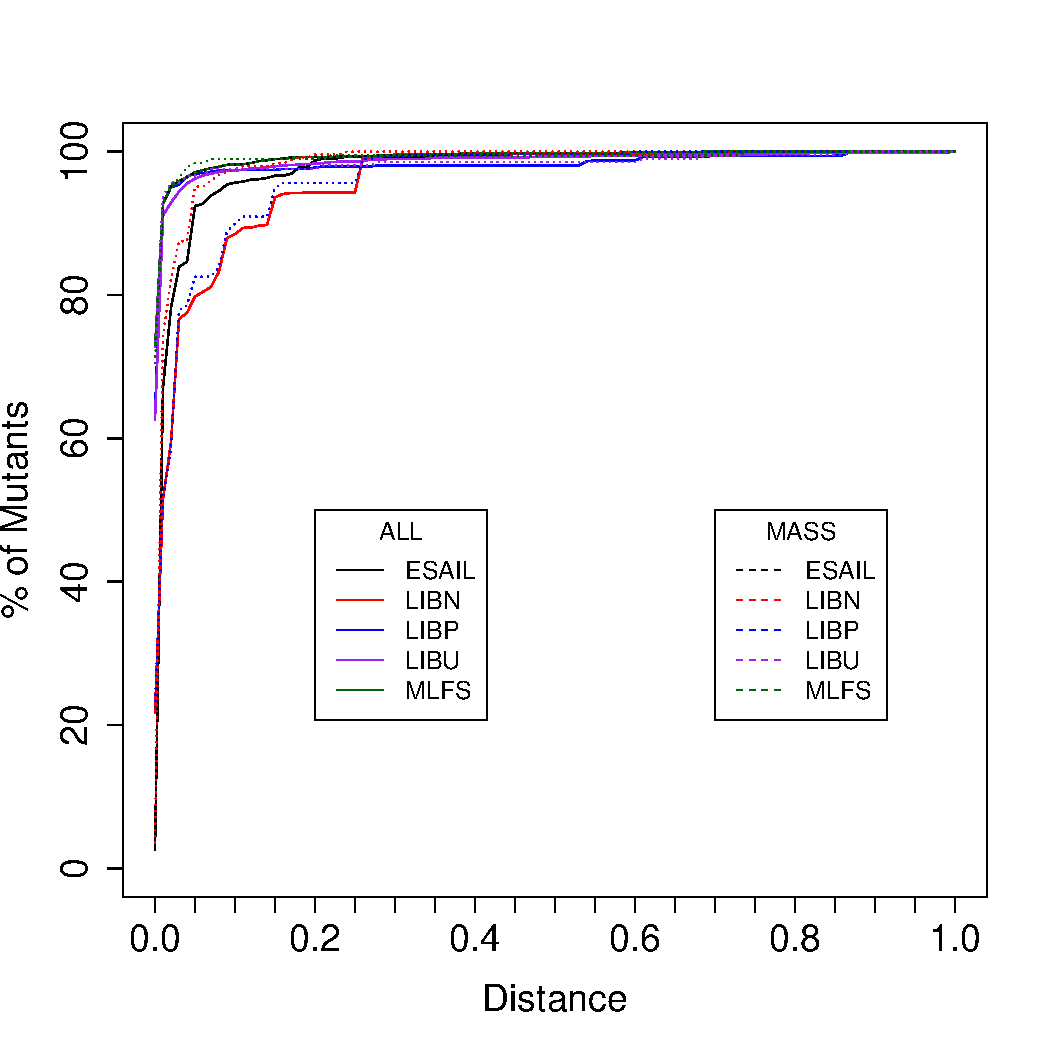
\includegraphics[width=0.6\columnwidth]{data/distanceFequency_Equivalent.pdf}
\caption{Cumulative distribution of mutants over distance values computed to determine equivalent mutants.}
\label{fig:results:test:dde}
\end{center}
\end{figure}

\begin{figure}[tb]
\begin{center}
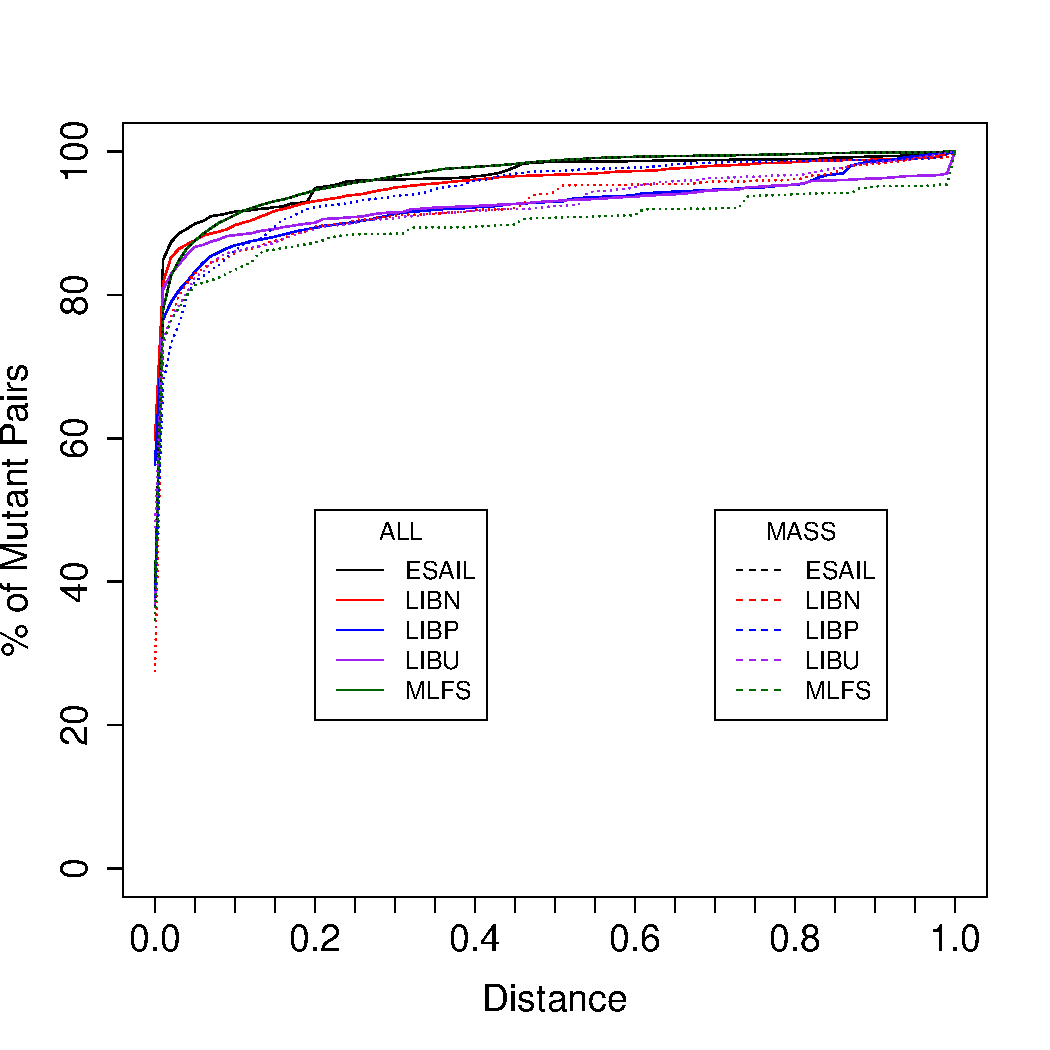
\includegraphics[width=0.6\columnwidth]{data/distanceFequency_Redundant.pdf}
\caption{Cumulative distribution of mutant pairs over distance values computed to determine duplicate mutants.}
\label{fig:results:test:ddd}
\end{center}
\end{figure}



We determine the values of $T_E$ and $T_D$ based on the analysis of the 
cumulative distribution of the distance values computed to determine equivalent and duplicate mutants, for the two configurations listed above.
Figures~\ref{fig:results:test:dde} and
~\ref{fig:results:test:ddd}
show the cumulative distribution --- the Y-axis shows the percentage of mutants and mutant pairs with a distance lower or equal to the value in the X-axis.
For both Figures~\ref{fig:results:test:dde} and
~\ref{fig:results:test:ddd} we can observe that the distribution of mutants is not uniform in the range 0-1 (otherwise we would have straight lines with 45 degree angle) but we observe a large proportion of mutants (Figures~\ref{fig:results:test:dde}) and mutant pairs (Figures~\ref{fig:results:test:ddd}) having small distances. For example,
Figure~\ref{fig:results:test:dde} shows that, across all subjects, more than 60\% of the mutants have a distance below 0.05 (i.e., with $x$ equal to $0.05$, the value of $y$ is above $60$). 
%Also, for \PARAM{}, \UTIL{}, and \MLFS{}{} more than half of the mutants have a distance equal to zero (i.e., all the test cases show the same coverage of the original program). 
%This observation, i.e., a large percentage of mutants with a small distance from the original program, should be expected since mutation operators introduce small changes into the source code which unlikely lead to big changes to the program behaviour.
%Figure~\ref{fig:results:test:ddd} shows a similar distribution for the distances computed for duplicate mutants.

To evaluate precision and recall, we thus select values for $T_D$ and $T_E$ that 
either largely differ (i.e., $0.0$, $0.4$, and $0.8$) or delimit ranges including a large proportion of the mutants (i.e., $0$, $0.01$, and $0.05$). Table~\ref{table:results:proportion:mutants} reports the percentage of mutants and mutant pairs belonging to the ranges delimited by the selected values, for the two configurations considered in our study; the distribution of mutants in Table~\ref{table:results:proportion:mutants} is consistent with Figures~\ref{fig:results:test:dde} and
~\ref{fig:results:test:ddd}.

% !TEX root =  ../Main.tex

% \begin{table}[h]
% \caption{RQ7. Precision of Coverage-Based Detection of Equivalent Mutants.}
% \label{table:results:precision:equivalent} 
% \tiny
% \begin{tabular}{|
% p{10mm}|p{10mm}|p{10mm}|
% p{3mm}|p{3mm}|p{3mm}|p{3mm}|p{3mm}|p{3mm}|p{3mm}|p{3mm}|p{3mm}|p{3mm}|
% p{3mm}|p{3mm}|p{3mm}|p{3mm}|p{3mm}|p{3mm}|p{3mm}|p{3mm}|p{3mm}|p{3mm}|
% |}
% \hline
% \textbf{Case Study}&\textbf{Operators}&\textbf{Sampling}&\multicolumn{9}{c|}{\textbf{Precision of equivalent mutants detection when distance $< T_E$.}}&\multicolumn{9}{c|}{\textbf{Precision of redundant mutants detection when distance $< T_R$.}}\\ 
% &&
% &\textbf{0.0}&\textbf{0.0}&\textbf{0.30}&\textbf{0.40}&\textbf{0.50}&\textbf{0.60}&\textbf{0.70}&\textbf{0.80}&\textbf{0.90}
% &\textbf{0.10}&\textbf{020}&\textbf{0.30}&\textbf{0.40}&\textbf{0.50}&\textbf{0.60}&\textbf{0.70}&\textbf{0.80}&\textbf{0.90}\\
% \hline
% \\
% $\mathit{\SAIL{}}_{S}$
% &All
% &None
% &0.01
% \\
% ..
% \\
% $\mathit{\SAIL{}}_{S}$
% &All
% &\FIXME{Random 1\%}
% &0.01
% \\
% ..
% \\
% $\mathit{\SAIL{}}_{S}$
% &SDL
% &\FIXME{Random 1\%}
% &0.01
% \\
% ..
% \\

% \end{tabular}

% \end{table}
% $(0-0.40]$,  $(0.40-0.80]$, and $(0.80-1.0]$



\begin{table}[h]
\caption{Distribution (\%) of mutants in distance ranges.}
\label{table:results:proportion:mutants} 
\scriptsize
\centering
\begin{tabular}{|
@{\hspace{1pt}}p{14mm}@{\hspace{1pt}}|
@{\hspace{1pt}}p{5mm}@{\hspace{1pt}}|
@{\hspace{1pt}}>{\raggedleft\arraybackslash}p{5mm}@{\hspace{1pt}}|
@{\hspace{1pt}}>{\raggedleft\arraybackslash}p{5mm}@{\hspace{1pt}}|
@{\hspace{1pt}}>{\raggedleft\arraybackslash}p{5mm}@{\hspace{1pt}}|
@{\hspace{1pt}}>{\raggedleft\arraybackslash}p{5mm}@{\hspace{1pt}}|
@{\hspace{1pt}}>{\raggedleft\arraybackslash}p{5mm}@{\hspace{1pt}}|
>{\raggedleft\arraybackslash}p{5mm}@{\hspace{1pt}}|
@{\hspace{1pt}}>{\raggedleft\arraybackslash}p{5mm}@{\hspace{1pt}}|
@{\hspace{1pt}}>{\raggedleft\arraybackslash}p{5mm}@{\hspace{1pt}}|
@{\hspace{1pt}}>{\raggedleft\arraybackslash}p{5mm}@{\hspace{1pt}}|
@{\hspace{1pt}}>{\raggedleft\arraybackslash}p{5mm}@{\hspace{1pt}}|
@{\hspace{1pt}}>{\raggedleft\arraybackslash}p{5mm}@{\hspace{1pt}}|
}
\hline
& \multicolumn{6}{c|}{\textbf{Distance for nonequivalent}}  & \multicolumn{6}{c|}{\textbf{Distance for nonduplicate}}  \\
\cline{2-13}
\textbf{}& (0.00 & (0.00 & (0.01& (0.05 & (0.4 & (0.8
& (0.00 & (0.00 & (0.01& (0.05 & (0.4 & (0.8\\
\textbf{Config.}& 0.00] & 0.01] & 0.05]& 0.40] & 0.8] & 1.0] 
& 0.00] & 0.01] & 0.05]& 0.40] & 0.8] & 1.0] \\
\hline
ALL   
& 53.9  & 29.8  & 10.1 & 5.5  & 0.5  & 0.2  
& 39.2  & 40.5  & 7.3 & 7.6  & 2.6  & 2.8  
\\
\APPR  
% & 25.3  & 47.7  &18.0  & 8.4 & 0.6  & 0.0 
% & 36.9  & 40.2  & 7.4 & 9.5  & 3.5  & 2.5 
& 39.7  & 36.7  & 16.4  & 6.6 & 0.4  & 0.1 
& 33.7  & 37.9  & 10.5 & 10.5  & 3.8  & 3.3 
\\
\hline
\end{tabular}
\end{table}




%\begin{table}[h]
%\caption{RQ7. Precision of Coverage-Based Detection of Nonequivalent/Nonduplicate Mutants (all mutants tested with the whole test suite).}
%\label{table:results:precision:equivalent} 
%\scriptsize
%\centering
%\begin{tabular}{|
%@{\hspace{1pt}}p{12mm}@{\hspace{1pt}}|
%@{\hspace{1pt}}p{5mm}@{\hspace{1pt}}|
%@{\hspace{1pt}}>{\raggedleft\arraybackslash}p{9mm}@{\hspace{1pt}}|
%@{\hspace{1pt}}>{\raggedleft\arraybackslash}p{9mm}@{\hspace{1pt}}|
%@{\hspace{1pt}}>{\raggedleft\arraybackslash}p{10mm}@{\hspace{1pt}}|
%>{\raggedleft\arraybackslash}p{5mm}@{\hspace{1pt}}|
%@{\hspace{1pt}}>{\raggedleft\arraybackslash}p{10mm}@{\hspace{1pt}}|
%@{\hspace{1pt}}>{\raggedleft\arraybackslash}p{10mm}@{\hspace{1pt}}|
%@{\hspace{1pt}}>{\raggedleft\arraybackslash}p{10mm}@{\hspace{1pt}}|
%}
%\hline
%& \multicolumn{4}{c|}{\textbf{Nonequivalent mutants ratio}}  & \multicolumn{4}{c|}{\textbf{Nonduplicate mutants ratio}}  \\
%\textbf{Distance} & 0.0 & 0-0.4 & 0.4-0.8 & 0.8-1.0 & 0.0 & 0-0.4 & 0.4-0.8 & 0.8-1.0 \\
%  \cline{0-0}
%  \textbf{Subject} &&&&&&&&\\
%\hline
%\PARAM{}   & 0.75 & 1& 1 & 1& 0.75& 1 & 1 & 1\\
%\GCSP{}   & 0.25 & 1& 1 & 1& 1   & 1& 1 & 1\\
%\UTIL{}    & 0.25 & 1& 1 & 1& 1   & 1& 1 & 1\\
%\MLFS{}{}	   & 0.25 & 1& 1 & -& 1   & 1& 1 & 1\\
%\SAIL{}$_S$  & 0.5  & 1& 1 & -& 1   & 1& 1 & 1\\
%\hline
%\textbf{Overall}      & 0.4 & 1& 1 & 1& 0.95& 1& 1 & 1 \\
%\hline
%\end{tabular}
%\end{table}
%
%\begin{table}[h]
%\caption{RQ7. RQ7. Precision of Coverage-Based Detection of Nonequivalent/Nonduplicate Mutants (mutants sampled with FSCI, tested with \APPR test suite).}
%\label{table:results:precision:equivalent:reduced} 
%\scriptsize
%\centering
%\begin{tabular}{|
%@{\hspace{1pt}}p{12mm}@{\hspace{1pt}}|
%@{\hspace{1pt}}p{5mm}@{\hspace{1pt}}|
%@{\hspace{1pt}}>{\raggedleft\arraybackslash}p{9mm}@{\hspace{1pt}}|
%@{\hspace{1pt}}>{\raggedleft\arraybackslash}p{9mm}@{\hspace{1pt}}|
%@{\hspace{1pt}}>{\raggedleft\arraybackslash}p{10mm}@{\hspace{1pt}}|
%>{\raggedleft\arraybackslash}p{5mm}@{\hspace{1pt}}|
%@{\hspace{1pt}}>{\raggedleft\arraybackslash}p{10mm}@{\hspace{1pt}}|
%@{\hspace{1pt}}>{\raggedleft\arraybackslash}p{10mm}@{\hspace{1pt}}|
%@{\hspace{1pt}}>{\raggedleft\arraybackslash}p{10mm}@{\hspace{1pt}}|
%}
%\hline
%& \multicolumn{4}{c|}{\textbf{Nonequivalent mutants ratio}}  & \multicolumn{4}{c|}{\textbf{Nonduplicate mutants ratio}}  \\
%\textbf{Distance} & 0.0 & 0-0.4 & 0.4-0.8 & 0.8-1.0 & 0.0 & 0-0.4 & 0.4-0.8 & 0.8-1.0 \\
%  \cline{0-0}
%  \textbf{Subject} &&&&&&&&\\
%\hline
%\PARAM{}   & 0.5  & 1   & 1 & -& 1   & 1 & 1 & 1\\
%\GCSP{}   & 0.0  & 0.75& - & -& 1   & 1& 1 & 1\\
%\UTIL{}    & 0.5   & 1   & 1 & -& 1   & 1& 1 & 1\\
%\MLFS{}{}	   & 0.0   & 1   & - & -& 1   & 1& 1 & -\\
%\SAIL{}$_S$  & 0.75     & 1   & 1 & -& 1   & 1& 1 & 1\\
%\hline
%Total      & 0.35   & 0.95& 1 & -& 1   & 1& 1 & 1 \\
%\hline
%\end{tabular}
%\end{table}
%



%, $0.4$,  and $0.8$.

%Indeed, in case the distance for mutants and mutant pairs is not uniformly distributed in the range [0;1], we would like to study values for $T_E$ and $T_D$ ha.





%To determine $T_E$, for each configuration listed above (i.e., ALL and FSCI/SMTS), we manually inspect a randomly selected subset of the mutants. However, 
To compute precision and recall for different values of $T_E$, since the distribution of mutants is not uniform, we rely on stratified sampling, as follows. 
%More precisely, we estimate precision and recall based on the number of nonequivalent mutants estimated for sets of mutants selected based on their distance, 
We divide all the live mutants into six buckets, based on their distance from the original program, according to the ranges reported in Table~\ref{table:results:proportion:mutants}. 
%More precisely, we considered mutants with a distance of 0 (i.e., having the same coverage as the original program), and within the ranges $(0-0.01]$, $(0.01-0.05]$, $(0.05-0.40]$,  $(0.40-0.80]$, and $(0.80-1.0]$.  
We determine the ratio ($r_R$) of nonequivalent mutants in a specific range $R$ by randomly selecting 20 mutants (four for each subject) and inspecting them with the help of the engineers who developed the software. 
We rely on $r_R$ to estimate $e_{R}$, that is, the number of nonequivalent mutants in the entire set of mutants with a distance within the specific  range $R$
$$e_R = r_R * n_R$$
with $n_R$ being the number of mutants observed in the range $R$ for all the subjects\footnote{$n_R$ can be derived from Table~\ref{table:results:proportion:mutants}}.
Based on $e_R$, we estimate the number of nonequivalent mutants above a threshold and, consequently, compute precision and recall. We perform the analysis for both selected configurations,  ALL and \APPR.

%Our aim is to identify a threshold value above which  we observe a high precision and recall; 
Our aim is to identify a threshold value above which  we
maximize the number of nonequivalent mutants being selected (high recall) and maximize the number of equivalent mutants being discarded (high precision); since both precision and recall are equally important, we look for a threshold value that maximizes the harmonic mean of precision and recall (F-value).
%90\% of the mutants are nonequivalent. 
%Note: In case a mutant is shared by multiple configurations we may assume it is resampled
%In total, we therefore manually inspected 240 mutants (20 mutants x 6 buckets x 2 configurations)
%In total, we manually inspected 240 mutants (20 mutants x 6 buckets x 2 configurations), a larger number than that considered in related studies~\cite{schuler2013covering}.

To determine $T_D$, we repeated the same procedure as for $T_E$, except that we considered both killed and live mutants according to the procedure indicated in Section 1.2.3.7 from D2.

In total, we manually inspected 410 mutants (186 mutants to detect equivalent mutants and 224 mutant pairs to detect duplicate ones), a larger number than that considered in related studies~\cite{schuler2013covering}. The number of inspected mutants is lower than the maximum of 480 (\{20 mutants + 20 mutant pairs\} x 6 buckets x 2 configurations) because the mutant distribution across ranges is not perfectly uniform (see Table~\ref{table:results:ratio:equivalent} for the number of observations per bucket).

%duplicate
%               [,1]         [,2]        [,3]        [,4]         [,5]
%  [1,] 36.496664796 59.844728918 56.30110509 36.88708075 39.133748088
%  [2,] 48.377106531 21.876953376 20.26347083 43.87784519 38.779706252
%  [3,]  2.501076925  3.528421173  2.43483919  2.17803086  4.725099324
%  [4,]  1.225083870  1.195644418  1.67758329  1.33416054  2.223305809
%  [5,]  0.633101414  0.625080276  1.17171310  1.34543443  1.680639400
%  [6,]  0.719581761  0.551726106  1.43394443  1.09352273  1.063168534
%  [7,]  0.351142846  0.663327197  1.18294605  0.27075425  0.919557014
%  [8,]  0.687600350  0.300837722  0.96874528  0.45398330  0.804628685
%  [9,]  0.164802172  0.250317535  0.53298421  0.32920228  0.754954614
% [10,]  0.229417677  0.338228368  0.54654122  0.44697948  0.515221811
% [11,]  0.244103019  0.576558063  0.41716860  0.13338894  0.572327436
% [12,]  0.136736852  0.341368041  0.26184399  0.14314911  0.591786373
% [13,]  0.065268187  0.291704129  0.31917078  0.10236878  0.317405579
% [14,]  0.175897764  0.475232264  0.19560830  0.30028327  0.397164406
% [15,]  0.069836960  0.413865936  0.18747410  0.18478797  0.326955778
% [16,]  0.201026016  0.470665468  0.24635026  0.12335766  0.303226957
% [17,]  0.058741368  0.241754792  0.28857066  0.26521897  0.214504633
% [18,]  0.425548579  0.292274978  0.25603384  0.14945255  0.295567241
% [19,]  0.093333507  0.331378174  0.29438081  0.19095585  0.383865836
% [20,]  0.067878914  0.269726420  0.17159303  0.15175703  0.260071793
% [21,]  2.014828932  0.206362118  0.24635026  0.11615050  0.404661149
% [22,]  0.143916352  0.168971472  0.22814513  0.52813345  0.149217780
% [23,]  0.158928035  0.178105065  0.12549919  0.05575947  0.245925765
% [24,]  0.258788361  0.167829773  0.12782325  0.05381647  0.188168249
% [25,]  0.357669665  0.251744659  0.15881070  0.10058394  0.228357310
% [26,]  0.077016461  0.122447232  0.14254229  0.07618352  0.212027449
% [27,]  0.017948751  0.129297427  0.20994000  0.08169621  0.125684526
% [28,]  0.049277481  0.256026031  0.13518277  0.23986965  0.164602400
% [29,]  0.062983800  0.228339827  0.29089472  0.16522245  0.212842312
% [30,]  0.025780934  0.158981604  0.19870705  0.10410844  0.170143471
% [31,]  0.037855548  0.251744659  0.30522642  0.04862009  0.187353386
% [32,]  0.015011683  0.112171940  0.15106384  0.04416927  0.194393805
% [33,]  0.035571162  0.145281215  0.12743590  0.39867569  0.135886615
% [34,]  0.031655071  0.093619329  0.07669395  0.02835419  0.202900979
% [35,]  0.010116569  0.129868276  0.11039280  0.11461418  0.141688443
% [36,]  0.019580456  0.071927045  0.10148391  0.08296142  0.148565889
% [37,]  0.035571162  0.111315666  0.08366613  0.04832638  0.203944004
% [38,]  0.017622410  0.125016055  0.04260775  0.04502781  0.098402900
% [39,]  0.060373073  0.106748869  0.03795963  0.03056830  0.048239911
% [40,]  0.029697025  0.090765081  0.08792690  0.04053180  0.069426359
% [41,]  0.187972379  0.103894621  0.09180033  0.04166145  0.088005244
% [42,]  0.077669143  0.109888542  0.06778506  0.07550573  0.069002630
% [43,]  0.183403605  0.107034294  0.06197491  0.03515467  0.077509804
% [44,]  0.206573812  0.142997817  0.06158756  0.07997914  0.064080855
% [45,]  0.351142846  0.070499922  0.22465904  0.02227668  0.112222983
% [46,]  0.440560262  0.055372408  0.05384070  0.09934132  0.078259478
% [47,]  0.497343585  0.041386594  0.07436989  0.06583594  0.119328592
% [48,]  0.080606211  0.047095089  0.04803055  0.08921967  0.130117383
% [49,]  0.081585234  0.031682151  0.07746863  0.11944907  0.075325970
% [50,]  0.058741368  0.036248947  0.06584834  0.05115050  0.076206022
% [51,]  0.014032660  0.045097116  0.05035461  0.05853841  0.102477217
% [52,]  0.011095592  0.044526266  0.03912166  0.09742092  0.073924405
% [53,]  0.021212161  0.035392673  0.35945447  0.05318387  0.051140825
% [54,]  0.006526819  0.033680124  0.05267867  0.06974452  0.038722307
% [55,]  0.010769251  0.017696337  0.15571196  0.02263816  0.110691040
% [56,]  0.002937068  0.062222603  0.02478996  0.04080292  0.046870941
% [57,]  0.014032660  0.064220576  0.05848882  0.06649113  0.047588021
% [58,]  0.025780934  0.125301480  0.03602292  0.10182655  0.030312917
% [59,]  0.002284387  0.060510054  0.06623568  0.06933785  0.034485018
% [60,]  0.002937068  0.026829930  0.03757229  0.04762600  0.022620607
% [61,]  0.037202867  0.044811691  0.10303328  0.03016163  0.050195584
% [62,]  0.011421933  0.027971629  0.24983635  0.14312652  0.015482404
% [63,]  0.017622410  0.039959470  0.04415712  0.03562913  0.015938727
% [64,]  0.009790228  0.056514107  0.07591926  0.07878171  0.027868327
% [65,]  0.003916091  0.167829773  0.05771413  0.05311609  0.019719694
% [66,]  0.025780934  0.082773187  0.04957993  0.03840806  0.019687099
% [67,]  0.003263409  0.035392673  0.05112930  0.09484532  0.019882666
% [68,]  0.008158523  0.105607170  0.04183306  0.10715849  0.009908739
% [69,]  0.041118958  0.067645674  0.07398255  0.12918665  0.015677971
% [70,]  0.011421933  0.093619329  0.05384070  0.19563260  0.006518907
% [71,]  0.003916091  0.063078877  0.05151664  0.02977755  0.007985661
% [72,]  0.012074615  0.040244894  0.05887616  0.04405631  0.029139514
% [73,]  0.026107275  0.039103195  0.03447354  0.05291275  0.009126470
% [74,]  0.004568773  0.059939205  0.06274959  0.03400243  0.019100397
% [75,]  0.005221455  0.031111301  0.12162576  0.28677267  0.018024778
% [76,]  0.020559479  0.136147622  0.02517731  0.06179179  0.016003917
% [77,]  0.002610727  0.063649727  0.01200764  0.03264685  0.035560637
% [78,]  0.014032660  0.017410912  0.11813967  0.11585679  0.019263370
% [79,]  0.006853160  0.027115354  0.11116749  0.05621133  0.012842247
% [80,]  0.017622410  0.029398753  0.06429897  0.01509211  0.028878758
% [81,]  0.016317047  0.081631488  0.08250410  0.11739311  0.047653210
% [82,]  0.007179501  0.090765081  0.12975996  0.14073166  0.008441984
% [83,]  0.022191184  0.023404832  0.42723952  0.31569168  0.031290753
% [84,]  0.012074615  0.070785346  0.48185491  0.06590372  0.041949166
% [85,]  0.115198350  0.030825877  0.29360613  0.04071255  0.019132992
% [86,]  0.041771640  0.013414965  0.11504092  0.01671880  0.019230775
% [87,]  0.028065320  0.018838036  0.13402074  0.05124087  0.017112131
% [88,]  0.029044343  0.009704443  1.06325701  0.03063608  0.018872236
% [89,]  0.051561868  0.025973655  0.29980362  0.08592110  0.024022172
% [90,]  0.029370684  0.021121434  0.21303875  0.05467501  0.014048244
% [91,]  0.023496547  0.011987841  0.10729406  0.03404762  0.004791397
% [92,]  0.044382367  0.016554637  0.12007638  0.03904067  0.003715777
% [93,]  0.029697025  0.021121434  0.04493181  0.09552311  0.014700135
% [94,]  0.027086298  0.007135620  0.21497546  0.09762426  0.002542374
% [95,]  0.020559479  0.025973655  0.22349701  0.09613312  0.003846155
% [96,]  0.055151618  0.118736710  0.09373705  0.02125999  0.002086050
% [97,]  0.031002389  0.067360249  0.13944354  0.06610705  0.004041722
% [98,]  0.228112313  0.072783320  0.12704856  0.02128259  0.045730132
% [99,]  0.066573551  0.140714418  0.16036007  0.02659194  0.013103003
%[100,]  0.014359001  0.373906466  0.03950900  0.21958115  0.013363759
%[101,]  0.162191445  0.280001713  0.17972723  3.05574546  0.009289442


%
% precision repeat the experiment 10 times for a total of 1000 mutants inspected. Finally we compute the percentage of equivalent mutants among the selected live mutants with difference above T\%, for values of T that var between 10\% and 90\%.
%
%We repeat the experiments considering two set of mutants, the complete set, and the set derived with SDL.

%schuler2013covering says: Coverage impact—the number of methods that have at least one statement that is executed at a different frequency in the mutated run than in the normal run—while leaving out the method that contains the mutation

% Oscar: We might study T as an element of experimentation, see how different thresholds impact on the correct classification of non-equivalent mutants.

%To answer this research question, for all live mutants we estimate the code coverage difference T\% with respect to the original version, those mutants with code coverage difference lower than T\% are then classified as equivalent mutants and get discarded.

%Then, for the X\% of the mutants with code coverage difference higher than T\% we try to generate inputs using the constraint solving tool KLEE. For each of these mutants, for which we are able to generate inputs, we classify them as a \textit{correct} non-equivalent, otherwise is classified as an \textit{incorrect} non-equivalent.

%To measure the \textit{effectiveness} of our approach, we estimate the precision and recall of our technique. The \textit{precision} is the percentage of mutants that are correctly classified as non-equivalent, that is, the mutant has a code coverage difference higher than T\% and is non-equivalent. The \textit{recall} is the percentage of non-equivalent mutations that are correctly classified as such.

\paragraph{Results}


The ratio ($r_R$) of nonequivalent mutants, for the distance ranges reported in Table~\ref{table:results:ratio:equivalent}, shows
similar results for both configurations (ALL and \APPR). 
The differences in distribution between mutants (Table~\ref{table:results:proportion:mutants}) and equivalent mutants  (Table~\ref{table:results:ratio:equivalent}), for both  configurations, is indeed not statistically significant and effect size is negligible.
%The differences between the two configurations is not statistically significant and effect size is negligible.
Such similarity suggests that nonequivalent and nonduplicate mutants follow the same distribution for both configurations. This can be explained since 
FSCI sampling uniformly selects 
%the mutants selected for \APPR using FSCI sampling are 
a subset of the mutants considered by the ALL configuration, which includes all mutants. 



The 14 nonequivalent mutants leading to $d=0$ across the two configurations (seven for ALL, seven for \APPR) have the following characteristics.
Four mutants (29\%) invalidate data buffers' preconditions (e.g., an array size is indicated as larger than it should be). Since such faults are typically detected through profiling (e.g., by using Valgrind~\cite{Valgrind}), not detecting such mutants cannot be considered a major weakness of the approach. Seven mutants (50\%) affect variables that are not used in the mutated source file (i.e., the one for which we collect code coverage). 
%Lightweight static analysis (e.g., searching for a keyword within the source code) should enable the identification of these mutants as nonequivalent. 
Static analysis should, in principle, enable the identification of these mutants as nonequivalent. 
Three mutants (21\%) concern the deletion of clauses that are not tested by our test suites; these cases might be detected by our approach after combining statement coverage with additional coverage measures (e.g., clause coverage) to compute distances, but this is left to future work. Based on the above, the percentage of nonequivalent mutants that
may potentially indicate limitations of the test suite, cannot easily be detected by other means, 
and are ignored with $T_E$, when set to zero, is very low 
 (i.e., three out of 160, or 1.88\%). For this reason, \textbf{we consider the proposed $T_E$ threshold precise enough to be used for test suite evaluation in a safety context}.
 
Table~\ref{table:results:precision:equivalent} provides precision and recall obtained for different $T_E$ values; more precisely, we report the results obtained when all mutants are considered nonequivalent (i.e., $d\ge0$), along with the results obtained for $T_E$ being set to $0$, $0.01$, $0.05$, $0.4$, and $0.8$. 

% !TEX root =  ../Main.tex

% \begin{table}[h]
% \caption{RQ7. Precision of Coverage-Based Detection of Equivalent Mutants.}
% \label{table:results:precision:equivalent} 
% \tiny
% \begin{tabular}{|
% p{10mm}|p{10mm}|p{10mm}|
% p{3mm}|p{3mm}|p{3mm}|p{3mm}|p{3mm}|p{3mm}|p{3mm}|p{3mm}|p{3mm}|p{3mm}|
% p{3mm}|p{3mm}|p{3mm}|p{3mm}|p{3mm}|p{3mm}|p{3mm}|p{3mm}|p{3mm}|p{3mm}|
% |}
% \hline
% \textbf{Case Study}&\textbf{Operators}&\textbf{Sampling}&\multicolumn{9}{c|}{\textbf{Precision of equivalent mutants detection when distance $< T_E$.}}&\multicolumn{9}{c|}{\textbf{Precision of redundant mutants detection when distance $< T_R$.}}\\ 
% &&
% &\textbf{0.0}&\textbf{0.0}&\textbf{0.30}&\textbf{0.40}&\textbf{0.50}&\textbf{0.60}&\textbf{0.70}&\textbf{0.80}&\textbf{0.90}
% &\textbf{0.10}&\textbf{020}&\textbf{0.30}&\textbf{0.40}&\textbf{0.50}&\textbf{0.60}&\textbf{0.70}&\textbf{0.80}&\textbf{0.90}\\
% \hline
% \\
% $\mathit{\SAIL{}}_{S}$
% &All
% &None
% &0.01
% \\
% ..
% \\
% $\mathit{\SAIL{}}_{S}$
% &All
% &\FIXME{Random 1\%}
% &0.01
% \\
% ..
% \\
% $\mathit{\SAIL{}}_{S}$
% &SDL
% &\FIXME{Random 1\%}
% &0.01
% \\
% ..
% \\

% \end{tabular}

% \end{table}
% $(0-0.40]$,  $(0.40-0.80]$, and $(0.80-1.0]$

\begin{table}[tb]
\caption{RQ6. Ratio ($r_R$) of Nonequivalent/Nonduplicate Mutants per Distance Range.}
\label{table:results:ratio:equivalent} 
\scriptsize
\centering
\begin{tabular}{|
@{\hspace{1pt}}p{10mm}@{\hspace{1pt}}|
@{\hspace{1pt}}p{5mm}@{\hspace{1pt}}|
@{\hspace{1pt}}>{\raggedleft\arraybackslash}p{5mm}@{\hspace{1pt}}|
@{\hspace{1pt}}>{\raggedleft\arraybackslash}p{5mm}@{\hspace{1pt}}|
@{\hspace{1pt}}>{\raggedleft\arraybackslash}p{5mm}@{\hspace{1pt}}|
@{\hspace{1pt}}>{\raggedleft\arraybackslash}p{5mm}@{\hspace{1pt}}|
@{\hspace{1pt}}>{\raggedleft\arraybackslash}p{5mm}@{\hspace{1pt}}|
>{\raggedleft\arraybackslash}p{5mm}@{\hspace{1pt}}|
@{\hspace{1pt}}>{\raggedleft\arraybackslash}p{5mm}@{\hspace{1pt}}|
@{\hspace{1pt}}>{\raggedleft\arraybackslash}p{5mm}@{\hspace{1pt}}|
@{\hspace{1pt}}>{\raggedleft\arraybackslash}p{5mm}@{\hspace{1pt}}|
@{\hspace{1pt}}>{\raggedleft\arraybackslash}p{5mm}@{\hspace{1pt}}|
@{\hspace{1pt}}>{\raggedleft\arraybackslash}p{4mm}@{\hspace{1pt}}|
}
\hline
& \multicolumn{6}{c|}{\textbf{Distance range (nonequivalent)}}  & \multicolumn{6}{c|}{\textbf{Distance range (nonduplicate)}}  \\
\textbf{}& (0.00 & (0.00 & (0.01& (0.05 & (0.4 & (0.8
& (0.00 & (0.00 & (0.01& (0.05 & (0.4 & (0.8\\
\textbf{Config.}& 0.00] & 0.01] & 0.05]& 0.40] & 0.8] & 1.0] 
& 0.00] & 0.01] & 0.05]& 0.40] & 0.8] & 1.0] \\
\hline
ALL   
& 0.35  & 0.85  & 1.00 & 1.00  & 1.00  & 1.00  
& 0.95  & 1.00  & 1.00 & 1.00  & 1.00  & 1.00  
\\
& (20)  & (20)  & (20) & (20)  & (18)  & (12)  
& (20)  & (20)  & (20) & (20)  & (20)  & (20)  
\\
\APPR  
& 0.35  & 0.95  & 1.00  & 1.00 & 1.00  & N/A
& 1.00  & 1.00 & 1.00 & 1.00  & 1.00  & 1.00
\\
& (20)  & (20)  & (20) & (10)  & (6)  & (0)  
& (20)  & (20)  & (20) & (20)  & (18)  & (16)  
\\
\hline
\end{tabular}

\textbf{Note}: We report the number of observations in parenthesis.
\end{table}


\begin{table}[tb]
\caption{RQ6. Precision (P), Recall (R), and their harmonic mean (F) obtained for the Coverage-Based Detection of Nonequivalent/Nonduplicate Mutants.}
\label{table:results:precision:equivalent} 
\scriptsize
\centering
\begin{tabular}{|
@{\hspace{1pt}}p{6mm}@{\hspace{1pt}}|
@{\hspace{1pt}}p{2mm}@{\hspace{1pt}}|
@{\hspace{1pt}}p{5mm}@{\hspace{1pt}}|
@{\hspace{1pt}}>{\raggedleft\arraybackslash}p{5mm}@{\hspace{1pt}}|
@{\hspace{1pt}}>{\raggedleft\arraybackslash}p{6mm}@{\hspace{1pt}}|
@{\hspace{1pt}}>{\raggedleft\arraybackslash}p{6mm}@{\hspace{1pt}}|
@{\hspace{1pt}}>{\raggedleft\arraybackslash}p{6mm}@{\hspace{1pt}}|
@{\hspace{1pt}}>{\raggedleft\arraybackslash}p{6mm}@{\hspace{1pt}}|
>{\raggedleft\arraybackslash}p{5mm}@{\hspace{1pt}}|
@{\hspace{1pt}}>{\raggedleft\arraybackslash}p{5mm}@{\hspace{1pt}}|
@{\hspace{1pt}}>{\raggedleft\arraybackslash}p{6mm}@{\hspace{1pt}}|
@{\hspace{1pt}}>{\raggedleft\arraybackslash}p{6mm}@{\hspace{1pt}}|
@{\hspace{1pt}}>{\raggedleft\arraybackslash}p{6mm}@{\hspace{1pt}}|
@{\hspace{1pt}}>{\raggedleft\arraybackslash}p{6mm}@{\hspace{1pt}}|
}
\hline
&& \multicolumn{6}{c|}{\textbf{Threshold (nonequivalent)}}  & 
\multicolumn{6}{c|}{\textbf{Threshold (nonduplicate)}}  \\
\cline{3-14}
\textbf{Conf.}&&\tiny{d $\ge$ 0}& \tiny{d\textgreater0} &\tiny{d\textgreater0.01}& \tiny{d\textgreater0.05}& \tiny{d\textgreater0.4} & \tiny{d\textgreater0.8}
&\tiny{d $\ge$ 0}& \tiny{d\textgreater0} &\tiny{d\textgreater0.01}& \tiny{d\textgreater0.05}& \tiny{d\textgreater0.4} & \tiny{d\textgreater0.8}
\\

\hline
\multirow{2}{*}{ALL}&P   
& 0.62  & 0.90  & 1.00 & 1.00  & 1.00  & 1.00  
& 0.98  & 1.00  & 1.00 & 1.00  & 1.00  & 1.00  \\
&R   
& 1.00  & 0.71  & 0.28 & 0.10  & 0.01  & 0.01
& 1.00  & 0.62  & 0.21 & 0.13  & 0.05  & 0.03  
\\
&F   
& 0.77  & \underline{0.80}  & 0.44 & 0.19  & 0.03  & 0.01
& \underline{0.99}  & 0.77  & 0.34 & 0.23  & 0.10  & 0.05  
\\
\hline
\multirow{1}{*}{\emph{MA}}&P 
& 0.81  & 0.97  & 1.00  & 1.00 & 1.00 & N/A 
& 1.00  & 1.00 & 1.00 & 1.00  & 1.00  & 1.00
\\
\multirow{1}{*}{\emph{SS}}&R
& 1.00  & 0.89  & 0.33  & 0.11 & 0.01  & N/A
& 1.00  & 0.63 & 0.22 & 0.16  & 0.06  & 0.02
\\
&F   
& 0.90  & \underline{0.93}  & 0.50 & 0.20  & 0.02  & N/A
& \underline{1.00}  & 0.77  & 0.37 & 0.27  & 0.11  & 0.05  
\\
\hline
\end{tabular}
\end{table}



%
%
%
%
%
%
%\begin{table}[h]
%\caption{RQ6. Precision (P) and Recall (R) of Coverage-Based Detection of Nonequivalent/Nonduplicate Mutants.}
%\label{table:results:precision:equivalent} 
%\scriptsize
%\centering
%\begin{tabular}{|
%@{\hspace{1pt}}p{5mm}@{\hspace{1pt}}|
%@{\hspace{1pt}}p{10mm}@{\hspace{1pt}}|
%@{\hspace{1pt}}p{5mm}@{\hspace{1pt}}|
%@{\hspace{1pt}}>{\raggedleft\arraybackslash}p{5mm}@{\hspace{1pt}}|
%@{\hspace{1pt}}>{\raggedleft\arraybackslash}p{5mm}@{\hspace{1pt}}|
%@{\hspace{1pt}}>{\raggedleft\arraybackslash}p{5mm}@{\hspace{1pt}}|
%@{\hspace{1pt}}>{\raggedleft\arraybackslash}p{5mm}@{\hspace{1pt}}|
%@{\hspace{1pt}}>{\raggedleft\arraybackslash}p{5mm}@{\hspace{1pt}}|
%>{\raggedleft\arraybackslash}p{5mm}@{\hspace{1pt}}|
%@{\hspace{1pt}}>{\raggedleft\arraybackslash}p{5mm}@{\hspace{1pt}}|
%@{\hspace{1pt}}>{\raggedleft\arraybackslash}p{5mm}@{\hspace{1pt}}|
%@{\hspace{1pt}}>{\raggedleft\arraybackslash}p{5mm}@{\hspace{1pt}}|
%@{\hspace{1pt}}>{\raggedleft\arraybackslash}p{5mm}@{\hspace{1pt}}|
%@{\hspace{1pt}}>{\raggedleft\arraybackslash}p{5mm}@{\hspace{1pt}}|
%}
%\hline
%&& \multicolumn{6}{c|}{\textbf{Nonequivalent mutants ratio}}  & \multicolumn{6}{c|}{\textbf{Nonduplicate mutants ratio}}  \\
%\cline{2-14}
%&\textbf{Distance}& 0.00 & 0.00 & 0.01& 0.05 & 0.4 & 0.8
%& 0.00 & 0.00 & 0.01& 0.05 & 0.4 & 0.8\\
%&\textbf{range}& 0.00 & 0.01 & 0.05& 0.40 & 0.8 & 1.0 
%& 0.00 & 0.01 & 0.05& 0.40 & 0.8 & 1.0 \\
%\hline
%\multirow{2}{*}{$r_R$}&ALL   
%& 0.35  & ?  & ? & 1  & 1  & 1  
%& 0.95  & ?  & ? & 1  & 1  & 1  
%\\
%&SMTS  
%& 0.35  & ?  & ?  & 0.95 & 1  & 1
%& 0.35  & ? & ? & 1  & 1  & 1
%\\
%\hline
%\multirow{2}{*}{P}&ALL   
%& 0.35  & ?  & ? & 1  & 1  & 1  
%& 0.95  & ?  & ? & 1  & 1  & 1  
%\\
%&SMTS  
%& 0.35  & ?  & ?  & 0.95 & 1  & 1
%& 0.35  & ? & ? & 1  & 1  & 1
%\\
%\hline
%\multirow{2}{*}{R}&ALL   
%& 0.35  & ?  & ? & 1  & 1  & 1  
%& 0.95  & ?  & ? & 1  & 1  & 1  
%\\
%&SMTS  
%& 0.35  & ?  & ?  & 0.95 & 1  & 1
%& 0.35  & ? & ? & 1  & 1  & 1
%\\
%\hline
%\end{tabular}
%\end{table}



%\begin{table}[h]
%\caption{RQ7. Precision of Coverage-Based Detection of Nonequivalent/Nonduplicate Mutants (all mutants tested with the whole test suite).}
%\label{table:results:precision:equivalent} 
%\scriptsize
%\centering
%\begin{tabular}{|
%@{\hspace{1pt}}p{12mm}@{\hspace{1pt}}|
%@{\hspace{1pt}}p{5mm}@{\hspace{1pt}}|
%@{\hspace{1pt}}>{\raggedleft\arraybackslash}p{9mm}@{\hspace{1pt}}|
%@{\hspace{1pt}}>{\raggedleft\arraybackslash}p{9mm}@{\hspace{1pt}}|
%@{\hspace{1pt}}>{\raggedleft\arraybackslash}p{10mm}@{\hspace{1pt}}|
%>{\raggedleft\arraybackslash}p{5mm}@{\hspace{1pt}}|
%@{\hspace{1pt}}>{\raggedleft\arraybackslash}p{10mm}@{\hspace{1pt}}|
%@{\hspace{1pt}}>{\raggedleft\arraybackslash}p{10mm}@{\hspace{1pt}}|
%@{\hspace{1pt}}>{\raggedleft\arraybackslash}p{10mm}@{\hspace{1pt}}|
%}
%\hline
%& \multicolumn{4}{c|}{\textbf{Nonequivalent mutants ratio}}  & \multicolumn{4}{c|}{\textbf{Nonduplicate mutants ratio}}  \\
%\textbf{Distance} & 0.0 & 0-0.4 & 0.4-0.8 & 0.8-1.0 & 0.0 & 0-0.4 & 0.4-0.8 & 0.8-1.0 \\
%  \cline{0-0}
%  \textbf{Subject} &&&&&&&&\\
%\hline
%\PARAM{}   & 0.75 & 1& 1 & 1& 0.75& 1 & 1 & 1\\
%\GCSP{}   & 0.25 & 1& 1 & 1& 1   & 1& 1 & 1\\
%\UTIL{}    & 0.25 & 1& 1 & 1& 1   & 1& 1 & 1\\
%\MLFS{}{}	   & 0.25 & 1& 1 & -& 1   & 1& 1 & 1\\
%\SAIL{}$_S$  & 0.5  & 1& 1 & -& 1   & 1& 1 & 1\\
%\hline
%\textbf{Overall}      & 0.4 & 1& 1 & 1& 0.95& 1& 1 & 1 \\
%\hline
%\end{tabular}
%\end{table}
%
%\begin{table}[h]
%\caption{RQ7. RQ7. Precision of Coverage-Based Detection of Nonequivalent/Nonduplicate Mutants (mutants sampled with FSCI, tested with \APPR test suite).}
%\label{table:results:precision:equivalent:reduced} 
%\scriptsize
%\centering
%\begin{tabular}{|
%@{\hspace{1pt}}p{12mm}@{\hspace{1pt}}|
%@{\hspace{1pt}}p{5mm}@{\hspace{1pt}}|
%@{\hspace{1pt}}>{\raggedleft\arraybackslash}p{9mm}@{\hspace{1pt}}|
%@{\hspace{1pt}}>{\raggedleft\arraybackslash}p{9mm}@{\hspace{1pt}}|
%@{\hspace{1pt}}>{\raggedleft\arraybackslash}p{10mm}@{\hspace{1pt}}|
%>{\raggedleft\arraybackslash}p{5mm}@{\hspace{1pt}}|
%@{\hspace{1pt}}>{\raggedleft\arraybackslash}p{10mm}@{\hspace{1pt}}|
%@{\hspace{1pt}}>{\raggedleft\arraybackslash}p{10mm}@{\hspace{1pt}}|
%@{\hspace{1pt}}>{\raggedleft\arraybackslash}p{10mm}@{\hspace{1pt}}|
%}
%\hline
%& \multicolumn{4}{c|}{\textbf{Nonequivalent mutants ratio}}  & \multicolumn{4}{c|}{\textbf{Nonduplicate mutants ratio}}  \\
%\textbf{Distance} & 0.0 & 0-0.4 & 0.4-0.8 & 0.8-1.0 & 0.0 & 0-0.4 & 0.4-0.8 & 0.8-1.0 \\
%  \cline{0-0}
%  \textbf{Subject} &&&&&&&&\\
%\hline
%\PARAM{}   & 0.5  & 1   & 1 & -& 1   & 1 & 1 & 1\\
%\GCSP{}   & 0.0  & 0.75& - & -& 1   & 1& 1 & 1\\
%\UTIL{}    & 0.5   & 1   & 1 & -& 1   & 1& 1 & 1\\
%\MLFS{}{}	   & 0.0   & 1   & - & -& 1   & 1& 1 & -\\
%\SAIL{}$_S$  & 0.75     & 1   & 1 & -& 1   & 1& 1 & 1\\
%\hline
%Total      & 0.35   & 0.95& 1 & -& 1   & 1& 1 & 1 \\
%\hline
%\end{tabular}
%\end{table}
%



 We can observe that \textbf{$T_E$ set to zero enables the accurate detection of nonequivalent mutants}. Indeed, 
for $d>0$, we achieve the highest F-value, and the highest precision and recall, given that a value of $1.00$ cannot be achieved simultaneously for precision and recall.
These results are in line with related work~\cite{zhang2013faster} reporting that a difference in the frequency of execution of a single line of code (i.e., $d>0$) is indicative of a mutant not being equivalent to the original software.
Moreover, these results also indicate that \textbf{FSCI mutants sampling and \MPTS selection enable the accurate identification of nonequivalent mutants based on $T_E$}.



As for duplicate mutants, based on Table~\ref{table:results:precision:equivalent}, 
mutants are highly likely to be nonduplicate and thus \textbf{it is not possible to determine a threshold to identify duplicate mutants}. Indeed, among all the considered threshold values, the highest F-value is obtained when all the mutants are considered nonduplicate (i.e., $d\ge0$). These results are in line with related work~\cite{shin2017theoretical} showing that test suites are unlikely to distinguish nonredundant mutants (i.e., many nonduplicate and nonsubsumed mutants yield the same test results). 
%SHin et al show that 60,043 out of 242,437 mutants are detected as nonredundant.
With test suites that do not distinguish nonredundant mutants, it is very likely that nonduplicate mutants show the same coverage in addition to showing the same results. This is the reason why in Table~\ref{table:results:ratio:equivalent}, we observe a large percentage of nonduplicate mutants having the same coverage (i.e., $d=0$). For this reason, when no methods are available to automatically generate test cases that distinguish subsumed mutants (see Section~1.2.2 from D2), we suggest that all mutants should be considered as nonduplicate when computing the mutation score:

\begin{equation}
\label{equation:ms:exp}
\mathit{MS} = \frac{\mathit{KND}}{\mathit{LNE}+\mathit{KND}}
\end{equation}

where $\mathit{LNE}$ is the number of live, nonequivalent mutants.







\subsection{RQ7 - \APPR Mutation Score}

\paragraph{Design and measurements}

% Describe what it the purpose of the RQ
\JMR{3.16}{RQ7 investigates the extent to which  the mutation score estimated by MASS with Equation~\ref{equation:ms:exp}},
%RQ7 investigates the extent to which \APPR's mutation score estimate (i.e., the mutation score computed with Equation~\ref{equation:ms:exp}), 
%when relying on FSCI and a reduced and prioritized test suite, 
can accurately predict
the actual mutation score of the system.

% an over- or under- approximation of the mutation score computed with a  non-optimized mutation testing process (i.e., no mutants sampling and no test suite reduction/prioritization). 

To this end, we apply \APPR to the five subjects  described in Section~\ref{sec:empirical:subjects} and compute the mutation score according to equation~\ref{equation:ms:exp}.
\REVOCT{C-P-11}{We compare the resulting mutation scores with those obtained with a traditional, non-optimized mutation analysis process that tests all the mutants with the entire test suite and do not discard likely equivalent mutants. Being the non-optimized mutation analysis process our base truth.}
Since we have already demonstrated that FSCI, applied to a reduced and prioritized test suite, accurately estimates the mutation score (see RQ4), 
we discuss the percentage of live mutants that are discarded by means of $T_E$ and the effect it has on the mutation score.
%If the percentage of equivalent mutant discarded matches the one observed for RQ6 (i.e., 65\%), whose correctness was manually verified, we can conclude that \APPR enables the accurate estimation of the mutation score.



% Describe what we measure (ideally the same measurement of the referred papers)

\paragraph{Results}
From Table~\ref{table:results:mutationScore}, one can see that, on average, the percentage of live mutants that are discarded because considered equivalent is 42.28\%, which is in line with related work (i.e., 45\%~\cite{zhang2013faster}). Across our subjects, such percentage varies from 2.61\% (\SAIL{}$_S$) to 69.37\% (\MLFS{}{}), because of nondeterminism.
%based on the nondeterministic nature of the system. 
Indeed, complex embedded software, even when generating consistent functional results across multiple runs, may show nondeterminism 
in their nonfunctional properties (e.g., number of tasks started) 
%when the test environment is not well isolated (e.g., multiple test suites are run in parallel thus affecting performance).
when it is not possible to control the resources provisioned by the test environment.
For example, in our environment, \SAIL{}$_S$, which is a system including real-time tasks, show different code coverage for multiple executions of a same test case. The same happens for \GCSP{}, a network library, which may execute 
a different set of instructions
%different number of functions 
based on the current network usage (e.g., ports available on the host OS). 
%For such systems, the removal of equivalent mutants based on code coverage appears to be less effective. 
Unsurprisingly, in our experiments, the subject having the largest number of predicted equivalent mutants removed is the mathematical library \MLFS{}{}, which should not be affected by nondeterministic behaviour due to real-time constraints or networking. 

To maximize the number of equivalent mutants detected by \APPR, it is therefore advisable to minimize the sources of nondeterminism. It can be achieved, for example, by executing test cases in a dedicated testing environment, which is standard practice for space software. However, since our analysis concerned the execution of a large, entire set of mutants, not only a sampled subset, we relied on a shared HPC environment. This may have introduced unexpected delays in the execution of the simulator and altered the number of available ports, thus exacerbating nondeterminism.

As expected, the removal of equivalent mutants results in the \APPR mutation score being higher than that computed with a traditional approach. On average, the score increased by 10.52 percentage points (i.e., from $70.62\%$ to $81.14\%$). 

To provide some additional insights about the software features that, according to \APPR mutation analysis results, 
warrant to be verified with additional test cases, we report on the characteristics of
manually inspected mutants having $d > 0$ in Table~\ref{table:results:ratio:equivalent}.
%56 in total, I do want explain why, thus I do not put the number
According to our analysis, live mutants concern (1) logging functions (11\%),  (2) code developed by third parties (5\%), (3) time operations (e.g., timeouts, 4\%), (4) thread synchronisations (e.g., mutex locks, 5\%), (5) memory operations (e.g., malloc and free operations, 20\%), and (6) the application logic (55\%). Most of these categories either do not need to be tested (cases 1 and 2), or concern operations that are difficult to test (cases 3, 4, and 5) and often verified by other means, e.g., test suites including hardware in the loop or through manual inspection. However, most of the live mutants concerning the application logic have enabled engineers to identify weaknesses  in test suites
(e.g., corner cases not being tested, scenarios testable with simulators but verified only by test suites with hardware in the loop), 
which further stresses the importance of mutation analysis in this context.
Furthermore, the manual inspection of these live mutants led to the identification of 
one previously undetected bug
\JMR{3.15} {since the test suite was not covering a specific combination of boolean clauses in a function, a problem that may occur even when MC/DC adequacy is achieved by test suites~\cite{Gay2016}.}


% enable us to characterize the type of functions presenting live, nonequivalent mutants.
%based on the characteristics of the mutated source code: 
%(1) code that is executed with nondeterministic frequency (e.g., port opening closing), \FIXME{(2) functionalities writing to standard output,
%The main reasons for these mutants to not be killed are the following: 
%(1) the mutants are covered by other test suites (e.g., Unit test suite for $\SAIL{}\emph{-CSW}$ or hardware in the loop test suite for ONE case studies), 
%(2) \FIXME{return values of functions not propagated through the code, 
%(3) missing verification of corner cases and specific inputs, 
%(4) missing verification of final variables and final array’s values, 
%(5) missing verification of the negated condition on if and while closures, 
%(6) missing verification of variable values after iteration loops, and 
%(7) missing verification of time deltas between specific instructions}.
%
%These results indicate that, to be used as an acceptance criterion the mutation score should be computed by relying on all the software test suites.
 
% !TEX root =  ../Main.tex

\begin{table}[htb]
\caption{RQ7. \APPR Mutation Score.}
\label{table:results:mutationScore} 
\small
\centering
\begin{tabular}{|
>{\raggedleft\arraybackslash}p{24mm}@{\hspace{1pt}}|
>{\raggedleft\arraybackslash}p{46mm}@{\hspace{1pt}}|
>{\raggedleft\arraybackslash}p{25mm}@{\hspace{1pt}}|
>{\raggedleft\arraybackslash}p{25mm}@{\hspace{1pt}}|
}
\hline
\textbf{Subject}&\textbf{Predicted Equivalent}&\multicolumn{2}{c|}{\textbf{Mutation Score (\%)}}\\
&\textbf{Mutants Removed (\%)}&\textbf{Traditional}&\textbf{\APPR}\\ 
\hline
% 1225-32=1193; 2311/(2311+1193)
\SAIL{}$_{S}$&2.61&65.36&65.95\\
%$\mathit{\SAIL{}}$&&\\
% 4198-2281=1917; 10376/(10376+1917)


% 1214-770=444; 2717/(2717+444)

% 1712-371=1341; 3270/(3270+1341)
\GCSP{}&21.67&65.64&70.92\\
\PARAM{}&63.43&69.12&85.95\\
% 3981-2699=1282; 17484/(17484+1282)
\UTIL{}&54.34&71.20&84.41\\
\MLFS{}{}&69.37&81.80&93.49\\
\hline
$\textbf{Average}$&42.28&70.62&81.14\\
\hline
\end{tabular}

\end{table}

%2021-06-14
%Average MS with reduced test suite, above is with the whole TS
% 
%CSP 70.92
%LIBUTIL 84.41
%PARAM 85.95
%MLFS 93.49
%ESAIL 65.95





\clearpage
\subsection{RQ8 - Threshold for the mutation score}
\label{sec:exp:thr}
\paragraph{Design and measurements}


RQ8 aims to determine if it is possible to identify a threshold for the mutation score that ensures that the fault revealing power of a test suite is greater than the one of a test suite that simply achieves statement coverage adequacy (i.e., all the statements are covered).


We may perform an experiment in line with the one performed in reference [78]. The objective of the experiment would be to identify a mutation score that ensures that the fault revealing power of a test suite is greater than the one of a test suite that simply achieves statement coverage adequacy (i.e., all the statements are covered). 

Related work~\cite{CChekam:17} identify a threshold for the mutation score that ensures that a test suite with a mutation score above the given threshold detects all the mutants detected by a test suite that achieves statements coverage adequacy. 
We may perform an experiment in line with the one performed in reference~\cite{CChekam:17}.
To replicate such study, for every case study system, we may consider the original test suite, $\mathit{TS}_o$, which achieves 100\% coverage of non dead code, and an extended test suite, $\mathit{TS}_e$, that consists of the same test cases of $\mathit{TS}_o$ plus a set of test cases automatically generated to kill the mutants. The extended test suite achieves a mutation score $ms_e$ that is greater than the mutation score $\mathit{ms}_o$ of the original test suite. For example, we may have $\mathit{ms}_o=0.7$ and $\mathit{ms}_e=0.9$.

The experiment can be conducted by dividing the interval between $m_o$ and $m_i$ into $n$ ranges (e.g., 4 ranges), such that we can define $\delta = (\mathit{ms}_e - \mathit{ms}_o)/n$ and have each of the $n$ ranges defined as the interval between $\mathit{ms}_o+(n-1)*\delta$ and $\mathit{ms}_o+n*\delta$.
For every case study, for each of the $n$ ranges, we can generate $M$ test suites  (e.g., 10) by randomly selecting test cases belonging to $\mathit{TS}_i$ till we achieve a mutation score in the given range.
For each i-th test suite belonging to the range $n$ (i.e., $\mathit{TS}_{n,i}$), we compute the mutation score (i.e., $ms_{n,i}$).
Also, we compute the \INDEX{mutation score delta} as $msd_{n,i}=ms_{n,i}-ms_o$. Each test suite in the range $n$ enable us to study the fault revealing power of a test suite with a mutation score above the threshold $T=(n-1)*\delta$.

For each range $n$ we can perform a one sample t-test to reject the null hypothesis $msd_{n} = 0$ in favor of the alternate hypothesis $msd_{n} > 0$, at a 5\% alpha level.
If the null hypothesis is rejected in favor of the alternate hypothesis then the threshold $T=(n-1)*\delta$ ensures to achieve better fault detection than statement coverage adequacy.
Alternatively, we may perform a one sample wilcoxon-signed-rank test, which evaluates whether the median of the sample is greater than zero.

\REVNOV{PTCR-7}{Unfortunately, contrary to what we wrote in the previous version of report D2, such experiment would be of little value in our context because \APPR require the test suite to achieve a maximal statements coverage. Consequently, any test suite $\mathit{TS}_e$ would have a better mutation score than $\mathit{TS}_o$. Also, based on our assumption, it makes no sense to select a test suite $\mathit{TS}_e$ that does not achieve the same statement coverage of $\mathit{TS}_o$.}

\REVNOV{PTCR-7}{For this reason, the experiment should be performed with a set of real faults affecting the case study system not mutants. 
More precisely, for each i-th test suite belonging to the range $n$ (i.e., $\mathit{TS}_{n,i}$), we should compute the fault detection rate (i.e., $fdr_{n,i}$) as the proportion of real faults detected by the test suite. Similarly to what indicated above, we may compute the \INDEX{fault detection rate delta} as $fdrd_{n,i}=fdr_{n,i}-fdr_o$. Each test suite in the range $n$ enable us to study the fault revealing power of a test suite with a mutation score above the threshold $T=(n-1)*\delta$.}

\REVNOV{PTCR-7}{For each range $n$ we can perform a one sample t-test to reject the null hypothesis $fdr_{n} = 0$ in favor of the alternate hypothesis $fdr_{n} > 0$, at a 5\% alpha level.
If the null hypothesis is rejected in favor of the alternate hypothesis then the threshold $T=(n-1)*\delta$ ensures to achieve better fault detection than statement coverage adequacy.
Alternatively, we may perform a one sample wilcoxon-signed-rank test, which evaluates whether the median of the sample is greater than zero.}

\REVNOV{PTCR-7}{Despite such experiment would be of great value, the required information is not currently available and thus it is not possible at this stage of the project to commit for addressing this research question.}
\REVOCT{C-P-12}{Such problematics will be assessed on the FAQAS follow-on activity.}

\clearpage
\subsection{RQ9 - Combined mutation analysis results}
\label{sec:exp:thr}

\STARTCHANGEDWPT
\paragraph{Design and measurements}


RQ9 aims to determine whether is possible to combine results of mutation analysis for different test suites targeting the same system.

In CPSs, it is a common practice to verify and validate a system with different types of test suites. For example, it might be common to have a unit test suite verifying isolated components of a system, and then having a system test suite verifying complex use case scenarios of certain functionalities.

To answer this research question, we verify whether the mutation analysis results of an additional test suite can further improve the existing mutation score. We say that if the additional test suite is able to kill additional mutants, with respect to the existing test suite, then we conclude that mutation results from two test suites can be actually be combined.

In our experiments, in addition to the assessment of the ESAIL$_s$ system test suite, we also analyzed the ESAIL$_s$ unit test suite with the 3\,536 mutants previously generated.

\paragraph{Results}

The mutation score of the unit test suite is 26.78\%; there are 947 killed mutants, and 2\,589 live mutants. 

In addition to the set of 2\,311 mutants killed by the system test suite, we observe that the unit test suite kills 184 additional mutants. 
The result of mutation analysis combined for both test suites produce a mutation score of 70.56\% (an improvement of +4,8\%), which indicates that mutation analysis results can effectively be combined for different test suites (e.g., system and units).

\ENDCHANGEDWPT

\subsection{Discussion}
\label{sec:emp:discussion}

\JMR{2.3}{Our results show that the \APPR pipeline helps to overcome mutation analysis limitations caused by common  characteristics of embedded software, present in space systems and, more generally, in similar CPS (e.g., avionics, automotive, and industry 4.0).}

\JMRCHANGE{Although the need for dedicated hardware and simulators prevent the applicability of optimizations that make use of multi-threading or other OS functions to minimize mutants compilation time~\cite{untch1993mutation}, we have shown that our selective compilation strategy (see Section~1.2.7 from D2) is sufficient to achieve an efficient mutant compilation process (see Section~\ref{experimnt:setup}).}

\REVNOV{PTCR-PABG-27}{Trivial compiler optimization approaches are useful to eliminate a large proportion of mutants that are equivalent or duplicate. Based on our results, the presence of functions to deal with signals and data transformation does not limit the effectiveness of trivial compiler optimization approaches, which, across our subjects, enable the removal of 33,38\% of the mutants (62,351 out of 184,503). Our results are in line with empirical studies in the literature~\cite{papadakis2015trivial}. However, we show that for pure mathematical software (i.e., \MLFS{}{}), their effectiveness is significantly lower (i.e., 21\%, 6,717 out of 31,526).}

\REVNOV{PTCR-PABG-27}{The FSCI sampling approach with a confidence interval of 10\% is the most accurate approach for the estimation of the mutation score.} 
\REVNOV{PTCR-PABG-26}{We rely on a confidence interval of 10\% because it ensures that the deviation between the estimated and the actual mutation score is within +/- 5\%, in line with the choice made in related work (i.e., +/- 7\%~\cite{gopinath2015hard}). Comparison with other work is complicated by the use of a different evaluation strategy and statistics (for each case study, they consider subset of mutation adequate test suites, which is not feasible in our context)~\cite{zhang2013operator}.}
\REVNOV{PTCR-PABG-27}{Also, combined with test suite reduction and prioritization it saves, on average more than 80\% of the execution time; in other words, the mutation testing process takes only 20\% of the time required if all the mutants are executed with all the test cases that cover them. Similarly, the number of test cases being executed is reduced by more than 80\%.}

\REVNOV{PTCR-PABG-27}{The proposed approach for test suite reduction and prioritization reduces the time required for executing a test suite (e.g., when all the mutants are tested, in our case studies it reduce execution time up to 16.81\%). However, it contributes to a minimal reduction of execution time of compared with mutant sampling. Since test suite reduction and prioritization requires the monitoring of code coverage during mutation testing, which might be complicate for some systems, it might be avoided it practice without much loss in terms of performance.}

\REVNOV{PTCR-PABG-27}{When test suite reduction and prioritization is in place, the distance measures to be adopted are either $D_C$ and $D_E$.}

\JMRCHANGE{The time required to perform a traditional mutation analysis process that does not rely on mutants sampling (Step 5 of \APPR) is particularly high. Indeed it takes between 13 and 70 hours for unit and integration test suites and 11,001 hours for the system level test suite of \SAIL{}$_S$. These numbers confirm that the thorough testing required by critical CPS software, combined with long test execution times, may exacerbate the scalability problems of mutation analysis. 
\APPR applies FSCI-based mutation sampling and executes a prioritized subset of the test suite to address scalability issues. Our results show that such an optimized solution helps address scalability problems to a significant extent by reducing mutation analysis time by more than 70\% across subjects. In practice, for large software systems like \SAIL{}\emph{-CSW}, such reduction can make mutation analysis practically feasible; indeed, with 100 HPC nodes available for computation, \APPR can perform the mutation analysis of \SAIL{}\emph{-CSW} in half a day. In contrast, a traditional mutation analysis approach would take more than 100 days, thus largely delaying the development and quality assurance processes. Last, we demonstrated that FSCI-based sampling, a contribution of this paper, outperforms state-of-the-art mutants sampling strategies~\cite{zhang2013operator,gopinath2015hard} both in terms of mutation score accuracy and size of the selected mutant set.}

\JMRCHANGE{Finally, we confirm that a coverage-based approach (\APPR Step 7) enables the accurate identification of equivalent mutants, thus confirming related work's results~\cite{zhang2013faster} in our context. In addition, we demonstrate that such an approach still provides accurate results  
in the presence of optimizations (i.e., test suite reduction) that may affect the code coverage achieved by mutants. 
Coverage-based approaches, instead, are not effective in detecting likely duplicate mutants.}

\JMR{3.1}{This evaluation focused on investigating and identifying practical solutions to address the scalability of mutation analysis and the pertinence of mutation scores as an adequacy criterion in the context of embedded software for CPS. Important work remains concerning specific subjects in embedded software. For example, our work does not aim to assess if test suites can detect faults concerning the communication between heterogeneous components or the interoperability of different technologies and tools, two typical CPS problems. To address such issues, our future work includes the definition of mutation operators that alter the data exchanged by software components instead of their implementation.}
%Table~\ref{table:results:mutationScore} provides the results...
%
%% !TEX root =  ../Main.tex

\begin{table}[htb]
\caption{RQ7. \APPR Mutation Score.}
\label{table:results:mutationScore} 
\small
\centering
\begin{tabular}{|
>{\raggedleft\arraybackslash}p{24mm}@{\hspace{1pt}}|
>{\raggedleft\arraybackslash}p{46mm}@{\hspace{1pt}}|
>{\raggedleft\arraybackslash}p{25mm}@{\hspace{1pt}}|
>{\raggedleft\arraybackslash}p{25mm}@{\hspace{1pt}}|
}
\hline
\textbf{Subject}&\textbf{Predicted Equivalent}&\multicolumn{2}{c|}{\textbf{Mutation Score (\%)}}\\
&\textbf{Mutants Removed (\%)}&\textbf{Traditional}&\textbf{\APPR}\\ 
\hline
% 1225-32=1193; 2311/(2311+1193)
\SAIL{}$_{S}$&2.61&65.36&65.95\\
%$\mathit{\SAIL{}}$&&\\
% 4198-2281=1917; 10376/(10376+1917)


% 1214-770=444; 2717/(2717+444)

% 1712-371=1341; 3270/(3270+1341)
\GCSP{}&21.67&65.64&70.92\\
\PARAM{}&63.43&69.12&85.95\\
% 3981-2699=1282; 17484/(17484+1282)
\UTIL{}&54.34&71.20&84.41\\
\MLFS{}{}&69.37&81.80&93.49\\
\hline
$\textbf{Average}$&42.28&70.62&81.14\\
\hline
\end{tabular}

\end{table}

%2021-06-14
%Average MS with reduced test suite, above is with the whole TS
% 
%CSP 70.92
%LIBUTIL 84.41
%PARAM 85.95
%MLFS 93.49
%ESAIL 65.95

%
%\FIXME{Points to discuss}
%\begin{itemize}
%\item the portion of killed mutants that are removed because of redundancy is on average 13\%~\cite{gopinath2016limits}
%\item 40\% of mutants are equivalent~\cite{grun2009impact}
%\item the mutation score of a reduced test suite is an under-approximation of the real mutation score~\cite{Kurtz2016}
%\end{itemize}


\clearpage

%%NOTES
%In their study, Zhang et al. \cite{zhang2013operator} consider eight strategies for sampling mutants. In this paper, we consider two strategies. The first is the baseline sampling strategy, which consists of randomly selecting $r\%$ mutants from the complete mutants set. The second is the method-based sampling strategy, which is the best strategy according to Zhang et al. and consists of sampling mutants \textit{evenly across all functions of the SUT}, i.e., to sample $r\%$ mutants from each set of mutants generated inside a same function. Consider the set of mutants generated from the set of functions in the SUT as $M_{f_1}, M_{f_2}, ..., M_{f_n}$, then the set of sampled mutants can be defined as:
%
%\begin{equation}
% 	 M_{functions} = \cup_{i=1}^n Sample (M_{f_i}, r\%)
% \end{equation}
%
%%Similarly to Zhang et al., we rely on the sufficient set of mutation operators for generating the complete set of mutants. 
%
%%\TODO{In the background section we have to explain what "the sufficient set of mutation operators" is. To me it is not clear if you are referring to the original or the updated one.}
%
%%Fabrizio: can we reduce the min and max based on their results?
%
%%Similarly to Zhang et al. we consider different sampling ratios, between $5\%$ and $95\%$, in steps of $5\%$. 
%Differently from Zhang et al. we only consider sampling ratios ranging from $1\%$ to $10\%$, in steps of $1\%$. The reason is because for some of the software under analysis (e.g., the ESAIL system test suite), even considering a sampling ratio of $10\%$ means executing 6\,000 mutants for a test suite that finishes in 10 hours, which is more than 60\,000 hours of computation, a clearly infeasible scenario. 
%
%%More precisely, we consider $5\%, 10\%, 15\%, \ldots, 95\%$ of all the mutants generated.
%%F: 10 è il minimo per mann withnes
%
%
%
%
%To this end we study the confidence interval of the difference between the reduced set of mutants and the one for all the mutants.
%%To this end we study the confidence interval of the mean of the two population of mutants.
%Particularly, a confidence interval indicates that the estimated parameter (i.e., the mutation score for the sampled mutants), has a probability of $p_c$ (confidence level) of lying in it. We use a confidence level $p_c = 95\%$ in our experiments. 
%We compute the confidence interval using the Student's t method.
%
%%Here we should describe the mothod used to compute the CI. See my TOSEM'19 paper as a reference. 
%%Ideally, the two confidence intervals should be small and overlap.
%Ideally, the margin of error of the confidence interval should be small. In a previous study \cite{gopinath2015hard}, a pessimistic expected margin of error for the mutation score of sampled mutants has been statistically demonstrated to be $\pm 7\%$, thus, we expect the experimental error to be lower than this value.
%
%% In previous research~\cite{offutt1996experimental} it has been empirically demonstrated that the margin of error should be less than 1\%, to assure that a mutation score for the sampled mutants correctly estimates the one obtained with all the mutation operators.
%
%We repeat our comparison for the different sets of mutants generated with different p\% of mutants.
%
% %\TODO{Clopper-Pearson exact method, which I believe has to be used when using samples greater than 5\%, I need to study a bit more how to calculate the confidence interval}. 
%
%In addition, to compare with Zhang et al., we also use a linear regression model to determine how well the sampling mutation score predicts the selected mutation score for varying mutation score values. More precisely, we calculate the adjusted coefficient of determination $R^2$ to determine.
%
%%Our null hypothesis is that the mean is the same between mutation scores obtained with p\% of mutants and mutation scores obtained with all the available mutants.
%
%
%\TODO{(1) They calculate the $R^2$ coefficient for each triple ($P$, $S$, $r$), where P is the subject program, S the sampling strategy, and r the sampling ratio. For each triple, they generate a test suite, which is then used to calculate the mutation score of the sampled mutants and the selected mutants. This is repeated 20 times to obtain sampling and selected mutation scores for multiple samples. The $R^2$ coefficient is then estimated for all the generated test suites. A value close to 1, means that the sampled mutation score was a good predictor of the selected mutation score.}
%
%\TODO{(2) Also, they want to assess whether sampling mutation can be used for comparison of testing techniques and test suites, i.e., if a test suite T has a higher sampling mutation score than another test suite T', does T have a higher selected mutation score than T'? For this, they use the Kendall's $\tau$ and Spearman's $\rho$ rank correlation coefficients, which measure the strength of the agreement between two rankings.}




%\TODO{Oscar: i.e., for large software, running the 5\% of all the generated mutants can mean analyzing over 100\,000 for a 2MLOC program --which is still a very high number-- considering complex systems with test suites employing several hours to finish (e.g., ESAIL system test suite can take up to 10 hours).}

%Describe what we measure (ideally the same measurement of the referred papers)


%Consistently with RQ1 we adopt the strategy that sample mutants \textit{evenly across all functions of the SUT.} Also, similar to the work done by Gopinath et al.~\cite{gopinath2015hard} we also generate mutants with the \textit{sufficient} set of operators.

%Since the idea is to demonstrate that the representativeness of the mutation score obtained with random sampling does not depend from the proportion of mutants, but from a fixed number of mutants, we sample our subjects with both 100 and 1\,000 randomly sampled mutants independently from the size of the SUT. For each fixed number, we repeat the experiment 100 times to account for randomness (similar to the design by Gopinath et al.~\cite{gopinath2015hard}).
%
%Similar to RQ1, we again account for studying the \textit{representativeness} of the mutation score by means of a confidence interval. 
%More precisely, we study the confidence interval of the difference between the mutation score generated by the reduced set of mutants (i.e., generated with 100 and 1\,000 sampled mutants) and the mutation score generated with all the mutants. 
%As stated before, to account for representativeness of these sampling approaches, the margin of error should be kept lower than 1\%.
%
%\TODO{Oscar: First experiment, for one program, they sampled 1\,000 mutants and calculate the mutation score (repeated 100\,000 times), then the mean distribution was plotted along with the 2.5\% and 97.5\% quantiles. The idea is that theoretically the error should not be higher than 7\% when mutation sampling is used (experimentally was 3.1\%).
%In the second experiment they considered our procedure, that is, the mean absolute difference between the true mutation score and the sampled one (100 and 1\,000 mutants), were the mean and the error was estimated as a confidence interval at 95\%.}

%Describe what it the purpose of the RQ

%This research questions assesses if generating mutants with the statement deletion operator can lead to a mutation score that is representative of the mutation score of the whole suite.

%Describe what we measure (ideally the same measurement of the referred papers)

%Delamaro et al.~\cite{delamaro2014experimental} in his \textit{one-operator mutation experiment} studied the effectiveness of mutation testing by using a single operator, in terms of the mutation score and cost of the operator. Their results show that the statement deletion (SDL) operator presents the best trade-off between mutation score achieved, number of generated mutants, number of equivalent mutants and test cases necessary to kill all the mutants.

%Our goal is to determine if the mutants generated through the SDL operator enable us to compute a mutation score that is close to the one computed with all the available mutation operators.
%Similarly to previous research questions, the true mutation score is estimated by considering all the mutants generated by the \textit{sufficient} set of operators.

%We assess the \textit{representativeness} of one-operator mutation by comparing how close is the mutation score obtained with the SDL operator to the true mutation score, and how it compares to the mutation scores obtained with the random mutant selection approaches studied in RQ1 and RQ2.

% test suite prioritization strategy.
%The first strategy ($S_1$) consists of prioritizing test cases based on the number of times they cover the mutated statement~\cite{zhang2013faster}.
%The second strategy ($S_2$) matches the first strategy but, in addition, for every mutant, executes first those test cases that killed other mutants on the same line.
%The third strategy ($S_3$) consists of selecting and prioritizing test cases to maximize coverage diversity, 
%more specifically this strategy first select the single test case that cover the mutation more,
%and then iteratively, select test cases with the most different coverage profile (see Section~\ref{}).
%
%%presented above, in terms of execution time with respect to a non-prioritized test suite.
%
%%Describe what we measure (ideally the same measurement of the referred papers)

%For each subject $P$, strategy $S_i$ ($S_1, S_2$) and sampling ratio $r\%$ we estimate the mutation score and compare it to the true mutation score. For each 3-tuple (i.e., $P, S, r$), we repeat the experiment 10 times to account for randomness.
%Then, to assess for \textit{representativeness}, we study the confidence interval of the difference between the mutation score obtained through a reduced/prioritized test suite (e.g., for each 3-tuple $P, S, r$), and the one obtained using a non-optimized version of the test suite. 
%Ideally, the error margin of the confidence interval should be kept small to account for representativeness.


\ENDCHANGEDNOV

%% !TEX root = MutationTestingSurvey.tex

\subsection{Run-time Scalability}
\label{sec:opt:execution}

\endinput



If we have $n$ mutants and a test suite of $m$ tests, we have to perform $n \times m$ program executions at maximum.
The main issue remains the scalability of the amount of runnings needed to cover all mutants.

\begin{itemize}
	\item execute only mutants that are reachable by test cases
	\todoinline{easy to reimplement}
	\item is possible to record with one execution all the mutants that can be infected by a test
	\item instead of executing every mutant with every test, it is possible to execute all mutants at once, by monitoring the coverage of the infection conditions
	\item When mutation testing targets strong mutation and the case of test suites take a long execution time, we can reduce the execution time by checking if every mutant achieve weak mutation.
	\todoinline{How easy it is to determine if we have weak mutation in C programs? I think that one of the solutions is linked to split stream.} 
	If weak mutation is not achieved, i.e., if the program state is not infected, there is no point to execute the test case till the end. We can simply report it as not killed and save time.
	\item criticality: since determining whether a test execution can terminate or not is an undecidable problem, heuristic solutions are needed. Such as establishing time thresholds for running executions.
	\todoinline{but if we face this problem, isn't it enough to check if a test execution is taking twice the expected time? I mean, if the test case does not fail in 3 times the original execution time we can report the mutant as not killed. But the solution to this problem might be to add a timeout inside the test suite.}
	\item take advantage of common executions parts (between the original program and mutants). Called as Split-Stream execution
\end{itemize} 

Strong, weak and firm mutation
\begin{itemize}
	\item Strong mutation:
	\item Weak mutation: the mutant is killed if any mutated component changes its state (variable reference, variable assignment, arithmetic expression, relational expression, boolean expression). Advantages: weak mutation does not need a complete execution. Cons: sacrifices test effectiveness with test effort.
	\item Firm mutation: the killing process occurs between weak and strong mutation
\end{itemize} 

Runtime optimization techniques
\begin{itemize}
	\item Interpreter based technique: results are analysed from the source code
	\item Compiler based technique: results are analysed from the execution of binary code 
	\todoinline{how much gain can it give?}
	\item Mutant Schema Generation: creates a metaprogram, there is research on mutating bytecode
	\todoinline{Does MUSIC implement it? We can implement it as a postprocessing. We compare files generated by MUSIC. We identify the changed lines (mutants). Then we generate a single file where we have options for each changed line.}
\end{itemize}

% !TEX root = MutationTestingSurvey.tex

\section{Reduce/Prioritise Test Cases}

\label{sec:reduceprioritise}

\begin{itemize}
	\item Reduce: removal of test cases that are somehow redundant.
		\todoinline{which type of redundancy the focus on?}
	\item Prioritise: ordering test cases in a way that mutants are killed as early as possible.
\end{itemize}




%
%% !TEX root = MutationTestingSurvey.tex

\subsection{Solutions to Improve Compile-time Scalability}
\label{sub:compileTime}
\label{sec:opt:selection}

Another source of \INDEX{scalability issues} is the compilation of mutants;
indeed, because of the large number of mutation operators available in the literature, the number of mutants to be compiled is not negligible. In this section we report the main research results aiming at reducing the time required to compile mutants.
%has worked on approaches based on optimising the compilation process.

Untch et al. \cite{untch1993mutation} proposed a technique called \INDEX{mutant schemata}; the technique introduces the concept of meta-program, which stands for including and compiling all the mutants in a single executable file, instead of compiling one executable per mutation generated. The mutations are then managed at run-time through parameters that enable software engineers to choose the mutation to be executed, results show speed improvements over 300\% \cite{untch1993mutation,papadakis2010automatic}. Modern mutation testing tools such as Accmut \cite{wang2017faster} and Milu \cite{jia2008milu} include this type of optimisation.

Another solution consists of mutating directly the compiled code so that mutants can be executed without compiling each of them.
This optimisation has been applied on 
Assembly languages \cite{crouzet2006sesame},
Java bytecode \cite{ma2006mujava}, 
binary code for embedded software \cite{becker2012xemu},
Common Intermediate Language (.NET) \cite{derezinska2011object} 
and LLVM IR \cite{hariri2016evaluating}. 
Results obtained by Derezinska and Kowalski \cite{derezinska2011object} show that, on average, the mutation testing process mutating compiled code requires only 50\% of the time required by a traditional mutation testing process applied to source code. 
Additionally, the mutations performed on compiled code can be applied directly to multiple source languages (e.g., LLVM IR supports C, C++, Objective-C, Objective-C++, OpenMP, OpenCL and CUDA) \cite{hariri2019comparing}.
However, there are some drawbacks when mutating compiled code, for example many of the mutations generated cannot be represented at the source code level \cite{jia2010analysis}, creating not relevant mutations. 
In the case of mutation of binary code, the mutation process can become very expensive since it is necessary to translate the code into machine readable instructions \cite{becker2012xemu}.




%
%% !TEX root = MutationTestingSurvey.tex

\subsection{Equivalent Mutants}
\label{sec:opt:equivalent}

Equivalent mutants are mutants that behave as the original program, they are semantically equivalent to the original version despite being syntactically different. Equivalent mutants are an actual problem that can lead mutation testing to be infeasible, Schuler and Zeller \cite{schuler2013covering} showed that 45\% of not killed mutants are equivalent, and that manually checking if a mutant is equivalent can take on average up to 15 minutes. Even though, the process of identifying equivalent mutants has been defined as an undecidable problem \cite{madeyski2013overcoming}, the research has cope with heuristics to tackle this issue.

According to the literature \cite{madeyski2013overcoming}, the equivalent mutant heuristics can be classified in two different groups: (1) detecting equivalent mutant techniques, and (2) reducing equivalent mutant techniques.

\subsubsection{Detecting Equivalent Mutant Techniques}

The first group aims to detect and discard the equivalent mutants during the mutation process. In this direction, Papadakis et al. \cite{papadakis2015trivial, kintis2017detecting,papadakis2019mutation} has developed the Trivial Compiler Optimisation technique, the approach relies on the idea that compiler optimisations transforms mutants to the optimised version, thus when the original program can be transformed by an optimisation to one of its mutants, then the mutant is defined equivalent.
Recent studies \cite{papadakis2015trivial} show that the Trivial Compiler Optimisation is able to detect approximately up to 30\% of the equivalent mutants.

A different approach for detecting equivalent mutants is to formulate the problem as a constraint satisfaction problem. The main idea is to analyze the path condition of a mutant, in which the mutant is defined equivalent if and only if the input constraint is unsatisfiable. Offutt et al. \cite{offutt1996detecting,offutt1997automatically} carried out an experimental evaluation on 11 Fortran subject programs and detected 47\% of the existing equivalent mutants by applying this heuristic.
Similarly, Holling et al. \cite{holling2016nequivack,papadakis2012mutation} presented an approach for identifying non-equivalent mutants and improving the confidence of the mutation score. By using static analysis and symbolic execution they defined a six-steps procedure to determine which mutants are \textit{non-equivalent}. \textit{Non-equivalent} mutants are identified every time they find a counter-example input for which the outputs of a pair of functions (the original function and the mutant one) is different. In the case no counter-example is found, then the mutant is classified as \textit{unknown}. 
In like manner, Riener et al. \cite{riener2011test} proposed the Symbolic Bounded Model Checking (SymBMC) procedure for the automated generation of test cases from a set of mutants. The approach examines the original program and its mutants on the same input and seeks for executions resulting in different observable output for the program and mutants, if the procedure finds a failing execution, the input data is saved as an effective new test case. Every time a new test case is found, the mutant is defined as non-equivalent, in a similar way to Holling's approach \cite{holling2016nequivack}.

Other approaches consider the use of software clones (i.e., similar code fragments) to detect equivalent mutants \cite{kintis2013identifying}, in this work Kintis proposed that mirrored mutants (i.e., mutants that belong to the same software clone) present the same behavior with respect to each other. So, for a set of mirrored mutants, is enough to prove equivalence of one mutant, instead of trying to detect equivalence for the whole set.

With a different approach, Adamopoulos et al. \cite{adamopoulos2004overcome} introduced a co-evolutionary technique for detecting equivalent mutants. The technique defines a fitness function that sets a poor fitness value to an equivalent mutant. Through the fitness function equivalent mutants are removed during the co-evolutionary process, and only mutants that are hard to kill and test cases that are good at detecting mutants are kept for future iterations of the algorithm. On the other hand, Maldonado et al. \cite{maldonado2005bayesian} developed a Bayesian Learning-Based technique for helping tester to detect equivalent mutants using an inference algorithm.

% 	\item Margrave's change-impact analysis \cite{martin2007fault} (READ)
% 	\item Using Lesar model-checker for eliminating equivalent mutants \cite{du2008towards} (READ)

% \textbf{Avoiding equivalent mutant generation techniques}

% \begin{itemize}
% 	\item \textbf{Selective mutation} \cite{mresa1999efficiency}:
% 	Randomly selecting 10\%, 20\%, 30\%, 40\%, 50\% and 60\% of the mutants results in a fault loss of approximately 26\%, 16\%, 13\%, 10\%, 7\% and 6\% respectively \cite{papadakis2010empirical}.

\subsubsection{Reducing Equivalent Mutant Techniques}

The second group of techniques aims to reduce the amount equivalent mutants produced during mutation process.
In this direction, Gr\"{u}n et al. \cite{grun2009impact} proposed that mutants that do not alter the dynamic control-flow with respect to the original program, should be avoided since they have a greater chance of being equivalent. To measure the dynamic control-flow difference (i.e., the impact), they defined the impact as the number of classes with different statement coverage. On the empirical evaluation performed on JAXEN (12,449 LOC), by analyzing the mutants that were covered by the test bench but not killed, they performed several experiments with two main results. 
The first result was about the relation between impact on control-flow and likelihood of the mutant of being non-equivalent, the experimental results were obtained by randomly selecting 20 mutants, they discovered that the 60\% of the mutants with control-flow impact were classified as non-equivalent, and that the 60\% of the mutants without control-flow impact were classified as equivalent. 
The second result was about the relation between the impact on control-flow degree and likelihood of the mutant of being non-equivalent, the results were obtained by analyzing two specific subsets (e.g., (a) subset with the 20 mutants with highest impact, and (b) subset with the 20 mutants with lower impact), from the first subset with higher impact, 90\% of the mutants were non-equivalent, while on the second subset 55\% were equivalent mutants. The conclusion is that testers can effectively focus on mutations with higher impact, at the expense of loosing mutations that could reveal another type of faults.

In the same research line, Schuler et al. \cite{schuler2009efficient} demonstrated that mutants that violate dynamic invariants (i.e., invariants derived from data collected using dynamic analysis) are less likely to be equivalent and should be preferred over those that do not alter invariants with respect to the original program version. In an empirical evaluation performed on JAXEN, they analyzed two subset of mutants (e.g., (a) 12 random mutants that do not violate invariants, and (b) 12 mutants with highest score of invariants violated during execution), the results indicate that from the violating mutants 83\% were non-equivalent, while from the non-violating mutants only 33\% were non-equivalent.

A different perspective is to focus in code coverage of mutants, for example, Schuler et al. \cite{schuler2010covering,schuler2013covering} discovered that mutants that change code and data coverage with respect to the original program, has a likelihood of 68\%-79\% to be non-equivalent.
On an empirical evaluation performed on 140 mutations from seven open-source projects, the authors discovered (1) that operators that modify the control-flow such as \textit{negate jump condition} or \textit{omit method call} produce less equivalent mutants (30\%) than operators that only change data (57\%), and (2) that from several metrics based on differences in statement (i.e., number of methods that have at least one statement that is executed at a different frequency between mutated and original program) and data (i.e., number of methods that have at least one different return value between mutated and original program) coverage, the authors discovered that by measuring both impact on data and code coverage is possible to obtain few false negative results (61\%) when assessing if a mutant is equivalent or not, in comparison with measuring data and code coverage independently (56\% and 67\% ,respectively).

Program slicing has been presented as a possible mechanism for reducing equivalent mutants \cite{voas1997software, hierons1999using, harman2001relationship}: in particular, Harman et al. \cite{harman2001relationship} presented a technique for reducing equivalent mutation generation using program dependence analysis. The idea is to avoid mutants that fail to propagate corrupted data into the inspection set at the probe point, a mutant that fails to propagate specific data means that no semantic change is being introduced on the software behavior. To carry on this analysis, the authors used a method called \textit{JR-dependence}, the method allows to relate variable and node pairs rather than simply considering nodes. With \textit{JR-dependence} is possible to know the set of variables that can and cannot be used to kill a mutant, which is beneficial for mutation testing. 
Consequently, Offutt et al. \cite{offutt2006class} used the guidelines by Harman et al. \cite{harman2001relationship} to eliminate equivalent mutants by applying the optimizations directly in the implementation of object oriented operators developed on the MuJava mutation testing tool. 

On the other hand, Kintis et al. \cite{kintis2014using,kintis2015medic} discovered that through static data-flow analysis is possible to reveal code locations that are sensitive to produce equivalent mutants together with the mutation operators being applied. The first pattern is called \textit{Use-Def} Problematic Pattern and seeks for uses of variables that reach a definition and can be mutated by a mutation operator that produces in-place changes (e.g., $\{x = (m + x)/2\}$ mutate to $\{x = (m + x++)/2\}$), specifically this pattern can be applied on definitions at the same line, basic block and between different basic blocks. The second pattern is called \textit{Def-Def} Problematic Pattern and seeks for subsequent definitions of a certain variable, in other words, if a definition reach another definition of the same variable without a prior use of the variable, then any mutation to the first definition cannot be revealed since its being redefined. On the experimental evaluation guided on 6 real-world programs, the technique was able to automatically detect 58 out of 84 equivalent mutants, leaving only a 30\% of mutants to be analyzed manually.

Research has proved that higher order mutation testing can be helpful in reducing equivalent mutants \cite{jia2009higher,kintis2010evaluating,offutt1992investigations,papadakis2010empirical}, since two or more mutations are applied simultaneously, the chances of producing equivalent mutants decreases consistently. For instance, Papadakis and Malevris \cite{papadakis2010empirical}, worked on a approach for higher order mutants for the C programming language that lead to a reduction of approximately 80-90\% of the generated equivalent mutants, with a fault detection ability loss only of 11-15\%. 
% For instance, Offutt demonstrated that the set of test data developed for first order mutants (FOMs) actually killed a higher percentage of mutants when applied to second order mutants (SOMs) \cite{offutt1992investigations}. 
% Jia and Harman identified six different types of HOMs \cite{jia2009higher} and presented a categorization of HOMs. They introduced the concept of subsuming and strongly subsuming HOMs.
% Polo et al. \cite{polo2009decreasing} studied three strategies to combine FOMs and generate mutants, and found that they can achieve significant cost reductions without losing any effectiveness (they reduced the number of mutants in a approximately 50\%, without much decrease in the quality of the test suite).
%Instead, Kintis et al. \cite{kintis2010evaluating} developed a solution for the Java language, they state that SOMs achieve higher collateral coverage for strong mutation as compared with third or higher order mutants. With their approach they obtained a mutant reduction of between 65-87\% and a loss of test effectiveness from 1.75-4.2\%.
% Mateo et al. \cite{mateo2012validating,madeyski2013overcoming} found that second order mutants (SOM) are significantly more efficient that first order mutants (FOM).

\endinput

\begin{table*}[ht]
\centering
\scriptsize
\begin{tabular}{lllllllp{4cm}}
\toprule
Author(s)          & Year   & Language & \begin{tabular}[c]{@{}l@{}}Largest\\Subject\end{tabular} & \begin{tabular}[c]{@{}l@{}}\#Eq. \\ Mutants\end{tabular} & \begin{tabular}[c]{@{}l@{}}Available \\ Tool\end{tabular} & Category                                                 & Findings                                                                                      \\
\midrule
Baldwin \& Sayward \cite{baldwin1979heuristics} & 1979   &          &                                                           &                                                          &                                                           & Detect                                                   & Compiler optimization can be used to detect equivalent mutants                                \\
Acree  \cite{acree1980mutation}       & 1980   & Fortran  &                                                           & 25                                                       &                                                           & Detect                                                   & Human make mistakes when they identify equivalent mutants                                     \\
Offutt \& Craft \cite{offutt1994using}   & 1994   & Fortran  & 52                                                        & 255                                                      &                                                           & Detect                                                   & Compiler optimisation can detect on average 45\% of equivalent mutants                        \\
Offutt \& Pan \cite{offutt1996detecting,offutt1997automatically}     & 1996-7 & Fortran  & 29                                                        & 695                                                      & Yes                                                       & Detect                                                   & Constraint-based testing can detect on average 47\% of equivalent mutants                     \\
Voas \& McGraw \cite{voas1997software}    & 1997   &          &                                                           &                                                          &                                                           & Detect                                                   & Slicing may be helpful in detecting equivalent mutants                                        \\
Hierons et al. \cite{hierons1999using}      & 1999   &          &                                                           &                                                          &                                                           & \begin{tabular}[c]{@{}l@{}}Detect/\\ Reduce\end{tabular} & Program slicing can be used to detect and assist the identification of equivalent mutants     \\
Harman et al.  \cite{harman2001relationship}    & 2001   &          &                                                           &                                                          &                                                           & \begin{tabular}[c]{@{}l@{}}Detect/\\ Reduce\end{tabular} & Dependence analysis can be used to detect and assist the identification of equivalent mutants \\
Adamopoulos et al  & 2004 \cite{adamopoulos2004overcome}  &          &                                                           &                                                          &                                                           & Reduce                                                   & Co-evolution can help in reducing the effects of equivalent mutants                           \\
Grun et al. \cite{grun2009impact}       & 2009   & Java     & 12,449                                                     & 8                                                        & Yes                                                       & Reduce                                                   & Coverage Impact can be used to classify killable mutants                                      \\
Schuler et al. \cite{schuler2009efficient}    & 2009   & Java     & 94,902                                                     & 10                                                       & Yes                                                       & Reduce                                                   & Invariants violations can be used to classify killable mutants                                \\
Schuler \& Zeller \cite{schuler2010covering,schuler2013covering} & 2010-2 & Java     & 94,902                                                     & 63                                                       & Yes                                                       & Reduce                                                   & Coverage impact can be used to classify killable mutants                                      \\
Nica \& Wotawa \cite{nica2012using}    & 2012   & Java     & 380                                                       & 1,424                                                     &                                                           & Detect                                                   & Constraint-based testing can detect equivalent mutants                                        \\
Kintis et al. \cite{kintis2012isolating,kintis2015employing}     & 2012-4 & Java     & 94,902                                                     & 89                                                       &                                                           & Reduce                                                   & Higher order mutants can be used to classify killable mutants                                 \\
Kintis \& Malevris \cite{kintis2014using} & 2014   & Java     & 25,909                                                     & 84                                                       &                                                           & Detect                                                   & Data-flow patterns can detect 69\% of the equivalent mutants introduced by the AOIS operator  \\
Papadakis et al. \cite{papadakis2014mitigating}    & 2014   & C        & 513                                                       & 5,589                                                     &                                                           & Reduce                                                   & Coverage impact can be used to classify killable mutants                                      \\
Papadakis et al. \cite{papadakis2015trivial}    & 2014   & C        & 362,769                                                    & 9,551                                                     & Yes                                                       & Detect                                                   & Compilers can be used to effectively automate the mutant equivalence detection               \\
\bottomrule
\end{tabular}
\end{table*}


%
%% !TEX root = MutationTestingSurvey.tex

\subsection{Solutions to Minimize Redundant Mutants}
\label{sec:opt:redundant}

The term \INDEX{redundant mutant} is used to refer to mutants that show the same behaviour of other mutants, i.e., they
are killed every time other mutants are also being killed. 
%Redundant mutants are another particular category of mutants, these mutants do not contribute to the testing process, since they are killed every time other mutants are also being killed. 
\emph{The main drawback of redundant mutants is that they can artificially inflate the apparent ability of a test technique to detect faults, in other words they tend to skew the mutation score measurement leading to serious threats to the validity of empirical research}~\cite{papadakis2016threats}.

%\DONE{Is it possible to add an example?}

% !TEX root =  ../MutationTestingSurvey.tex

\noindent\begin{minipage}{.45\textwidth}
\begin{lstlisting}[style=CStyle, caption=Excerpt from mutant M4 of isPalindrome., label=redudantexample1]
while (h > l) 
{ 
	...
	//l++;
	h--;
}
\end{lstlisting}
\end{minipage}\hfill
\begin{minipage}{.45\textwidth}
\begin{lstlisting}[style=CStyle, caption=Excerpt from mutant M5 of isPalindrome., label=redudantexample2]
while (h > l) 
{ 
	...
	l++;
	// h--;
}
\end{lstlisting}
\end{minipage}

In Section~\ref{sec:process} we introduced a mutation testing example for the function \texttt{isPalindrome}. 
Listing~\ref{redudantexample1} and~\ref{redudantexample2} show excerpts from mutants \textit{M4} and \textit{M5} obtained with the \textit{SSDL} operator. In this case, both mutants are considered not equivalent with respect to the original program, but they are redundant between each other, because they are being killed by the same test cases, that is, the test cases exercising the inputs \texttt{abba} and \texttt{aba}.
\REVTWO{C32}{In this case, the solution to the problem is dual. The first solution accounts for introducing one new test case that should produce different outputs for both mutants, which in this case is infeasible since there is no test case able to produce different output for mutants in Listing~\ref{redudantexample1} and~\ref{redudantexample2}. The second solution consists of excluding randomly one of the two mutants.}

%\DONE{The following sentence is not good. Can we say something more, for example how many SUT they considered, which mutation operators they considered?}

To highlight that redundant mutants are a recurrent problem, Kintis et al.~\cite{kintis2010evaluating} showed in an experiment that 9\% of mutants were redundant. For the experimental evaluation the authors considered 15 SUT, on a total of 372 LOC, and 6\,127 test cases, and applied the sufficient set of operators for generating the mutants. 

\MREVISION{C15}{Identifying all the redundant mutants is equal to finding the minimal set of mutants. \textit{A minimal set of mutants has no redundancy, that is, every test set that kills these mutants will also kill all remaining mutants}~\cite{kurtz2015static}.} 
%Similar to the case of equivalent mutants, finding the minimal set of mutants is an undecidable problem, and it can be only approximated.}

%\DONE{The definition below is not clear. I cannot understand teh difference between them}
In the literature, redundant mutants are divided into two categories. The first is the category of \INDEX{duplicated mutants}, that is, mutants that are equivalent with each other but not equivalent to the original program. The second category concerns \INDEX{subsumed mutants}, that is, mutants that are not equivalent with each other but are killed by the same test cases. 
\MREVISION{C15}{Only duplicate mutants are a problem for test suite evaluation; indeed, subsumed mutants are mutants that capture different faults. Unfortunately, automatically distinguishing the two cases is not feasible since it reduces to the problem of automatically identifying duplicated mutants, which, in turn, coincides with the problem of identifying equivalent mutants. Often, automated techniques simply identify mutants that lead to the same test failures, i.e., both duplicated and subsumed mutants.}

Previous studies showed redundancies between mutation operators and proved that a certain subset of operators is sufficient to measure test effectiveness. For instance, Rothermel et al.~\cite{rothermel1996experimental} and then Andrews et al.~\cite{andrews2005mutation} proposed a small set of operators that is lead to a sufficiently accurate approximation of the results obtained by using all possible operators (e.g., replace numerical constant, negate jump condition, replace arithmetic operator, omit method calls). In the same direction, Namin et al.~\cite{siami2008sufficient} proposed a statistical analysis procedure for identifying a subset of operators that could predict mutation score, their approach reduced mutants in a 93\% on C programs. 

More recently, Delamaro et al.~\cite{delamaro2014designing} designed deletion operators, and found that they form a cost-effective alternative to other operators, i.e., they produce less redundant mutants. The deletion operator by itself has been proven to be the most effective for fault detection~\cite{delamaro2014designing}.

%With a different perspective, 
Papadakis and Malevris~\cite{papadakis2012mutation} and then Kurtz et al.~\cite{kurtz2015static} proposed a path selection strategy (i.e., they generate new test inputs) for selecting the test cases able to effectively kill mutants using \INDEX{symbolic execution}, and to consequently decrease the number of redundant mutants. 
The authors suggest constrained versions of the logical, relational and unary operators for generating less redundant mutants. 
In a similar manner, Just et al.~\cite{just2012redundant,just2015higher} proved that these three operators are better at detecting faults that the rest of mutation operators.

Delgado et al.~\cite{delgado2017assessment} show that some operators naturally produce more redundant mutants than others and
developed a selective approach for reducing the number of mutants without loss of effectiveness for C++ programs. 

The approach introduces a degree of redundancy for every mutation operator that helps developers to choosing the mutation operators with a lower degree of redundancy, based on the test cases defined in the project.

Another solution to reduce the number of redundant mutants is the application of trivial \INDEX{compiler optimisations}~\cite{papadakis2015trivial, kintis2017detecting,papadakis2019mutation}. 
It can identify duplicate mutants by comparing the optimised object code of each mutant. The empirical study guided by Kintis et al.~\cite{kintis2017detecting} showed that by using compiler optimisations it is possible to reveal 21\% and 5.4\% of C and Java mutants, respectively.


Finally, Shin et al. suggest to avoid discarding redundant mutants but, instead, augment the test suite with additional test cases so that 
each mutant can trigger a test failure that cannot be observed with other mutants~\cite{Shin:TSE:DCriterion:2018}. 
They introduce the \INDEX{distinguishing mutation adequacy criterion} to characterize test suites in which every mutant triggers a test failure that is not observed with other mutants.
Empirical results show that test suites that satisfy the distinguishing mutation adequacy criterion have a higher
 fault detection effectiveness than test suites that simply satisfy mutation coverage.





%% !TEX root = MutationTestingSurvey.tex

\subsection{Mutation Score Calculation}
\label{sub:mutationscore}

%\DONE{Is there anything we can add here?}

\MREVISION{C6}{The \INDEX{mutation score} captures, in percentage points, the quality of a test suite. It measures the percentage of mutants that had been killed by the test suites.} 
The mutation testing process is driven by the mutation score; the process iterates multiple times until the mutation score reaches a certain threshold. 

According to recent studies, there is a relation between the mutation score and the fault revelation ability of mutation testing.
\MREVISION{C7}{A recent empirical evaluation, for example, has shown that \textit{achieving high mutation scores improves significantly the fault detection capability of a test suite}
~\cite{papadakis2018mutation}. 
\DONE{The following sentence is incomplete. You cannot say "similar fault detection ability that statement and branch coverage". Do you mean 100\% branch coverage (i.e., branch adequate)? Also putting together branch and statement is tricky, because branch is a stronger criterion. }
This evaluation shows that a test suite that reaches a mutation score of 80\% has a similar  similar fault detection capability of one that achieves 80\% branch coverage. 
\DONE{Why do we have to put both 90 and 95?}
Instead, a test suite that reaches a mutation score of 90\% outperforms this code coverage criterion. The drawback of this result, is, however, that the fault detection ability of mutation testing is high only with a high mutation score.}

%To reliably compute the mutation score it is necessary to identify equivalent and redundant mutants. 
As seen in Section~\ref{sec:opt:equivalent} and~\ref{sec:opt:redundant}, equivalent and redundant mutants can affect (i.e., cause an overestimation or underestimation) the mutation score~\cite{papadakis2016threats,kintis2017detecting}.
Hence, it is desirable to identify the presence of such mutants before estimating the fault revelation ability of a test suite.


\STARTCHANGEDWPT

% !TEX root = MAIN.tex
\clearpage
\section{Data-driven Mutation Analysis}
\label{sec:testSuiteEvaluation:dataDriven}

\renewcommand{\APPR}{\textit{DAMAT}\xspace}

% !TEX root =  ../MAIN.tex
\subsection{Overview}

We address the following research questions:

%    \item RQ1 Is data-driven mutation cost affordable within the space context? This research question aims to determine if data-driven mutation testing is feasible in terms of costs related to the set-up of the system.
%    What to measure? Size of fault models. Lines of code added to inject probes.
%    
%    %% oscar notes:
%    % - the first question is, we need a definition of feasible in terms of cost related to the setup of the system
%    %   - what is the baseline? 
%    %   - how do we measure the cost of setting up data-driven (implementation complexity)?
%    %.    - human cost of setting up the fault model?
%    %     - size of the SUT in memory?
%    %     - SUT execution time per introduced fault, which is the fastest? \cite{winter2011impact}
%    %.      - given that a system may behave differently depending on the effect of the fault, the faults could be classified as no effect, test failure, application hang
%    %     - LoC (SLoCCount)
%    %     - cyclomatic complexity (SourceMonitor)?
%    % - injecting defects in every location of complex software leads to a dramatic increase of the cost of the campaign \cite{natella2012fault}
%    
%    %  - fault latency: addresses the duration of an injection in terms of repeated fault activation. Transient faults are activated exactly once, intermittent faults are activated a finite number of times, and permanent faults are activated every time.
%    % - injection trigger: when the probe is activated \cite{winter2011impact}
%
%    \item RQ2 Does data-driven mutation scale in space context? Given the large quantity of data exchanged by space software components, there is a risk that data-driven mutation require the execution of a large number of test cases. This research question aims to determine if data-driven mutation testing can scale up.
%
%    \item RQ3 How does data-driven mutation compare to code-driven mutation in terms of effectiveness and test execution time? This research question aims to compare the results obtained with code-driven and data-driven test suite assessment. We are interested in answering the following subquestions: 
%    \begin{itemize}
%    \item (RQ3.a) Do test cases that kill code-driven mutants tend kill also data-driven mutants? 
%    
%    %For each data-driven mutant we remove all the test cases (or, better, the oracles) that kill the mutant, then we verify if the code-driven mutation score changes. If the code-driven mutation score does not change it means that data-driven is complementary.
%    
%    %For each code-driven mutant we remove all the test cases that kill the mutant, then we verify if the data-driven mutation score changes
%    
%    %We shall consider only  code-driven mutants affecting the functionalities affected  by data-driven mutation.
%    
%    \item (RQ3.b) What type of mutants generated by data-driven mutation are not detected by means of code-driven mutants? 
%    
%    %We keep a minimal set of test cases to kill all the data driven mutants
%    %We look for test cases that if removed do not change the code-driven mutation score
%    %If such test cases exists, it means that the data driven mutant that they kill, cannot be replaced through a code-driven mutant
%    
%    \item  (RQ3.c) Is it possible to find a relation between the mutation scored computed with data-driven and code-driven mutation?
%    Measurements. Simple solution: (1) collect mutation score for code-driven and data-driven for all the subjects (2)  compute some correlation coefficient. Problem: too few subjects, not sure if correlation coefficient works with 3 subjects only. What does literature says on this matter?
%    
%    \item (RQ3.d) Is data-driven mutation better than code-driven mutation in detecting test suites not capable of identifying problems in the implementation of requirements?
%    
%    We assume that data-driven simulates fault in the implementation of requirements. Is it really the case?
%    Does it improve over code-driven?
%    
%    To this end we inject faults in the software (e.g., faults manually derived after modifying the requirements) and compare how well data-driven/code-driven discover them.
%    
%    We identify test suites with mutation score of 70\%, 60\%, 50\%
%    or we identify test suites achieving >90\% of the subject mutation score, >80\%, >70\%.. 
%    With "identify" I mean we select a subset of test cases  in the original test suite, to achieve the desired mutation score.
%    We compute the percentage of faults detected by the test cases killing at least one data-driven mutant.
%    We compute the percentage of faults detected by the test cases killing at least one code-driven mutant.
%    \end{itemize}
%    
%
%    \item RQ4 To what extent equivalent and redundant mutants affect data-driven mutation? We aim to investigate how likely data-driven mutants are affected by the presence of equivalent and redundant mutants.
%
%    \item RQ5 Does mutants sampling lead to accurate results in the case of data-driven mutation testing? This re- search question investigates if mutants sampling is accurate also in the case of data-driven mutation testing.
%
%
%    \item RQ6 How do mutants sampling approaches compare in terms of performance? We aim to determine which mutants sampling strategy reduces most the data-driven mutation testing execution time.
%


\emph{RQ1. What are the types of test suite shortcomings identified by \APPR?}
    We aim to assess the effectiveness of \APPR in identifying various test suite shortcomings.  In other words, we want to know if mutation analysis based on \APPR can provide clear guidance in terms of what to improve in a test suite. 
   % Further, we will discuss with engineers the reasons why mutants are not killed by the test suite and categorize  such shortcomings, e.g., lack of oracles verifying warning messages.
    %This research question aims to determine the test suite weaknesses by identifying the shortcomings of the test suites (e.g., lack of oracles).
    % This research questions aims to identify the type of faults that are harder to kill among CPSs test suites.

%FABRIZIO: the following has been removed for space reasons...
%\emph{RQ2. How are killed and live mutants distributed among mutation operators?}
%We study the distribution of killed mutants across mutation operators to determine if it is feasible to identify a subset of operators that is more effective than others in detecting test suite shortcomings.
  



    
\emph{RQ2. 
What is the impact of equivalent and redundant data-driven mutants on the mutation analysis process?}
    In general, mutation analysis may lead to the generation of equivalent and redundant mutants.  
    In the specific context of \APPR, we analyze the extent of their impact on mutation scores.
    %by re-calculating the mutation execution time and mutation score when removing such mutants from the analysis.}

\emph{RQ3.  Is data-driven mutation feasible?}
    To assess its feasibility in practice, we evaluate the cost of setting up data-driven mutation analysis (i.e., defining fault models and instrumenting the CPS with probes), {the duration of the mutation analysis process, and the} runtime overhead introduced during test case execution.    

\subsection{Subjects of the study}

%% !TEX root =  ../MAIN-DataDrivenMutationAnalysis.tex

\begin{table}[tb]
\caption{Descriptions of subject artifacts.}
\label{table:caseStudies} 
\footnotesize
\centering
\begin{tabular}{|
@{\hspace{1pt}}p{15mm}
@{\hspace{2pt}}|
@{\hspace{1pt}}>{\raggedleft\arraybackslash}p{10mm}@{\hspace{1pt}}|
@{\hspace{1pt}}>{\raggedleft\arraybackslash}p{20mm}@{\hspace{1pt}}|
@{\hspace{1pt}}>{\raggedleft\arraybackslash}p{18mm}@{\hspace{1pt}}|
p{20mm}|}
\hline
\textbf{Subject}&\textbf{LOC}&\textbf{Test suite type}&\textbf{\# Test cases}\\
\hline
\ESAIL & 74,155 & \multirow{5}{*}{System}& \multirow{5}{*}{384} \\
\SVF& 65,764 & &  \\
\ADCS& \multirow{3}{*}{NA} & &  \\
\GPS&  & &  \\
\PDHU&  & &  \\
%ESAIL execution time: 8.3 hours
\hline
\PARAM{}& 3,179 & Integration& 170 \\
%LIBPARAM execution time: 50 seconds
\hline
\end{tabular}

\end{table}


%To assess our research questions, we considered five software artifacts, developed by two of our industry partners for different satellites:  Attitude Determination And Control System (\ADCS), \GPS, Payload Data Handling Unit (\PDHU), the three subsystems developed by \LuxSpace for the \ESAIL satellite, and the Parameter system (\PARAM), CSP networking (\CSP) libraries developed by \GomSpace.

To assess our research questions, we consider \PARAM, which is a client-server component to manage configuration parameters in cubesats.
Also, we examine three \ESAIL software sub-systems (1) the Attitude Determination And Control System (\ADCS), the Global Positioning System (\GPS), and the Payload Data Handling Unit (\PDHU). {These are representative examples of control and utility software, as well as sensor and actuator drivers.} Detailed information about the fault models is provided in Appendix~\ref{appendix:FMS}.

We rely on \APPR to evaluate the \PARAM integration test suite by  mutating the data exchanged between the client and server components of \PARAM.
Similarly, \APPR is used to evaluate how well the 
\ESAIL test suite covers interoperability problems affecting the integration between the control software of \ESAIL (hereafter, CSW) and the \ADCS, \PDHU, and \GPS components. We thus
mutate the data exchanged between \ESAIL CSW and these three components.
Since each of these sub-systems have a  different purpose (i.e., their data is processed by distinct CSW functions and affect distinct \ESAIL features) we treat them as distinct case study subjects although they are tested using the same test suite. We focus on the \ESAIL test suite that makes use of an SVF to simulate the \ADCS, \PDHU, and \GPS components. 
The main reason is that these three components can only be executed on the target hardware and thus most of the scenarios involving them are tested in a simulated environment first.
\CHANGED{We do not mutate messages or data items that are tested only with HIL.}

In the case of \PARAM, we inject mutation probes into the \PARAM server to mutate both received and generated messages. For \ESAIL, we insert mutation probes into the SVF that mutate the messages it generates; we avoid mutating the messages received by the SVF because such mutations may lead to input data it does not support. 
%Table~\ref{table:summary} provides further information about our case study subjects.
\ESAIL features 74 kLoC and its SVF 65 kLoC. 
The \ESAIL test suite includes 384 test cases, takes approximately 10 hours to execute, and relies on three simulated
\SVF sub-systems (i.e., \ADCS, \GPS, and \PDHU).
Instead, \PARAM contains 3 kLoC and is tested through an integration test suite which is composed by 170 test cases. 
The \PARAM integration test suite takes approximately 1 minute to execute.
By considering both a quick integration test suite and an extensive system test suite, we aim to cover the diversity of scenarios in which our approach can be applied.


%\GomSpace subject is compiled with the Gnu Compiler Collection (GCC) for Linux x86 version 6.3.
%Instead, \LuxSpace subjects rely on Clang++ Compiler for Linux x86\_64 version 5.0.0.


\subsection{Experimental Setup}


With the support of our industry partners, we relied on  
 the systems' specification documents 
 %(i.e., the Interface Control Document and the Software User Manual, based on the ECSS standard) 
 to define the fault models for each subject.
 

%Note that we did not target every data item being exchanged between components, since input partitions for certain data items (e.g., nominal and non-nominal cases) are covered only by test suites with hardware in-the-loop.

% we based on the specifications of the systems, provided the type of ECSS document, and selected only operators that cover a fault that shall be discovered by the test suite 

% (i.e., the rest of faults are covered by test suites with hardware in-the-loop). 
%We used this information as an input for \APPR and consequently applied the six steps of the approach.

% !TEX root =  ../MAIN-DataDrivenMutationAnalysis.tex

\begin{table}[tb]
\caption{Fault models and mutation operators.}
\label{table:summary} 
\center
\footnotesize
\begin{tabular}{|
@{\hspace{1pt}}p{24mm}@{\hspace{0pt}}|
@{\hspace{0pt}}>{\raggedleft\arraybackslash}p{17mm}@{\hspace{1pt}}|
@{\hspace{0pt}}>{\raggedleft\arraybackslash}p{25mm}@{\hspace{1pt}}|
@{\hspace{0pt}}>{\raggedleft\arraybackslash}p{25mm}@{\hspace{1pt}}|
p{4mm}|}
\hline
\textbf{Subject}&\textbf{Fault Models}&\textbf{Configured Operators}&\textbf{Mutation Operations}\\
\hline
\ADCS& 10 & 142 & 172 \\
\GPS& 1 & 23 & 23 \\
\PDHU& 3 & 29 & 29 \\
\PARAM& 6 & 80 & 80 \\
\hline
\end{tabular}
\end{table}



{Table~\ref{table:summary} provides information about the fault models.}
The fault models (FMs) for the \ADCS include multiple configurations (\emph{Configured operators}) of eight mutation operators: BF, VAT, VBT, VOR, IV, FVOR, FVBT, and FVAT.
The \PDHU fault models include four operators: BF, IV, VAT and FVAT.
Even though the \GPS fault model concerns only one data type, it makes use of six operators: ASA, HV, IV, SS, VAT, and FVAT.
For \PARAM, we relied on the operators BF, HV, IV, SS, VAT, and FVAT.
All the mutation operators provided by \APPR have been used in at least one fault model, which shows their usefulness.
{They have led to 172 mutation operations for \ADCS, 23 for \GPS, 29 for \PDHU, and 80 for \PARAM; the number of configured operators and mutation operations match except when we rely on VOR and FVOR.}

%Table~\ref{table:summary} provides information about the different fault models that were specified, which consist of 119 mutation operations for \ADCS, 26 for \GPS, 59 for \PDHU, and 35 for  \PARAM.
%, and \TODO{ZZ} for the \CSP.
%After considering all the mutation operators specified in Table~\ref{table:operators}, for \ADCS, this led to five mutation operators: BF, VAT, VBT, VOR, and IV. 
%Similarly, in the case of \PDHU, 
%we considered four mutation operators: BF, IV, VAT and FVAT.
%Even though the \GPS fault model concerns only one data type, it makes use of five mutation operators: ASA, HV, IV, SS, and VAT.
%For \PARAM, we made use of the mutation operators BF, HV, IV, SS, and VAT. 
%Since all the mutation operators have been used in at least one fault model, we can consider all of them to be useful.

%In general, our subjects include \TODO{the same} ratio of operators per fault model specification,%type,
 %thus showing that all operators are useful.

We performed our experiments using an HPC cluster with Intel Xeon E5-2680 v4 (2.4 GHz) nodes.

%To perform our empirical evaluation, 
%We implemented \APPR in a toolset that is available under the ESA Software Community Licence Permissive, at the following URL \textbf{https://blind/}.


\subsection{RQ1 - Approach effectiveness}

% \subsubsection*{Design and measurements}

We analyzed the extent to which \APPR helps identify limitations in test suites.
For each subject, we inspected uncovered fault models, uncovered mutation operations, and live mutants. We then analyzed how they could potentially be explained by the types of possible shortcomings:
untested message types (UMT), uncovered input partitions (UIP), poor oracle quality (POQ), and lack of test inputs (LTI).
To achieve the above, we proceeded as follows.
For each uncovered fault model, we discussed with developers if the functionality triggering the exchange of the targeted message was tested by the test suite.
For uncovered mutation operations, we discussed with engineers if they match an uncovered input partition.
For live mutants, we determined if they could be killed by improving test oracles (see how equivalent mutants are detected for RQ2).
%(e.g., lack of oracles concerning internal state variables, lack of inputs triggering exceptional scenarios).

To address RQ1, based on the above analysis, we discuss below how our metrics (i.e., \emph{fault model coverage - FMC}, \emph{mutation operation coverage - MOC}, and \emph{mutation score - MS}) relate to the predefined shortcoming categories {(e.g., a low mutation score may indicate missing test oracles)}.
%For example, a low mutation score may indicate missing test oracles, or a low fault model coverage level may suggest a lack of test cases for certain functionalities.
\CHANGED{Further, to understand how variations in test effectiveness could be explained, we investigate how our metrics relate to the number of functionalities under test (i.e., the number of fault models - $\mathit{FM}$), the number of mutation operations ($MO$), and the number of covered mutation operations ($CMO$), respectively. 
To get an idea of observable trends, we compute the Spearman's correlation coefficients between them, hereafter denoted $\rho_{FM}$, $\rho_{MO}$, $\rho_{CMO}$.}

%Concerning UIP and POQ we distinguish between nominal and non-nominal scenarios. 
%\emph{UIP for non-nominal (nominal) scenarios} indicate that the test suite triggers the exchange of data items targeted in the fault model but it does not exercise the non-nominal (nominal) cases. For example, the test suite may cause the retrieval of the board voltage only in the case of voltage within range.
%\emph{POQ for non-nominal (nominal) scenarios} indicate that the test suite triggers the exchange of data item instances that are representative for the non-nominal (nominal) case (e.g., error messages are exchanged by components) however the oracles do not appropriately verify outputs. For example, the test suite may not verify if error messages had been actually exchanged.



%Furthermore, for each subject, we report the mutation analysis results in terms of the metrics defined in Section~\ref{sec:mutantsExecution}: \emph{fault model coverage}, \emph{mutation operation coverage}, and \emph{mutation score}.



%A description of the possible shortcomings that can be identified by \APPR follows.
%The possible shortcomings that can be identified by \APPR had been introduced in Section~\ref{}:
%untested message types (UMT), uncovered input partitions (UIP), poor oracle quality (POQ), and lack of test inputs (LTI).
%To better characterize our results we have refined UMT, UIP, and POQ into subclasses that are reported in the following.
%
%\emph{UMT - Functionality not tested:} the test suite does not exercise the exchange of the messages targeted by the given fault model because engineers mistakenly forget to test one functionality. 
%%This type of shortcoming can be reflected on the \emph{fault model coverage} metric.
%
%%\emph{Lack of input partitions for a functionality} means the test suite includes a testing scenario, but it does not include configurations for a component related to the targeted data item.
%
%\emph{UIP - Lack of simulations for nominal scenarios:} the test suite triggers the exchange of the targeted data items but it does not exercise the nominal case (e.g., it tests the retrieval of the board voltage only in the case of voltage out of range).
%\emph{UNIP - Lack of simulations for non-nominal scenarios:} the test suite triggers the exchange of the targeted data items but it does not exercise the nominal case (e.g., it tests the retrieval of the board voltage only in the case of voltage within range).
% 
%%Lack of simulated configurations and input partitions are reflected on the \emph{mutation operation coverage} metric.
%
%\emph{Lack of oracles concerning log-files from hardware} means that the test suite covers a testing scenario for the targeted data item, and includes test cases for a specific input partition, but it does not verify possible warnings coming from hardware components.
%\emph{Lack of oracles for return codes} means that the test suite covers the testing scenario and input partition, but it does not verify the return codes coming from a certain component.
%\emph{Lack of oracles concerning non-nominal scenarios} means that the test suite covers the exceptional testing scenarios and input partitions, but it does not verify if warnings are produced, but simply check that redundancy mechanisms work.
%\emph{Lack of oracles concerning internal state variables} means the test suite covers a testing scenario and a specific input partition, but it does not verify internal or intermediate state variables.
%Lack of oracles reflects directly on the \emph{mutation score} metric.


\subsubsection*{Results}

% !TEX root =  ../MAIN-DataDrivenMutationAnalysis.tex

\begin{table}[tb]
\caption{Mutation Analysis Results.}
\label{table:mutationresults} 
\center
\footnotesize
\begin{tabular}{|
@{\hspace{0pt}}>{\raggedleft\arraybackslash}p{24mm}@{\hspace{1pt}}|
@{\hspace{0pt}}>{\raggedleft\arraybackslash}p{12mm}@{\hspace{1pt}}|
@{\hspace{0pt}}>{\raggedleft\arraybackslash}p{12mm}@{\hspace{1pt}}|
@{\hspace{0pt}}>{\raggedleft\arraybackslash}p{13mm}@{\hspace{1pt}}|
@{\hspace{0pt}}>{\raggedleft\arraybackslash}p{12mm}@{\hspace{1pt}}|
@{\hspace{0pt}}>{\raggedleft\arraybackslash}p{12mm}@{\hspace{1pt}}|
@{\hspace{0pt}}>{\raggedleft\arraybackslash}p{12mm}@{\hspace{1pt}}|
@{\hspace{0pt}}>{\raggedleft\arraybackslash}p{12mm}@{\hspace{1pt}}|
@{\hspace{0pt}}>{\raggedleft\arraybackslash}p{12mm}@{\hspace{1pt}}|
}
\hline
\textbf{Subject} & 
\textbf{\# FMs} & 
\textbf{FMC} & 
\textbf{\#MOs-CFM} & 
\textbf{\#CMOs} & 
\textbf{MOC}  
&\textbf{Killed}&\textbf{Live}&\textbf{MS}
\\
\hline

\ADCS &10 &90.00\%   & 135 & 100 & 74.00\%   &    45&55&45.00\%\\
\GPS &1 &100.00\%    &  23  &  22 & 95.65\%    &      21&1&95.45\%\\
\PDHU &3 &100.00\%  &   29 & 24 & 82.76\%   &     24&0&100.00\%\\
\PARAM &6 &100.00\%  &   44 & 41 & 93.20\%  &        37&4&90.24\%\\
\GCSP &1 &100.00\%  &   33 & 21 & 63.64\%  &        NA&NA&NA\\


\hline

\end{tabular}

CMO=Covered Mutation Operation, MOs-CFM=Mutation Operations in covered FMs.

\end{table}


% !TEX root =  ../MAIN-DataDrivenMutationAnalysis.tex


\begin{table}[tb]
\caption{Shortcomings of CPSs test suites.}
\label{table:shortcomings} 
\center
\footnotesize
\begin{tabular}{|
@{\hspace{1pt}}p{10mm}
@{\hspace{1pt}}|
@{\hspace{2pt}}>{\raggedleft\arraybackslash}p{5mm}@{\hspace{4pt}}|
@{\hspace{2pt}}>{\raggedleft\arraybackslash}p{5mm}@{\hspace{4pt}}|
@{\hspace{-1pt}}>{\raggedleft\arraybackslash}p{5mm}@{\hspace{2pt}}|
>{\raggedleft\arraybackslash}p{5mm}@{\hspace{4pt}}|
@{\hspace{2pt}}>{\raggedleft\arraybackslash}p{5mm}@{\hspace{4pt}}|
@{\hspace{-1pt}}>{\raggedleft\arraybackslash}p{5mm}@{\hspace{2pt}}|
>{\raggedleft\arraybackslash}p{5mm}@{\hspace{4pt}}|
@{\hspace{2pt}}>{\raggedleft\arraybackslash}p{5mm}@{\hspace{4pt}}|
@{\hspace{-1pt}}>{\raggedleft\arraybackslash}p{5mm}@{\hspace{2pt}}|
>{\raggedleft\arraybackslash}p{5mm}@{\hspace{4pt}}|
@{\hspace{2pt}}>{\raggedleft\arraybackslash}p{5mm}@{\hspace{4pt}}|
@{\hspace{-1pt}}>{\raggedleft\arraybackslash}p{5mm}@{\hspace{2pt}}|
p{2mm}|
@{\hspace{2pt}}>{\raggedleft\arraybackslash}p{5mm}@{\hspace{4pt}}|
@{\hspace{-1pt}}>{\raggedleft\arraybackslash}p{5mm}@{\hspace{2pt}}|
p{2mm}|}
\hline
\textbf{Short-}      & \multicolumn{3}{c|}{\textbf{\ADCS}} & \multicolumn{3}{c|}{\textbf{\GPS}} & \multicolumn{3}{c|}{\textbf{\PDHU}} & \multicolumn{3}{c|}{\textbf{\PARAM}}& \multicolumn{3}{c|}{\textbf{\GCSP}} \\
\textbf{coming} & \textbf{UF}&\textbf{UM} &\textbf{LM} & \textbf{UF}&\textbf{UM} &\textbf{LM} & \textbf{UF}&\textbf{UM} &\textbf{LM} & \textbf{UF}&\textbf{UM} &\textbf{LM}
& \textbf{UF}&\textbf{UM} &\textbf{LM}\\
\hline 
UMT                              &1&-&-&-&-&-&-&-&-&-&-&-&-&-&-\\
% Lack of input partitions for a functionality  & & & & & & & & & & & & \\
UIP     &-&35&-&-&1&-&-&5&-&-&7&-&-&12&-\\
POQ         &-&-&55&-&-&1&-&-&-&-&-&4&-&-&-\\
LTI         &-&-&-&-&-&-&-&-&-&-&-&-&-&-&-\\
\hline
\textbf{Total} &1&35&55&-&1&1&-&5&-&-&7&4&-&12&-\\
\hline
\end{tabular}

UF=Uncovered Fault model, UM=Uncovered Mutation operation, LM=Live mutant.
\end{table}





%\begin{table*}[tb]
%\caption{Shortcomings of CPSs test suites.}
%\label{table:shortcomings} 
%\footnotesize
%\centering
%\begin{tabular}{|
%@{\hspace{1pt}}p{60mm}
%@{\hspace{1pt}}|
%@{\hspace{2pt}}>{\raggedleft\arraybackslash}p{7mm}@{\hspace{4pt}}|
%@{\hspace{2pt}}>{\raggedleft\arraybackslash}p{7mm}@{\hspace{4pt}}|
%@{\hspace{-1pt}}>{\raggedleft\arraybackslash}p{6mm}@{\hspace{2pt}}|
%>{\raggedleft\arraybackslash}p{7mm}@{\hspace{4pt}}|
%@{\hspace{2pt}}>{\raggedleft\arraybackslash}p{7mm}@{\hspace{4pt}}|
%@{\hspace{-1pt}}>{\raggedleft\arraybackslash}p{6mm}@{\hspace{2pt}}|
%>{\raggedleft\arraybackslash}p{7mm}@{\hspace{4pt}}|
%@{\hspace{2pt}}>{\raggedleft\arraybackslash}p{7mm}@{\hspace{4pt}}|
%@{\hspace{-1pt}}>{\raggedleft\arraybackslash}p{6mm}@{\hspace{2pt}}|
%>{\raggedleft\arraybackslash}p{7mm}@{\hspace{4pt}}|
%@{\hspace{2pt}}>{\raggedleft\arraybackslash}p{7mm}@{\hspace{4pt}}|
%@{\hspace{-1pt}}>{\raggedleft\arraybackslash}p{6mm}@{\hspace{2pt}}|
%p{2mm}|}
%\hline
%     & \multicolumn{3}{c|}{\textbf{\ADCS}} & \multicolumn{3}{c|}{\textbf{\GPS}} & \multicolumn{3}{c|}{\textbf{\PDHU}} & \multicolumn{3}{c|}{\textbf{\PARAM}} \\
%\hline
%\textbf{Test suite shortcoming} & \multicolumn{3}{c|}{\textbf{\#Mutants}}& \multicolumn{3}{c|}{\textbf{\#Mutants}} &\multicolumn{3}{c|}{\textbf{\#Mutants}} &\multicolumn{3}{c|}{\textbf{\#Mutants}}          \\
% & \textbf{FMNC}&\textbf{MONC} &\textbf{LM} & \textbf{FMNC}&\textbf{MONC} &\textbf{LM} & \textbf{FMNC}&\textbf{MONC} &\textbf{LM} & \textbf{FMNC}&\textbf{MONC} &\textbf{LM}\\
%\hline 
%A functionality is not tested                              &37&-&-&-&-&-&-&-&-&-&-&-\\
%% Lack of input partitions for a functionality  & & & & & & & & & & & & \\
%Lack of simulated configurations for nominal scenarios     &-&7&-&-&-&-&-&-&-&-&1&-\\
%Lack of simulated configurations for non-nominal scenarios &-&37&-&-&1&-&-&5&-&-&7&-\\
%Lack of oracles concerning log-files from hardware         &-&-&30&-&-&1&-&-&-&-&-&-\\
%Lack of oracles for return codes                           &-&-&18&-&-&-&-&-&-&-&-&-\\
%Lack of oracles concerning non-nominal scenarios           &-&-&2&-&-&-&-&-&-&-&-&-\\
%Lack of oracles concerning internal state variables        &-&-&1&-&-&-&-&-&-&-&-&43\\
%\hline
%\textbf{Total} &37&44&51&-&1&1&-&5&-&-&8&43\\
%\hline
%\end{tabular}
%
%\textbf{Legend:} FMNC=Fault model not covered, MONC=Mutation operation not covered, LM=Live mutant.
%\end{table*}

Table~\ref{table:mutationresults} reports the mutation analysis results according to our metrics (see D2).
In Table~\ref{table:shortcomings}, we report how uncovered fault models, uncovered mutation operations, and live mutants are distributed with respect to the different shortcomings we noticed on each subject.

Concerning \emph{fault model coverage}, \ADCS reached a coverage of 90.00\%, while \GPS, \PDHU, and \PARAM all achieved 100\%.  
%$\rho_{FM}$ = -0.90, 
%$\rho_{FM}$ = -0.77, 
%we see that, 
As expected, the much higher number of messages to test for \ADCS leads to incomplete testing. 

\ADCS reached 74\% \emph{mutation operation coverage}. \GPS, \PDHU, and \PARAM  achieved even higher coverage with 95.65\%, 82.76\%, and 91.25\%,  respectively. Since 
%$\rho_{FM}$ = -0.97 and $\rho_{MO}$ = -0.98, 
%$\rho_{FM}$ = -1 and 
$\rho_{MO}$ = -0.8, results suggest that lower mutation operation coverage is more likely when systems are more complex (i.e., there are many mutation operations, whose numbers depend on the number of input partitions). 

Regarding \emph{mutation scores}, we report 45.00\% for \ADCS,  95.45\% for \GPS,  and 100.00\% for \PDHU. These results indicate a varying performance of the \SVF test suite across sub-systems.
\PARAM obtained a mutation score of 38.36\%, indicating that only slightly more than a third of mutants are killed by the test suite.
Given that 
%$\rho_{FM}$ = -0.80, $\rho_{MO}$ = -0.80, and $\rho_{CMO}$ = -0.86, 
%$\rho_{FM}$ = -0.6, $\rho_{MO}$ = -0.6, and 
$\rho_{CMO}$ = -0.6, 
we conclude that the mutation score tends to be lower for complex systems with a large number of covered mutation operations.
%Different from the other metrics,  mutation scores do not appear dependent on the size of the fault model.

Table~\ref{table:shortcomings} provides the shortcomings identified for all our subjects. 
Our analysis confirms that (1) uncovered fault models (i.e., low \emph{FMC}) indicate lack of coverage for certain message types (\emph{UMT}) and, in turn, the lack of coverage of a specific functionality (i.e., setting the pulse-width modulation in \ADCS); (2) uncovered mutation operations (i.e., low \emph{MOC}) highlight the lack of testing of input partitions (\emph{UIP}); (3) live mutants (i.e., low \emph{MS}) suggest poor oracle quality (\emph{POQ}). In our case study systems the presence of live mutants was not explained by the lack of test inputs in the original test suite. Moreover, we have not uncovered latent faults, which is unsurprising given that all these systems went through all testing stages, including HIL, and are on orbit. 

%\subsection{RQ2 - Operators effectiveness}
%
%% \subsubsection*{Design and measurements}
%%RQ2 aims to investigate differences in results across \APPR operators. 
%A mutation operator is effective if it leads to mutants that enable detecting uncovered input partitions, poor oracle quality, or lack of test inputs. For each subject, we thus report the proportion of mutation operators that lead to such cases (i.e., mutants that are hard to kill).
%In general, hard to kill mutants indicate to practitioners how to prioritize the execution of mutants during the data-driven mutation analysis process (hard to kill mutants shall be executed first).
%
%
%
%We identify the type of faults that are harder to kill by analyzing the mutation scores across operators.%distribution of killed mutants across operators.
%In general, faults that are harder to kill may indicate to practitioners which fault types to prioritize during the data-driven mutation analysis process.%, since they may hide subtle problems of the test suite.
%
%%We measure the proportion of shortcomings detected by prioritizing the execution of operators.
%
%% For each subject, we report the coverage metrics defined in  Section~\ref{sec:mutantsExecution}: \emph{fault model coverage},  \emph{mutation operation coverage}, and \emph{mutation score}.
%
%\subsubsection*{Results}
%
%%Operators that are killed most are the ones that concern data provided by sensors, which is often the one verified by test cases.
%%The operator that is less killed is the BF, which is used for configuration options or state information that is usually not verified by the oracles.
%%
%%
%%
%%\TODO{TBD}
%
%% !TEX root =  ../MAIN-DataDrivenMutationAnalysis.tex

\begin{table}[tb]
\caption{Mutation operators effectiveness.}
\label{table:killed_fault_classes} 
\scriptsize
\centering
\begin{tabular}{|
@{\hspace{1pt}}p{10mm}
@{\hspace{2pt}}|
@{\hspace{1pt}}>{\raggedleft\arraybackslash}p{17mm}@{\hspace{1pt}}|
@{\hspace{1pt}}>{\raggedleft\arraybackslash}p{17mm}@{\hspace{1pt}}|
@{\hspace{1pt}}>{\raggedleft\arraybackslash}p{17mm}@{\hspace{1pt}}|
@{\hspace{1pt}}>{\raggedleft\arraybackslash}p{16mm}@{\hspace{1pt}}|
p{20mm}|}
\hline
\textbf{Mutation operator}&\textbf{\ADCS operators effectiveness (\%)}&\textbf{\GPS\hspace{1mm} operators effectiveness (\%)}&\textbf{\PDHU operators effectiveness (\%)}&\textbf{\PARAM\hspace{2mm} operators effectiveness (\%)}\\
\hline
BF	 &80.00&&0.00&50.00\\
FVAT &100.00&100.00&100.00&100.00\\
IV	 &100.00&0.00&14.29&20.00\\
VOR	 &66.67&&&\\
VBT	 &100.00&&&\\
FVBT &100.00&&&\\
VAT	 &14.81&0.00&0.00&42.86\\
FVOR &55.56&&&\\
ASA  &&0.00&&\\
SS   &&11.11&&79.17\\
HV   &&0.00&&0.00\\
\hline
\end{tabular}

\end{table}

%
%Table~\ref{table:killed_fault_classes} presents the distribution of hard to kill mutants across the types of mutation operators implemented by \APPR. In general, it is not feasible to identify a subset of operators that is more effective than others; indeed all the operators show a varying proportion of hard to kill mutants across subjects. Such result may be due to our set of operators being representative and reduced. 
%



\subsection{RQ2 - Equivalent and redundant mutants}

% \subsubsection*{Design and measurements}

As they potentially have significant impact on the applicability of any mutation analysis approach, we assess the impact of equivalent and redundant mutants generated by \APPR.  
%Equivalent and redundant mutants inflate the mutation score and thus prevent the correct assessment of the test suite. This question aims to determine whether this is a significant problem with \APPR.

%Equivalent mutants are modified versions of the SUT that have the same visible output as the original SUT. 
%Instead, redundant mutants are modified versions of the SUT that have the same visible output as other mutants (e.g., two mutants causing the same failures in the test suite).

% consist of modified data (i.e., data altered by means of mutation operators) that do not lead to any noticeable difference in the output of the SUT with respect to the original version of the data.
%Instead, redundant mutants cause the same failures in the test suite.%, and consequently inflating the mutation score.%preventing the correct assessment of the test suite. 
%Two are the reasons for redundant mutants. First, 
%The reason for redundant mutants is that 
%mutations alter different instances of a same data structure in the same way (e.g., delete a message in a sequence). 

%Second, the mutations alter data chunks that are ignored by the oracles of the test suite. 

%For every subject, we report the number of equivalent and redundant mutants. 
We determined if a live mutant is nonequivalent by verifying, with the support of our industry partners, 
if there existed a test case that, after performing the mutation operation, would generate one observable output (e.g., log entry, state variable, or data sent in response to test inputs) that differs from the one generated by the original program. Otherwise a mutant was considered equivalent.

According to related work, two mutants should be considered redundant if they produce the same observable output for every possible input~\cite{Shin:TSE:DCriterion:2018}.
%Recent research work has shown that two mutants shall be considered redundant only if it is not possible to identify inputs that distinguish them~\cite{Shin:TSE:DCriterion:2018}; in turn, two mutants are redundant when they produce the same observable output for every possible input. 
Since, with large software systems, it is not possible to automatically determine if such condition holds (e.g., differential symbolic execution may not scale and is hardly applicable when components communicate through a network), we rely on manual inspection. To make such such analysis feasible, we first need to select a subset of mutant pairs that are likely to be redundant (e.g., mutants that produce the same output for every executed test case). 
However, the size of the software systems under analysis prevents the collection of all the observable outputs produced by the system. 
%(e.g., only the filtering of nondeterministic data such as timestamps requires a great deal of effort and domain knowledge); for this reason we focus on the data processed by assertions. 
%Unfortunately, it is not feasible to simply collect the data processed by assertions because assertions often process aggregated results generated by test utility functions (e.g., to determine if loss of  communication between \ESAIL-CSW and \ADCS has been detected, reported, and recovered it is necessary to inspect log files for the presence of corresponding log entries in appropriate order). 
We thus select as likely to be redundant all the pairs of killed mutants that (1) are exercised by the same test cases and (2) present the same failing assertions for every test case. We then manually inspect the test cases to determine if an additional assertion or a different test input might lead to different results for the two mutants. Similar to related work, we exclude live mutants from this analysis~\cite{papadakis2016threats}.

%Since, with large CPSs, it is not possible to automatically determine if such condition holds (e.g., differential symbolic execution is not applicable when components rely on floating point arithmetic or communicate through means different than method calls), we shall rely on manual inspection. To make such analysis feasible, we first need to select a subset of mutant pairs that are likely redundant, that is, mutant pairs that produce the same output for every executed test case. 
%However, the size of the CPSs under analysis prevents the collection of all the observable outputs produced by the system (e.g., only the filtering of nondeterministic data such as timestamps requires a great deal of effort and domain knowledge); for this reason we focus on the data processed by assertions. Unfortunately, collecting the data processed by assertions is not straightforward because assertions often process aggregated results generated by test utility functions, e.g., to determine if loss of  communication between \ESAIL-CSW and \ADCS has been detected, reported, and recovered it is necessary to inspect log files for the presence of corresponding log entries in appropriate order. 
%We thus select as likely redundant all the pairs of killed mutants that (1) are exercised by the same test cases and (2) present the same failing assertions for every test case. We then manually inspect the test cases to determine if an additional assertion or a different test input (e.g., different simulator configuration) may distinguish the two mutants. Similarly to related work, we exclude live mutants~\cite{papadakis2016threats}.




%% !TEX root =  ../MAIN-DataDrivenMutationAnalysis.tex

\begin{table}[tb]
\caption{Equivalent and Redundant Mutants.}
\label{table:eq_red} 
\scriptsize
\centering

\begin{tabular}{|
p{12mm}|
@{\hspace{1pt}}>{\raggedleft\arraybackslash}p{14mm}@{\hspace{1pt}}|
               >{\raggedleft\arraybackslash}p{13mm}@{\hspace{1pt}}|
 >{\raggedleft\arraybackslash}p{15mm}@{\hspace{1pt}}|
  >{\raggedleft\arraybackslash}p{13mm}@{\hspace{1pt}}|
}

\hline
\textbf{Subject} & \multicolumn{2}{c|}{\textbf{Equivalents}}  & \multicolumn{2}{c|}{\textbf{Redundants}}  \\
\textbf{}
&\textbf{\# live mutants}&\textbf{\# equivalents}
&\textbf{\# selected pairs}&\textbf{\# redundants}\\
\hline

\ADCS  &60&0&    55&0\\
\GPS   &1&0&      3&0\\
\PDHU  &0&0&     14&0\\
\PARAM &45&0&    13&0\\


\hline

\end{tabular}

\end{table}


%% !TEX root =  ../MAIN-DataDrivenMutationAnalysis.tex

\begin{table*}[tb]
\caption{Shortcomings of CPSs test suites.}
\label{table:shortcomings} 
\footnotesize
\centering
\begin{tabular}{|
@{\hspace{1pt}}p{60mm}
@{\hspace{1pt}}|
@{\hspace{2pt}}>{\raggedleft\arraybackslash}p{7mm}@{\hspace{4pt}}|
@{\hspace{2pt}}>{\raggedleft\arraybackslash}p{7mm}@{\hspace{4pt}}|
@{\hspace{-1pt}}>{\raggedleft\arraybackslash}p{6mm}@{\hspace{2pt}}|
>{\raggedleft\arraybackslash}p{7mm}@{\hspace{4pt}}|
@{\hspace{2pt}}>{\raggedleft\arraybackslash}p{7mm}@{\hspace{4pt}}|
@{\hspace{-1pt}}>{\raggedleft\arraybackslash}p{6mm}@{\hspace{2pt}}|
>{\raggedleft\arraybackslash}p{7mm}@{\hspace{4pt}}|
@{\hspace{2pt}}>{\raggedleft\arraybackslash}p{7mm}@{\hspace{4pt}}|
@{\hspace{-1pt}}>{\raggedleft\arraybackslash}p{6mm}@{\hspace{2pt}}|
>{\raggedleft\arraybackslash}p{7mm}@{\hspace{4pt}}|
@{\hspace{2pt}}>{\raggedleft\arraybackslash}p{7mm}@{\hspace{4pt}}|
@{\hspace{-1pt}}>{\raggedleft\arraybackslash}p{6mm}@{\hspace{2pt}}|
p{2mm}|}
\hline
     & \multicolumn{3}{c|}{\textbf{\ADCS}} & \multicolumn{3}{c|}{\textbf{\GPS}} & \multicolumn{3}{c|}{\textbf{\PDHU}} & \multicolumn{3}{c|}{\textbf{\PARAM}} \\
\hline
\textbf{Test suite shortcoming} & \multicolumn{3}{c|}{\textbf{\#Mutants}}& \multicolumn{3}{c|}{\textbf{\#Mutants}} &\multicolumn{3}{c|}{\textbf{\#Mutants}} &\multicolumn{3}{c|}{\textbf{\#Mutants}}          \\
 & \textbf{FMNC}&\textbf{MONC} &\textbf{LM} & \textbf{FMNC}&\textbf{MONC} &\textbf{LM} & \textbf{FMNC}&\textbf{MONC} &\textbf{LM} & \textbf{FMNC}&\textbf{MONC} &\textbf{LM}\\
\hline 
A functionality is not tested                              &37&-&-&-&-&-&-&-&-&-&-&-\\
% Lack of input partitions for a functionality  & & & & & & & & & & & & \\
Lack of simulated configurations for nominal scenarios     &-&7&-&-&-&-&-&-&-&-&-&-\\
Lack of simulated configurations for non-nominal scenarios &-&28&-&-&1&-&-&5&-&-&7&-\\
Lack of oracles concerning log-files from hardware         &-&-&39&-&-&1&-&-&-&-&-&-\\
Lack of oracles for return codes                           &-&-&18&-&-&-&-&-&-&-&-&-\\
Lack of oracles concerning non-nominal scenarios           &-&-&2&-&-&-&-&-&-&-&-&-\\
Lack of oracles concerning internal state variables        &-&-&1&-&-&-&-&-&-&-&-&45\\
\hline
\textbf{Total} &37&35&60&-&1&1&-&5&-&-&7&45\\
\hline
\end{tabular}

\textbf{Legend:} FMNC=Fault model not covered, MONC=Mutation operation not covered, LM=Live mutant.
\end{table*}

%Table~\ref{table:eq_red} provides the results. 

\subsubsection*{Results.} 
All live mutants (i.e., 55 mutants for \ADCS, 1 mutant for \GPS, and 45 mutants for \PARAM) generate outputs that differ from the original software system and, therefore, we did not detect any equivalent mutant. Though it needed to be confirmed, such result was expected since our methodology, if correctly applied, suggests, for every data item, a set of mutation operators that, by construction, should not lead to mutated data that is equivalent to the original data.
Live mutants can be killed by introducing oracles that (1) verify additional entries in the log files (39 instances for \ADCS, 1 instance for \GPS), (2) verify additional observable state variables (14 instances for \ADCS, 45 instances for \PARAM), and (3) verify not only the presence of error messages but also their content (2 instances for \ADCS).


We did not find redundant mutants either, which was expected since (1) mutations concerning different data items, by definition, are expected to lead to different outputs, (2) the set of operators applied to a same data item, if selected according to our methodology, cannot lead to mutated data that is redundant.
All the pairs of likely redundant mutants were due to five situations: (1) the test case does not distinguish failures across data items (e.g., temperature values collected by different sensors), 
(2) the test case does not distinguish errors across different messages (e.g., in \ADCS, the IfHK message reporting a broken sensor or the message sent by a sensor reporting malfunction), (3) the test case does not distinguish between errors in nominal and non-nominal data (e.g., it does not distinguish between VOR and FVOR), (4) the test case does not distinguish between upper and lower bounds (e.g., the mutants for VOR lead to the same assertion failures), and {(5) the test case does not distinguish between different error codes (i.e, it simply verifies that an error code is generated)}. Addressing such shortcomings make test cases more useful for root cause analysis.

\subsection{RQ3 - Feasibility}

% \subsubsection*{Design and measurements}
The feasibility of data-driven mutation analysis depends on the required manual effort, which includes defining fault model specifications and injecting probes into the SUT source code. Also, the overhead introduced at runtime by the execution of the mutation operations may introduce delays in real-time systems and consequently cause failures. Finally, feasibility also depends on the overall duration of the mutation analysis process. 

To discuss manual effort, we measured, for each subject, (1) the number of {rows in the fault model specifications, as they match the number of operators manually 
identified and configured
by an engineer}, and
(2) the number of lines of code (LoC) added to the source code of our subjects. The latter includes invocations to function \emph{mutate} and additional utility code such as exit handlers used to clear the fault models loaded into memory. Since the number of added lines of code depends on the number of fault models per case study, we report the ratio of LoC per fault model.

%(2) the number of lines of code added to the source code of the case study subjects. The latter includes the invocation of the function \emph{mutate} (see Section~\ref{}) and additional utility code such as exit handlers used when the system terminates to clear the fault models loaded into memory. Since the number of added lines of code depends on the number of fault models per case study, we report the ratio of lines of code per fault model.


To address the overhead, we measured the execution time taken by every passing test case when executed with the original software and with any of the mutants generated by the approach. We exclude failing test cases because they may bias the results (e.g., failing assertions may terminate a test case earlier, while test timeout failures are detected when a test case execution takes too long). To account for performance variations due to the varying load of our HPC, we executed every test case three times. For every test case, we then computed the overhead of every mutant as the difference between the average execution time obtained with the mutants and that with the original software. Since different subjects are characterized by different types of messages being exchanged, we discuss the distribution of such overhead among our subjects.

Last, to discuss the overall duration of the mutation analysis process, we report the average time taken to execute {the test cases selected by the approach for every mutant, across three runs.}

%Based on this, we discuss the feasibility of applying \APPR in CPS contexts. 
% , and (3) the cyclomatic complexity of the probes.

\subsubsection*{Results}

% !TEX root =  ../MAIN-DataDrivenMutationAnalysis.tex

\begin{table}[tb]
\caption{Manual effort and execution time.}
\label{table:costs}
\footnotesize
\centering
\begin{tabular}{|
@{\hspace{1pt}}p{24mm}@{\hspace{2pt}}|
@{\hspace{1pt}}>{\raggedleft\arraybackslash}p{15mm}@{\hspace{1pt}}|
@{\hspace{1pt}}>{\raggedleft\arraybackslash}p{30mm}@{\hspace{1pt}}|
@{\hspace{1pt}}>{\raggedleft\arraybackslash}p{14mm}@{\hspace{1pt}}||
@{\hspace{1pt}}>{\raggedleft\arraybackslash}p{18mm}@{\hspace{1pt}}|
@{\hspace{1pt}}>{\raggedleft\arraybackslash}p{18mm}|}
\hline
% \textbf{Subject}&\textbf{\# Mutants}&\multicolumn{3}{c|}{\textbf{Lines of code}}\\
% & & \textbf{Original} & \textbf{Mutated} & \textbf{Increment \%}\\
\textbf{Subject}&\textbf{Configured} &\textbf{Configured} &\textbf{LoC} &\multicolumn{2}{c|}{\textbf{Execution time}}\\
&\textbf{Operators}&\textbf{Operators / FM}&\textbf{ / FM}&\textbf{Original} &\textbf{\APPR}\\
\hline
\ADCS	& 142 & 14.20 & 6.10 & \multirow{3}{*}{8.34 [h]} & 1,207.32 [h]\\
\GPS    & 23  & 23.00 & 2.72 &   & 217.45 [h]\\
\PDHU	& 29 &  9.66   & 4.33 &   & 69.75 [h] \\
\hline
\PARAM	& 44 & 13.33 & 7.64 & 0.015 [h] & 0.21 [h]  \\
\hline
LibGCSP & 33 & 33.00 & 14 & 0.04 [h] & 0.24 [h] \\
\hline
%\textbf{Average} & 77.25  & 15.19 & 5.01 & & \\
%\hline

\end{tabular}
\end{table}


The left part of Table~\ref{table:costs} reports the measures related to manual effort. The number of operators configured per subject varies from 23 to 142, with an average between 9.66 and 23 operators per fault model. {In our experiments, on average, it took between five and ten minutes to configure an operator.}
Given that the definition of test cases for safety-critical components, such our case study subjects, takes days to complete, our industry partners found the required effort acceptable.
The same considerations hold for the number of LoC per fault model, whose average across subjects varied between 2.72 and 7.64\footnote{The exit handler includes one call for each fault model and thus subjects with less fault models show a lower average. For \PARAM, the larger number of lines of code is due to the need for recomputing a message checksum after the invocation of function \emph{mutate}.}

% components which is considered feasible by our industry partners.
%For \PARAM the larger number of lines of code is due to the necessity of adding invocations to a checksum function, for every fault model is due to the need for copying the content of the custom data structure used by \PARAM into a buffer, which is however simple to implement (i.e., assign a struct item to a buffer item). 
%In general the number of lines of code per fault model is limited between 3 and 7.

{
%The median execution time overhead obtained for \ADCS, \GPS, \PDHU, and \PARAM is \FIXME{0\%, 1\%, 1\%, and TT}, respectively.
Excluding outliers (i.e., values above $90^{th}$ percentile), the maximum execution overhead for 
%case study subjects above
\ADCS, \GPS, \PDHU, and \PARAM is 1.47\%, 3.16\%, 1.7\%, and 7.59\%, respectively.
We did not observe any failure due to violated timing constraints. 
The larger overhead for \PARAM is due to the short execution time of its test cases (6 seconds, on average) and is not practically significant.
The small overhead introduced by \APPR on the three other subjects is acceptable and does not prevent its application to real-time software systems.}

%The boxplot in Figure~\ref{fig:appr:overhead} shows the distribution of the overhead introduced by \APPR for all passing test cases. 
%Excluding outliers, such overhead is below 10\% in the worst case (see \PDHU's top whisker\footnote{It is computed as 3rd quartile + 1.5 * inter-quartile range.});
%it clearly shows that such overhead is small and unlikely to be practically significant.
%The median is slightly below zero and reflects a slightly higher load in our HPC during the execution of the original SUT.
%reflects fluctuations in our HPC load. 
%It is much smaller for the \PARAM test suite because it has a small execution times and is thus more affected by load variations. 
%Also, we did not observe any failure due to violated timing constraints. From the above, we thus conclude that the overhead introduced by \APPR is acceptable and does not prevent its application to real-time CPSs. 

The right part of Table~\ref{table:costs} shows the \APPR analysis time. Although it is much larger than the execution times of test suites for the original SUTs, it is practically feasible. Indeed, in the worst case (i.e., \ADCS), mutation analysis can be performed in 12 hours with 100 parallel computation nodes; in safety-critical contexts, where development entails large costs, buying computation time on the Cloud is affordable. {Code-driven mutation analysis for systems with similar characteristics lasts considerably more~\cite{Ramler2017,Oscar:MASS:TSE}.}


%\begin{figure}
%    \centering
%        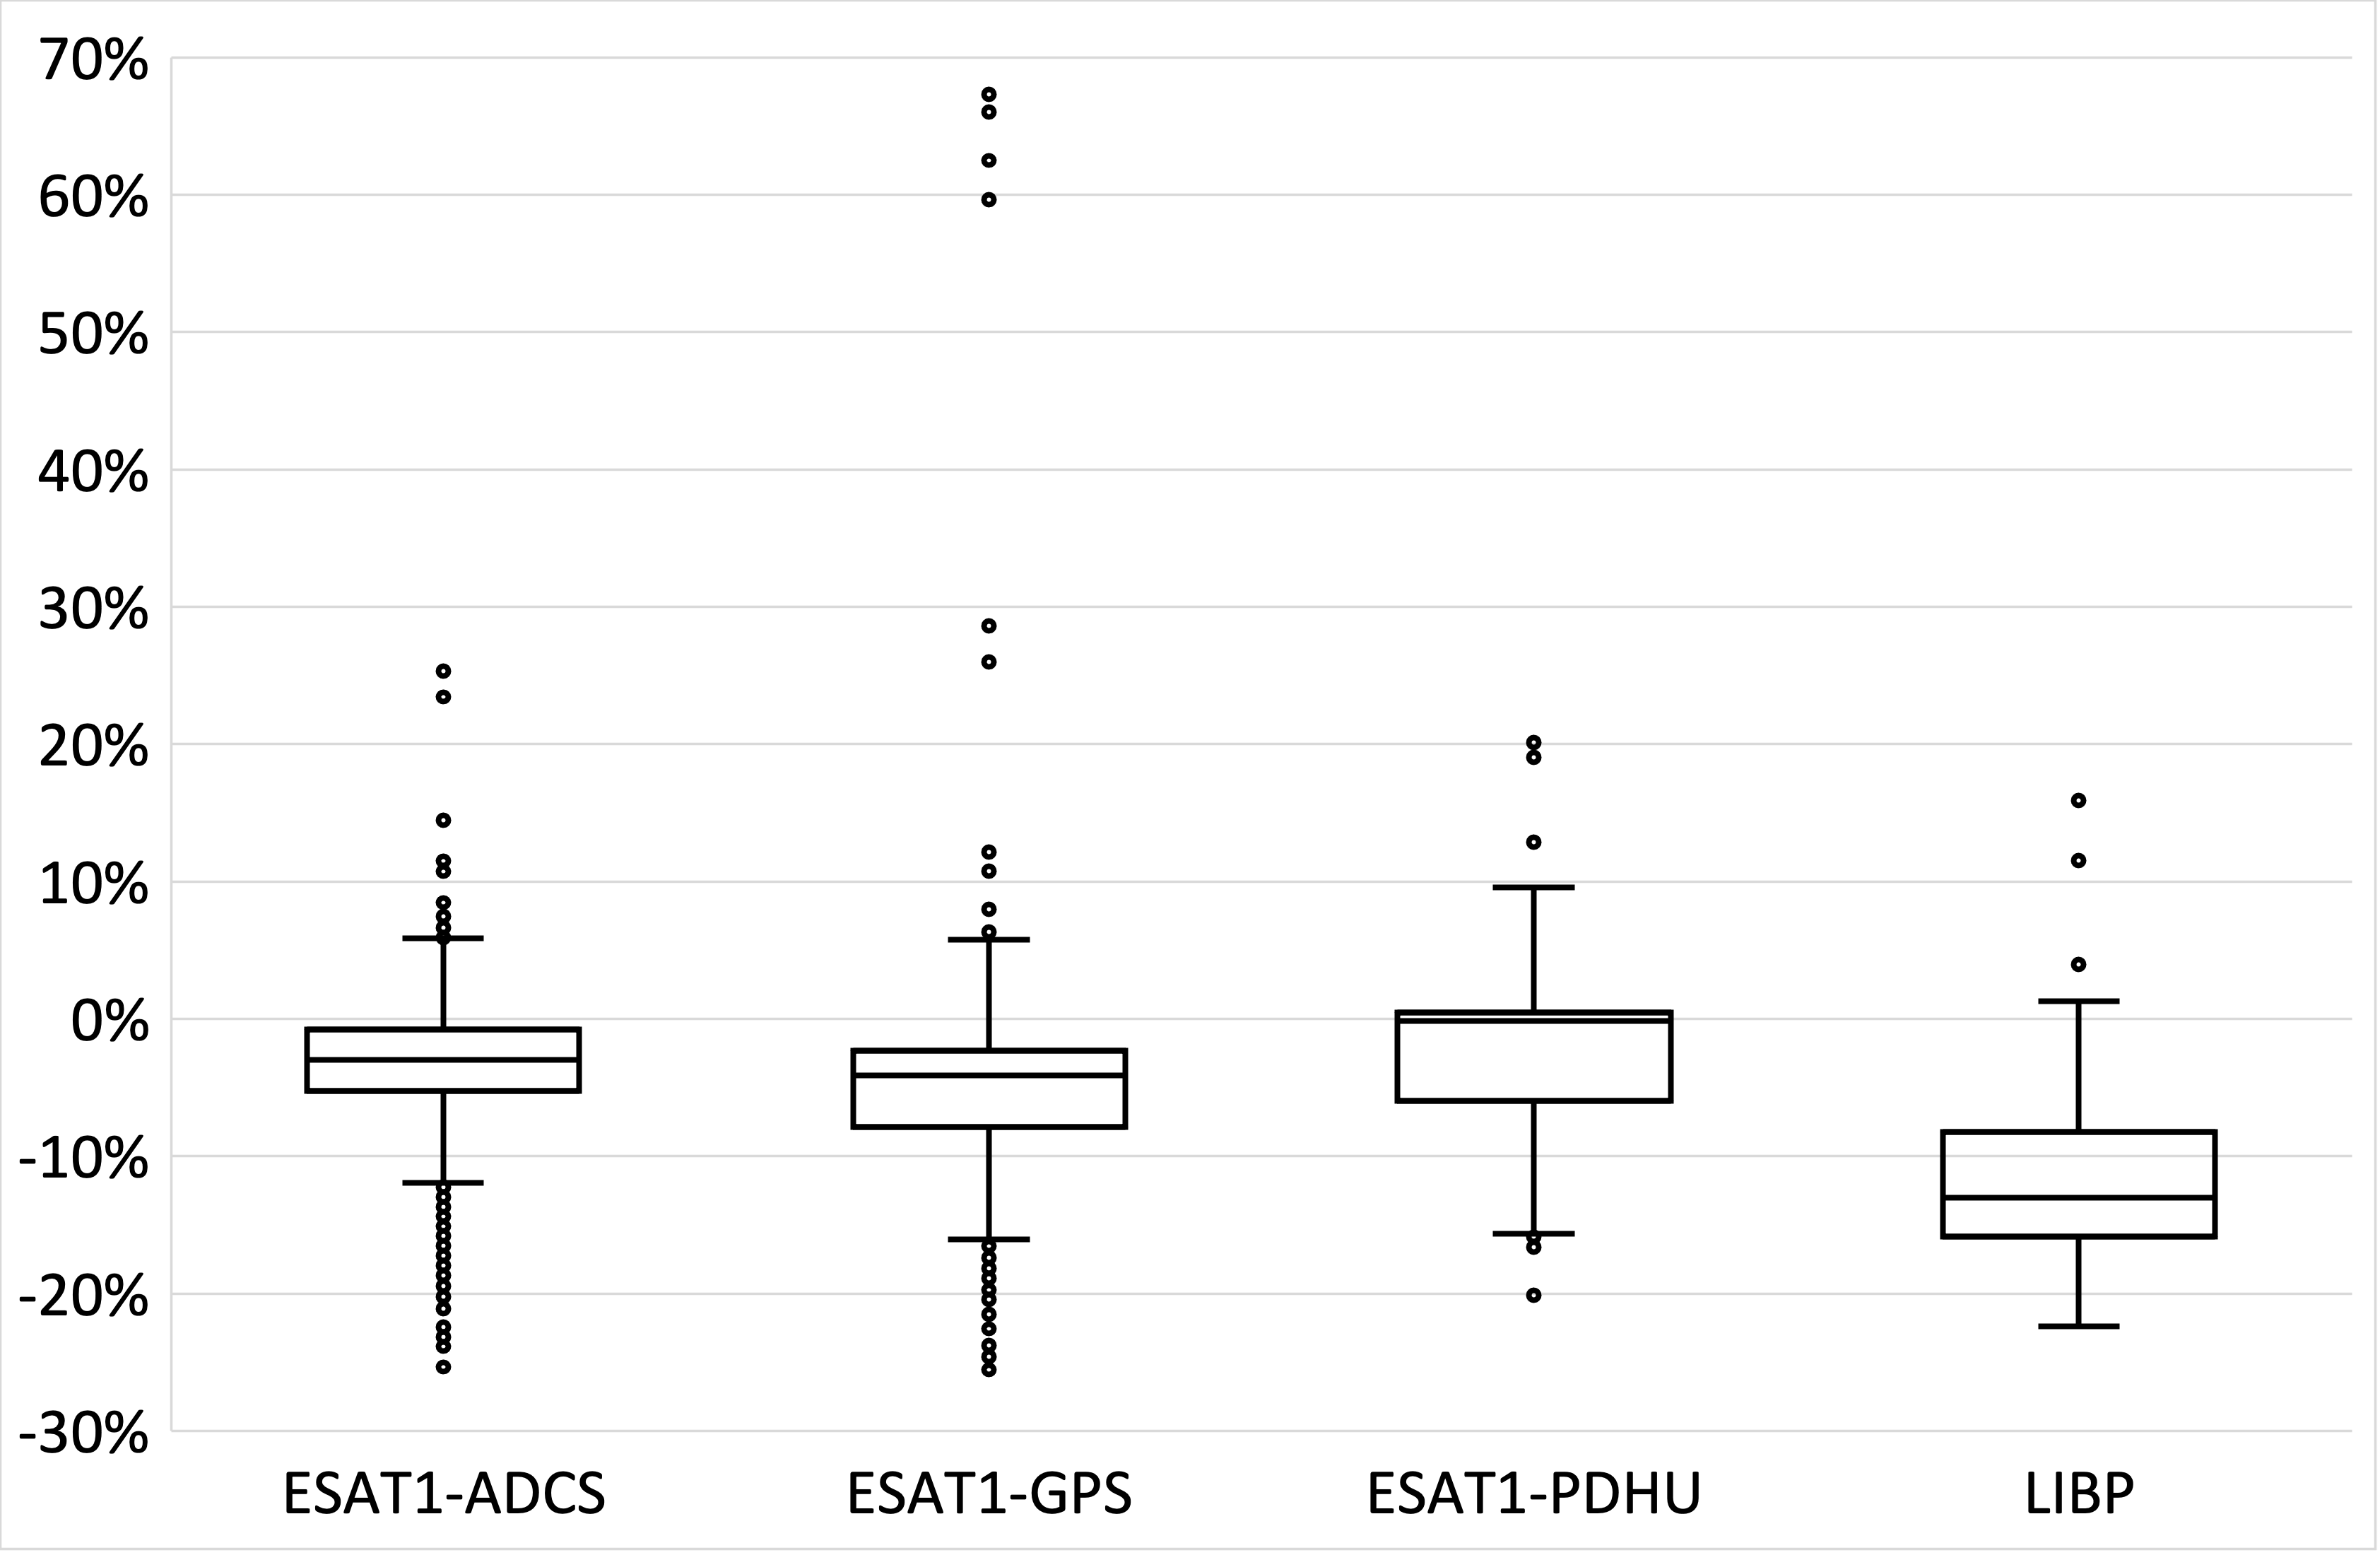
\includegraphics[width=0.8\columnwidth]{DDMA/images/overhead}
%        \caption{\APPR execution overhead per mutant.}
%        \label{fig:appr:overhead}
%    \end{figure}


% \subsection{RQ5 - Relation between data-driven and code-driven mutation analysis}

% \subsubsection*{Design and measurements}

% RQ5 aims to evaluate if data-driven mutation analysis is an alternative to code-driven analysis for a same execution cost (i.e., same number of mutants).
% Particularly, we aim to determine if data-driven mutation analysis subsumes the code-driven one when a same number of mutants is considered. Data-driven mutation analysis subsumes code-driven mutation analysis if
% the set of test cases that achieve maximal mutation analysis results for data-driven mutation analysis achieves the maximal mutation analysis results also for code-driven mutation analysis.
% %every test case that kills a data-driven mutant is guaranteed to also kill a code-driven mutant.

% Since in our context it is not possible to automatically generate 100\% mutation score we assume that the mutation analysis results achieved by the existing test suites are the maximal achievable.

% In practice, we perform an experiment in which we remove all the test cases that kill data-driven mutants and evaluate the effect on the mutation score for the code-driven mutants (hereafter, code-driven mutation score).
% More specifically, (1) we randomly select $N$ code-driven mutants (being $N$ equal to the number of data-driven mutation operations for a specific subject) generated with an extended version of SRCIRor~\cite{hariri2018srciror} from a set of source files targeting the system or sub-system under analysis. 
% (2) We execute the code-driven mutants against the test suite without the test cases killing all data-driven mutants, 
% and (3) we compute the mutation score of such set. 
% If data-driven mutation analysis subsumes code-driven mutation analysis the 
% code-driven mutation score
% shall be close to zero.
% To account for randomness we repeat the experiment 5 times.

% Similarly, we study if code-driven subsumes data-driven mutation analysis by removing all the test cases that kill code-driven mutants and evaluate the effect on the data-driven mutation analysis result. %mutation score for the data-driven mutants.

% On one hand, the nature of code-driven mutation analysis causes the technique to generate a large number of mutants (e.g., hundreds of thousands of mutants~\cite{papadakis2019mutation,zhang2013operator} can be generated for a 70K LoC system), scenario that can be worsened when considering the complexity and size of CPS software, combined with its high test execution cost. 
% On the other hand, data-driven mutation analysis simulates high level faults on interoperability of integrated components, which generates by its nature, a smaller set of mutants (i.e., between 20 and 120 mutants in our subjects).
% Consequently, a reasonable idea would be to consider data-driven mutation analysis rather than code-driven mutation analysis, because of its lower cost.

% To verify the subsumption relation, 

% for each data-driven mutant, we measure the overall number of code-driven mutants non detected when removing the test set killing such data-driven mutant.
% If the resulting distribution of non detected code-driven mutant has an average/median close ($\pm 5\%$) to the total number of originally killed code-driven mutants, means that code-driven mutation was subsumed by data-driven mutation analysis.


% we measure the overall number of code-driven mutants not detected when removing a test case killing a data-driven mutant. If the number is high, it means that data-driven mutation enable to detect more limitations than code-driven mutation.


% To do so, for every subject, and for each data-driven mutant, we remove the test cases that kill the mutant and measure how many code-driven mutants are no longer detected. Then, in a similar way, for each code-driven mutant, we remove the test cases that kill the mutant and measure how many data-driven mutants are no longer detected. 
% When comparing data-driven and code-driven approaches for a specific subject, we consider the same number of mutants (e.g., for the \ADCS subjects we generate 119 data-driven mutants, and 119 code-driven mutants).

% For the assessment of code-driven mutants on our subjects %we use MASS~\cite{}
% we performed the following steps: (1) we used a extended version of SRCIRor~\cite{hariri2018srciror} for the generation of mutants based on the test suite's code coverage, (2) we disregarded equivalent and redundant mutants based on trivial compiler optimizations~\cite{kintis2017detecting}, (3) we randomly sampled $N$ mutants from the whole set and (4) we executed the test suite against the sampled mutants. 

% We study the distribution of the code-driven mutants not detected when removing a test case killing a data-driven mutant. 
% We also study the distribution of the data-driven mutants not detected when removing a test case that kills a code-driven mutant.
% To analyze the distributions we use a t-test that enables the comparison of two distributions. 
% If both distributions have similar means, it indicates that each technique kill a set of mutants that is different from the other approach. In the case that both distribution have different means, it means that one technique kills a set of mutant that includes the set of killed mutants of the other technique.




% \subsubsection*{Results}
% \TODO{TBD}



\subsection{Threats to validity} 


%To ensure the same conditions to all mutant executions, we run each test suite in a clean instance of a virtualized environment.}

\emph{Generalizability}. We have selected industrial software systems of diverse size, tested with different types of test suites. They are developed according to space safety standards and are thus  representative of software system software adhering to safety regulations. Also, \ESAIL is larger than any other industrial system considered in the mutation analysis literature to date~\cite{Ramler2017,delgado2018evaluation,Baker2013,denisov2018mull}.
{\emph{Internal}. To minimize implementation errors, we have extensively tested our toolset; we provide both the test cases and the \APPR source code.}
{\emph{Construct}. The indicators selected for cost estimation (configured operators and LoC) are directly linked to the activities of the end-user and are thus appropriate. We leave empirical studies with human subjects to future work. To discuss overhead, we rely on test execution time, which may be affected by other factors than mutation overhead (e.g., the system behaves differently with mutated data). Dedicated benchmarks might be an alternative.}
{\emph{Conclusion}. To ensure reliability, for RQ1 and RQ2, we confirmed our findings with engineers.}

%However, we realize that the procedure we followed for the selection of pairs of mutants, only showed additional ways to improve and augment a test suite.
%For example, for the \ADCS subject, the procedure showed that two mutants from the same fault model (i.e., SunSensorTM), but targeting different data items, data item 0 and 28 respectively, are failing in the same way. This is not a sign of mutant redundancy, but an evidence that test suite should distinguish the two mutants independently, through two different test cases.
%
%This is in line with related work~\cite{}, showing that test suites should be augmented with additional test cases to make a single mutant fail.


% \subsection{RQ6 - Mutation operation coverage}

% % \subsubsection*{Design and measurements}

% % Given that CPSs are usually constrained by very %strict time limits
% % hard real-time requirements, it may make sense to limit the number of times a mutation probe is activated, to avoid interfering with real-time tasks. 

% % Depending on how often test checks (e.g., test assertions) are performed, it may make sense to reduce the number of times a mutation is performed. For example, short test cases (e.g., unit test cases) often verify every value under test, so even mutating a portion of them might lead to a test fail. 
% % Surely, by reducing the number of times a mutation is performed, we might decrease the chances of a mutant being killed.

% Because of the complexity and size of CPSs, combined with its high test execution cost, we are interested in limiting the number of times a mutation probe is activated.
% To this end, we aim to study how mutation analysis results vary when changing the proportion of data item instances to mutate. 

% % Our goal is to determine the quality of CPS test suites in terms of how often test checks are performed during test suite execution. For instance, a high quality test suite shall detect every mutated data, so in the case that a mutation is applied once, there should be a failing test case.

% Our goal is to provide guidelines for mutants sampling (i.e., the probability of executing a mutant) to determine if there exists a threshold for the sampling rate that makes it likely to detect all the limitations of a test suite.

% To do so, for each subject, we consider the three cases described in Section~\ref{sec:mutantsExecution}:

% \begin{enumerate}
%     \item The mutation is applied only once,
%     for every test case, on the first data item instance processed by the mutation probe.
%     %the mutation occurs the first time the mutant is executed.
%     \item The mutation is applied on every data item instance processed by the mutation probe.
%     \item The mutation is applied with a probability $p$, ranging from 10\% to 90\%, in steps of 10\%.
% \end{enumerate}


% %For each probability $p$ of setup (2), 
% To account for randomness, we repeat the experiment 5 times.
% %, i.e., we compute the mutation score 5 times, based on 5 executions of all mutants against the subject test suite.

% %We discuss the setup that provides the closest mutation score with respect to the mutation score obtained when mutating all the times. 

% We identify the differences between the mutation analysis results obtained across the configurations specified above and assess the significance of such differences.

% \subsubsection*{Results}
% \TODO{TBD}




% !TEX root = MAIN.tex
\clearpage
\section{Code-driven Mutation Testing (Test Suite Augmentation)}
\label{sec:testGeneration:codeDriven}

\subsection{Overview}

We address the following research questions:

\emph{RQ1. Does SEMuS scale in the context of space software?}

\emph{RQ2. Does SEMuS improve the mutation score of test suites?}

\subsection{Subjects of the Study}

To perform our experiments, we considered two software artifacts, both of them provided by the European Space Agency (ESA): ASN1SCC (or ASN.1) and MLFS.
In the case of ASN.1, the test suite is automatically generated with an approach that aims to maximize the boundary conditions of the input domain being covered. 
The Mathematical Library for Flight Software (MLFS) implements mathematical functions qualified for flight software (it complies with ECSS criticality category B).
Both test suites considered in this study characterize by high statement coverage as required by space software standards (e.g., category C software requires statement adequacy according to ECSS). MLFS test suite achieves MC/DC coverage (i.e., 100\% coverage), while ASN.1 case study achieves 99\% statement coverage.

% \TODO{to be fixed}
% \REVOCT{C-P-19}{We did not considered ESAIL in our empirical evaluation, because of the known incompatibility of clang (i.e., the compiler required by SEMuS) and ESAIL specific compilation libraries (i.e., RTEMS). More details can be found in Section~\ref{}.}

\subsection{Setup}

To address our research questions, we consider mutation analysis a precondition for our subjects; this is necessary since test generation only requires the list of live mutants (i.e., generating test inputs for all possible mutants would be far too expensive). Table~\ref{table:results:semus:ms} reports the mutation analysis results (i.e., MASS output) for the ASN.1 and MLFS subjects.

\begin{table}[htb]
\caption{Mutation scores for artifacts.}
\label{table:results:semus:ms} 
\centering
\begin{tabular}{|
@{\hspace{1pt}}p{20mm}|
@{\hspace{1pt}}>{\raggedleft\arraybackslash}p{20mm}@{\hspace{1pt}}|
>{\raggedleft\arraybackslash}p{15mm}@{\hspace{1pt}}|
>{\raggedleft\arraybackslash}p{15mm}@{\hspace{1pt}}|
 >{\raggedleft\arraybackslash}p{35mm}@{\hspace{1pt}}|
}
\hline
\textbf{Subject}&\textbf{Mutants}&\textbf{Killed}&\textbf{Live}&\textbf{Mutation Score (\%)}\\ 
\hline
$\mathit{MLFS}$&21\,375&17\,484&3\,891&81.80 \\
$\mathit{ASN.1}$&5\,323&3\,104&2\,219&58.31 \\
\hline
\end{tabular}

\end{table}

As shown in Table~\ref{table:results:semus:ms}, we apply test generation for the 3\,891 live mutants of MLFS, and for the 2\,219 live mutants of the ASN.1 subject.
For every subject, we applied the SEMuS toolset on Linux OS running on the HPC cluster of the University of Luxembourg. The HPC cluster consists of Intel Xeon E5-2680 v4 (2.4 GHz) nodes. To make our experiments feasible we executed 14 SEMuS parallel instances running on a dedicated node.

\subsection{RQ1 - Approach scalability}
\label{sec:rq1:semus}

To assess \INDEX{SEMuS} scalability we measure the execution time of each SEMuS instance. Table~\ref{table:results:semus:times} shows statistics about execution times for MLFS and the ASN.1 subjects.
Firstly, we notice is that median time taken by SEMuS to generate test inputs is the same for both case studies (i.e., 0.4 minutes). While, the mean differs for both case studies, 8.5 minutes for MLFS, and 33.4 for ASN.1 case study. Secondly, we notice that the maximum execution time is limited by the configuration we imposed in SEMuS for the symbolic search, that is, two hours.
Lastly, we notice that the total execution time of MLFS is approximately 556 hours, which can be executed on only 5.5 hours if executed with 100 HPC nodes. Similarly, the ASN.1 subject can be executed in approximately 1\,161 hours, or 11.6 hours if executed with 100 HPC nodes. In this context, even paying for the computational power of 100 HPC nodes for making test generation feasible in half a day is economically justifiable in the space software context.

    \begin{figure}[tb]
    \centering
        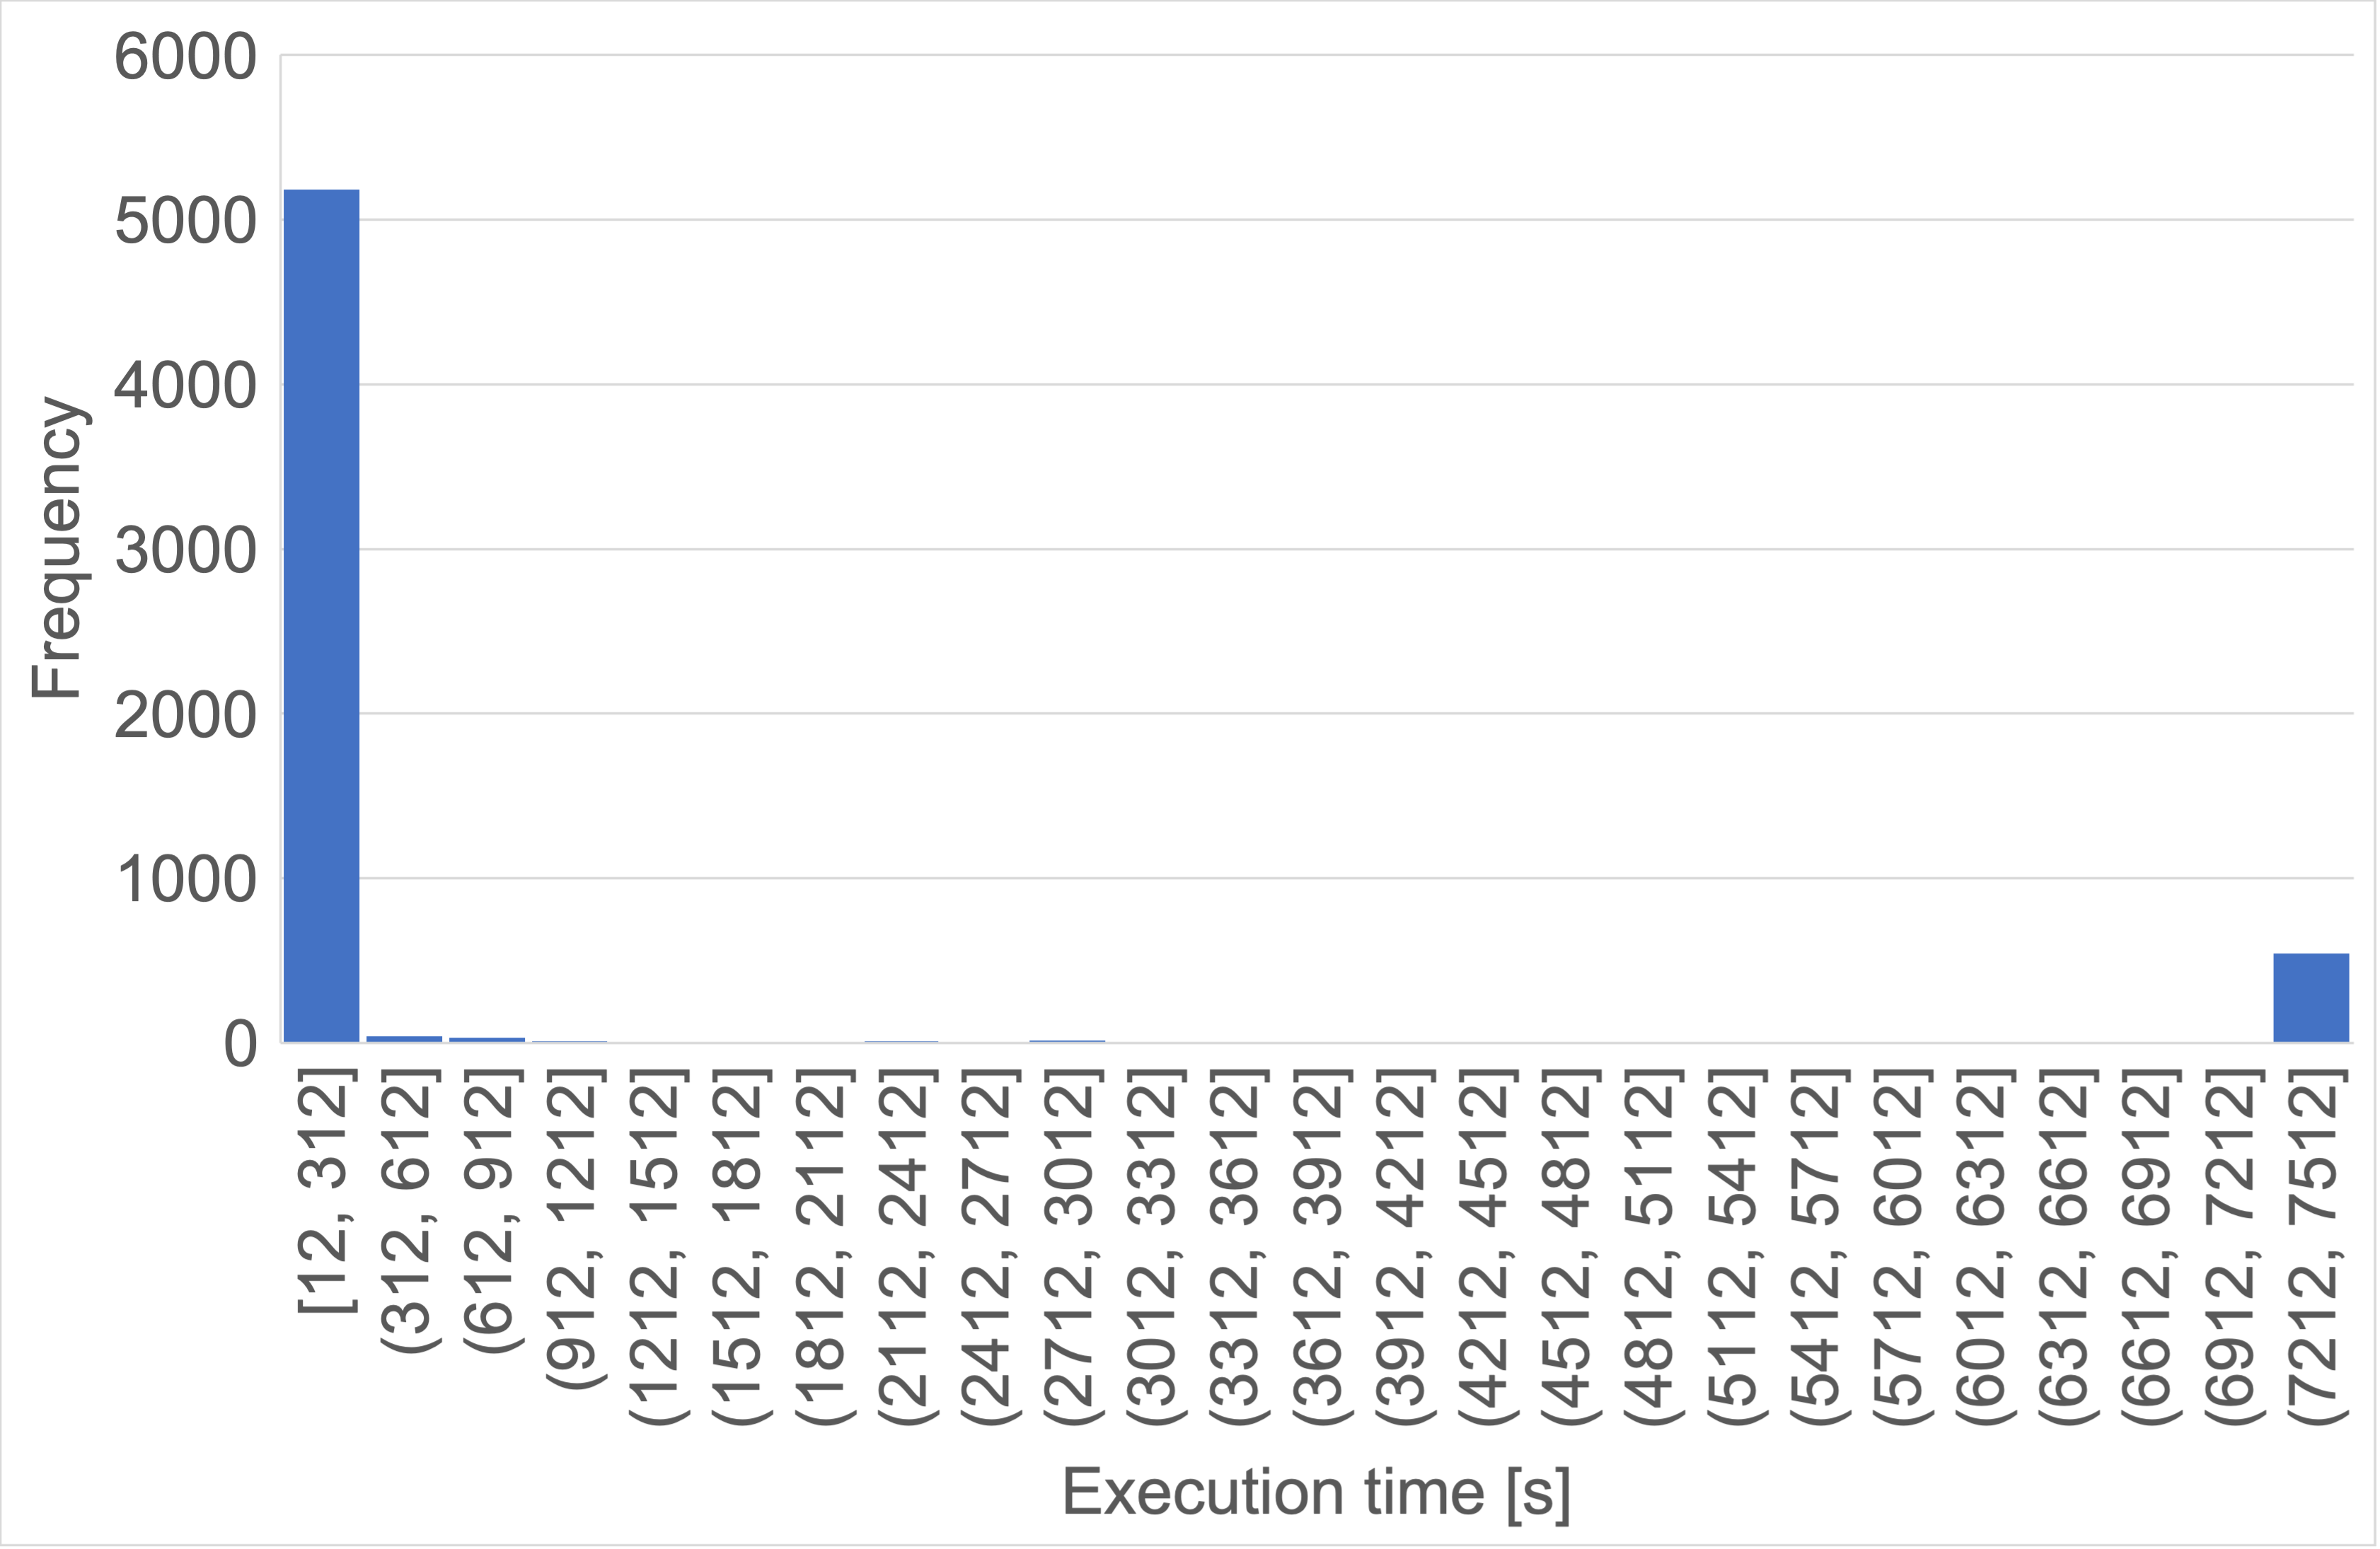
\includegraphics[width=0.7\textwidth]{images/execution_time}
        \caption{SEMuS execution time histogram.}
        \label{fig:semus:histogram_time}
    \end{figure}

\REVOCT{TDR-SUM-PABG-01}{Furthermore, we report in Figure~\ref{fig:semus:histogram_time} the histogram of the execution time of all test cases generated for both ASN.1 and MLFS. Particularly, we can see that for 5\,068 mutants (89.11\%) the test case generation time was approximately 5 minutes, and that only 545 mutants took 2 hours approximately (the maximum time configured for our experiments, which leads to test cases not being generated). In line with these results, we conclude that test generation with SEMuS scale.}


\begin{table}[htb]
\caption{SEMuS execution times.}
\label{table:results:semus:times} 
\centering
\footnotesize
\begin{tabular}{|
@{\hspace{1pt}}p{10mm}|
@{\hspace{1pt}}>{\raggedleft\arraybackslash}p{10mm}@{\hspace{1pt}}|
>{\raggedleft\arraybackslash}p{15mm}@{\hspace{1pt}}|
>{\raggedleft\arraybackslash}p{20mm}@{\hspace{1pt}}|
 >{\raggedleft\arraybackslash}p{15mm}@{\hspace{1pt}}|
 >{\raggedleft\arraybackslash}p{25mm}@{\hspace{1pt}}|
 >{\raggedleft\arraybackslash}p{15mm}@{\hspace{1pt}}|
}
\hline
\textbf{Subject}&\textbf{Min [m]}&\textbf{Max [m]}&\textbf{Median [m]}&\textbf{Mean [m]}&\textbf{Std. Deviation [m]}&\textbf{Total [m]}\\ 
\hline
$\mathit{MLFS}$&0.2&122.5&0.4&8.5&30.2&33\,348.4\\
$\mathit{ASN.1}$&0.2&121.3&0.4&33.4&54.6&69\,696.2\\
\hline
\end{tabular}

\end{table}


\subsection{RQ2 - Approach effectiveness}


To assess the approach effectiveness, we verify whether SEMuS succeeds to generate test inputs that kills non detected mutants from our subjects. We consider SEMuS effective, if the approach improves the subject mutation score.

Table~\ref{table:results:semus:testgen} shows the variations we observed in the subjects' mutation scores, the table presents the number of live mutants, the additionally killed mutants by SEMuS, the original mutation score, and the updated mutation score.
Particularly, we observe that SEMuS kills additional 1\,729 mutants for the ASN.1 subject, increasing the mutation score from 58.31\% to 90.79\%, an impressive improvement of 32,48\%.
Instead, we observe that SEMuS kills additional 697 mutants for the MLFS subject, increasing the mutation score from 81.80\% to 85.06\%, an improvement of 3,26\%.

The lower improvement observed on the MLFS could be explained by the following reasons: (1) possible presence of many equivalent mutants, (2) bugs in SEMuS fixed recently, and (3) known limitations of KLEE (i.e., the underlying test generation tool) concerning floating-point analysis. These limitations can be assessed in a follow up project.

\REVTOOL{C-P-20}{Concering ASN.1CC, SEMuS enabled us to identify a fault in the software; precisely, the ASN.1 test cases did not verify the value of the variable \emph{pErrCode} for functions \emph{\_IsConstraintValid}. The bug was fixed in commit 0917424187be2288c59ac04c804e991aed11a3fe\footnote{{https://github.com/ttsiodras/asn1scc/commit/0917424187be2288c59ac04c804e991aed11a3fe}} ). We also identified another limitation in the test suite; more precisely, the test cases for the function\emph{\_Encode} did not verify that, for the higher-level structure, the return code is zero when the parameter  \emph{bCheckConstraints} is set \emph{false} (basically, an input partition was not covered).}


\REVTOOL{C-P-20}{By definition the quality of the test cases generated by SEMuS shall be high because they kill mutants not killed by the test suite. However, such quality might be diminished by two factors (1) SEMuS erroneously determine that a mutant is killed (this shall be a sort of implementation errors that we never encountered), (2) the mutants are not representative of realistic problems. Concerning (2) we refer the reader to literature indicating that (A) achieving a high mutation score improves significantly the fault detection capability of a test suite~\cite{papadakis2018mutation}, and (B) a very high mutation score (i.e., above 0.75) ensures a higher fault detection rate than the one obtained with other coverage criteria, such as statement and branch coverage~\cite{Chekam:17}.
Based on our observations, we can claim that the generated test cases are of high quality because they (1) cover input partitions not covered by the test suite of the SUT (i.e., the second ASN.1CC case above), (2) enables us to determine  the lack of oracles in the test suite, and (3) enabled the detection of defects (i.e., the ASN.1CC bug reported above).}

For the reasons discussed above, we consider SEMuS an effective solution for test suite improvement in the context of space software.

\begin{table}[htb]
\caption{Subjects' mutation scores after test generation.}
\label{table:results:semus:testgen} 
\centering
\footnotesize
\begin{tabular}{|
@{\hspace{1pt}}p{10mm}|
@{\hspace{1pt}}>{\raggedleft\arraybackslash}p{18mm}@{\hspace{1pt}}|
>{\raggedleft\arraybackslash}p{35mm}@{\hspace{1pt}}|
>{\raggedleft\arraybackslash}p{25mm}@{\hspace{1pt}}|
 >{\raggedleft\arraybackslash}p{25mm}@{\hspace{1pt}}|
}
\hline
\textbf{Subject}&\textbf{Live Mutants}&\textbf{Additionally Killed Mutants}&\textbf{Original MS (\%)}&\textbf{Updated MS (\%)}\\ 
\hline
$\mathit{MLFS}$&3\,891&697&81.80&85.06\\
$\mathit{ASN.1}$&2\,219&1\,729&58.31&90.79\\
\hline
\end{tabular}

\end{table}


\subsubsection{Identifying test suite shortcomings with SEMuS}
\label{sec:shortcoming:semus}

To further analyze SEMuS results, we inspected manually some of the test inputs generated for the ASN.1 case study.
In particular, for the mutant \texttt{test.mut.1298.2\_1\_23.ICR.T\_INT\_IsConstraintValid} we discovered one shortcoming of the ASN.1 test suite. We introduce below detailed information about the mutant under analysis.

The original code of the mutated function, \texttt{T\_INT\_IsConstraintValid}, is shown in Listing~\ref{original_asn_code}.

\begin{lstlisting}[style=CStyle, float=t, caption=Original code., label=original_asn_code]
flag T_INT_IsConstraintValid(const T_INT* pVal, int* pErrCode) {
    flag ret = TRUE;
    (void)pVal;

    ret = ((*(pVal)) <= 50UL);
    *pErrCode = ret ? 0 : ERR_T_INT; 

    return ret;
}
\end{lstlisting}

Listing~\ref{mutant_asn_code} shows the mutated version of the function \texttt{T\_INT\_IsConstraintValid}. Particularly, the mutation operator ICR has replaced the $0$ value on line 6 with a $-1$ value.

\begin{lstlisting}[style=CStyle, float=t, caption=Mutant code., label=mutant_asn_code]
flag T_INT_IsConstraintValid(const T_INT* pVal, int* pErrCode) {
    flag ret = TRUE;
    (void)pVal;

    ret = ((*(pVal)) <= 50UL);
    *pErrCode = ret ? -1 : ERR_T_INT;

    return ret;
}
\end{lstlisting}


Listing~\ref{ktest} shows the KLEE test produced by SEMuS; we observe that SEMuS generated an input for the \texttt{pVal} argument of the function (i.e., an integer of 8 bytes).

\begin{lstlisting}[language={}, float=t, caption=Klee-test output, label=ktest]
ktest file : 'test000001.ktest'
args       : ['/MakeSym-TestGen-Input/direct/T_INT_IsConstraintValid/test.MetaMu.bc']
num objects: 2
object    0: name: b'model_version'
object    0: size: 4
object    0: data: b'\x01\x00\x00\x00'
object    1: name: b'pVal'
object    1: size: 8
object    1: data: b'\x00\x00\x00\x00\x00\x00\x00\x00'
\end{lstlisting}

SEMuS output shows that a \texttt{pVal} value equal to 0 kills the mutant. 
However, we noticed that the ASN.1 test suite already contains test cases with invocations to the \texttt{T\_INT\_IsConstraintValid} function with \texttt{pVal = 0}, in addition to \texttt{pVal = 50}.

Listing~\ref{test_code} shows an excerpt of the ASN.1 test suite, and in particular, the function that verifies the output of \texttt{T\_INT\_IsConstraintValid}. 
We manually verified the reason of \texttt{pVal=0} not being detected by the test suite. Particularly, we notice that after the invocation of the function under test, the value of \texttt{pErrCode} is never checked and it is further re-written on line 10. 

\begin{lstlisting}[style=CStyle, caption=ASN.1 test code., label=test_code]
flag T_INT_enc_dec(const T_INT* pVal, int* pErrCode, const char* filename)
{
    static T_INT decodedPDU;
    flag ret = TRUE;
    ...
            // validate decoded data
            ret = T_INT_IsConstraintValid(&decodedPDU, pErrCode); 
            if (ret) {
                ret = T_INT_Equal(pVal, &decodedPDU);
                *pErrCode = ret ? 0 : 4;
                if (ret) {
                    char buf[1024];
                    strcpy(buf, filename);
                    FILE* fp = fopen(strcat(buf,".dat"), "wb");
                    fwrite(bitStrm.buf, 1, bitStrm.count, fp);
                    fclose(fp);
                }
            }
    ...
}
\end{lstlisting}

We confirmed this shortcoming with ASN.1 engineers, who provided a solution to fix this issue.

% !TEX root = MAIN.tex
\clearpage
\section{Data-driven Mutation Testing (Test Suite Augmentation)}
\label{sec:testGeneration:dataDriven}

\STARTCHANGEDFINAL
% Empirical evaluation concerning an approach for data-driven test suite augmentation has not performed because of the lack of an automated solution (see D2). In WP4, however, we will perform an empirical evaluation of the feasibility of the proposed manual approach.

\subsection{Overview}

\DAMTE aims to address a task (i.e., test generation at system and integration level) that is particularly difficult to address with state-of-the-art technology (e.g., test generation toolsets based on symbolic execution). In particular, the test generation backend selected for adoption in FAQAS (i.e., KLEE) requires manual intervention to specify which are the inputs to select thus preventing the automated generation of a large number of test cases. For code-driven mutation testing we have addressed this issue by relying on a template generator, which is difficult to implement for data-driven test generation because the identification of the function to test is hardly to automate (given that data-driven mutation analysis targets integration and system testing, it might be either the function with the mutation probe or another one). Also, and more importantly, it requires the compilation of the whole software under analysis through LLVM, which is often not feasible. For the reasons above, it is not feasible at the current stage to automate test generation of the whole software under test; consequently,
it is not possible to perform a large scale evaluation of the approach but only to focus on its feasibility analysis.

To summarize, in our evaluation, we address the following research question:

\emph{RQ1. Is DAMTE feasible in the context of space software?}



\subsection{Subject of the study}

To perform our empirical evaluation, we considered LibParam, which is a client-server component to manage configuration parameters in cubesats.

We rely on DAMTE to generate inputs for the \PARAM client API functions. The invocation of the \PARAM client API functions with the identified inputs enables the definition of integration test cases that exchange messages between the \PARAM client and the \PARAM server. The exchanged messages include data item instances that enable the execution of mutation operations that were not covered in the DAMAt empirical evaluation (see Section~\ref{sec:testSuiteEvaluation:dataDriven}).

\subsection{Experimental Setup}

To address our research question, we consider mutation analysis as a precondition for our subject; this is necessary since test generation only requires the list of the mutation operations uncovered by the test suite. Table~\ref{table:mutationresults:damat} reports the current mutation analysis results (i.e., DAMAt output) for \PARAM.
Particularly, it can be seen that \PARAM reaches a Mutation Operation Coverage of 93.20\%, which means that only 3 operations out of 44 were not covered by the test suite.

\begin{table}[tb]
\caption{Mutation Analysis Results.}
\label{table:mutationresults:damat}
\center
\footnotesize
\begin{tabular}{|
@{\hspace{0pt}}>{\raggedleft\arraybackslash}p{24mm}@{\hspace{1pt}}|
@{\hspace{0pt}}>{\raggedleft\arraybackslash}p{12mm}@{\hspace{1pt}}|
@{\hspace{0pt}}>{\raggedleft\arraybackslash}p{12mm}@{\hspace{1pt}}|
@{\hspace{0pt}}>{\raggedleft\arraybackslash}p{17mm}@{\hspace{1pt}}|
@{\hspace{0pt}}>{\raggedleft\arraybackslash}p{12mm}@{\hspace{1pt}}|
@{\hspace{0pt}}>{\raggedleft\arraybackslash}p{12mm}@{\hspace{1pt}}|
@{\hspace{0pt}}>{\raggedleft\arraybackslash}p{12mm}@{\hspace{1pt}}|
@{\hspace{0pt}}>{\raggedleft\arraybackslash}p{12mm}@{\hspace{1pt}}|
@{\hspace{0pt}}>{\raggedleft\arraybackslash}p{12mm}@{\hspace{1pt}}|
}
\hline
\textbf{Subject} &
\textbf{\# FMs} &
\textbf{FMC} &
\textbf{\#MOs-CFM} &
\textbf{\#CMOs} &
\textbf{MOC}
&\textbf{Killed}&\textbf{Live}&\textbf{MS}
\\
\hline
\PARAM &6 &100.00\%  &   44 & 41 & 93.20\%  &        37&4&90.24\%\\
\hline
\end{tabular}

CMO=Covered Mutation Operation, MOs-CFM=Mutation Operations in covered FMs.

\end{table}

We applied DAMTE to generate test cases for mutants of the \emph{General} fault model that were not covered by the \PARAM test suite.
The \emph{General} fault model concerns the header structure of \PARAM messages sent from the \PARAM client to the \PARAM server.
%The \emph{General} fault model thus does not concerns the header structure of \emph{REPLY} messages sent from the \PARAM server to the \PARAM client.
The other fault model affected by a mutation operation not being covered is the fault model concerning \emph{REPLY} messages;  however, since such messages are generated by the server and received by the client, we cannot automatically generate them by applying test generation on the client.  More precisely, specific REPLY messages from the server can only be generated if an appropriate request is generated by the client; however, as described in D2, the automated generation of an appropriate request from the client is not feasible because of the communication channel that separates client and server.

Table~\ref{table:partial_fm} shows the specification of each analyzed mutant. It shows that the \PARAM test suite does not include input partitions covering non-nominal cases for the \emph{table ID} field (i.e., values above 20), and for the \emph{length} field (i.e., values above 180).

\begin{table}[tb]
\caption{Uncovered mutants from the General Fault Model.}
\label{table:partial_fm}
\center
\footnotesize
\begin{tabular}{|
@{\hspace{0pt}}>{\raggedleft\arraybackslash}p{28mm}@{\hspace{1pt}}|
@{\hspace{0pt}}>{\raggedleft\arraybackslash}p{16mm}@{\hspace{1pt}}|
@{\hspace{0pt}}>{\raggedleft\arraybackslash}p{15mm}@{\hspace{1pt}}|
@{\hspace{0pt}}>{\raggedleft\arraybackslash}p{11mm}@{\hspace{1pt}}|
@{\hspace{0pt}}>{\raggedleft\arraybackslash}p{14mm}@{\hspace{1pt}}|
@{\hspace{0pt}}>{\raggedleft\arraybackslash}p{14mm}@{\hspace{1pt}}|
@{\hspace{0pt}}>{\raggedleft\arraybackslash}p{10mm}@{\hspace{1pt}}|
@{\hspace{0pt}}>{\raggedleft\arraybackslash}p{20mm}@{\hspace{1pt}}|
@{\hspace{0pt}}>{\raggedleft\arraybackslash}p{16mm}@{\hspace{1pt}}|
}
\hline
\textbf{MutationOperationID} &
\textbf{FaultModel} &
\textbf{DataItem} &
\textbf{Type} &
\textbf{FaultClass} &
\textbf{Threshold} &
\textbf{Status} &
\textbf{Application} &
\textbf{Description}
\\
\hline
10&General&1&LONG&FVAT&20&LIVE&NOT\_APPLIED&table ID\\
18&General&2&LONG&FVAT&180&LIVE&NOT\_APPLIED&length\\
\hline
\end{tabular}

\end{table}

For the generation of missing inputs we used KLEE 2.3 with LLVM 9.0.1. We performed our experiments on a MacBook Pro with 2,3 GHz 8-Core Intel Core i9.

Since KLEE requires the SUT to be compiled with clang to produce the bitcode files (i.e., KLEE input) and \PARAM is not originally expected to be compiled with clang but gcc,
%, and also to avoid incompatibilities with the original compiler (i.e., gcc).
we evaluated two different approaches for compiling \PARAM. First, we compiled the whole library into one bitcode file, to minimize the risk of imprecise results (i.e., KLEE might simulate the output of a function if the implementation of it is not provided). Second, we isolated the function under test in a different source file, so that only the required functions are compiled with clang. In the following, we discuss both the feasibility of each compilation strategy and the quality of the identified test inputs.

To drive test generation with KLEE, as presented in D2, we rely on a test template that initializes the required data structures and invokes the function under test.
The generation of the inputs that cover the mutant is enabled by the use of the DAMAt mutation probe API configured for test generation instead of mutation.
In particular, following the procedure described in D2, we add a call to function \texttt{\_FAQAS\_mutate} in the code of the \PARAM client. In the context of test generation, function \texttt{\_FAQAS\_mutate} instead of mutating the data includes a reachability assertion (i.e., \emph{assert(false)}) that forces the generation of a specific data item instance (see D2).

\subsection{RQ1 - Feasibility}


% (i.e., the uncovered input partition for a specific data item).

In the following, we discuss the procedure and the results obtained when applying DAMTE to LibParam using the two different configurations introduced above  (i.e., \emph{full compilation of \PARAM} and \emph{isolating the function under test}).

\subsubsection{Full compilation of \PARAM}

We modified the WAF compilation configuration file, and enabled clang as the main compiler of the library. This was done by replacing \texttt{conf.load('gcc')} by \texttt{conf.load('clang')} in the \url{tools/buildtools/waftool/gs_gcc.py} script.
Then, we proceeded by adding the following compiler arguments to the configuration file \url{tools/buildtools/gs/buildtools/compiler_settings.json}:


\begin{lstlisting}[style=CStyle]
"CFLAGS": ["-c", "-std=gnu99", "-m64", "-g", "-Xclang" , "-disable-O0-optnone", "-save-temps"],
\end{lstlisting}

Note that the parameter \texttt{-save-temps} forces clang to produce \texttt{bc} files along with the object files.

After generating all the \texttt{bc} files, we linked together into one bitcode file with the following command:

\begin{lstlisting}[style=CStyle]
$ llvm-link-9 *.bc -o libparam.exe
\end{lstlisting}

We processed then \texttt{libparam.exe} with KLEE with the following command:

\begin{lstlisting}[style=CStyle]
$ klee --libc=uclibc --posix-runtime --external-calls=all libparam.exe
\end{lstlisting}

However, with the approach described above, KLEE throws several errors about missing function implementations. These errors occur because the WAF clang module outputs all the bitcode files into a same folder without respecting the original compiler organization (i.e., the object files are stored in the same structure of the source code). Since \PARAM contains multiple source files having the same name but different content (i.e., source code), object files without the required definitions may overwrite the ones without them; consequently, the LLVM linker generates an executable including only a subset of the required objects, which leads to errors during the execution of KLEE. A possible solution consists of extending the WAF clang module to store bitcode files appropriately - it will be evaluated in the maintenance period of the project.


\subsubsection{Isolating the function under test}

In this setup, we isolated the function under test along its dependencies and copied them into a same test template source file. Below, we describe the output observed for the two data items targeted by mutation, i.e.,
\emph{table ID} and \emph{length}.


\paragraph{Table ID}\

When generating inputs for \texttt{tableID}, we have first identified the API command that generates messages including the table ID. As indicated in D2, we selected function
\texttt{gs\_rparam\_get\_array}. Then we have identified a higher-level function that relies on function
\texttt{gs\_rparam\_get\_array}; although function \texttt{gs\_rparam\_get\_array} can be directly targeted in test cases, invoking a higher-level function is easier for an engineer (less parameters are required).
Finally, we have included in the test template all these functions and their dependencies, which are \texttt{gs\_rparam\_get}, and \texttt{csp\_hton16}.
%which are necessary for correctly running \texttt{gs\_rparam\_get\_string}.

Listing~\ref{get_array} shows the source code for the function \texttt{gs\_rparam\_get\_array} with the mutation probe that enables the reachability analysis.
%so that KLEE can generate an input for the uncovered mutation operations (e.g., FVAT for table ID).

\begin{lstlisting}[style=CStyle,float=t, caption=Instrumented code for function gs\_rparam\_get\_array., label=get_array]
gs_error_t gs_rparam_get_array(uint8_t node,
                               gs_param_table_id_t table_id,
                               uint16_t addr,
                               gs_param_type_t type,
                               uint16_t checksum,
                               uint32_t timeout_ms,
                               void * value,
                               size_t value_element_size,
                               size_t array_size)
{
    /* Calculate length */
    gs_rparam_query_t * query;
    const size_t query_payload_size = sizeof(query->payload.addr[0]) * array_size;
    const size_t query_size = RPARAM_QUERY_LENGTH(query, query_payload_size);
    const size_t reply_payload_element_size = value_element_size + sizeof(query->payload.addr[0]);
    const size_t reply_payload_size = reply_payload_element_size * array_size;
    const size_t reply_size = RPARAM_QUERY_LENGTH(query, reply_payload_size);

    query = alloca(reply_size);
    query->action = RPARAM_GET;
    query->table_id = table_id;
    query->checksum = csp_hton16(checksum);
    query->seq = 0;
    query->total = 0;
    for(unsigned int i = 0; i < array_size; i++) {
        query->payload.addr[i] = csp_hton16(addr + (value_element_size * i));
    }
    query->length = csp_hton16(query_payload_size);

    FaultModel *fm_General = _FAQAS_General_FM();
    unsigned long long int v_General[6];

    v_General[0] = (unsigned long long int) query->action;
    v_General[1] = (unsigned long long int) query->table_id;
    v_General[2] = (unsigned long long int) query->length;
    v_General[3] = (unsigned long long int) query->checksum;
    v_General[4] = (unsigned long long int) query->seq;
    v_General[5] = (unsigned long long int) query->total;

    _FAQAS_mutate(v_General,fm_General);

    return GS_OK;
}
\end{lstlisting}



Listing~\ref{get_string} shows the implementation of the test template for driving the test generation for the function \texttt{gs\_rparam\_get\_string}. Particularly, it can be seen how \texttt{tableID} is made symbolic by the KLEE API function \texttt{klee\_make\_symbolic}. Then, the function under test is called with concrete parameters and the symbolic one; concrete parameters match the one in other test cases of the \PARAM test suite.

Note that the function \texttt{gs\_rparam\_get\_string} calls \texttt{gs\_rparam\_get}, which, in turn, invokes the instrumented \\
function \texttt{gs\_rparam\_get\_array}.

\begin{lstlisting}[style=CStyle,float=t, caption=Test template for function gs\_rparam\_get\_string., label=get_string]
int main(void) {
    // a little hack - this is next element, we use it check for overwrite and missing 0 termination
    memset(alltypes_mem.string_A, 'Z', sizeof(alltypes_mem.string_A));
    alltypes_mem.string_A[0][1] = 0;

    char buf[GS_TEST_ALLTYPES_STRING_LENGTH + 10];

    // get max size - no 0 termination
    memset(alltypes_mem.string, 'B', sizeof(alltypes_mem.string));
    memset(buf, 'A', sizeof(buf));
    buf[GS_TEST_ALLTYPES_STRING_LENGTH + 1] = 0;

    uint8_t tableID;
    klee_make_symbolic(&tableID, sizeof(tableID), "tableID");
    gs_rparam_get_string(CSP_NODE, tableID, GS_TEST_ALLTYPES_STRING, GS_RPARAM_MAGIC_CHECKSUM, 1000, buf, GS_TEST_ALLTYPES_STRING_LENGTH);

    return 0;
}
\end{lstlisting}

To compile the isolated functions along with the test template, we use the KLEE compilation arguments (i.e., \texttt{-g -Xclang -disable-O0-optnone -c -emit-llvm}) through the following command:

\begin{lstlisting}[style=CStyle]
$ /usr/bin/clang -std=gnu99 -m64 -g -Xclang -disable-O0-optnone -c -emit-llvm -Wall -Wextra -Wshadow -Wcast-align -Wwrite-strings -Wno-unused-parameter -Wall -Wextra -Wshadow -Wcast-align -Wwrite-strings -Wno-unused-parameter -Wno-unused-parameter -Iinclude -I../include -I__root__/opt/libparam/lib/libgscsp/lib/libcsp/include -I../../../lib/libgscsp/lib/libcsp/include -I__root__/opt/libparam/lib/libgscsp/lib/libutil/include -I../../../lib/libgscsp/lib/libutil/include -I__root__/opt/libparam/lib/libgscsp/lib/libutil/include/gs -I../../../lib/libgscsp/lib/libutil/include/gs -I__root__/opt/libparam/lib/libgscsp/lib/libutil/include/deprecated -I../../../lib/libgscsp/lib/libutil/include/deprecated -I__root__/opt/libparam/lib/libgscsp/lib/libutil/include/deprecated/gs/gosh -I../../../lib/libgscsp/lib/libutil/include/deprecated/gs/gosh -I__root__/opt/libparam/lib/libgscsp/include -I../../../lib/libgscsp/include -I__root__/opt/libparam/lib/libparam_client/include -I../../../lib/libparam_client/include -I__root__/opt/libparam/lib/libparam_client/include/deprecated -I../../../lib/libparam_client/include/deprecated -I__root__/opt/libparam/lib/libparam_client/include/deprecated/param -I../../../lib/libparam_client/include/deprecated/param -I__root__/opt/libparam/include -I../../../include -I__root__/opt/libparam/include/deprecated -I../../../include/deprecated -Iinclude -DSTRING_1="string 1" -DFALSE=false -DELEVEN=11 -DZERO_POINT_ZERO=0.0 -DMUTATIONOPT=10 ../main_table_id.c
\end{lstlisting}

Listing~\ref{klee_damte} shows the corresponding KLEE output for the variable \emph{tableID}. In particular, it shows that the  value that enables executing the FVAT mutation operation is the value \emph{21} assigned to \emph{tableID}. In this case, we can see that DAMTE provides the expected results (i.e., a vaue above 20). Please note that despite having a name that is similar to the data item to be mutated (i.e., \emph{query->table\_id}), the variable \emph{tableID} is not processed directly by the mutation analysis tool but it is first copied into the message data structure, which exemplifies the case of KLEE generating an input that drives (after further computation) the generation of the required messages.
%which shows that KLEE may handle the identification of inputs that lead to the definition of correctly for simple variables that are directly processed by the function.

\begin{lstlisting}[style=CStyle,float=t, caption=KLEE output for the variable tableID., label=klee_damte]
object 1: name: 'tableID'
object 1: size: 1
object 1: data: b'\x15'
object 1: hex : 0x15
object 1: int : 21
object 1: uint: 21
object 1: text: .
\end{lstlisting}

\paragraph{length}\

To generate test cases that enable executing the operator affecting the \texttt{length} message item, we introduced the test template used in Listing~\ref{get_string}. In this case, we directly test the function \texttt{gs\_rparam\_get\_array} using \texttt{value\_size} as a symbolic value because function \emph{gs\_rparam\_get\_string} uses a constant value for variable \texttt{value\_size} (and therefore cannot enable test generation).

\begin{lstlisting}[style=CStyle,float=t, caption=Test template for function gs\_rparam\_get\_array.]
int main(void) {
    uint8_t buf[1000];
    memset(buf, 0, sizeof(buf));
    size_t value_size;
    klee_make_symbolic(&value_size, sizeof(value_size), "value_size");
    gs_rparam_get_array(CSP_NODE, GS_TEST_ALLTYPES_TABLE_ID, GS_TEST_ALLTYPES_UINT8_A(0), PARAM_UINT8, GS_RPARAM_MAGIC_CHECKSUM, 1000,
                                              &buf, sizeof(uint8_t), value_size);
    return 0;
}
\end{lstlisting}

Unfortunately, the execution of KLEE leads to an error stating that line 19 of Listing~\ref{get_array} produces a memory error because the symbolic value is used to  specify the dimension of a memory buffer to be allocated. The concretized symbolic value is usually assigned with a value equal to zero, which leads to an out-of-bound error; this is a known limitation of KLEE\footnote{See for example https://github.com/klee/klee/issues/1227}.
%most probably because the tool has concretized a huge value for the \texttt{alloca} function.
In this case, we can see that DAMTE does not work properly when the variable to be tested represents memory size.

Overall, we conclude that the DAMTE approach may be feasible; however, it requires some manual effort for the configuration and execution of test cases which may limit its usefulness. The first step towards its large scale applicability is the improvement of underlying test generation tools and compiler procedures, such changes will facilitate DAMTE application to large projects without the need for manually creating test template files with dependencies.

\begin{lstlisting}[style=CStyle,float=t, caption=KLEE error output, label=klee_error]
KLEE: NOTE: Using POSIX model: /tmp/klee_build90stp_z3/runtime/lib/libkleeRuntimePOSIX64_Debug+Asserts.bca
KLEE: NOTE: Using klee-uclibc : /tmp/klee_build90stp_z3/runtime/lib/klee-uclibc.bca
KLEE: output directory is "/opt/libparam/tst/rparam4_llvm/build/klee-out-1"
KLEE: Using STP solver backend
KLEE: WARNING: executable has module level assembly (ignoring)
KLEE: WARNING ONCE: calling external: syscall(16, 0, 21505, 94391800950288) at klee_src/runtime/POSIX/fd.c:1007 10
KLEE: WARNING ONCE: Alignment of memory from call "malloc" is not modelled. Using alignment of 8.
KLEE: WARNING ONCE: calling __klee_posix_wrapped_main with extra arguments.
KLEE: NOTE: found huge malloc, returning 0
KLEE: ERROR: ../main_length.c:250: concretized symbolic size
KLEE: NOTE: now ignoring this error at this location
KLEE: ERROR: ../main_length.c:251: memory error: out of bound pointer
KLEE: NOTE: now ignoring this error at this location
KLEE: WARNING ONCE: Alignment of memory from call "realloc" is not modelled. Using alignment of 8.
\end{lstlisting}

\ENDCHANGEDFINAL


\ENDCHANGEDWPT

% !TEX root = MAIN.tex
\clearpage

\section{Summary of FAQAS Validation Results}
\label{sec:summary:results}

In this section, we report the summary of results for the FAQAS framework. In particular, for each FAQAS approach, we provide a table with the main output of the technique (e.g., mutation score, number of test cases generated).

\subsection{Code-driven mutation analysis}

\begin{table}[htb]
\caption{Code-driven mutation analysis results: MASS mutation score.}
\label{table:results:mass} 
\small
\centering
\begin{tabular}{|
>{\arraybackslash}p{54mm}@{\hspace{1pt}}|
>{\raggedleft\arraybackslash}p{40mm}@{\hspace{1pt}}|
}
\hline
\textbf{Subject}&\textbf{MASS Mutation Score (\%)}\\
\hline

\SAIL{}$_{S}$ (System test suite)&65.95\\

\SAIL{}$_{S}$ (Unit+System test suite)&70.56\\

\GCSP{}&70.92\\
\PARAM{}&85.95\\

\UTIL{}&84.41\\
\MLFS{}{}&93.49\\
% K: 3104 L: 2219-1480=739 T: 5323-1480=3843
ASN1SCC&80.77\\
\hline
$\textbf{Average}$&78.86\\
\hline
\end{tabular}

\end{table}

Table~\ref{table:results:mass} introduces the code-driven mutation analysis results. 


\subsection{Code-driven mutation testing (test suite augmentation)}

\begin{table}[htb]
\caption{Test suite augmentation results.}
\label{table:results:test-gen} 
\centering
\footnotesize
\begin{tabular}{|
@{\hspace{1pt}}p{10mm}|
@{\hspace{1pt}}>{\raggedleft\arraybackslash}p{18mm}@{\hspace{1pt}}|
>{\raggedleft\arraybackslash}p{35mm}@{\hspace{1pt}}|
>{\raggedleft\arraybackslash}p{25mm}@{\hspace{1pt}}|
 >{\raggedleft\arraybackslash}p{25mm}@{\hspace{1pt}}|
}
\hline
\textbf{Subject}&\textbf{Live Mutants}&\textbf{Additionally Killed Mutants}&\textbf{Original MS (\%)}&\textbf{Updated MS (\%)}\\ 
\hline
$\mathit{MLFS}$&3\,891&697&81.80&85.06\\
$\mathit{ASN.1}$&2\,219&1\,729&58.31&90.79\\
$\mathit{ESAIL_S}$&1\,041&NA&70.56&NA\\
% additionally killed: clock 2 error 4 timestamp 6 memory 21
$\mathit{Libutil}$&4\,198&35&81.80&81.96\\
\hline
\end{tabular}

\end{table}

Table~\ref{table:results:test-gen} introduces the code-driven mutation testing results; in particular, the number of mutants additionally killed by SEMuS, and the mutation score of the test suite including the new test cases generated by SEMuS.


\subsection{Data-driven mutation analysis}

\begin{table}[htb]
\caption{Data-driven mutation analysis results.}
\label{table:results:data-driven} 
\center
\footnotesize
\begin{tabular}{|
@{\hspace{0pt}}>{\raggedleft\arraybackslash}p{24mm}@{\hspace{1pt}}|
@{\hspace{0pt}}>{\raggedleft\arraybackslash}p{12mm}@{\hspace{1pt}}|
@{\hspace{0pt}}>{\raggedleft\arraybackslash}p{12mm}@{\hspace{1pt}}|
@{\hspace{0pt}}>{\raggedleft\arraybackslash}p{18mm}@{\hspace{1pt}}|
@{\hspace{0pt}}>{\raggedleft\arraybackslash}p{12mm}@{\hspace{1pt}}|
@{\hspace{0pt}}>{\raggedleft\arraybackslash}p{12mm}@{\hspace{1pt}}|
@{\hspace{0pt}}>{\raggedleft\arraybackslash}p{12mm}@{\hspace{1pt}}|
@{\hspace{0pt}}>{\raggedleft\arraybackslash}p{12mm}@{\hspace{1pt}}|
@{\hspace{0pt}}>{\raggedleft\arraybackslash}p{12mm}@{\hspace{1pt}}|
}
\hline
\textbf{Subject} & 
\textbf{\# FMs} & 
\textbf{FMC} & 
\textbf{\#MOs-CFM} & 
\textbf{\#CMOs} & 
\textbf{MOC}  
&\textbf{Killed}&\textbf{Live}&\textbf{MS}
\\
\hline

\ADCS &10 &90.00\%   & 135 & 100 & 74.00\%   &    45&55&45.00\%\\
\GPS &1 &100.00\%    &  23  &  22 & 95.65\%    &      21&1&95.45\%\\
\PDHU &3 &100.00\%  &   29 & 24 & 82.76\%   &     24&0&100.00\%\\
\PARAM &6 &100.00\%  &   80 & 73 & 91.25\%  &        28&45&38.36\%\\


\hline

\end{tabular}

FM=Fault Model, FMC=Fault Model Coverage, MOs-CFM=Mutation Operations in covered FMs,
CMO=Covered Mutation Operation, MOC=Mutation Operation Coverage, Killed=Number of mutants killed by the test suite, Live=Number of mutants not killed by the test suite, MS=Mutation Score.

\end{table}


Table~\ref{table:results:data-driven} shows the mutation analysis results of DAMAT, our data-driven mutation analysis technique. For each subject, we provide information about the fault model coverage, the mutation operation coverage, and the mutation score of the technique.




\newpage

\appendix


\chapter{Data-driven Fault Models}
\label{appendix:FMS}

This appendix provides descriptive specifications of the fault models used in our experiments for data-driven mutation analysis. Also, it provides the tabular fault models used as input for our toolset. Since the test suite under analysis exercises a subset of the functionalities provided by the components considered for our empirical evaluation, the tabular specifications (i.e., the input for our toolset) contain a smaller set of fault models than the descriptive specifications.

\clearpage

\section{ESAIL-ADCS Fault Model Description}

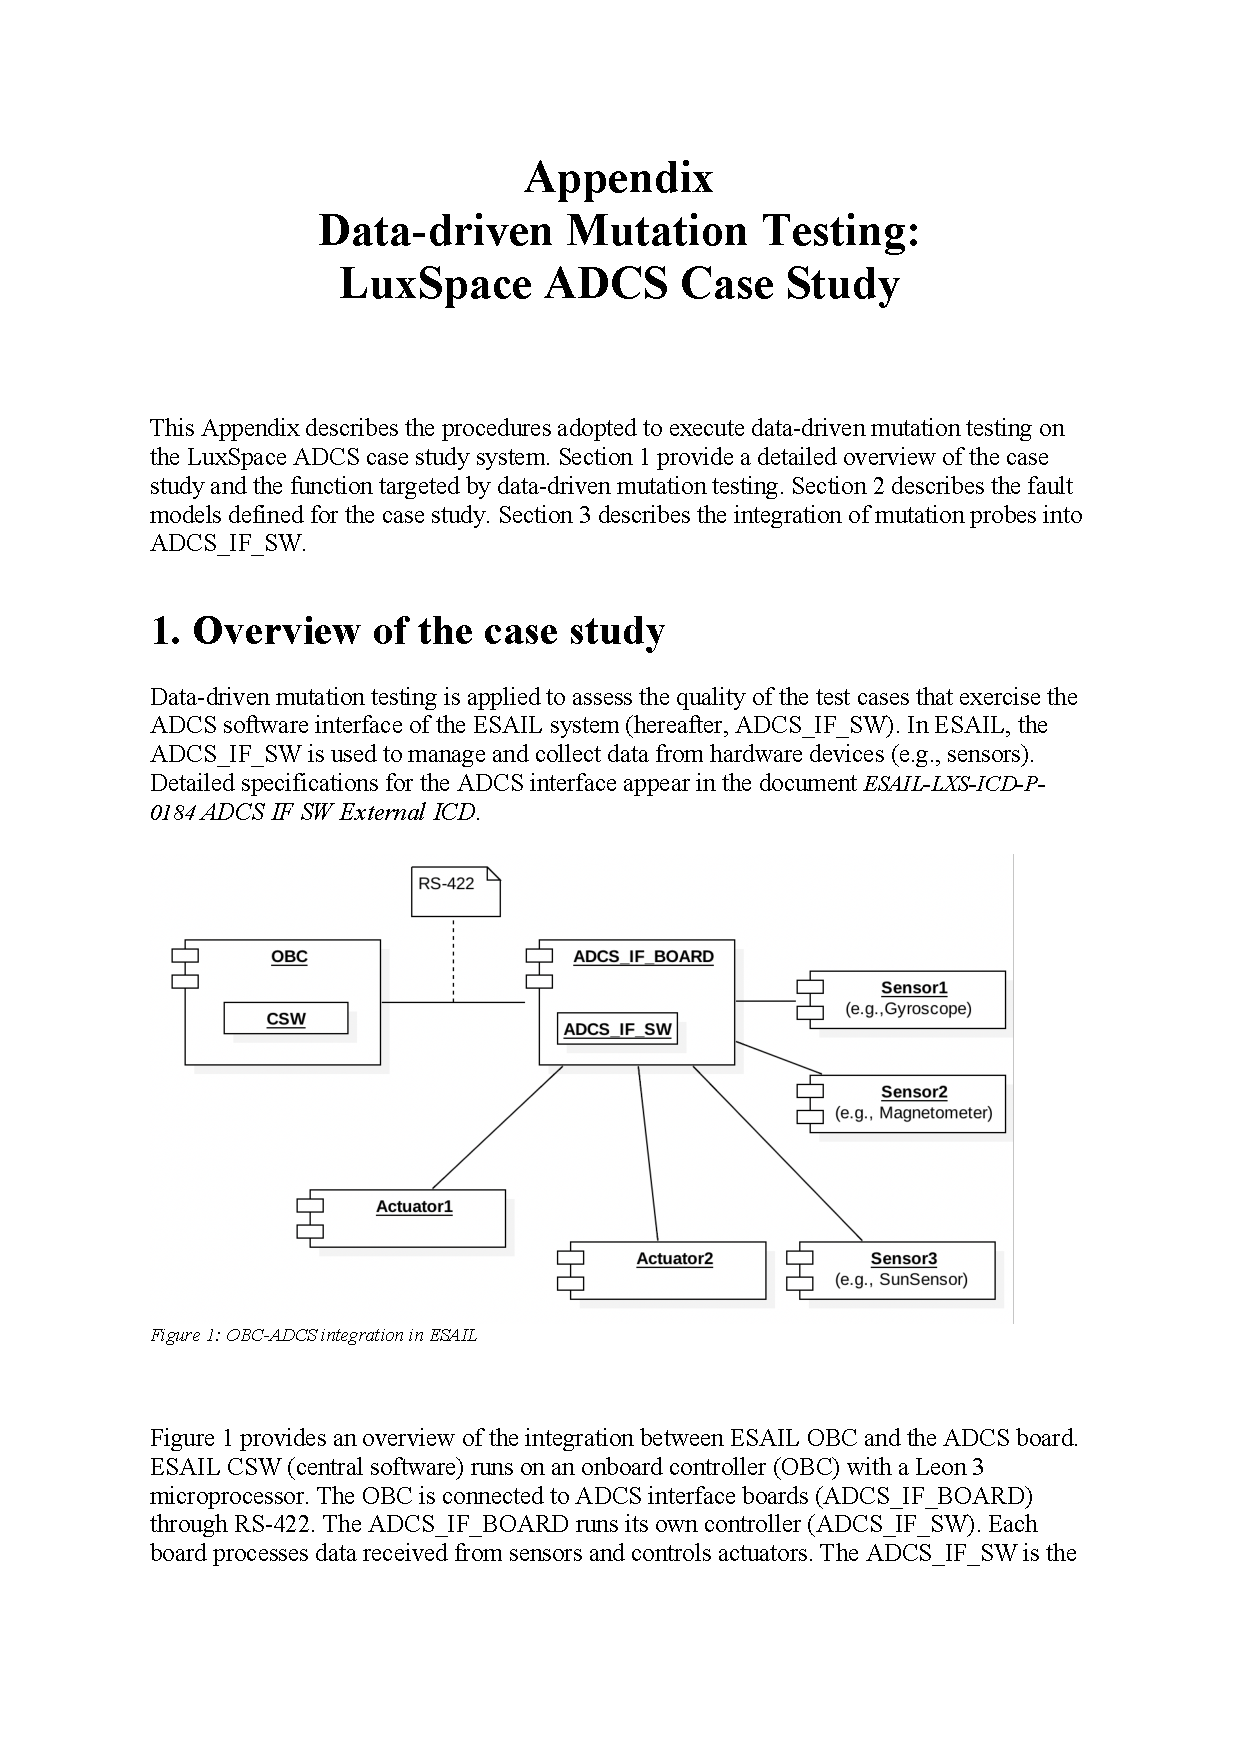
\includepdf[pages=-,scale=0.9,offset=0mm -75]{faultModels/ESAIL_ADCS_FaultModel_current_version.pdf}

\section{ESAIL-GPS Fault Model Description}

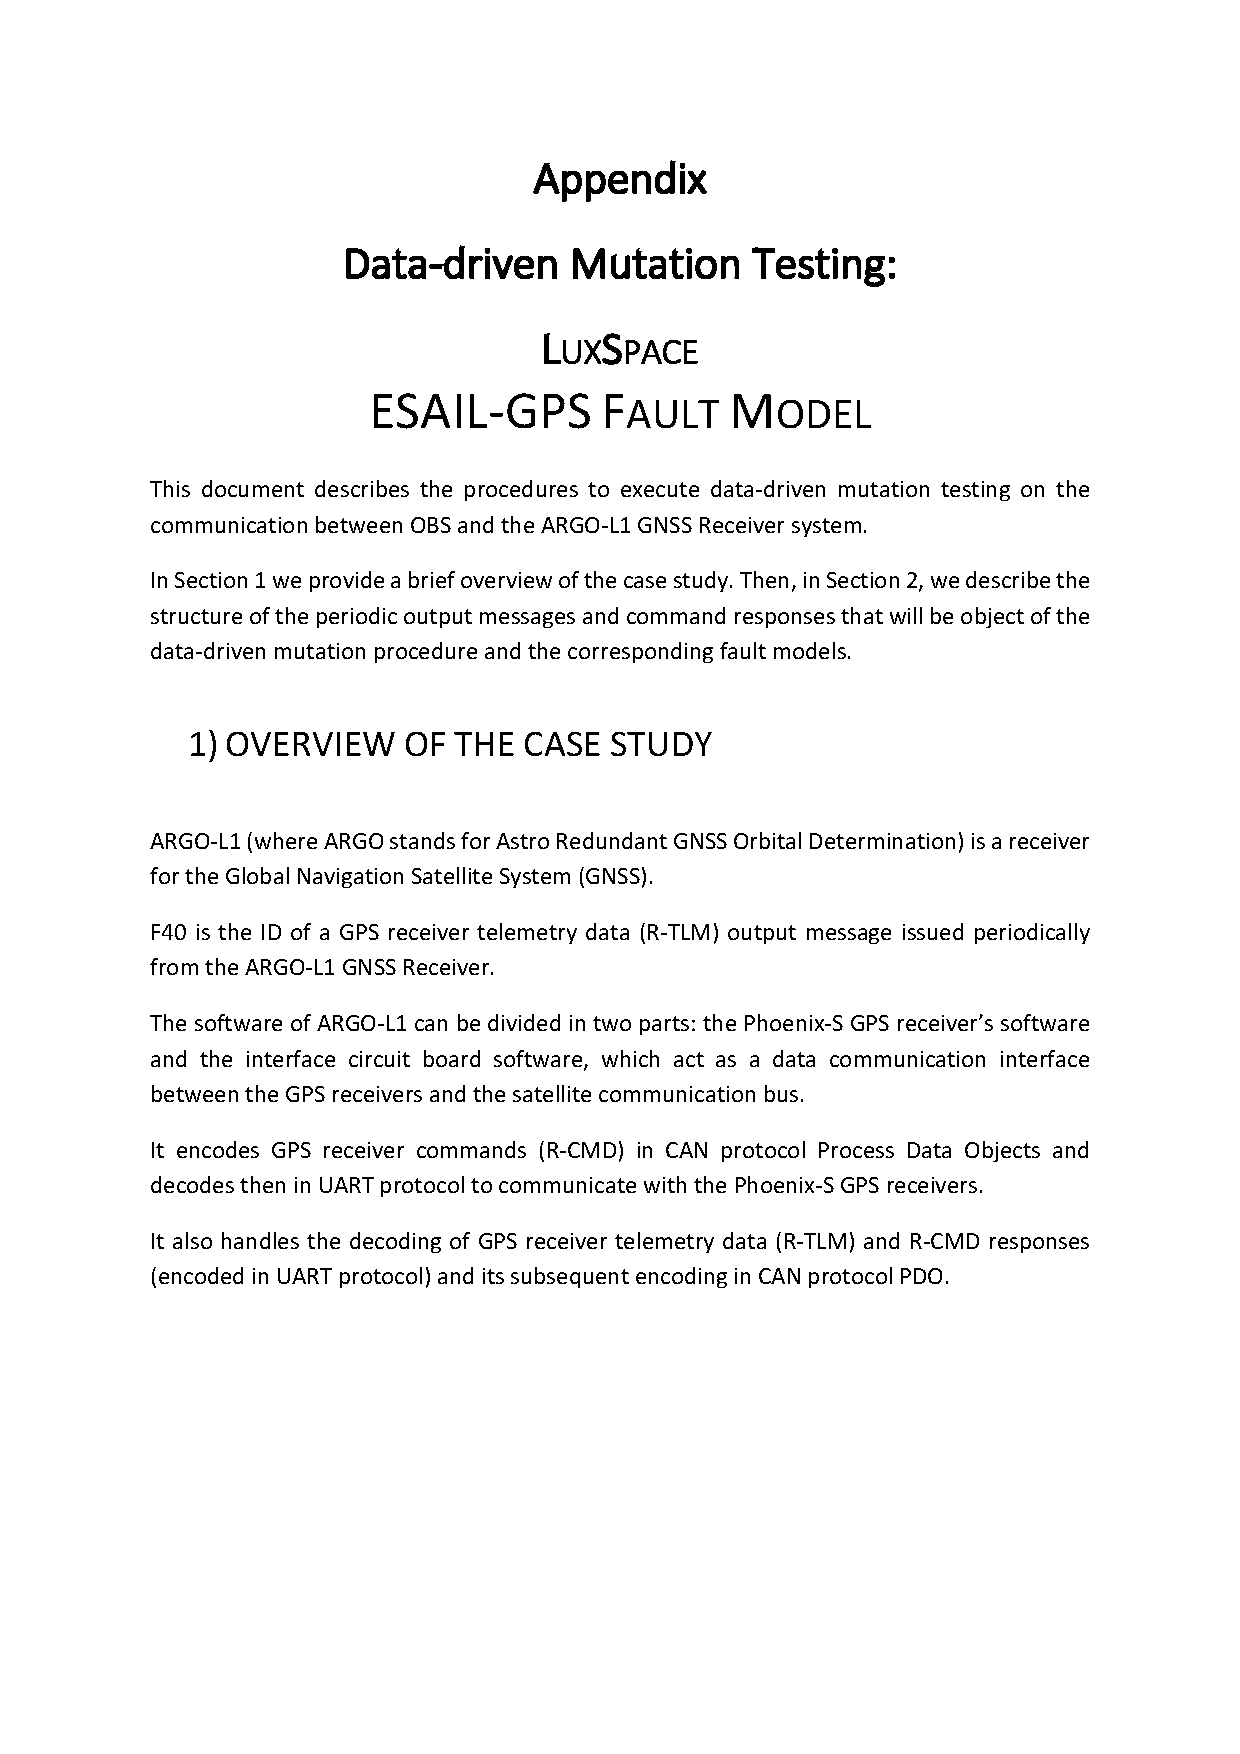
\includepdf[pages=-,scale=0.9,offset=0mm -75]{faultModels/ESAIL_GPS_Fault_Model.pdf}

\section{ESAIL-PDHU Fault Model Description}

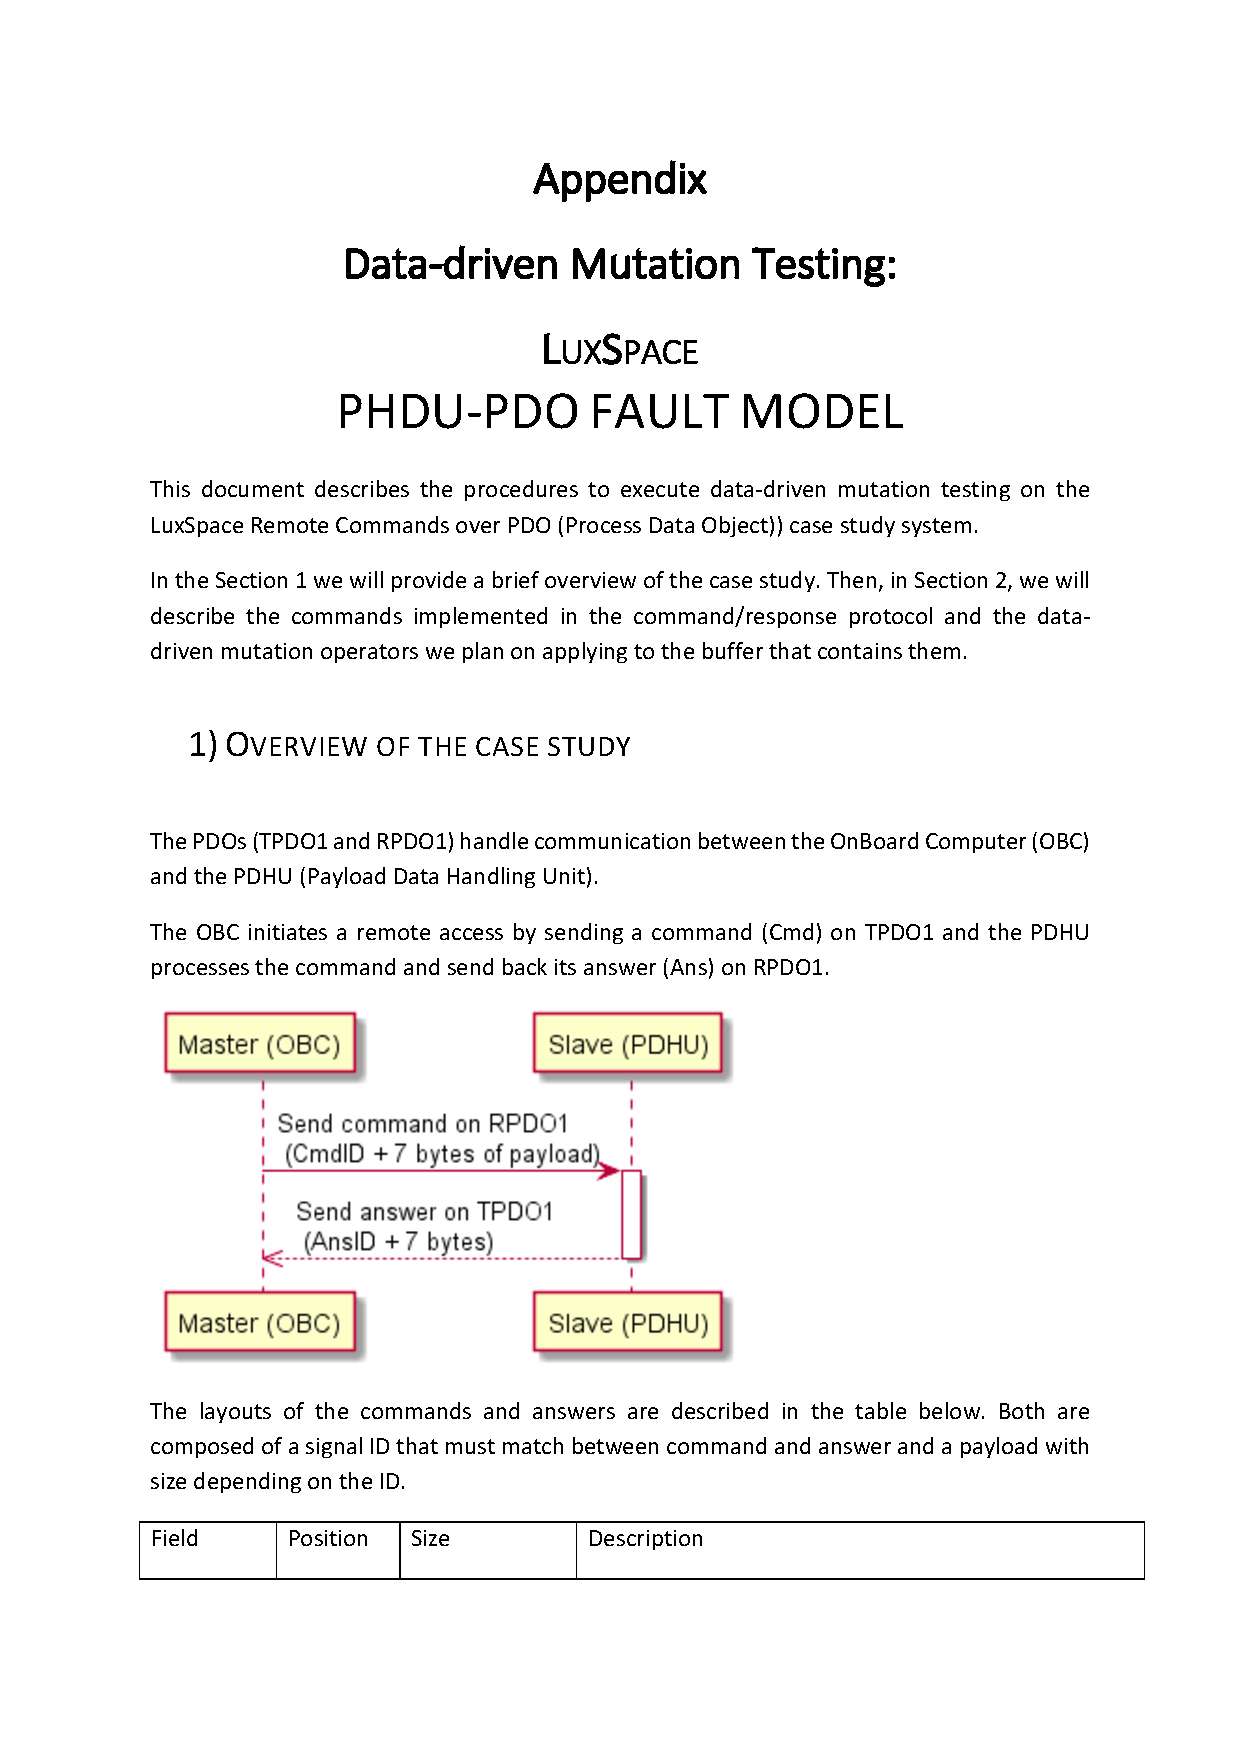
\includepdf[pages=-,scale=0.9,offset=0mm -75]{faultModels/ESAIL_PHDU_PDO_Fault_Model.pdf}

\section{GomSpace LibGCSP Fault Model Description}

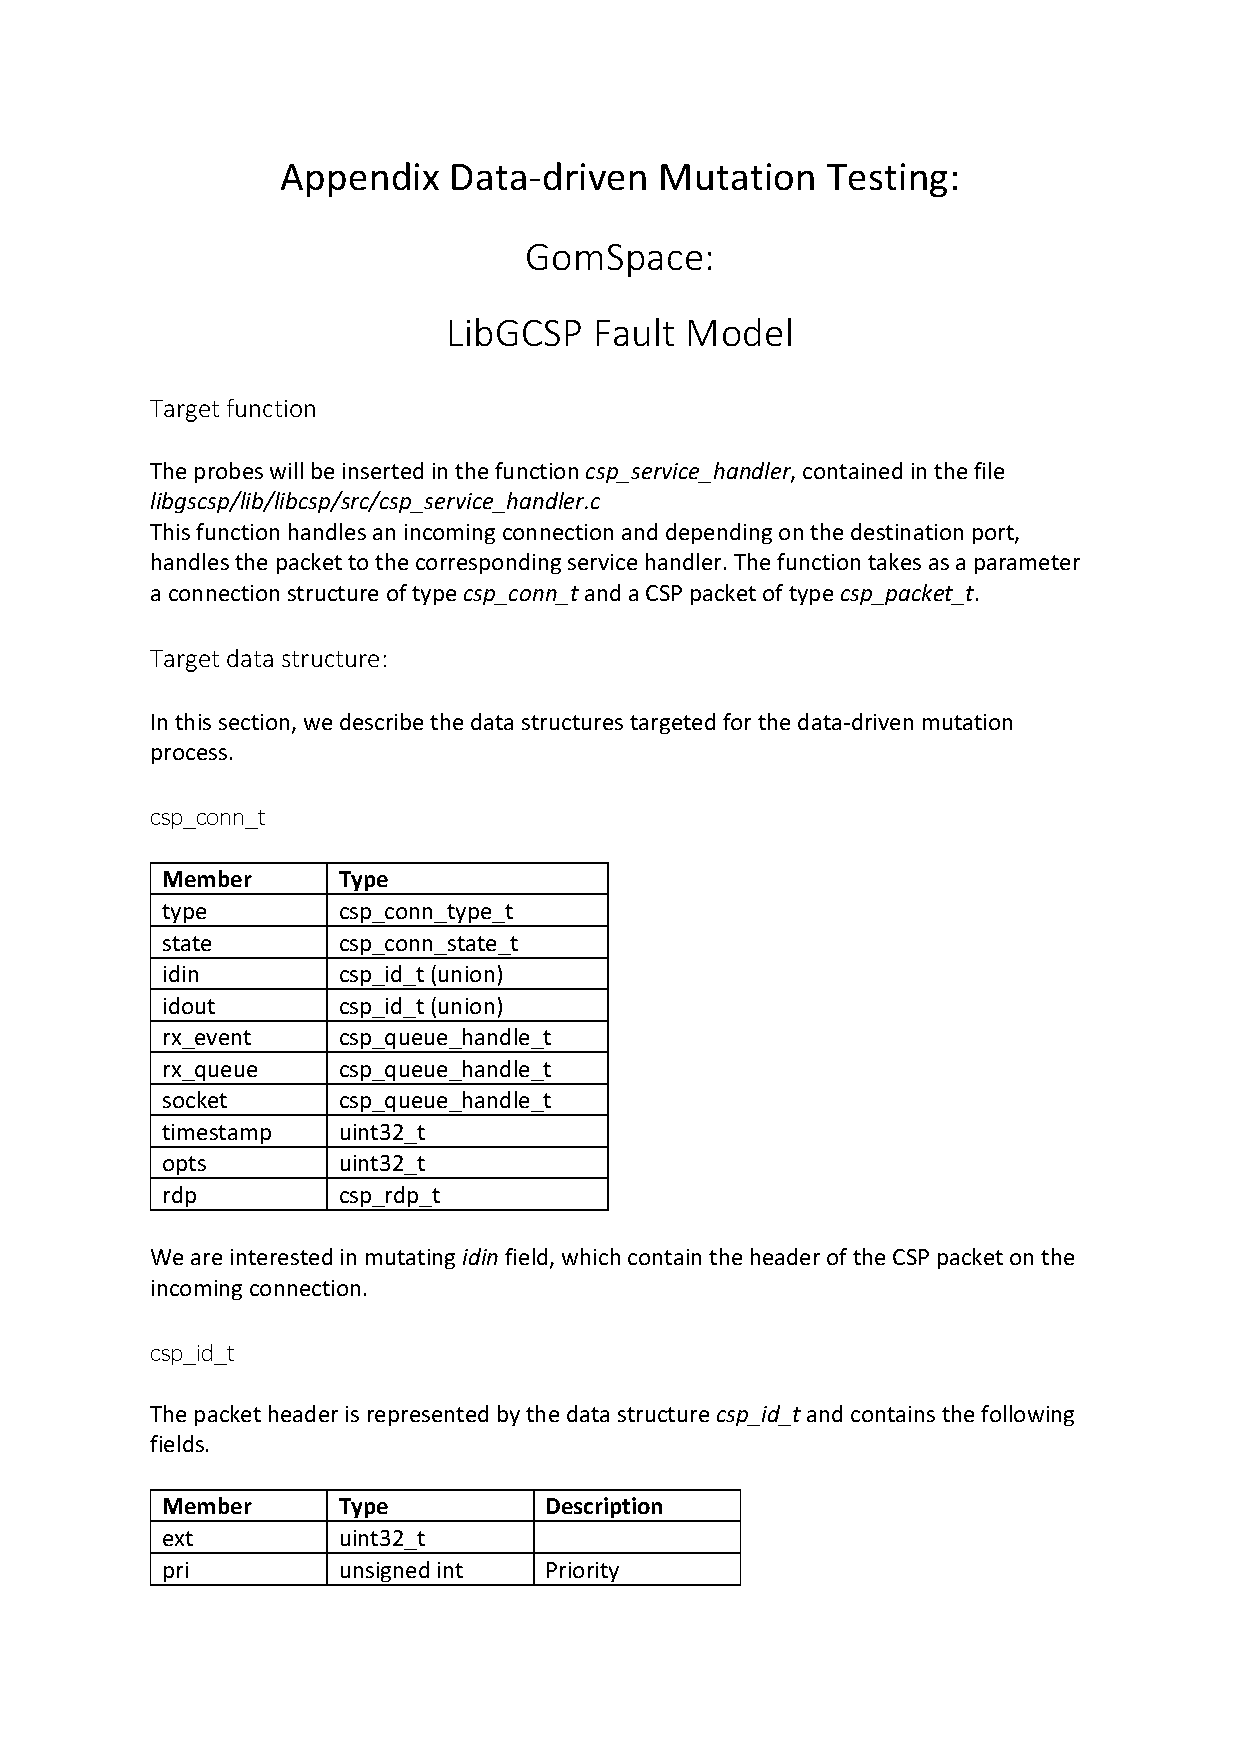
\includepdf[pages=-,scale=0.9,offset=0mm -75]{faultModels/LibGSCSPFaultModel.pdf}

\section{GomSpace LibParam Fault Model Description}

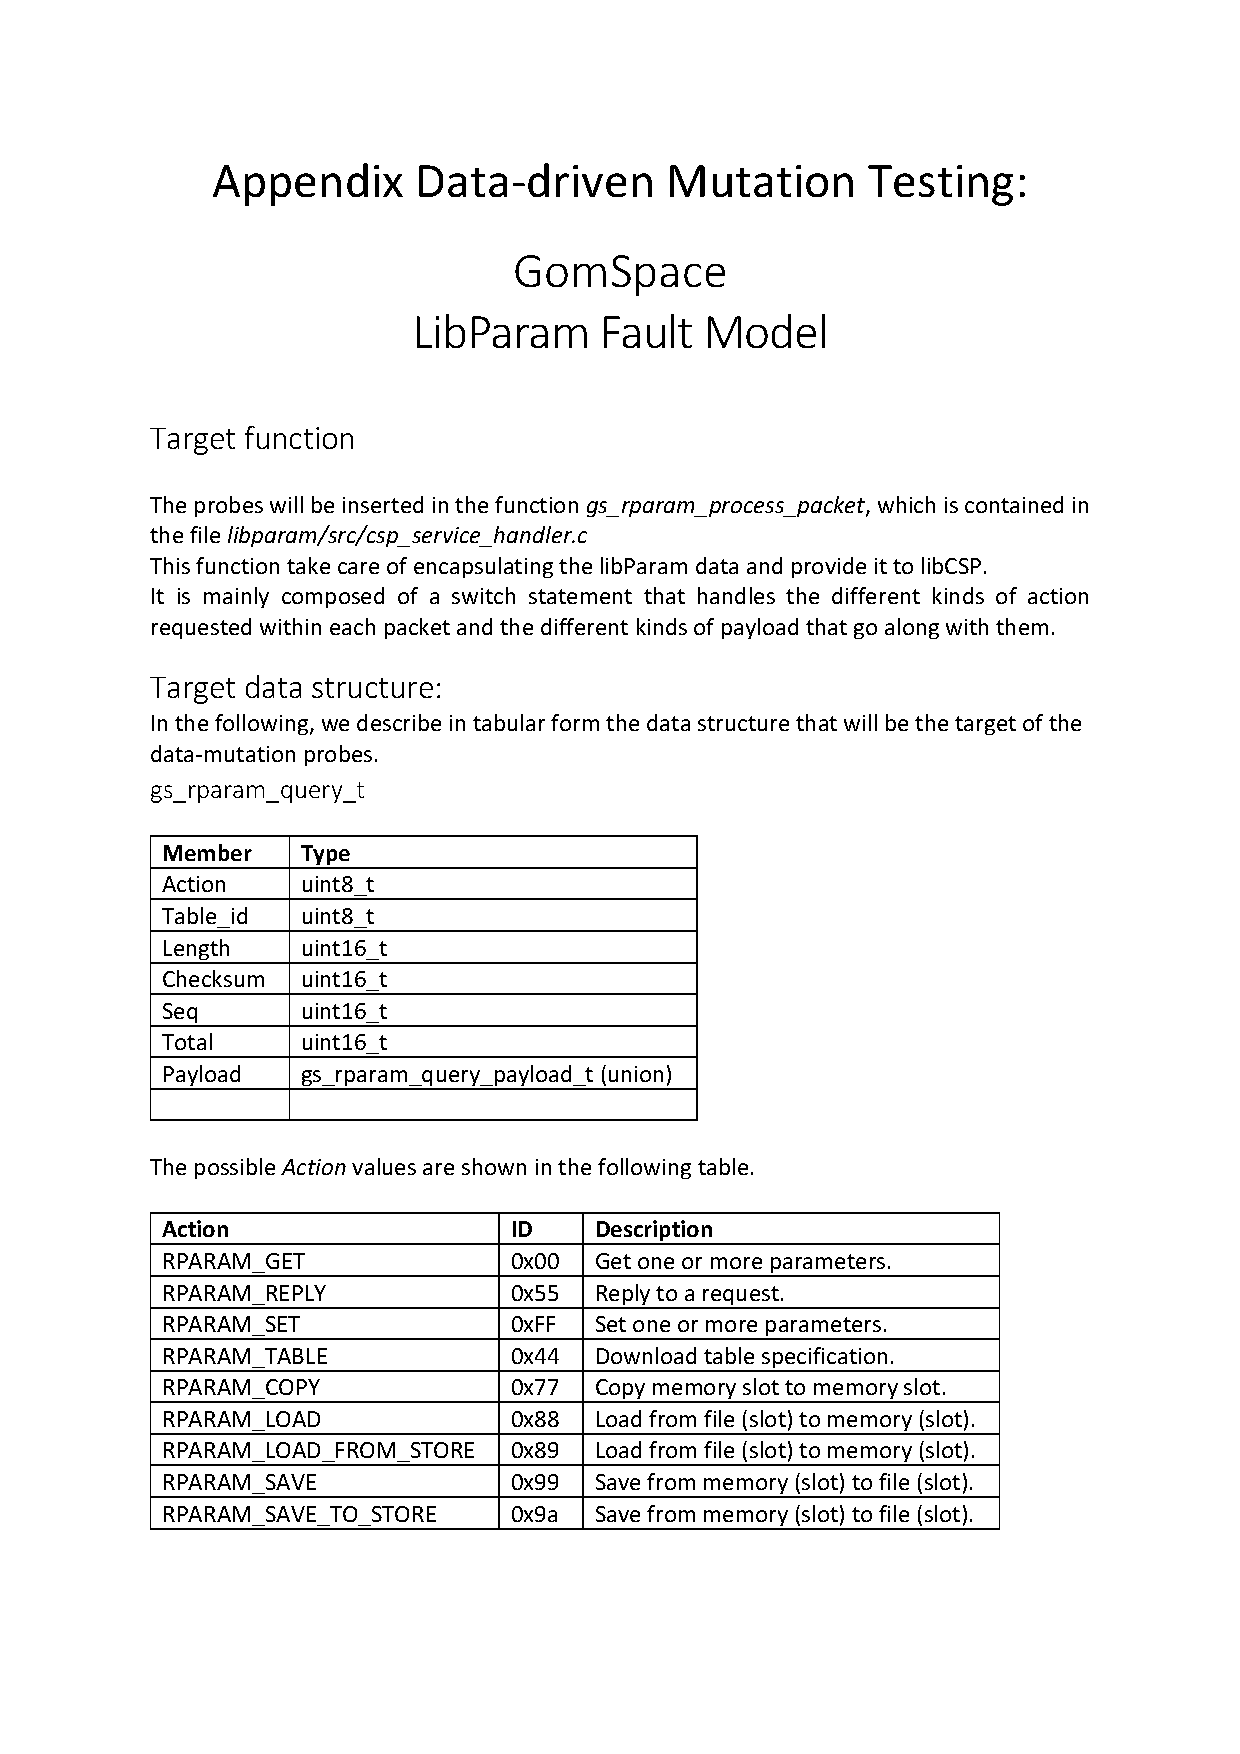
\includepdf[pages=-,scale=0.9,offset=0mm -75]{faultModels/LibParamFaultModel.pdf}

\section{Tabular Fault Models}

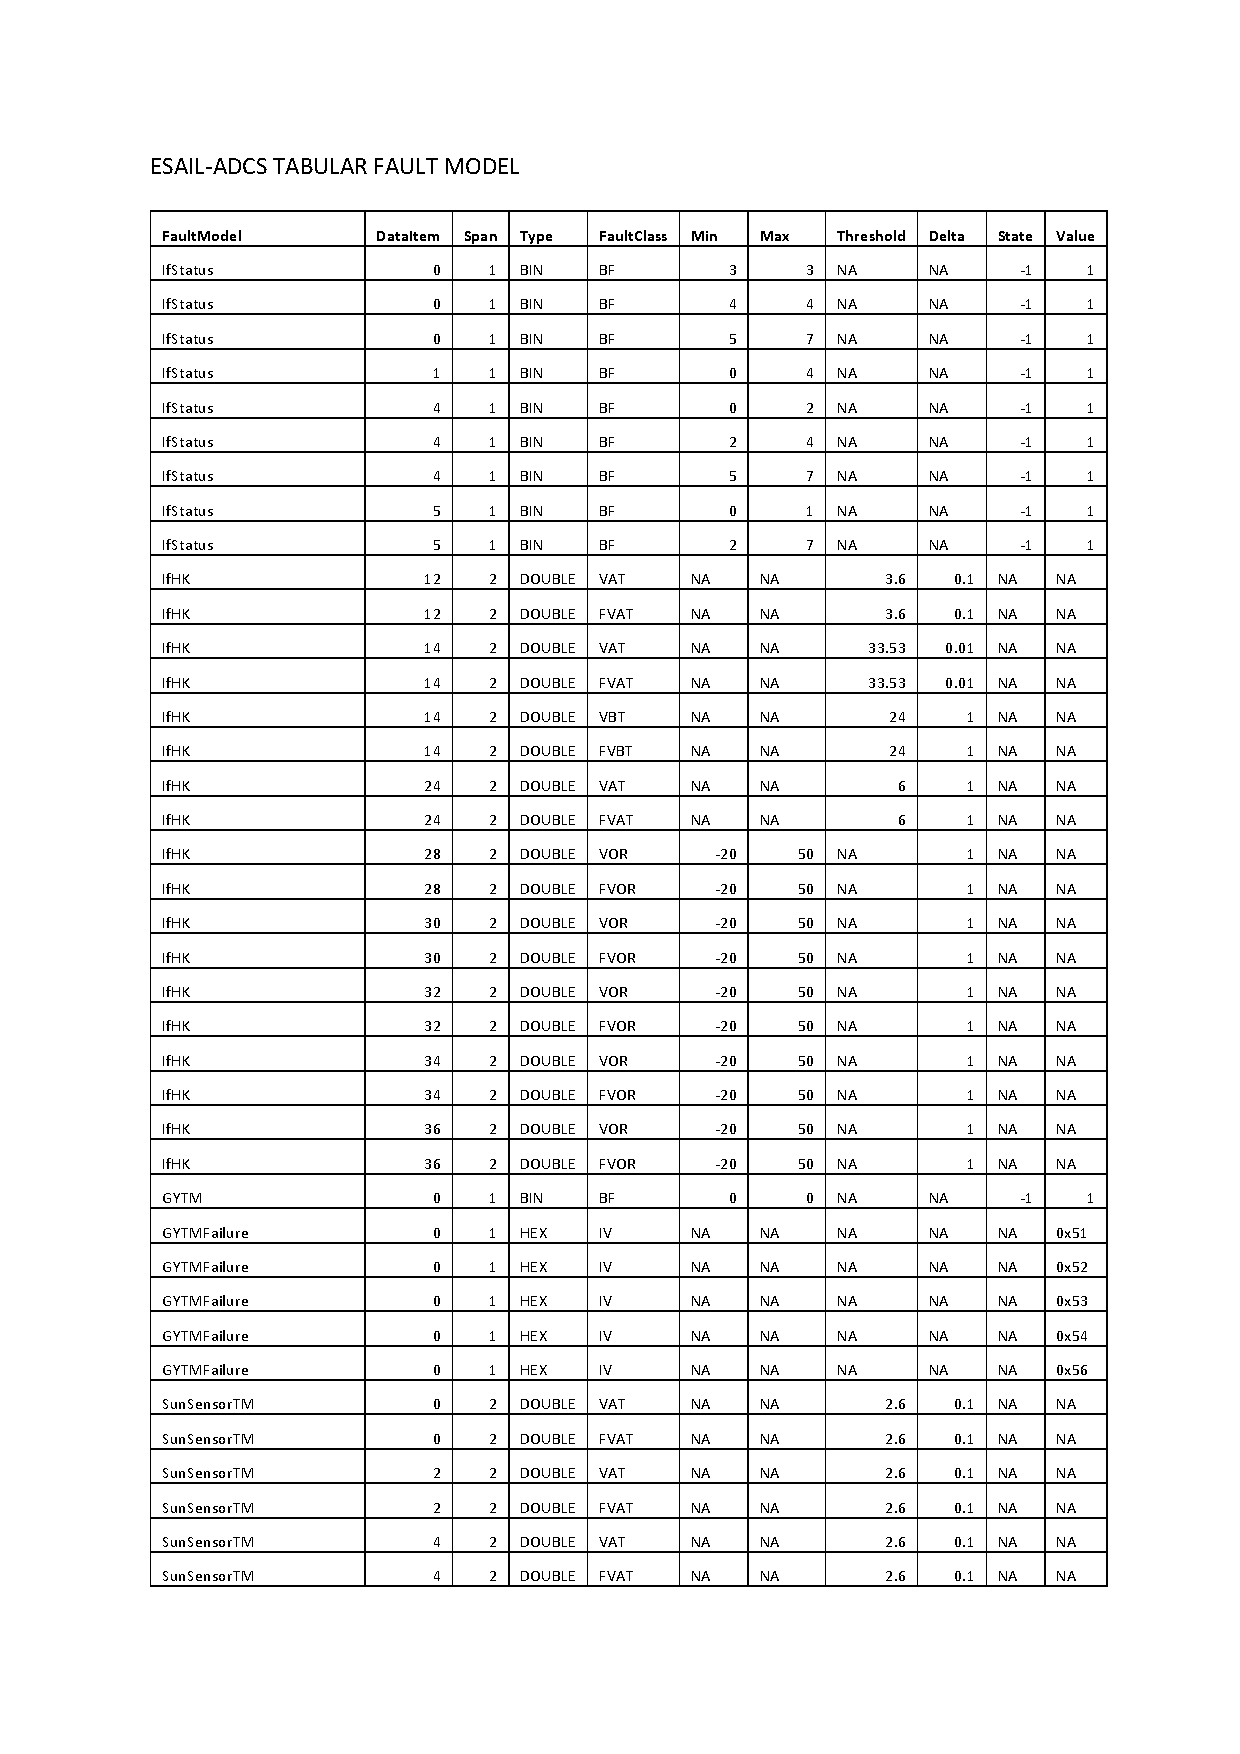
\includepdf[pages=-,scale=0.9,offset=0mm -75]{faultModels/FaultModels.pdf}

\textbf{End of Appendix}

   
\clearpage
% !TEX root = MAIN.tex
\chapter{ESA Revisions}

%% !TEX root = MAIN.tex

\section{Responses to ESA comments provided on 12.04.2021}
\label{sec:ESA:comments:1}

Comments IDs appear also in the main document next to the text modified to address the comment. To save space in the main text, the prefix \emph{ITSR-SSS-PABG-} has been abbreviated as \emph{P-}.

\setlength\LTleft{0pt}
\setlength\LTright{0pt}
\tiny 
%@{\extracolsep{\fill}}
\begin{longtable}{|p{1.5cm}|p{12cm}|@{}}
%\caption{\normalsize .}
%\label{table:comments:responses} 
\textbf{Comment ID}&\textbf{Response}\\
\\
\hline
P-1&
\begin{minipage}{12cm}
We will need to discuss the detail of the merge of the two specifications during the review meeting.
\end{minipage}\\
\\
\hline

P-2&
\begin{minipage}{12cm}
Done.
\end{minipage}\\
\\
\hline

P-3&
\begin{minipage}{12cm}
Done.
\end{minipage}\\
\\
\hline

P-4&
\begin{minipage}{12cm}
Done.
\end{minipage}\\
\\
\hline

P-5&
\begin{minipage}{12cm}
Done.
\end{minipage}\\
\\
\hline

P-6&
\begin{minipage}{12cm}
Done.
\end{minipage}\\
\\
\hline

P-7&
\begin{minipage}{12cm}
Done.
\end{minipage}\\
\\
\hline

P-8&
\begin{minipage}{12cm}
Done.
\end{minipage}\\
\\
\hline

P-9&
\begin{minipage}{12cm}
It is worth discussing if it makes sense to perform mutation analysis without code coverage.
\end{minipage}\\
\\
\hline


P-10&
\begin{minipage}{12cm}
We always generate all the mutants because it's fast. End-users have the option to execute a subset of them.
\end{minipage}\\
\\
\hline

P-11&
\begin{minipage}{12cm}
We changed a sentence, but this requirement is long because we had to provide an explanation missing from D2.
\end{minipage}\\
\\
\hline

P-12&
\begin{minipage}{12cm}
\end{minipage}\\
\\
\hline

P-13&
\begin{minipage}{12cm}
\end{minipage}\\
See P-8\\
\hline

P-14&
\begin{minipage}{12cm}
\end{minipage}\\
Action item. To be done for the end of WP3.\\
\hline


P-15&
\begin{minipage}{12cm}
TOD
\end{minipage}\\
\hline

P-16&
\begin{minipage}{12cm}
Done.
\end{minipage}\\
\hline

P-17&
\begin{minipage}{12cm}
We will provide a table for end of WP3.
\end{minipage}\\
\hline
                                                
\end{longtable}
\normalsize

\clearpage

% !TEX root = MutationTestingSurvey.tex

\section{Responses to ESA comments provided on 03.04.2020}
\label{sec:ESA:comments:2}


\setlength\LTleft{0pt}
\setlength\LTright{0pt}
\tiny 
\begin{longtable}{|p{1.5cm}|p{12cm}|@{}}
\label{table:comments:responses} 
\textbf{Comment ID}&\textbf{Comment and Response (below)}\\
\\
\midrule
C6 \& C7
&
Have you seen numbers for this mutation score and threshold in the literature? Is this something to be checked during the use case evaluation?
\\
\cmidrule{2-2}
&
We have addressed the comments above.
\TODO{OScar: please check if the survey of Papadakis say something aboth teh threshold (C7)}
\\
\hline
C8
&
Elaborate a bit more on C8 (pros and cons of doing mutation at source code / IR/ Assembly/ Executable);
\\
\cmidrule{2-2}
&
\TODO{Oscar: you may refer to taht paper of Darko Marinov and Co. to say IR is not good}
\\
\hline
C31
&
What is this sufficient set of operators?
\\
\cmidrule{2-2}
&
\TODO{Oscar}
\\
\hline
C32
&
Can you please add the solution for this example? i.e. do we need two different test cases of isPalindrome to detect both mutants?
\\
\cmidrule{2-2}
&
\TODO{Oscar}
\\
\hline
C33
&
Even if the objectives are complementary, both of them should be pursued for a data mutation testing approach?
\\
\cmidrule{2-2}
&
We have addressed the comment above.
\\
\hline
C34
&
The sentence sounds weird... To automate?? Is this activity something that can be automated?
\\
\cmidrule{2-2}
&
We have addressed the comment above by clarifying our text.
\\
\hline
C35
&
Is it possible to add an example of equivalent and redundant mutants?
\\
\cmidrule{2-2}
&
We have added the requested examples.
\\
\hline
C36
&
\begin{minipage}{12cm}
Related to automation, in my opinion, what it is key is that the test assessment process (for both data and code mutation) is as much automated as possible.\\

Automated generation of test cases is a very nice to have. In an industrial environment, let's say that we could afford spending some time to manually augment the test suite.\\

You may consider this to prioritize tasks within this activity.
\end{minipage}
\\
\cmidrule{2-2}
&
We agree on the comment. No need to change the text in this deliverable.
\\
\hline
C37
&
Are we missing a chapter to address the Generation of Test Oracles?\\
\cmidrule{2-2}
&
We have added a section concerning generation of test oracles for code-driven mutation testing (Section~\ref{sec:oraclesGeneration:codeDriven}) and data-driven mutation testing 
(Section~\ref{sec:oracles:dataMutation}).
\\
\hline
C38
&
\begin{minipage}{12cm}
a. From these Case Studies, is there any that you would like to try out within FAQAS?\\

b. One thing that we may need for FAQAS framework is to have kind of a test suite allowing to test the tool, and also to test the tool when new versions will be produced. Would any of these case studies fulfill that?
\end{minipage}
\\
\cmidrule{2-2}
&
We have discussed this topics by voice.
\\
\hline
C39
&
Do you have any information on the kind of test suite? (e.g. is it unit testing, system testing, ...)
\\
\cmidrule{2-2}
&
\TODO{}
\\
\hline
C40
&
Are these case studies focused on Code-Mutation, Data-Mutation, or both?\\
\cmidrule{2-2}
&
\TODO{}
\\
\hline
C41
&
Is there any meaningful conclusion (positive or negative) from those industrial case studies?\\
\cmidrule{2-2}
&
\TODO{}
\\
\hline
C42
&
\begin{minipage}{12cm}
Can we make a conclusion paragraph on this?\\

e.g. No tool based on mutation testing is known to be used within an industrial software development environment\\
e.g. Mutation testing is seen applied mainly within research environments\\
etc, etc
\end{minipage}
\\
\cmidrule{2-2}
&
\TODO{}
\\
\hline
C43
&
Is there any of these trends that could be meaningful to explore?
\\
\cmidrule{2-2}
&
\TODO{}
\\
\hline
C44
&
\begin{minipage}{12cm}
	\begin{itemize}
		\item Is there any particular trend for Code-Based mutation testing? (e.g. research is on-going or vanishing, the way to apply it, the type of operators used, the tools supporting it, ...)
		\item Any particular trend for Data-Based mutation testing?
	\end{itemize}
\end{minipage}
\\
\cmidrule{2-2}
&
\TODO{}
\\
\hline
C45&
\begin{minipage}{12cm}
D1 is fulfilling well requirement R1-1 as in the SoW. There is only one exception, on the red sentence below:\\

[R1-1.c] The applications of mutation testing (e.g. code and data mutation, test-suite evaluation, test cases generation, test-data generation, \textcolor{red}{code quality improvement}, ...)\\

The evaluation of code quality improvement is to be looked at. Indeed, this would be a secondary objective of applying mutation testing on space systems, but we would like to understand if mutation testing could help improve the code quality or not.\\
\end{minipage}
\\
\cmidrule{2-2}
&
\begin{minipage}{12cm}
We added a paragraph on Chapter~\ref{chapter:trends} explaining that there are no works in literature about quality code improvement based on code-driven mutation testing.
\end{minipage}
\\

\bottomrule                                                             
\end{longtable}
\normalsize

\clearpage


\clearpage

\printindex

\bibliographystyle{IEEEtran}
\bibliography{bibliography}


\end{document}  